% ------------------------------------------------------------
% LaTeX Template für die DHBW zum Schnellstart!
% Original: https://github.wdf.sap.corp/vtgermany/LaTeX-Template-DHBW
% ------------------------------------------------------------
% ---- Präambel mit Angaben zum Dokument
\documentclass[
	fontsize=12pt,           % Leitlinien sprechen von Schriftgröße 12.
	paper=A4,
	twoside=false,
	listof=totoc,            % Tabellen- und Abbildungsverzeichnis ins Inhaltsverzeichnis
	bibliography=totoc,      % Literaturverzeichnis ins Inhaltsverzeichnis aufnehmen
	titlepage,               % Titlepage-Umgebung anstatt \maketitle
	headsepline,             % horizontale Linie unter Kolumnentitel
	abstract,              % Überschrift einschalten, Abstract muss in {abstract}-Umgebung stehen
]{scrreprt}                  % Verwendung von KOMA-Report
\usepackage[utf8]{inputenc}  % UTF8 Encoding einschalten
\usepackage[ngerman]{babel}  % Neue deutsche Rechtschreibung
\usepackage[T1]{fontenc}     % Ausgabe von westeuropäischen Zeichen (auch Umlaute)
\usepackage{microtype}       % Trennung von Wörtern wird besser umgesetzt
\usepackage{lmodern}         % Nicht-gerasterte Schriftarten (bei MikTeX erforderlich)
\usepackage{graphicx}        % Einbinden von Grafiken erlauben
\usepackage{wrapfig}         % Grafiken fließend im Text
\usepackage{setspace}        % Zeilenabstand \singlespacing, \onehalfspaceing, \doublespacing
\usepackage[
	%showframe,                % Ränder anzeigen lassen
	left=2.7cm, right=2.5cm,
	top=2.5cm,  bottom=2.5cm,
	includeheadfoot
]{geometry}                      % Seitenlayout einstellen
\usepackage{scrlayer-scrpage}    % Gestaltung von Fuß- und Kopfzeilen
\usepackage{acronym}             % Abkürzungen, Abkürzungsverzeichnis
\usepackage{titletoc}            % Anpassungen am Inhaltsverzeichnis
\contentsmargin{0.75cm}          % Abstand im Inhaltsverzeichnis zw. Punkt und Seitenzahl
\usepackage[                     % Klickbare Links (enth. auch "nameref", "url" Package)
  hidelinks,                     % Blende die "URL Boxen" aus.
  breaklinks=true                % Breche zu lange URLs am Zeilenende um
]{hyperref}
\usepackage[hypcap=true]{caption}% Anker Anpassung für Referenzen
\urlstyle{same}                  % Aktuelle Schrift auch für URLs
% Anpassung von autoref für Gleichungen (ergänzt runde Klammern) und Algorithm.
% Anstatt "Listing" kann auch z.B. "Code-Ausschnitt" verwendet werden. Dies sollte
% jedoch synchron gehalten werden mit \lstlistingname (siehe weiter unten).
\addto\extrasngerman{%
	\def\equationautorefname~#1\null{Gleichung~(#1)\null}
	\def\lstnumberautorefname{Zeile}
	\def\lstlistingautorefname{Code-Ausschnitt}
	\def\algorithmautorefname{Algorithmus}
	% Damit einheitlich "Abschnitt 1.2[.3]" verwendet wird und nicht "Unterabschnitt 1.2.3"
	% \def\subsectionautorefname{Abschnitt}
}

% ---- Abstand verkleinern von der Überschrift 
\renewcommand*{\chapterheadstartvskip}{\vspace*{.5\baselineskip}}

% Hierdurch werden Schusterjungen und Hurenkinder vermieden, d.h. einzelne Wörter
% auf der nächsten Seite oder in einer einzigen Zeile.
% LaTeX kann diese dennoch erzeugen, falls das Layout ansonsten nicht umsetzbar ist.
% Diese Werte sind aber gute Startwerte.
\widowpenalty10000
\clubpenalty10000

% ---- Für das Quellenverzeichnis
\usepackage[
	backend = biber,                % Verweis auf biber
	language = auto,
	style = numeric,                % Nummerierung der Quellen mit Zahlen
	sorting = none,                 % none = Sortierung nach der Erscheinung im Dokument
	sortcites = true,               % Sortiert die Quellen innerhalb eines cite-Befehls
	block = space,                  % Extra Leerzeichen zwischen Blocks
	hyperref = true,                % Links sind klickbar auch in der Quelle
	%backref = true,                % Referenz, auf den Text an die zitierte Stelle
	bibencoding = auto,
	giveninits = true,              % Vornamen werden abgekürzt
	doi=false,                      % DOI nicht anzeigen
	isbn=false,                     % ISBN nicht anzeigen
    alldates=short                  % Datum immer als DD.MM.YYYY anzeigen
]{biblatex}
\addbibresource{Inhalt/literatur.bib}
\setcounter{biburlnumpenalty}{3000}     % Umbruchgrenze für Zahlen
\setcounter{biburlucpenalty}{6000}      % Umbruchgrenze für Großbuchstaben
\setcounter{biburllcpenalty}{9000}      % Umbruchgrenze für Kleinbuchstaben
\DeclareNameAlias{default}{family-given}  % Nachname vor dem Vornamen
\AtBeginBibliography{\renewcommand{\multinamedelim}{\addslash\space
}\renewcommand{\finalnamedelim}{\multinamedelim}}  % Schrägstrich zwischen den Autorennamen
\DefineBibliographyStrings{german}{
  urlseen = {Einsichtnahme:},                      % Ändern des Titels von "besucht am"
}
\usepackage[babel,german=quotes]{csquotes}         % Deutsche Anführungszeichen + Zitate


% ---- Für Mathevorlage
\usepackage{amsmath}    % Erweiterung vom Mathe-Satz
\usepackage{amssymb}    % Lädt amsfonts und weitere Symbole
\usepackage{MnSymbol}   % Für Symbole, die in amssymb nicht enthalten sind.


% ---- Für Quellcodevorlage
\usepackage{scrhack}                    % Hack zur Verw. von listings in KOMA-Script
\usepackage{listings}                   % Darstellung von Quellcode
\usepackage{xcolor}                     % Einfache Verwendung von Farben
% -- Eigene Farben für den Quellcode
\definecolor{JavaLila}{rgb}{0.4,0.1,0.4}
\definecolor{JavaGruen}{rgb}{0.3,0.5,0.4}
\definecolor{JavaBlau}{rgb}{0.0,0.0,1.0}
\definecolor{greenString}{HTML}{13752f}
\definecolor{ABAPKeywordsBlue}{HTML}{6000ff}
\definecolor{ABAPCommentGrey}{HTML}{808080}
\definecolor{ABAPStringGreen}{HTML}{4da619}
\definecolor{PyKeywordsBlue}{HTML}{0000AC}
\definecolor{PyCommentGrey}{HTML}{808080}
\definecolor{PyStringGreen}{HTML}{008080}
% -- Farben für ABAP CDS
\definecolor{CDSString}{HTML}{FF8C00}
\definecolor{CDSKeywords}{HTML}{6000ff}
\definecolor{CDSAnnotation}{HTML}{00BFFF}
\definecolor{CDSComment}{HTML}{808080}
\definecolor{CDSFunc}{HTML}{FF0000}

% -- Default Listing-Styles

\lstset{
	% Das Paket "listings" kann kein UTF-8. Deswegen werden hier 
	% die häufigsten Zeichen definiert (ä,ö,ü,...)
	literate=%
		{á}{{\'a}}1 {é}{{\'e}}1 {í}{{\'i}}1 {ó}{{\'o}}1 {ú}{{\'u}}1
		{Á}{{\'A}}1 {É}{{\'E}}1 {Í}{{\'I}}1 {Ó}{{\'O}}1 {Ú}{{\'U}}1
		{à}{{\`a}}1 {è}{{\`e}}1 {ì}{{\`i}}1 {ò}{{\`o}}1 {ù}{{\`u}}1
		{À}{{\`A}}1 {È}{{\'E}}1 {Ì}{{\`I}}1 {Ò}{{\`O}}1 {Ù}{{\`U}}1
		{ä}{{\"a}}1 {ë}{{\"e}}1 {ï}{{\"i}}1 {ö}{{\"o}}1 {ü}{{\"u}}1
		{Ä}{{\"A}}1 {Ë}{{\"E}}1 {Ï}{{\"I}}1 {Ö}{{\"O}}1 {Ü}{{\"U}}1
		{â}{{\^a}}1 {ê}{{\^e}}1 {î}{{\^i}}1 {ô}{{\^o}}1 {û}{{\^u}}1
		{Â}{{\^A}}1 {Ê}{{\^E}}1 {Î}{{\^I}}1 {Ô}{{\^O}}1 {Û}{{\^U}}1
		{œ}{{\oe}}1 {Œ}{{\OE}}1 {æ}{{\ae}}1 {Æ}{{\AE}}1 {ß}{{\ss}}1
		{ű}{{\H{u}}}1 {Ű}{{\H{U}}}1 {ő}{{\H{o}}}1 {Ő}{{\H{O}}}1
		{ç}{{\c c}}1 {Ç}{{\c C}}1 {ø}{{\o}}1 {å}{{\r a}}1 {Å}{{\r A}}1
		{€}{{\euro}}1 {£}{{\pounds}}1 {«}{{\guillemotleft}}1
		{»}{{\guillemotright}}1 {ñ}{{\~n}}1 {Ñ}{{\~N}}1 {¿}{{?`}}1,
	breaklines=true,        % Breche lange Zeilen um 
	breakatwhitespace=true, % Wenn möglich, bei Leerzeichen umbrechen
	% Symbol für Zeilenumbruch einfügen
	prebreak=\raisebox{0ex}[0ex][0ex]{\ensuremath{\rhookswarrow}},
	postbreak=\raisebox{0ex}[0ex][0ex]{\ensuremath{\rcurvearrowse\space}},
	tabsize=4,                                 % Setze die Breite eines Tabs
	basicstyle=\ttfamily\small,                % Grundsätzlicher Schriftstyle
	columns=fixed,                             % Besseres Schriftbild
	numbers=left,                              % Nummerierung der Zeilen
	%frame=single,                             % Umrandung des Codes
	showstringspaces=false,                    % Keine Leerzeichen hervorheben
	keywordstyle=\color{blue},
	ndkeywordstyle=\bfseries\color{darkgray},
	identifierstyle=\color{black},
	commentstyle=\itshape\color{JavaGruen},   % Kommentare in eigener Farbe
	stringstyle=\color{JavaBlau},             % Strings in eigener Farbe,
	captionpos=b,                             % Bild*unter*schrift
	xleftmargin=5.0ex
}

% ---- Eigener JAVA-Style für den Quellcode
\renewcommand{\ttdefault}{pcr}               % Schriftart, welche auch fett beinhaltet
\lstdefinestyle{EigenerJavaStyle}{
	language=Java,                             % Syntax Highlighting für Java
	%frame=single,                             % Umrandung des Codes
	keywordstyle=\bfseries\color{JavaLila},    % Keywords in eigener Farbe und fett
	commentstyle=\itshape\color{JavaGruen},    % Kommentare in eigener Farbe und italic
	stringstyle=\color{JavaBlau}               % Strings in eigener Farbe
}

% ---- Eigener ABAP-Style für den Quellcode
\renewcommand{\ttdefault}{pcr}
\lstdefinestyle{EigenerABAPStyle}{
	language=[R/3 6.10]ABAP,
	morestring=[b]\|,                          % Für Pipe-Strings
	morestring=[b]\`,                          % für Backtick-Strings
	keywordstyle=\bfseries\color{ABAPKeywordsBlue},
	commentstyle=\itshape\color{ABAPCommentGrey},
	stringstyle=\color{ABAPStringGreen},
	tabsize=2,
	morekeywords={
		types,
		@data,
		as,
		lower,
		start,
		selection,
		order,
		by,
		inner,
		join,
		key,
		end,
		cast
	}
}

% ---- Eigener Python-Style für den Quellcode
\renewcommand{\ttdefault}{pcr}
\lstdefinestyle{EigenerPythonStyle}{
	language=Python,
	columns=flexible,
	keywordstyle=\bfseries\color{PyKeywordsBlue},
	commentstyle=\itshape\color{PyCommentGrey},
	stringstyle=\color{PyStringGreen}
}

% ---- Eigener Cpp-Style für den Quellcode
\renewcommand{\ttdefault}{pcr}
\lstdefinestyle{EigenerCppStyle}{
	language=C++,
	columns=flexible,
	keywordstyle=\bfseries\color{JavaLila},    % Keywords in eigener Farbe und fett
	commentstyle=\itshape\color{JavaGruen},    % Kommentare in eigener Farbe und italic
	stringstyle=\color{greenString}               % Strings in eigener Farbe
}

% ---- Eigener Go-Style für den Quellcode
\renewcommand{\ttdefault}{pcr}
\lstdefinestyle{EigenerGoStyle}{
	language=Go,
	columns=flexible,
	keywordstyle=\bfseries\color{JavaLila},    % Keywords in eigener Farbe und fett
	commentstyle=\itshape\color{JavaGruen},    % Kommentare in eigener Farbe und italic
	stringstyle=\color{greenString}               % Strings in eigener Farbe
}

% ---- Eigener Json-Style für den Quellcode
\renewcommand{\ttdefault}{pcr}
\lstdefinestyle{EigenerJsonStyle}{
	language=Go,
	columns=flexible,
	keywordstyle=\bfseries\color{JavaLila},    % Keywords in eigener Farbe und fett
	commentstyle=\itshape\color{JavaGruen},    % Kommentare in eigener Farbe und italic
	stringstyle=\color{greenString}               % Strings in eigener Farbe
}

%----- ABAP-CDS-View language
\lstdefinelanguage{ABAPCDS}{
	sensitive=false,
	%Keywords
	morekeywords={define,
		view,
		as,
		select,
		from,
		inner,
		join,
		on,
		key,
		case,
		when,
		then,
		else,
		end,
		true,
		false,
		cast,
		where,
		and,
		distinct,
		group,
		by,
		having,
		min,
		sum,
		max,
		count,
		avg
	},
	%Methoden
	morekeywords=[2]{
		div,
		currency\_conversion,
		dats\_days\_between,
		concat\_with\_space,
		dats\_add_days,
		dats\_is\_valid,
		dats\_add\_months,
		unit\_conversion,
		division,
		mod,
		abs,
		floor,
		ceil,
		round,
		concat,
		replace,
		substring,
		left,
		right,
		length
	},
	morecomment=[s][\color{CDSAnnotation}]{@}{:},
	morecomment=[l][\itshape\color{CDSComment}]{//},
	morecomment=[s][\itshape\color{CDSComment}]{/*}{*/},
	morestring=[b][\color{CDSString}]',
	keywordstyle=\bfseries\color{CDSKeywords},
	keywordstyle=[2]\color{CDSFunc}
}

  % Weitere Details sind ausgelagert

\usepackage{algorithm}                  % Für Algorithmen-Umgebung (ähnlich wie lstlistings Umgebung)
\usepackage{algpseudocode}              % Für Pseudocode. Füge "[noend]" hinzu, wenn du kein "endif",
                                        % etc. haben willst.

\makeatletter                           % Sorgt dafür, dass man @ in Namen verwenden kann.
                                        % Ansonsten gibt es in der nächsten Zeile einen Compilefehler.
\renewcommand{\ALG@name}{Algorithmus}   % Umbenennen von "Algorithm" im Header der Listings.
\makeatother                            % Zeichen wieder zurücksetzen
\renewcommand{\lstlistingname}{Code-Ausschnitt} % Erlaubt das Umbenennen von "Listing" in anderen Titel.

% ---- Tabellen
\usepackage{booktabs}  % Für schönere Tabellen. Enthält neue Befehle wie \midrule
\usepackage{multirow}  % Mehrzeilige Tabellen
\usepackage{siunitx}   % Für SI Einheiten und das Ausrichten Nachkommastellen
\sisetup{locale=DE, range-phrase={~bis~}, output-decimal-marker={,}} % Damit ein Komma und kein Punkt verwendet wird.
\usepackage{xfrac} % Für siunitx Option "fraction-function=\sfrac"

% ---- Für Definitionsboxen in der Einleitung
\usepackage{amsthm}                     % Liefert die Grundlagen für Theoreme
\usepackage[framemethod=tikz]{mdframed} % Boxen für die Umrandung
% ---- Definition für Highlight Boxen

% ---- Grundsätzliche Definition zum Style
\newtheoremstyle{defi}
  {\topsep}         % Abstand oben
  {\topsep}         % Abstand unten
  {\normalfont}     % Schrift des Bodys
  {0pt}             % Einschub der ersten Zeile
  {\bfseries}       % Darstellung von der Schrift in der Überschrift
  {:}               % Trennzeichen zwischen Überschrift und Body
  {.5em}            % Abstand nach dem Trennzeichen zum Body Text
  {\thmname{#3}}    % Name in eckigen Klammern
\theoremstyle{defi}

% ------ Definition zum Strich vor eines Texts
\newmdtheoremenv[
  hidealllines = true,       % Rahmen komplett ausblenden
  leftline = true,           % Linie links einschalten
  innertopmargin = 0pt,      % Abstand oben
  innerbottommargin = 4pt,   % Abstand unten
  innerrightmargin = 0pt,    % Abstand rechts
  linewidth = 3pt,           % Linienbreite
  linecolor = gray!40,       % Linienfarbe
]{defStrich}{Definition}     % Name der des formats "defStrich"

% ------ Definition zum Eck-Kasten um einen Text
\newmdtheoremenv[
  hidealllines = true,
  innertopmargin = 6pt,
  linecolor = gray!40,
  singleextra={              % Eck-Markierungen für die Definition
    \draw[line width=3pt,gray!50,line cap=rect] (O|-P) -- +(1cm,0pt);
    \draw[line width=3pt,gray!50,line cap=rect] (O|-P) -- +(0pt,-1cm);
    \draw[line width=3pt,gray!50,line cap=rect] (O-|P) -- +(-1cm,0pt);
    \draw[line width=3pt,gray!50,line cap=rect] (O-|P) -- +(0pt,1cm);
  }
]{defEckKasten}{Definition}  % Name der des formats "defEckKasten"  % Weitere Details sind ausgelagert

% ---- Für Todo Notes
\usepackage{todonotes}
\setlength {\marginparwidth }{2cm}      % Abstand für Todo Notizen

% ---- Für PDFs-Anhängen
\usepackage{pdfpages}

% ---- Elektronische Version oder Gedruckte Version?
% ---- Unterschied: Die elektronische Version enthält keinen Platzhalter für die Unterschrift
\usepackage{ifthen}
\newboolean{e-Abgabe}
\setboolean{e-Abgabe}{false}    % false=gedruckte Fassung

% ---- Persönlichen Daten:
\newcommand{\titel}{Erkennung fahrradfreundlicher, städtischer Wege mithilfe von Computer Vision über Luftaufnahmen}
\newcommand{\titelheader}{Studienarbeit}
\newcommand{\arbeit}{Studienarbeit}
\newcommand{\studiengang}{Informatik}
\newcommand{\studienjahr}{2022}
\newcommand{\autor}{Dominik Ochs und Franziska Ommer}
\newcommand{\autorReverse}{Ochs, Dominik; Ommer, Franziska}
\newcommand{\verfassungsort}{Karlsruhe}
\newcommand{\matrikelnr}{2847475; 9849189}
\newcommand{\kurs}{TINF20B2}
\newcommand{\bearbeitungsmonat}{August 2022}
\newcommand{\abgabe}{16. April 2023}
\newcommand{\bearbeitungszeitraum}{01.10.2022 - 16.04.2023}
\newcommand{\firmaName}{SAP SE}
\newcommand{\firmaStrasse}{Dietmar-Hopp-Allee 16}
\newcommand{\firmaPlz}{69190 Walldorf, Deutschland}
\newcommand{\betreuerFirma}{Christoph Eckert}
\newcommand{\betreuerDhbw}{Prof. Dr.-Ing. Markus Reischl}

% ---- Metainformation für das PDF Dokument
\hypersetup{
	pdftitle    = {\titel},
	pdfsubject  = {\arbeit},
	pdfauthor   = {\autor},
	%pdfkeywords = {Keywords angeben},
	pdfcreator  = {LaTeX},
	%pdfproducer = {in der Regel pdfTeX}
}

% ---- Definition der Kopf- und Fußzeilen
\clearscrheadfoot                               % Löschen von LaTeX Standard
\automark[section]{chapter}                     % Füllen von section und chapter
\renewcommand*{\chaptermarkformat}{}            % Entfernt die Kapitelnummer
\renewcommand*{\sectionmarkformat}{}            % Entfernt die Sectionnummer
% Angaben [für "plain"]{für "scrheadings"}
\ihead[]{\titelheader}                          % Kopfzeile links
\chead[]{}                                      % Kopfzeile mitte
\ohead[]{\rightmark}                            % Kopfzeile rechts
\ifoot[]{}                                      % Fußzeile links
\cfoot*{\sffamily\pagemark}                     % Fußzeile mitte
\ofoot[]{}                                      % Fußzeile rechts
\KOMAoptions{
   headsepline = 0.2pt,                         % Liniendicke Kopfzeile
   footsepline = false                          % Liniendicke Fußzeile
}

% ---- Hilfreiches
\newcommand{\zB}{z.\,B. }   % "z.B." mit kleinem Leeraum dazwischen (ohne wäre nicht korrekt)
\newcommand{\dash}{d.\,h. }

\newcommand{\code}[1]{\texttt{#1}} % Ist einfacher zu schreiben als ständig \texttt und erlaubt
                                   % Änderungen im Nachhinein, wenn man z.B. Inline-Code anders stylen möchte.

% ---- Silbentrennung (falls LaTeX defaults falsch / nicht gewünscht sind)
\hyphenation{HANA}         % anstatt HA-NA
\hyphenation{Graph-Script} % anstatt GraphS-cript
\hyphenation{Performance-tests}

% ---- Watermark/Wasserzeichen
%% ---- Für Watermarks
\usepackage{background}
\usepackage{eso-pic}

\makeatletter
\let \AddEverypageHook \AddToShipoutPictureFG
\renewcommand\AddThispageHook{\AddToShipoutPictureFG*}
\ifbg@some
  \AddThispageHook{}
\else
  \AddEverypageHook{\bg@material}
\fi
\makeatother

\newcommand{\watermark}[3][0.07]{
\backgroundsetup{
  color=#2,
  angle=45,
  opacity=#1,
  contents={\Large{#3}},
}
\SetBgScale{5.8}
}

\newcommand{\SetWatermarkSize}[1]{\SetBgScale{#1}}
 % Auskommentieren wenn nicht erwünscht
%\watermark{gray}{\textbf{DRAFT}}     % Auskommentieren wenn nicht erwünscht. Nimmt optional die opacity/Deckraft z.B. \watermark[0.1]{green}{text} für 10% Deckkraft
%\SetWatermarkSize{8} % Optional. Standard ist 5.8. 

% ---- Beginn des Dokuments
\begin{document}
\setlength{\parindent}{0pt}              % Keine Paragraphen Einrückung.
                                         % Dafür haben wir den Abstand zwischen den Paragraphen.
\setcounter{secnumdepth}{2}              % Nummerierungstiefe fürs Inhaltsverzeichnis
\setcounter{tocdepth}{1}                 % Tiefe des Inhaltsverzeichnisses. Ggf. so anpassen,
                                         % dass das Verzeichnis auf eine Seite passt.
%\sffamily                                % Serifenlose Schrift verwenden.

% ---- Vorspann
% ------ Titelseite
\singlespacing
\thispagestyle{empty}
\begin{titlepage}
\enlargethispage{4cm}

\begin{figure}           % Logo vom Ausbildungsbetrieb und der DHBW
	 \vspace*{-10mm} % Sollte dein Titel zu lang werden, kannst du mit diesem "Hack" 
	%                  den Inhalt der Seite nach oben schieben.

	\begin{minipage}{0.49\textwidth}
		\flushleft
		
\includegraphics[height=3cm]{Bilder/Logos/Logo_DHBW.pdf} 
	\end{minipage}
	\hfill
\end{figure} 
\vspace*{0.2cm}

\begin{center}
	\huge{\textbf{\titel}}\\[1cm]
	\Large{\textbf{\arbeit}}\\[0.5cm]
	\normalsize{im Rahmen der Prüfung zum} \\[0.2cm] 
	\Large{Bachelor of Science (B.Sc.)}\\[0.2cm]
	\normalsize{des Studienganges} \\ [0.2cm]
	\Large{\studiengang}\\[1ex]
	\normalsize{an der} \\ [0.2cm]
	\Large{Dualen Hochschule Baden-Württemberg Karlsruhe}\\[0.2cm]
	\normalsize{von}\\[0.5cm] \Large{\textbf{\autor}} \\
\end{center}

\begin{center}
	\vfill
	\begin{tabular}{ll}
		Abgabedatum:                     & \abgabe \\[0.2cm]
		Bearbeitungszeitraum:            & \bearbeitungszeitraum \\ [0.2cm]
		Matrikelnummer, Kurs:            & \matrikelnr , \kurs \\[0.2cm]
		Gutachter der Dualen Hochschule: & \betreuerDhbw \\[2cm]
	\end{tabular} 
\end{center}
\end{titlepage}
  % Titelseite
\newcounter{savepage}
\pagenumbering{Roman}                    % Römische Seitenzahlen
\onehalfspacing

% ------ Erklärung, Sperrvermerk, Abstact
%\section*{Sperrvermerk}
Die nachfolgende Arbeit enthält vertrauliche Daten der:
\begin{quote}
	\firmaName \\
	\firmaStrasse \\
	\firmaPlz
\end{quote}

\vspace{0.5cm}

Der Inhalt dieser Arbeit darf weder als Ganzes noch in Auszügen Personen außerhalb des Prüfungsprozesses und des Evaluationsverfahrens zugänglich gemacht werden, sofern keine anderslautende Genehmigung vom Dualen Partner vorliegt.

\vspace*{\fill}

\section*{Hinweis zu Warenzeichen und Markennamen}

Diese Arbeit enthält Nennungen von Unternehmensmarken, Produkten und Dienstleistungen, sowohl der SAP SE als auch anderer Firmen. Diese Nennungen stellen
keine Markenzeichenbenutzung im geschäftlichen Verkehr dar und dienen lediglich
einem wissenschaftlichen Zweck. Aus Gründen der besseren Lesbarkeit wird somit
auf die Kennzeichnung dieser Marken mit den entsprechenden Markensymbolen verzichtet.
\section*{Eidesstattliche Erklärung}
Wir versichern hiermit, dass wir die \arbeit{} mit dem Thema:
\begin{quote}
	\textit{\titel}
\end{quote} 
gemäß § 5 der \enquote{Studien- und Prüfungsordnung DHBW Technik} vom 29. September 2017 selbstständig verfasst und keine anderen als die angegebenen Quellen und Hilfsmittel benutzt haben. Die Arbeit wurde bisher keiner anderen Prüfungsbehörde vorgelegt und auch nicht veröffentlicht.

\vspace{0.25cm}

Wir versichern zudem, dass die eingereichte elektronische Fassung mit der gedruckten Fassung übereinstimmt.

\vspace{1cm}

\verfassungsort, den \today \\[0.5cm]
\ifthenelse{\boolean{e-Abgabe}}
	{\underline{Gez. \autor}}
	{\makebox[6cm]{\hrulefill}}\\ 
\autorReverse

\vspace*{\fill}

\section*{Gleichstellungshinweis}

Zur besseren Lesbarkeit wird auf geschlechtsspezifische Doppelnennungen verzichtet.
\renewcommand{\abstractname}{Abstract} % Veränderter Name für das Abstract
\begin{abstract}
\begin{addmargin}[1.5cm]{1.5cm}        % Erhöhte Ränder, für Abstract Look
\thispagestyle{plain}                  % Seitenzahl auf der Abstract Seite

\begin{center}
\small\textit{- English -}             % Angabe der Sprache für das Abstract
\end{center}

\vspace{0.25cm}

This work compares several U-Net-based architectures using different pre-training, fine-tuning and 
augmentation methods to recognize and semantically segment cycle ways in cities. 
To that end, several data sets are created and automatically annotated using a custom algorithm 
and OpenStreetMap data. In order to evaluate the results, a buffered form of \textit{\acf{IoU}}, 
called \textit{\acf{BIoU}}, which is the rasterized version of the \textit{Quality} measure, is developed. \\
Results show mediocre success for recognizing cycle ways, especially for cities 
with different infrastructure not used during training. 
The impact of different architectures and training methodologies does not show 
performance improvements consistently and is deemed insignificant. 

\end{addmargin}
\end{abstract}
\renewcommand{\abstractname}{Abstract} % Veränderter Name für das Abstract
\begin{abstract}
\begin{addmargin}[1.5cm]{1.5cm}        % Erhöhte Ränder, für Abstract Look
\thispagestyle{plain}                  % Seitenzahl auf der Abstract Seite

\begin{center}
\small\textit{- Deutsch -}             % Angabe der Sprache für das Abstract
\end{center}

\vspace{0.25cm}

Diese Arbeit vergleicht einige U-Net-basierte Architekturen und unterschiedlichen
Pre-Training-, Fine-Tuning- und Augmentierungs-Methoden zum Erkennen 
und semantisch Segmentieren von städtischen Radwegen. 
Dafür werden mehrere Datensätze erstellt und mittels eines eigens entwickelten Algorithmus 
und OpenStreetMap-Daten automatisch annotiert. Um die Ergebnisse zu bewerten, 
wird eine gepufferte Form der  \textit{\acf{IoU}}, genannt \textit{\acf{BIoU}}, 
welche eine rasterisierte Version des \textit{Quality}-Maßes darstellt, entwickelt. \\
Die Ergebnisse zeigen mittelmäßigen Erfolg beim Erkennen von Fahrradwegen, insbesondere dann, 
wenn Städte mit abweichender Infrastruktur, die nicht während des Trainings verwendet wurden, getestet werden.
Die unterschiedlichen Architekturen und Trainingsmethoden zeigen keine konsequenten 
Verbesserungen der Performanz und werden als nicht signifikant erachtet. 

\end{addmargin}
\end{abstract}

% ------ Inhaltsverzeichnis
\singlespacing
\tableofcontents

% ------ Verzeichnisse
\renewcommand*{\chapterpagestyle}{plain}
\pagestyle{plain}
\chapter*{Abkürzungsverzeichnis}
\addcontentsline{toc}{chapter}{Abkürzungsverzeichnis} % Hinzufügen zum Inhaltsverzeichnis 

\begin{acronym}[WYSISWG] % längstes Kürzel wird verw. für den Abstand zw. Kürzel u. Text

	% Alphabetisch selbst sortieren - nicht verwendete Kürzel rausnehmen!
	% \acrodefplural{ISBN}[ISBNs]{Internationale Standardbuchnummern}

	\acro{BCE}{Binary Cross Entropy}
	\acro{CNN}{Convolutional Neural Network}
	\acro{DC} {Distribution Center}
	\acro{DFS} {Depth-First Search}
	\acro{ELU} {Exponential Linear Unit}
	\acro{GSD} {Ground Sampling Distance}
	\acro{IoU} {Intersection over Union}
	\acro{LocMat} {Location Material}
	\acrodefplural{LocMat}[LocMats]{Location Materials}
	\acro{ML}{Machine Learning}
	\acro{ProdDeco}{Product Decomposition}
	\acro{ReLU}{Rectified Linear Unit}
    \acro{SCP}{Supply Chain Planning}
    \acro{SNP}{Supply Network Planning}
	\acro{SOP}{Sales and Operations Planning}

\end{acronym}

\listoffigures                          % Erzeugen des Abbildungsverzeichnisses 
\listoftables                           % Erzeugen des Tabellenverzeichnisses
\renewcommand{\lstlistlistingname}{Quellcodeverzeichnis}
\lstlistoflistings                      % Erzeugen des Listenverzeichnisses
\setcounter{savepage}{\value{page}}


% ---- Inhalt der Arbeit
\cleardoublepage
\pagenumbering{arabic}                  % Arabische Seitenzahlen für den Hauptteil
\setlength{\parskip}{0.5\baselineskip}  % Abstand zwischen Absätzen
\rmfamily
\renewcommand*{\chapterpagestyle}{scrheadings}
\pagestyle{scrheadings}
\onehalfspacing

\chapter{Motivation} \label{sec:motivation} \label{mot:ziele} \label{mot:strukt}

Die Navigation über Apps wie beispielsweise Google Maps ist inzwischen aus dem Alltag nicht mehr wegzudenken.
Auch für das Zurücklegen einer Strecke mit dem Fahrrad werden entsprechende Routen vorgeschlagen.
Allerdings liegen diese häufig neben großen Straßen und berücksichtigen als vorrangiges Ziel die schnellste Strecke zum Zielpunkt.
Touren müssen eigenständig über das Hinzufügen weiterer Wegpunkte angepasst werden, wenn entspannter ans Ziel gelangt werden möchte.
Um dieses Umplanen zu erleichtern, soll im Rahmen dieser Studienarbeit untersucht werden, ob es möglich ist 
städtische Radwege über Luftaufnahmen zu erkennen.

Die Extraktion von Straßen aus Luftaufnahmen ist bereits
ein gut untersuchtes Teilgebiet der Computer-Vision, wozu es eine Vielzahl an wissenschaftlichen Publikationen gibt
und praxistaugliche Resultate erzielt werden konnten. \\
Allerdings gibt es keinerlei Untersuchungen oder Datensätze zur Erkennung, geschweige denn Extraktion, 
von Radwegen aus Luftbildern. Hierzu ist es nötig, neben dem Erkennen eines befestigten Weges  
diesen auch von Straßen oder Gehwegen abzugrenzen. Selbst für 
Menschen stellt das Erkennen eines Radwegs auf deinem Satellitenbild oft ein schwieriges Unterfangen dar, 
aufgrund der für das Problem notwendigen hohen Qualität, bzw. geringen \ac{GSD}, wobei selbst bei modernen 
Aufnahmen ein Radweg nur wenige Pixel breit ist (1 Pixel entspricht 0,20 bis 0,50 Meter), oder ein Radweg von Vegetation wie Bäumen oder von Schatten verdeckt wird.
Diese Arbeit kann also darüber Aufschluss geben, inwiefern eine Abgrenzung zwischen unterschiedlichen Straßentypen oder -bestandteilen mithilfe von Computer Vision
grundsätzlich möglich ist und ob in diesem Anwendungsfall eine Maschine eventuell sogar übermenschliche Performanz 
erreichen kann, um so zum Beispiel auch sehr dunkle, überschattete oder überwachsene Wege zu erkennen. 
Für die Erreichung dieser Ziele sollen unterschiedliche Modelle und Lernverfahren untersucht werden. 
Des Weiteren kann diese Arbeit als Anhaltspunkt für verwandte Probleme, wie zum Beispiel das Erkennen von Busspuren 
oder Gehwegen genutzt werden. Auch wird eine Methode vorgeschlagen, wie für solche Fälle ein Datensatz erstellt werden 
kann, mit dem ein Computer-Vision-Modell trainiert werden kann. 



Das Ziel der Studienarbeit liegt in der Erkennung von Fahrradwegen mithilfe von Computer Vision.
Hierfür werden Satellitenaufnahmen mit einer Bodenauflösung von $20 cm$ verwendet.
Da es für die Erkennung von Fahrradwege keine vorliegenden Datensets gibt, muss dieses selbst erstellt werden.
Für die Umsetzung sollen unterschiedliche Architekturen von Neuronalen Netzen und unterschiedliche Methoden 
zum Training verglichen werden, um herauszufinden, was sich am besten eigent. 
Im ersten Schritt erfolgt eine reine Klassifikation in Fahrradweg bzw. Nicht-Fahrradweg.



Zu Beginn der Arbeit wird auf den aktuellen Stand der Technik eingegangen.
Der Fokus liegt hierbei auf Sachverhalten, die Bestandteil der Studienarbeit oder wichtig für das Verständnis sind.
So werden zunächst verschiedene Arten von Bilderkennung aufgegriffen.
Im späteren Verlauf verwendete Metriken werden vorgestellt.
Die Struktur und Architektur eines U-Nets wird beschrieben. Außerdem werden verschieden weitere Architekturen 
vorgestellt, die zum Erweitern der U-Net-Architektur genutzt werden können.
Da es bereits Datensätze und Implementierungen zum Segmentieren von Straßen gibt, folgt eine Erläuterung des Transfer-Learning-Ansatzes.
Die Datensätze werden ebenfalls kurz vorgestellt und auf die Unterschiede zwischen ihnen eingegangen.

Bei der Konzeption wird ein Fine-Tuning mithilfe der Straßen-Datensätze durchgeführt.
Im Anschluss erfolgt die Erstellung eines eigenen Datensatzes für Fahrradwege.
Die Architekturen der zu implementierenden Netze werden mit ihren Hyperparametern erläutert.
Zu messende Werte zum Einschätzen der Güte werden festgelegt.
Die Implementierung realisiert die in der Konzeption entworfenen Netze und generiert den Datensatz.

Die Ergebnisse werden anschließend vorgestellt und die einzelnen Varianten miteinander verglichen.
Als Bewertungsbasis werden die definierten Metriken verwendet.
Wichtige Erkenntnisse werden hervorgehoben und diskutiert. 
Zum Schluss folgt eine kritische Reflexion in Zusammenhang mit einer Zusammenfassung sowie ein Ausblick der Arbeit.
% Hier wird der theoretische Teil vorgenommen. 

\chapter{Stand der Technik}

Dieses Kapitel beschäftigt sich mit dem Stand der Technik, der Einordnung dieser Arbeit in die Literatur 
und den Grundlagen der Konzeption. Hierfür sind zunächst 
die Aufgabenkategorien der Computer-Vision zu vergleichen, um eine geeignete für das gegebene Problem finden zu können.
Ebenso wird für verschiedene state-of-the-art Aktivierungsfunktionen und Ähnlichkeitsmaße verfahren, 
sodass später geeignete ausgewählt und diskutiert werden können. Daraufhin sind 
die Vorteile einiger relevanter Architekturkomponenten zu betrachten und einige 
state-of-the-art Klassifikationsmodelle des ImageNet-Datensatzes, welche ggf. 
als vortrainierte Bestandteile der späteren Architektur verwendet werden können, 
was genauer im Abschnitt \textit{Transfer-Learning mit U-Net} betrachtet ist. 
Schließlich wird der aktuelle Stand bei der verwandten Domäne der Straßenerkennung 
aus Luftaufnahmen untersucht.

\section{Grundlagen Neuronale Netze, Training, ... etc. pp.}

< wird noch gemacht > 

\section{Aufgabenkategorien} \label{sec:aufgabenkategorien}
Im Bereich der Computer Vision gibt es verschiedene Problemstellungen, die unterschiedlich gelöst werden können.
Die einzelnen Lösungsansätze werden jeweils einer Aufgabenkategorie zugeordnet.
Nachfolgend wird ein Überblick über die Kategorien \textit{Klassifizierung}, \textit{Object Detection} und \textit{Image Semantic Segmentation} gegeben.
Eine Visualisierung ist in \autoref{fig:categories} gegeben.
Die aufgeführten Kategorien nehmen in der genannten Reihenfolge in ihrer Komplexität zu.

\begin{itemize}
	\item \textit{Klassifizierung:}
	Eine reine Klassifizierung ist die einfachste Lösungskategorie. 
	Es soll lediglich erkannt werden, welche Klasse in einem Bild enthalten ist.
	Die Lokalität des erkannten Objektes wird vernachlässigt, wichtiger ist die Zuordnung zu einer Klasse.
	Dies lässt sich auch entsprechend auf die Erkennung von mehreren Klassen erweitern.
	
	\item \textit{Object Detection:}
	Eine Erweiterung der Klassifizierung um die Lokalität des erkannten Objektes wird \textit{Image Localization} genannt.
	Für mehrere Objekte wird der Begriff Object Detection verwendet.
	Die Darstellung erkannter Objekte wird über Bounding Boxes realisiert, welche die Objekte jeweils umschließen.

	\item \textit{Image Semantic Segmentation:}
	Die bei der Object Detection verwendeten Bounding Boxes geben keine Rückschlüsse auf die konkrete Form der Klasse.
	Je nach Lage des Objektes kann nur ein Bruchteil der Bounding Box von der erkannten Klasse gefüllt sein.
	Abhilfe schafft die Verwendung einer pixelweisen Maske anstelle einer Bounding Box, das Objekt kann von seiner Umgebung abgegrenzt werden.
	Zusätzlich kann gefordert werden, dass einzelne Instanzen verschiedener Objekte unterschieden werden sollen.
	Diese Forderung wird dann \textit{Instance Segmentation} genannt \cite{Sharma.21.08.2019}.
\end{itemize}

\begin{figure}
	\centering
	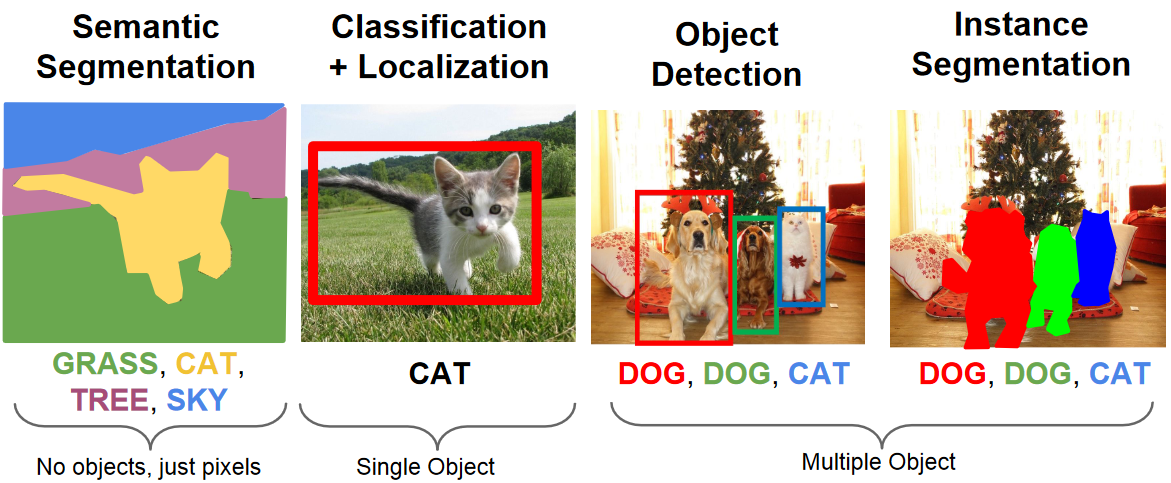
\includegraphics[width=0.8\textwidth]{Bilder/categories.png} 
	\caption{Verschiedene Aufgabenkategorien \cite{.10.11.2022}.}
	\label{fig:categories}
\end{figure} 

\section{Aktivierungsfunktionen} \label{sec:activation}

Im Folgenden wird der Stand der Technik für Aktivierungsfunktionen in \ac{ML}-Modellen dargelegt,
hierzu werden einige Funktionen kurz vorgestellt und deren Vor- und Nachteile bewertet. 
Die besprochenen Funktionen sind dargestellt in \autoref{fig:activation}.

\subsection{Sigmoid}

Die \textit{Sigmoid}-Funktion bildet die Eingabe auf einen Wert im Intervall $(0;1)$ ab und wird durch \autoref{eq:sigmoid} beschrieben.
Der Vorteil hier ist, dass Aktivierungen nie groß werden können, wodurch einzelne Neuronen nicht den Gradienten dominieren können und 
eine fortlaufende Normalisierung durchgeführt wird. Die Probleme hingegen sind, dass die Funktion eher aufwendig zu berechnen ist 
und dass die Ableitung für betragsmäßig größere Werte verschwindet. Hierdurch kann es zum \textit{Vanishing-Gradient-Problem} kommen, wobei 
Neuronen in den flacheren Schichten eines neuronalen Netzes kaum noch geupdated werden \cite{Goodfellow.2016} 
\begin{align}
	\label{eq:sigmoid} Sigmoid(z) = \frac{1}{1+e^{-z}}~.
\end{align} 

\subsection{\acf{ReLU}}

Die \textit{\acf{ReLU}} ist eine Aktivierungsfunktion, welche durch \autoref{eq:relu} ausgedrückt wird. 
\ac{ReLU} ist inzwischen der de-facto Standard von Aktivierungsfunktionen in den verborgenen Schichten eines Deep-Learning-Modells.
Dies liegt vor allem daran, dass das Vanishing-Gradient-Problem adressiert wird. Allerdings hat \ac{ReLU} das Problem, 
dass Neuronen auf $0$ gesetzt werden, wodurch sie kein Gradienten-Update mehr erhalten und dauerhaft genullt bleiben 
und somit nichts mehr zum Netzwerk beitragen - die Neuronen sterben. Das Problem wird \textit{Dying-\ac{ReLU}-Problem} genannt \cite{Goodfellow.2016} 
\begin{align}
	\label{eq:relu} ReLU(z) = \begin{cases} 
		z & z > 0 \\
		0 & z \leq 0 
	\end{cases}~.
\end{align} 

\ac{ReLU} erzielt eine höhere Inferenz- und Trainingsgeschwindigkeit bei gleicher oder besserer Performanz, 
als Sigmoid. Dies liegt zum einen an der Verbesserung des Vanishing-Gradient-Problems und zum anderen an der 
simpleren und damit leichter zu berechnenden Funktion \cite{Goodfellow.2016}.

\subsection{\acf{ELU}}

Die \textit{\acf{ELU}} ist eine Aktivierungsfunktion, die das Dying-\ac{ReLU}-Problem adressieren soll. 
Ausgedrückt wird die Funktion durch \autoref{eq:elu}. Die negative Komponente lässt zu, dass Neuronen nicht 
von einem Satz auf $0$ zurückkommen können, und weiterhin etwas zur Zielfunktion beitragen können. Außerdem ist die mittlere 
Aktivierung näher an $0$ als bei \ac{ReLU}, was zur Folge hat, dass das Training schneller konvergiert \cite{Clevert.23112015}
\begin{align}
	\label{eq:elu} ELU(z) = \begin{cases} 
		z & z > 0 \\
		\alpha \cdot (e^z - 1) & z \leq 0 
	\end{cases} ~.
\end{align}

Sowohl \ac{ReLU} als auch \ac{ELU} haben das Problem, dass Aktivierungen beliebig groß werden können, 
wodurch einige wenige Neuronen den Gradienten dominieren können, was zu langsamen Training und suboptimaler Performanz führen kann. 


\section{Ähnlichkeitsmaße} \label{sec:evaluation-metrics}

Im Folgenden sollen Ähnlichkeitsmaße zwischen Mengen, insbesondere 
solche, die als Kostenfunktion bzw. Bewertungsmetrik für einen binären 
Klassifikator verwendet werden können, untersucht werden. Hierzu wird zunächst Cross-Entropy betrachtet,
gefolgt von dem Dice- bzw. F-Maß. Weiter werden \ac{IoU} und das darauf aufbauende Quality-Maß betrachtet.

\subsection{\acf{BCE}}

Die \textit{Cross-Entropy} (bzw. dt. \textit{Kreuzentropie}) ist ein Maß des Unterschieds zweier
Wahrscheinlichkeitsdistributionen. Im Spezialfall einer binären Wahrscheinlichkeitsvariable 
kann die Cross-Entropy zur \textit{\acf{BCE}} spezialisiert werden, um auf ein binäres 
Klassifikationsproblem angewandt zu werden. 
\autoref{eq:bce} zeigt die Kalkulation von \ac{BCE}, wobei $p \in [0;1]$ die Prediction 
eines binären Klassifikators und $y \in \{0,1\}$ der Wert des Labels darstellen
\begin{align}
	\label{eq:bce} BCE = -[p \cdot \log(y) + (1-p) \cdot \log(1-y) ]~.
\end{align} 
Um über $n$ Prediction-Label-Paare $(p_i; y_i)$ den \ac{BCE} zu berechnen, wird das arithmetische Mittel nach
\autoref{eq:bce-mean} gebildet \cites{Cybenko.1999}{Murphy.2012}
\begin{align}
	\label{eq:bce-mean} BCE = -\frac{1}{n}\sum_{i = 1}^{n}[p_i \cdot \log(y_i) + (1-p_i) \cdot \log(1-y_i) ]~.
\end{align}

Im Sinne einer differenzierbaren Kostenfunktion im Kontext von \ac{ML} sind \ac{BCE},
\textit{negative Log-Likelihood} und \textit{Logistic-Regression} synonym \cite{Murphy.2012}. 

Aus \autoref{eq:bce-mean} geht hervor, warum \ac{BCE} gut geeignet für Klassifikationsprobleme ist.
Im Gegensatz zum mittleren absoluten Fehler, bei dem ein Fehler linear eingeht, und zum mittleren quadratischen Fehler,
bei dem ein Fehler quadratisch eingeht, geht ein Fehler bei \ac{BCE} exponentiell ein. 
Ein größerer Fehler wiegt also exponentiell stärker als ein kleinerer Fehler. 
Hierdurch werden die Fehler pro Datenpunkt und Klasse sehr klein, 
wodurch gute Performance und gute Generalisierung bei \ac{ML}-Modellen erreicht werden können. \\

Bei stark ungleichmäßiger Klassenverteilung kann es jedoch dazu kommen, 
dass die unterrepräsentierte Klasse kaum noch geschätzt wird, 
da der Fehler einer falsch geschätzten überrepräsentierten Klasse zu stark bestraft wird.
Dadurch lernt der Algorithmus, die unterrepräsentierte Klasse kaum zu schätzen.
Eine Abhilfe dagegen schafft eine Gewichtung der unterschiedlichen Klassen \cite{Ronneberger.18052015}.

\subsection{Dice- und F-Maß}

Das \textit{Dice-}, oder auch \textit{Sorensen-Dice-}Maß $D$ wurde 1945 bzw. 1948 erstmals vorgestellt und genutzt, um die Ähnlichkeit zweier botanischer Stichproben zu ermitteln. Verallgemeinert auf diskrete Mengen $X$, $Y$ kann deren Ähnlichkeit nach Dice $D$ beschrieben werden durch \autoref{eq:dice-coeff}. Es gilt $D \in [0; 1]$ \cites{Srenson.1948}{Dice.1945} 
\begin{align}
	\label{eq:dice-coeff} D = \frac{2 \cdot | X \cap Y |}{2 \cdot | X \cap Y | + |Y \setminus X| + |X \setminus Y|} 
	=\frac{2 \cdot | X \cap Y |}{|X| + |Y|} ~.
\end{align} 

Angewandt auf boolesche Mengen und binäre Klassifikatoren ist das Dice-Maß gleich dem $F_1$-Maß, das ein Maß für die Qualität eines statistischen Tests darstellt. Dafür sei $X$ nun die Menge der positiven Elemente und $Y$ die Menge der als positiv eingestuften Elemente. Dann ist die \textit{Genauigkeit} oder auch \textit{Precision} gegeben durch
\begin{align}
	\label{eq:precision} precision = \frac{|X \cap Y|}{|Y|}~,
\end{align}
der Anteil der richtig eingestuften Elemente an allen positiv eingestuften Elementen und die \textit{Trefferquote} oder auch \textit{Recall} gegeben durch
\begin{align}
	\label{eq:recall} recall = \frac{|X \cap Y|}{|X|}~,
\end{align}
der Anteil der richtig eingestuften Elemente an allen positiven Elementen. \\
Das F-Maß, bzw. genauer das $F_1$-Maß, ist dann gegeben durch das harmonische Mittel aus Precision und Recall, wobei $tp$ die Anzahl von wahr-positiven, $fp$ die Anzahl von falsch-positiven und $fn$ die Anzahl von falsch-negativen Elementen ist \cite{YutakaSasaki.2007}:
\begin{align}
	\label{eq:f1} F_{1} = \frac{2\cdot precision \cdot recall}{precision + recall} = \frac{2\cdot tp}{2 \cdot tp + fp + fn}~.
\end{align}
Precision und Recall können mit einem Faktor $\alpha$ unterschiedlich zueinander gewichtet werden, um mit $F_{\alpha}$ unterschiedliche Aspekte zu fokussieren. 

Das Dice-, bzw. $F_{\alpha}$-Maß kann leicht für eine differenzierbare Kostenfunktion genutzt werden mit Dice-Loss $D_{L}(X, Y) = 1 - D(X,Y)$, bzw. $F_{\alpha}$-Loss $F_{\alpha L}(X,Y) = 1 - F_{\alpha}(X,Y)$. 


\subsection{\acf{IoU}}

Die \textit{\acf{IoU}-} bzw. \textit{Jaccard-Ähnlichkeitsmetrik} ist ein weit verbreitetes Maß zur Bestimmung der Ähnlichkeit zwei diskreter Mengen. Hierzu seien $X$ und $Y$ diskrete Mengen. Dann ist die $IoU$ gegeben durch 
\begin{align}
	\label{eq:iou} IoU = \frac{|X\cap Y|}{|X \cup Y|} = \frac{| X \cap Y |}{| X \cap Y | + |Y \setminus X| + |X \setminus Y|}~.
\end{align} 
Für ein binäres Klassifikationsproblem lässt sich die $IoU$ ausdrücken durch 
\begin{align}
	\label{eq:iou-binary} IoU = \frac{tp}{tp + fp + fn}~,
\end{align}
wobei $tp$, $fp$, $fn$ wie in \autoref{eq:f1} \cite{Fletcher.2018}. 

Auffällig ist die Ähnlichkeit zum Dice- bzw. $F_{1}$-Maß. Es ist allerdings anzumerken, dass bei Dice/$F_1$ die $tp$, also die wahr-positiven, stärker gewichtet werden, als bei der \ac{IoU}. Die augenscheinliche Ähnlichkeit lässt sich durch die Beziehungen
\begin{align}
	\label{eq:dice-iou} IoU = \frac{D}{2 - D} \\
	D = \frac{2 \cdot IoU}{1 + IoU} ~,
\end{align}
beschreiben.
Im Gegensatz zur \ac{IoU} wird beim Dice-Maß eine höhere Gewichtung auf die wahr-positiven Elemente 
gelegt.

\subsection{Quality}

Bei der \textit{Quality} handelt es sich um eine gepufferte Form des \ac{IoU},
die toleranter bezüglich der Lokalität der Elemente der verglichenen Mengen, oder konkreter,
der Pixel einer semantischen Segmentierung, ist, 
wobei für dieselbe Eingabe $Quality \geq IoU$; $Quality \in [0;1]$ gilt, abhängig von der Puffergröße. 
Die Quality wird analog zur \ac{IoU} über eine gepufferte Precision - die \textit{Correctness} - 
und über einen gepufferten Recall - die \textit{Completeness} - berechnet. Insbesondere werden einige Elemente, 
die zuvor als $fp$ und $fn$ eingeordnet wurden, hiermit zu $tp$ konvertiert. \\
Die Quality soll einige Probleme der \ac{IoU} beheben, um ein Ähnlichkeitsmaß darzustellen, 
was näher an der praktischen und vom Menschen wahrgenommen Leistung eines \ac{ML}-Modells zur semantischen Segmentierung liegt.
So soll relativiert werden, dass vor allem im Randbereich einer Segmentierung einzelne abweichende Pixel
nicht als falsch anerkannt werden, sodass die Segmentierung im Großen und Ganzen als richtig anerkannt wird \cite{ChristianWiedemann.1998}. 

In dieser Arbeit für den Spezialfall von semantischer Segmentierung wird die Quality wie folgt berechnet: 
Sei $P$ die Prediction der Segmentierungsmaske für ein Eingabebild, $Y$ die tatsächliche Segmentierungsmaske (Ground-Truth / Label)
und $P, Y \in \{0, 1\}^{w \times h}$, wobei $w$ und $h$ die Breite und Höhe des Eingabebildes darstellen.
Die Einträge mit Wert eins von $P$ und $Y$ sind positiv, die Einträge mit Wert null negativ. Einträge repräsentieren Pixel.
$B$ sei die Puffergröße in Pixeln. \\
Zunächst sei die Hilfsfunktion $dilate_B: \{0,1\}^{w \times h} \mapsto \{0,1\}^{w \times h}$ definiert als 
\newcommand{\norm}[1]{\left\lVert#1\right\rVert}
\begin{align}
	\label{eq:dilate} dilate_B(A) = \left( \begin{cases} 
		1 & \exists a_{kl} \in A: a_{kl} = 1 \land \norm{
			\begin{pmatrix} k \\ l \end{pmatrix} - \begin{pmatrix} i \\ j \end{pmatrix} }_2 \leq B \\
		0 & else 
	\end{cases} \right)_{ij}~.
\end{align}
Die Funktion $dilate_B$ bildet eine Matrix auf eine weitere derselben Ordnung ab, 
sodass alle Einträge gleich eins sind, die in der Eingabematrix eins sind. Zusätzlich sind alle Einträge eins, 
die im Umkreis von $B$ Pixel um eine Eins in der Eingabematrix liegen. Somit werden die positiven 
Pixel der Eingabematrix um die Bufferzone erweitert.  \\
Damit lassen sich die gepufferten, fehlertoleranteren wahr-positiv $tp_B$, falsch-positiv $fp_B$ und 
falsch-negativ $fn_B$ Werte berechnen: 
\begin{align}
	\label{eq:buffering} {tp}_B = \norm{dilate_{B}(Y) \odot P}_{1,1} , \\
	fn_B = \norm{Y - (Y \odot dilate_{B}(P))}_{1,1} , \\
	{fp}_B = \norm{P}_{1,1} - {tp}_B .
\end{align}
Beispielhaft und intuitiv dargestellt für $tp_B$: Es sollen auch alle Eins-Pixel als wahr-positiv aufgefasst werden,
die leicht von der Ground-Truth abweichen, also sich noch in der Pufferzone befinden. 
Hierfür wird die Pufferzone um die Ground-Truth $Y$ gelegt und das Hadamard-Produkt mit der Predicition $P$ gebildet.
Da alle Matritzen als Einträge nur 0 oder 1 enthalten, findet durch das Hadamard-Produkt eine Art Verundung statt, 
sodass im Produkt nur Einträge eins sind, die in beiden Matritzen eins sind. Der Rest ist null. 
Durch die zuvor durchgeführte Pufferung mit $dilate_B$ sind allerdings auch Einträge gleich eins, die in $Y$ 
zuvor null waren. Hierdurch besitzt das Hadamard-Produkt mehr Einträge mit eins, als bei der Berechnung der \ac{IoU}.
Diese Zahl ist genau um die Anzahl an positiven Pixeln aus $P$ größer, die in der Pufferzone liegen. 
Schließlich wird mit der $1,1$-Höldernorm für Matritzen die Anzahl an Einsen gezählt, was dann $tp_B$ ergibt. \\
Die Formel für die Quality ist analog zur \ac{IoU}, bis auf die Verwendung der jeweils gepufferten Variablen:
\footnote{\autoref{code:quality} zeigt die dazugehörige Python-Implementation.}
\begin{align}
	\label{eq:quality} quality = \frac{tp_B}{tp_B + fp_B + fn_B} ~.
\end{align}

\section{Architekturkomponenten}

Im Folgenden werden verschiedene Architekturkomponenten diskutiert, die im \ac{ML} allgemein 
bzw. bei semantischer Segmentierung im Speziellen verwendet werden. Hierzu werden zunächst Dropout-Layer 
und Batch-Normalization-Layer begutachtet und dann die U-Net-Architektur zur semantischen Segmentierung vorgestellt. 

\subsection{Dropout} \label{sec:architekturkomponenten:dropout}

\textit{Dropout} ist eine ressourcenschonende Regularisierungstechnik für \ac{ML}-Modelle. 
Hierbei werden einzelne Neuronen mit einer Wahrscheinlichkeit von \textit{Rate} $r$ während des Trainings 
deaktiviert, also deren Output auf $0$ gesetzt.\\ 
Da bei der Inferenz Dropout dazu führen kann, 
dass wichtige Features ignoriert werden, ist Dropout während der Inferenz unerwünscht. Ohne Dropout während der 
Inferenz sind allerdings alle Gewichte aktiv, was zu einer höheren Summe der Gewichte während der Inferenz, 
als während des Trainings führt. Deswegen müssen die Gewichte für die Inferenz nach unten skaliert werden. 
Alternativ können während des Trainings alle Gewichte nach oben skaliert werden, die nicht deaktiviert wurden. 
Somit muss für die Inferenz keine Anpassung vorgenommen werden. Nach jedem Trainings-Batch werden die aktivierten 
Neuronen dann um Faktor $\frac{1}{1-r}$ skaliert \cites{Goodfellow.2016}{NitishSrivastava.2014}.

Es hat sich gezeigt, dass Dropout eine effektivere Regularisierungstechnik zur Minderung von Overfitting ist, 
als andere ressourcenschonende Techniken, wie \textit{Weight-Decay}, \textit{Filter-Norm-Constraints} oder 
\textit{Sparse-Activity-Regularization}, wobei Dropout mit diesen kombiniert werden kann, für noch bessere 
Regularisierung \cites{Goodfellow.2016}.

\subsection{Batch-Normalization} \label{sec:architekturkomponenten:batchnorm}

\textit{Batch-Normalization} normalisiert und standardisiert den Output von Neuronen auf Basis des Mittelwerts 
und der Streuung einer Batch während des Trainings. Für die Inferenz werden Durchschnittswerte 
des Mittelwerts und der Streuung der Batches des Trainingsdatensatzes herangezogen und angewandt. \\
Batch-Normalization führt zu einer schnelleren Konvergenz im Training, 
sodass die Anzahl an benötigten Epochen in manchen Fällen bis zu halbiert werden können. Des Weiteren führt 
Batch-Normalization zu einer gewissen Regularisierung, da es die Kostenfunktion zu einem gewissen Grad glättet 
\cites{Goodfellow.2016}{Ioffe.11022015}.
Besonders gut funktioniert Batch-Normalization für \acp{CNN} und Netzwerke mit Sigmoid-Aktivierungsfunktion
\cites{Goodfellow.2016}.

\subsection{U-Net} \label{sec:architekturkomponenten:unet}

Die \textit{U-Net-Architektur} beschreibt eine \textit{Fully-Convolutional-Network-Architektur}, die erstmals in Freiburg 2015 vorgestellt wurde 
und herausragende Ergebnisse für verschiedene Benchmarks, insbesondere zur semantischen Segmentierung kleiner Datensätze, liefert. \\
Aus \autoref{fig:u-net-architecture} geht die namensgebende Architektur der U-Net hervor. Die folgenden Besonderheiten 
führen zu der sehr guten Performanz des Netzes bei semantischer Segmentierung \cite{Ronneberger.18052015}:
\begin{itemize}
	\item Das Netz besteht aus einem kontrahierenden Encoder-Teil (linke Hälfte) und einem expandierenden und symmetrisch aufgebauten
	Decoder-Teil (rechte Hälfte). Der Encoder erzeugt feinere \textit{Feature-Maps} mit zunehmender Netztiefe, 
	während der Decoder diese wieder extrapoliert, was zu einer besseren Lokalisierung führt. 
	\item Zwischen den jeweiligen symmetrischen Encoder- bzw. Decoder-Blöcken befinden sich \textit{Skip-Connections}\footnote{\textit{copy and crop} in der Abbildung.}.
	Zusammen mit dem vorherigen Punkt erhöht dies weiter die Lokalisierung und Performanz, da der jeweilige Decoder-Block feinere Features von der \textit{Up-Convolution}\footnote{implementiert als \textit{Transposed Convolutions}.},
	wie auch den größeren Kontext von früheren Blocks mittels Skip-Connection erhält. 
	\item Zur Mitte des Netzes hin erhöht sich die Anzahl der Convolution-Filter und damit die Anzahl der \textit{Channel}, 
	während sich die Dimensionen der einzelnen Feature-Maps durch das \textit{Downsampling} verringert. 
	Hierbei ist anzumerken, dass bei der Implementation kein \textit{Padding} für die Convolutions verwendet wurde,
	wodurch sich die Dimensionen der Feature-Maps nach jeder Convolution verringert. 
	Hieraus folgt ein Zuschneiden für die Skip-Connections. 
\end{itemize}

\begin{figure}
	\centering
	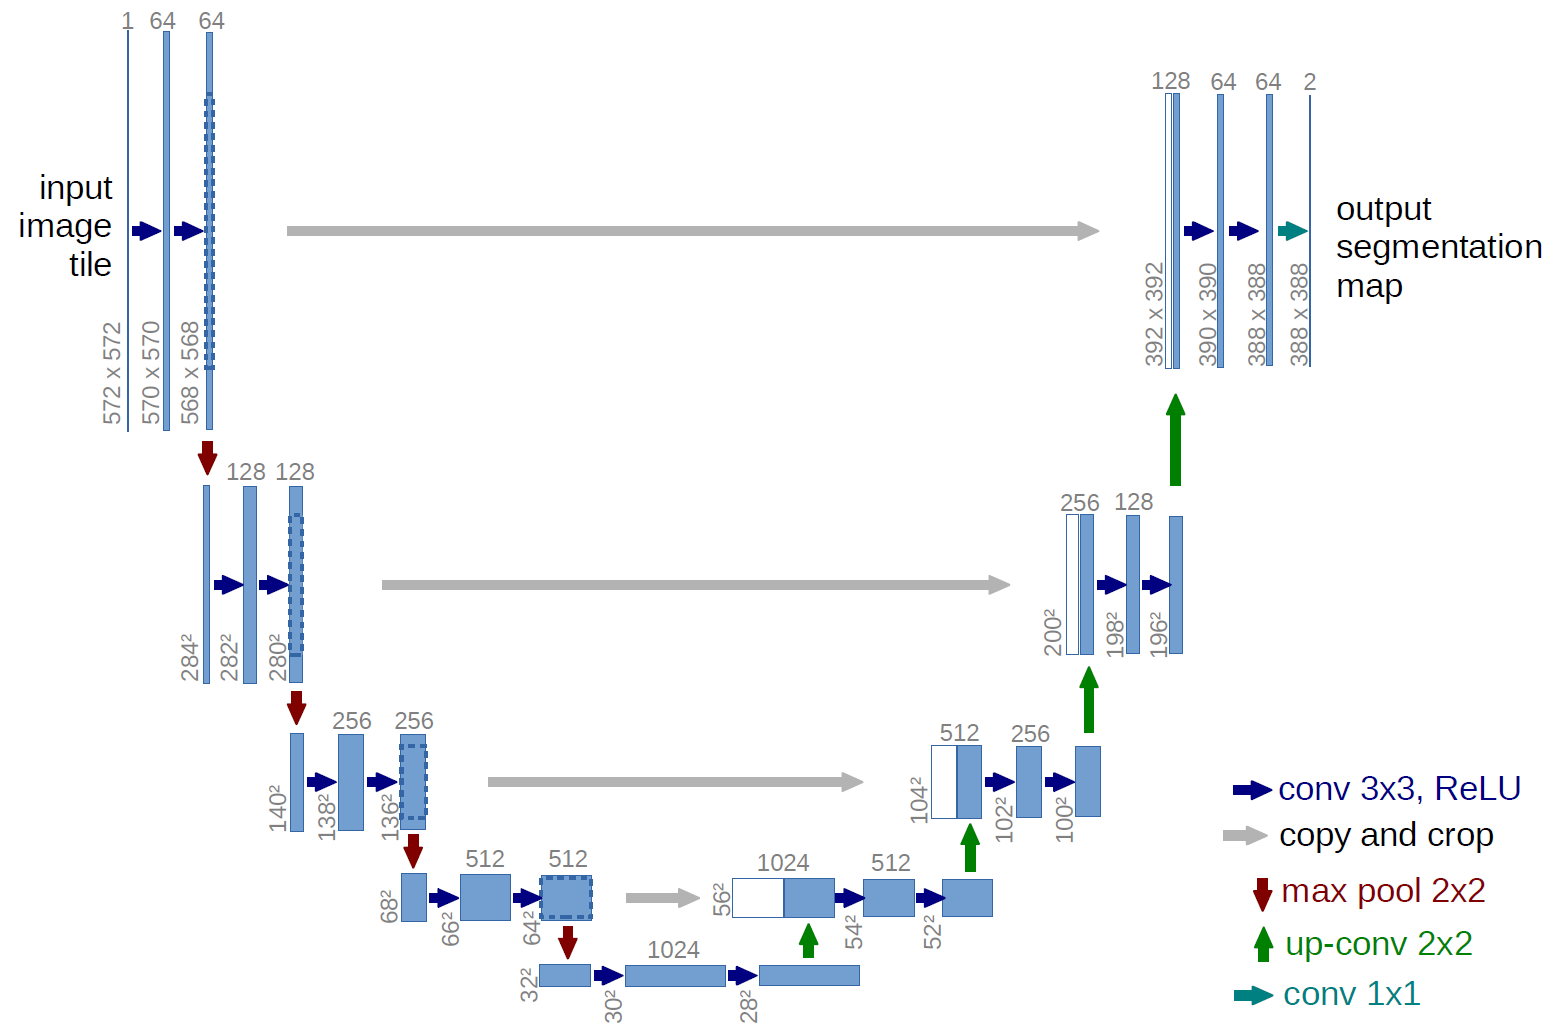
\includegraphics[width=0.8\textwidth]{Bilder/u-net-architecture.png} 
	\caption{Ursprüngliche U-Net-Architektur \cite{Ronneberger.18052015}.}
	\label{fig:u-net-architecture}
\end{figure} 


\section{Vortrainierte \ac{CNN}-Modelle} \label{sec:pretrained-backbones}

Im Folgenden wird eine Auswahl an \ac{CNN}-Modellen vorgestellt, von denen es öffentlich zugängliche,
vortrainierte Instanzen zur freien Verwendung gibt. Diese können zu Transfer-Learning-Zwecken 
genutzt werden, indem sie zum Beispiel als Teilnetz in eine \ac{CNN}-Architektur eingebaut werden 
(mehr dazu in \autoref{sec:transfer-learning}). \\ 
Die Klassifikations-Modelle sind auf dem Bildklassifikationsdatensatz \textit{ImageNet}, der über 14 Mio. Bilder 
mit 1000 Objektklassen enthält, trainiert. Der ImageNet-Datensatz ist der größte und bekannteste 
Datensatz seiner Art und ist sehr beliebt für Benchmarks und Pre-Training.

\subsection{VGG16} \label{sec:pretrained-backbones:vgg16}

\textit{VGG16} ist ein \ac{CNN}, welches 2015 von der \textit{Visual Geometry Group} vorgestellt wurde 
und zu der Zeit bahnbrechende Ergebnisse bei der Bilderklassifizierung lieferte \cite{Simonyan.04092014}. 
Inzwischen ist es ein Standard-Netz, auf welchem viele weitere Architekturen aufbauen,
um verschiedene Verbesserungen zu realisieren. 
Dadurch ist es auch sehr beliebt für Transfer-Learning. 

VGG16 besteht aus fünf Blöcken mit $3x3$-Convolution-Schichten,
gefolgt von drei Fully-Connected-Schichten. Die ersten beiden Convolution-Blöcke haben zwei Convolution-Schichten,
die letzten drei Blöcke dagegen jeweils drei. 
Jeder Convolution-Block wird gefolgt von einer Maxpool-Schicht und jeder bis auf den vorletzeten verdoppelt die Filteranzahl in den Convolution-Schichten,
beginnend bei 64 Filtern im ersten Block bis hin zu 512 Filtern in den letzten beiden Blöcken \cite{Simonyan.04092014}\footnote{\autoref{fig:vgg16-architecture} veranschaulicht VGG16.}. 

Das gesamte Netz besitzt 138 Mio. Parameter. Werden die drei Fully-Conntected-Schichten am Ende ausgelassen, 
sind es ungefähr 14,7 Mio. Parameter. 

\subsection{ResNet34} \label{sec:pretrained-backbones:resnet}

Damit Modelle mehr und feinere Features lernen können, müssen sie in der Lage sein, sehr komplexe Funktionen darzustellen. 
Das führt dazu, dass tiefere Netze auf dem ImageNet-Datensatz tendenziell bessere Ergebnisse erzeugen, als flachere. 
Hierin lag auch der Erfolg von VGG16 bzw. VGG19. Jedoch führt das einfache Vertiefen von Netzen zu dem Degredation-Problem, wonach 
flachere Netze besser performen, als tiefere, da die tieferen sehr schwer zu trainieren sind. \\
Dieses Problem adressiert \textit{ResNet} erfolgreich, indem \textit{Residual-Blocks} eingeführt werden. 
Hierdurch können mit \textit{ResNet} tiefere Netze erstellt werden als bisher, die trotzdem noch effizient trainiert werden können.
Ein Residual-Block besteht dabei aus zwei Convolutional-Layer mit einer Skip-Connection zwischen Input der ersten Layer und Output 
der zweiten Layer. Durch die Skip-Connections kann bei der Backpropagation der Gradient ungehindert rückwärts laufen, 
um so auch die flachen Layer upzudaten. So kann z.B. \textit{ResNet34} 34 trainierbare Layer haben, 
während zuvor mit VGG nur 16 bzw. 19 effektiv waren \cite{He.10122015}. 

Die Architektur ist dabei sehr simpel. Sie stellt - im Falle von ResNet34 - im Prinzip 33 Convolutional-Layer mit wiederholtem Downsampling 
und Skip-Connections zw. jeweils zwei Convoltuional-Layern, gefolgt von einer Fully-Connected-Layer dar \cite{He.10122015}\footnote{\autoref{fig:resnet34-architecture} veranschaulicht ResNet34.}.

ResNet34 hat 63,5 Mio. Parameter. Wird auf die letzte Fully-Connected-Layer verzichtet, sind es 21,2 Mio. Parameter.


\subsection{DenseNet121} \label{sec:pretrained-backbones:densenet121}

\textit{DenseNet121} wurde 2018 erstmals vorgeschlagen und wurde designed, um das Vanishing-Gradient-Problem 
zu verbessern, bessere Feature-Übertragung in tiefere Netzschichten zu ermöglichen und das Wiederverwenden von Features 
zu unterstützen, um somit die Anzahl der benötigten Parameter deutlich zu reduzieren, bei gleichbleibender Performanz \cite{Huang.25082016}.

Das Netz besteht aus mehreren sogenannten Dense-Blöcke, die wie folgt aufgebaut sind: 
Jede angegebene Convolution-Schicht besteht aus einer Batch-Normalization-Schicht mit \ac{ReLU}-Aktivierung,
gefolgt von der angegebenen Convoltuion-Schicht. Außerdem - und hier liegt die große Erweiterung des DenseNet - sind alle 
Convolution-Schichten eines Dense-Blocks mit allen nachfolgenden Convolution-Schichten des Dense-Blocks konkateniert,
anstatt nur mit dem einen Nachfolgenden, wie es zum Beispiel bei VGG16 der Fall ist\footnote{\autoref{fig:densenet121-architecture} veranschaulicht DenseNet121.}. 

DenseNet121 enthält circa 7,6 Mio. Parameter. Ohne die letzte Fully-Connected-Schicht sind es noch circa 6,9 Mio. 
Bei nur halb so vielen Parametern erreicht DenseNet121 leicht bessere Ergebnisse als VGG16 auf dem ImageNet-Datensatz 
(93\% ggü. 92\% Accuracy für ImageNet-Top5) \cite{Huang.25082016}. 


\section{Transfer-Learning mit U-Net} \label{sec:transfer-learning}

\textit{Transfer-Learning} beschreibt das Übertragen von trainierten Gewichten eines \ac{ML}-Modells auf ein anderes, 
bestenfalls ähnliches Problem und Modell. Das Modell wird dann via \textit{Fine-Tuning} verfeinert mit dem neuen Datensatz und unterschiedlichen Trainingsmethoden.
Häufig wird dafür ein Teil des Modells eingefroren, sodass sich die eingefrorenen Gewichte nicht verändern können. Dies verhindert, 
dass die bereits vortrainierten Gewichte durch die erste Trainings-Batch ruiniert und unbrauchbar werden. Eine weitere Möglichkeit ist,
mit einer sehr geringen Lernrate das gesamte Modell zu trainieren. Oft werden beide Ansätze auch verbunden.

Der Vorteil von Transfer-Learning liegt darin, dass das Training deutlich kürzer dauert, 
weil direkt mit einer höheren Genauigkeit eingestiegen wird, mit kleineren Datensätze bessere Ergebnisse erzielt werden können
 und auch insgesamt eine höhere Genauigkeit 
am Ende des Trainings erreicht wird, als bei herkömmlichem Training. Diese Effekte sind verstärkt, 
abhängig davon, wie ähnlich der Datensatz des Pre-Trainings und des eigentlichen Trainings sind \cite{Ruder.3212017}. \\
Insbesondere bei Computer-Vision ist Transfer-Learning effektiv, da bei Bildern high-level Features wie Clustering 
ähnlichfarbener Pixel oder Kantenerkennung oftmals sehr ähnlich zwischen unterschiedlichen Datensätzen ausfallen 
und damit schon vorhanden sind \cite{Ruder.3212017}. 

Für Transfer-Learning mit U-Nets gibt es verschiedene Strategien: Backbone-Netze als Encoder, 
partielles Einfrieren verschiedener Netzbereiche und direktes Trainieren mit geringer Learning-Rate.
Der Stand der Wissenschaft diesbezüglich wird im Folgenden vorgestellt. 

\subsection{Training mit Backbones} \label{sec:transfer-learning:backbones}

Im Kontext von Transfer-Learning bei U-Nets bezeichnet ein \textit{Backbone} ein etabliertes vortrainiertes \ac{CNN}, 
welches, leicht modifiziert, als Encoder für das U-Net verwendet wird. Hierbei wird der Decoder-Teil des U-Net 
symmetrisch dem Encoder nachempfunden und an passenden Stellen Skip-Verbindungen zwischen En- und Decoder eingebaut. \\
Hierdurch kann eine geeignete \ac{CNN}-Architektur für das spezifische Problem ausgewählt werden. Des Weiteren sind diese 
Modelle auf sehr großen Datensätzen, wie \textit{ImageNet}, vortrainiert öffentlich zugänglich. 

Bei der semantischen Segmentierung von medizinischen Lungen-Ultraschall-Bildern, wurden die besten Ergebnisse von einem Dice-Maß-Standpunkt aus, 
mit einem U-Net mit auf ImageNet trainierten \textit{VGG16}-Backbone erzielt. Das Vergleichsnetz, welches zuerst auf dem \textit{Salien Object}
Datensatz vortrainiert wurde, erzielte schlechtere Ergebnisse von dem Dice-Maß her, wobei allerdings das VGG16-U-Net kleine falsch-positive 
Regionen erkannte, die weit außerhalb der Ground-Truth lagen. Die falsch-positiven beim Vergleichsnetz, lagen direkt an der Ground-Truth, 
dies lässt auf eine sensitivere Kantenerkennung beim VGG16-U-Net schließen, die manchmal aber auch übersensitiv war \cite{Cheng.05.10.2021}. 

Für das Training des VGG16-U-Nets wurde der Encoder-Teil eingefroren und somit nur der Decoder trainiert. 

\subsection{Partielles Einfrieren und Training mit geringer Lernrate}

Im oben beschriebenen Problem zur semantischen Segmentierung wurde das vortrainierte Vergleichsnetz auf zwei Weisen fein-trainiert:
\begin{enumerate}
	\item Ohne Einfrieren mit einer Lernrate von $10^{-5}$
	\item und mit Einfrieren des mittleren Blocks, welcher ungefähr $14\cdot 10^6$ der insgesamt $31 \cdot 10^6$ Parameter enthielt. 
\end{enumerate}
Die 5-fache Kreuzvalidierung ergab sowohl für den besten Lauf, als auch für den durchschnittlichen Lauf, ein besseres Dice-Maß 
für das Training aller Parameter. In keinem der Fälle gab es, anders als beim VGG16-U-Net, segmentierte Regionen ohne Zusammenhang mit der Ground-Truth \cite{Cheng.05.10.2021}. 

In einem weiteren Paper wurde untersucht, welche Layer eines U-Net am besten eingefroren werden sollten, für das Fine-Tuning von medizinischen Bildern - 
zum einen von Lungen-Ultraschall-Bildern und zum anderen von Brust-Röntgen-Aufnahmen. 
Hier wurde wieder mit dem \textit{Salien Objetcs} Datensatz vortrainiert. Dann wurden für beide Anwendungsfälle folgende Tests durchgeführt: 
\begin{enumerate}
	\item Einfrieren der linken Hälfte (Encoder) des Netzes,
	\item Einfrieren der rechten Hälfte (Decoder) des Netzes,
	\item gesamtes Netz, bis auf den ersten Block eingefroren und dann nach jeweils fünf Epochen sukkzessive weitere Blöcke freigeben und
	\item dasselbe allerdings von hinten nach vorne.
\end{enumerate}
Für die Röntgenaufnahmen gab es keine Unterschiede, wobei der Dice-Score hier allerdings auch bei $0.98$ lag. 
Für die Ultraschallbilder lieferte Methode (1) die schlechtesten Ergebnisse (Dice: $0.72$), gefolgt von Methode (2) (Dice: $0.80$) 
und gleichermaßen (3) und (4) (Dice: $0.82$), wobei (3) deutlich schneller konvergierte \cite{Amiri.19.02.2020}. \\ 
Es ist ersichtlich, dass die Methodik beim Fine-Tuning, abhängig vom Datensatz, einen erheblichen Einfluss 
auf die abschließende Performanz des Modells haben kann und stets berücksichtigt und gegen Alternativen abgewogen werden sollte,
um beste Ergebnisse zu erzielen. Die vorgestellten Methodiken können später genutzt werden, 
um eine Transfer-Learning-Methode für das Problem der Radwegerkennung zu konzipieren. 


\section{Aktueller Stand bei der Straßendetektion}

Die Erkennung von Fahrradwegen soll auf der bereits existierenden Straßenextraktion aus Satellitenbildern aufbauen.
Hierfür werden vorhandene Datensätze für Straßen vorgestellt. 
Im Anschluss werden auf den aktuellen Stand und Benchmark-Optionen eingegangen.

\subsection{Datensätze} \label{sec:road-detection:roads-data}

Im Folgenden sind alle relevanten Datensätze zur Straßenerkennung aus Luftbildern aufgeführt. 
Eine Auswahl der später zum Pre-Training verwendeten Datensätze findet im \autoref{sec:pre-training-roads} statt.\\
Ein Testdatensatz ist hierbei ein meist sehr kleiner Datensatz, der ausschließlich zum Testen und Bewerten eines bereits 
trainierten Modells verwendet werden soll. Im Rahmen der Straßenerkennung ist dies besonders relevant, 
da sich unterschiedliche Städte in unterschiedlichen Ländern und Kulturen stark unterscheiden können, 
während die Trainingsdaten meist nur aus einer Stadt, die in sich ein eher homogenes Bild aufweist, bestehen.
Der Testdatensatz soll also die Generalisierungsfähigkeit des Netzes testen, um zu sehen,
ob das Modell, das bspw. auf einem Datensatz einer modernen amerikanischen Stadt trainiert wurde, 
auch auf Bildern einer mitteleuropäischen Altstadt funktioniert. Deswegen ist es wichtig, 
dass keine Bilder des Testdatensatzes im Training verwendet werden. 

% Bei den letzten Datensets zu Toronto, Vaihingent und Potsdam handelt es sich um Testdatensätze. 
Beim \textit{Massachusetts Roads Dataset} liegen $1171$ Luftaufnahmen aus dem Gebiet Massachusetts vor.
Jedes der Bilder besteht aus $1500\times 1500$ Pixeln, was einer Fläche von $2.25 km^2$ entspricht.
Die gesamte Abdeckung sind $2600 km^2$ bestehend aus städtischer und ländlicher Gegend.
Der Split erfolgt im Verhältnis $95:1:4$. 
Über den Split wird sichergestellt, dass keine Durchmischung der Test- und Validierungsdaten mit den Trainingsdaten erfolgt und die Bewertung des Netzes verfälscht wird.
Es gibt also $1108$ Trainings-, $14$ Validierungs- und $49$ Testbilder.
Die Zielbilder sind über eine Rasterung der Straßenmittellinien aus dem \ac{OSM}-Projekt generiert worden.
Die Liniendicke der gelabelten Straßen beträgt $7 px$ und ist ungeglättet, da hiermit bessere Ergebnisse erzielt worden sind \cite{.06.04.2014}.
Der Zuschnitt der Bilder sorgt teilweise für einen hohen Anteil weißer Stellen in den Bildern.

Das \textit{Buffalo Roads Dataset} ist als zusätzliches Testset für das Massachusetts Roads Dataset zu sehen.
Hintergrund ist die Überprüfung des Netzes mit Daten aus einem anderem Gebiet unter anderen Bedingungen.
Es besteht lediglich aus 30 Orthophotos ($5:5:20$) mit einer Größe von $609\times 914$ und einer Auflösung von $1 \frac{px}{m^2}$.
Die Generierung der gelabelten Daten erfolgt analog zum Massachusetts Road Set über \ac{OSM}.
Größter Unterschied ist die Verdeckung von Straßen durch Bäume \cite[86-88]{.06.04.2014}.

\textit{LandCover.ai} kann für die Erkennung von Gebäuden, Waldgebieten, Gewässern und Straßen verwendet werden.
Die Aufnahmen stammen aus Polen und Zentraleuropa in einer Größe von $21627 km^2$.
$33$ Orthophotos haben eine Auflösung von $25 \frac{cm}{px}$ mit $9000\times 9500$ Pixeln, $8$ Bilder von $50 \frac{cm}{px}$ mit $4200 \times 4700$ Pixeln \cite{.20.04.2022}.
Die Bilder sind hand-annotiert und beinhalten einen großen Anteil an ländlichen Gebieten.

Mithilfe des \textit{Deep Globe Road Extraction Datasets} können in Kathastrophgebieten Informationen über Karten und Zugänglichkeitsmöglichkeiten für die Krisenbewältigung gesammelt werden.
Der Datensatz besteht aus $6226$ Satellitenbildern in RGB mit einer Größe von $1024\times 1024$.
Die Auflösung der Aufnahmen beträgt $50 cm$.
Mit $1243$ Validierungs- und $1101$ Testdaten ist der Split in Training, Validierung und Test zu $73:15:13$ erfolgt.
Der hohe Aufwand zur Erstellung der Labels führt zu Ungenauigkeiten, insbesondere in ländlichen Regionen. 
Kleine Straßen innerhalb von Landwirtschaftsflächen sind bewusst unbeschriftet geblieben.
Die Bilder sind ursprünglich über Thailand, Indonesien und Indien mit je $19584\times 19584$ Pixeln aufgenommen worden.
Insgesamt entspricht es einer Fläche von $2220 km^2$ \cite{Ashwath.10.11.2020}.

Mit finanzieller Unterstützung des Chesapeak Bay Programms wurde ein Datensatz \textit{Land Cover} zur Landnutzung und Bodenbedeckung erstellt.
Es lassen sich Einblicke in die Landschaft und die Verwaltung der Regionen gewinnen.
Das Einzugsgebiet umfasst $250.000km^2$ mit einer Auflösung von $1m$. 
Damit handelt es sich bei diesem Datensatz um den größten bei der Analyse von der Landnutzung im Vergleich zur Bodenbedeckung \cite{ChesapeakeConservancy.02.06.2022}.

Bei den nachfolgenden drei Datensätzen handelt es sich um Testdatensätze.
Das \textit{Toronto Dataset} umfasst $1,45km^2$ im Umkreis der Stadt Toronto in Canada. 
Darin enthalten sind ca. $1 km$ Straßen mit einer Bodenauflösung von $15cm$. 
Zusätzlich werden Laserscanner mit $6 \frac{points}{m^2}$ bereitgestellt.
Im Datensatz ist eine hohe Varianz bezüglich der Gebäudehöhe, Struktur der Dächer und verschiedener Straßen vorzufinden.
Der Testbestand kann für die Überprüfung von Objektextraktion und Gebäuderekonstruktionstechniken in zwei weitere Teilgebiete unterteilt werden.
Für Straßen können alle Testdaten verwendet werden.
Die Labels sind manuell mithilfe von CloudCompare erstellt worden \cite{Englich.06.10.2022b,Tan.2020}.

Der Testdatensatz \textit{Vaihingen/Enz} besteht aus einer Untermenge der Daten, welche für einen Test von digitalen Luftbildkameras verwendet wurden.
Er ist in drei Testgebiete für verschiedene Objektklassen und in einen größeren Bereich für das Überprüfen von Straßenextrakion aufgeteilt, wobei die drei Gebiete hier mit inbegriffen sind.
Die einzelnen Gebiete sind in verschiedene Kategorien unterteilt: Hochhäuser, Wohngebiete mit kleineren Einfamilienhäusern und Innenstadt mit dichter Bebauung.
Die Bodenauflösung beträgt $8cm$ \cite{Englich.06.10.2022b}.

Für die Stadt \textit{Potsdam} gibt es einen ähnlichen Datensatz. 
Dieser zeigt eine typsiche Altstadt mit großen Gebäudeblöcken, kleinen Straßen und einer dichten Besiedelung.
Die \ac{GSD} beträgt $5cm$.
Zur Vermeidung von Randbereichen ohne Daten, sind zentrale Ausschnitte verwendet worden.
Übrig gebliebene Datenlücken wurden interpoliert \cite{Englich.17.11.2022, Englich.17.11.2022b}.

\subsection{Aktueller Stand und Benchmarks} \label{sec:state-of-the-art-roads} % ...der straßen detection

Die aktuellen State-Of-The-Art-Methoden zur Extraktion von Straßen aus Satelliten- und Luftbildern verwenden 
alle Computer-Vision mittels \acp{CNN} und dabei ausschließlich Netze aus der U-Net-Familie - also angepasste, 
erweiterte, abgeänderte U-Nets \cites{C.Henry.2021, Constantin.2018, Kamiya.2018, Yerram.2022}. \\
Dies liegt vor allem daran, dass das U-Net, welches ursprünglich für biomedizinische Bilder entworfen wurde, 
genau die Probleme adressiert, die auch beim Segmentieren von Straßen auf Luftbildern auftreten. 
Wie auch in medizinischen Bildern leiden die Luftbilder-Datensätze häufig unter großer Klassen-Imbalance 
und unter ähnlichen Annotationsfehlern. Außerdem haben viele medizinische Bilder und Luftbildaufnahmen von Straßen 
ähnliche Topologien. Komplexere Architekturen zur semantischen Segmentierung, wie zum Beispiel solche 
für Bodenaufnahmen-Datensätze (vgl. KITTI \cite{Geiger.2013}) erreichen nicht die Performance von U-Nets bei 
Luftbild-Benchmarks \cite{C.Henry.2021}. \\
Weiter wird die Extraktion von Straßen aus Satelliten- bzw. Luftbildern zumeist in zwei Phasen eingeteilt: 
\begin{enumerate}
	\item das Erstellen einer binären Maske zu den Luftbildern mittels semantischer Segmentierung, 
	welche die Straßen pixelweise induziert, 
	\item das Extrahieren eines topologischen Graphens, welcher die Straßen-Zentrumslinien beschreibt.   
\end{enumerate}
Schritt (1) wird dabei zumeist von U-Net-Derivaten behandelt, wobei es allerdings auch Vorschläge von Netzen gibt, 
die direkt Schritt (2) ausführen \cite{C.Henry.2021}.
Im Folgenden wird weiter Schritt (1) betrachtet.   

Der Vergleich von unterschiedlichen Netzen, Papern und Ergebnissen zur Straßenerkennung ist häufig erschwert, 
da es trotz gleicher Bewertungsmaße wie Dice oder \ac{IoU}, zwei unterschiedliche gängige Kodierungen gibt:
\begin{enumerate}
	\item Das verwendete \ac{CNN} hat je Input-Neuron bzw. -Pixel $p$ genau ein Output-Neuron $o_p$, welches den jeweiligen Input-Pixel $p$
	als Straße identifiziert, genau dann, wenn der Wert des Output-Neuron $o_p$ einen gewissen Grenzwert $l$ überschreitet ($o_p > l$), 
	ansonsten ($o_p \leq l$) gilt der Pixel $p$ \textit{implizit} als Nicht-Straße, bzw. \textit{Hintergrund}. \\
	In diesem Fall stellt ein korrekt als Hintergrund klassifizierter Pixel ein wahr-negatives Ergebnis dar. 
	Wahr-Negative werden von Dice, bzw. \ac{IoU} allerdings nicht berücksichtigt (vgl. \autoref{eq:f1} und \ref{eq:iou-binary}).
	Ein so klassifizierter Pixel ändert also nichts an dem Score. Es werden nur Straßen betrachtet, nicht aber der Hintergrund.    
	\item Das verwendete \ac{CNN} hat je Input-Neuron bzw. -Pixel $p$ \textit{zwei} Output-Neuronen $\mathbf{o_p} = (o_{p_S}, o_{p_H})$, 
	wobei dies eine One-Hot-Kodierung von Punkt (1) darstellt. 
	Ein Hintergrund-Pixel wird nun \textit{explizit} als solcher klassifiziert. 
	Dies ändert allerdings die Berechnungsgrundlage von Dice und \ac{IoU} erheblich, da diese nun (zumeist) als Mittelwert 
	der Scores zu $o_p{_S}$ und $o_p{_H}$ berechnet werden. Hierdurch fließen die zuvor unberücksichtigten wahr-negativen 
	Hintergrundpixel als wahr-postive in den Dice- bzw. \ac{IoU}-Score ein. Die Verzerrung wird noch verstärkt, 
	da eine starke Imbalance zwischen Straßen- und Hintergrundpixel herrscht, wodurch der Dice-/\ac{IoU}-Score bei 
	der One-Hot-Kodierung viel mehr eine Aussage darüber trifft, wie viele Hintergrundpixel, von denen es ja viel mehr gibt,
	richtig klassifiziert wurden. Die so erzielten Dice-/IoU-Werte sind hier rein numerisch deutlich höher. 
\end{enumerate}

Im Weiteren werden aktuelle Ergebnisse zu den Massachusetts- und Deep-Globe-Datensätzen vorgestellt, 
um zu Ermitteln, was für diese Datensätze gut funktioniert, sodass diese state-of-the-art Erkenntnisse beim 
späteren Entwurf eines oder mehrerer Netze zum Erkennen von Fahrradwegen (s. \autoref{sec:architecture}) 
genutzt werden können. Die beiden Datensätze sind für die Literaturrecherche ausgewählt, 
da sie sehr häufig als Benchmark zum Erkennen von Straßen genutzt werden, es dazu sehr viel Literatur und 
Forschung gibt und da beide Datensätze sich stark unterscheiden, soweit das im Rahmen der Straßenerkennung möglich ist. 
Haben die State-Of-The-Art-Lösungen trotz des starken Unterschieds der Datensätze ähnliche gut funktionierende
Komponenten, stärkt das die Annahme, dass diese Komponenten auch für das Erkennen von Radwegen nützlich sein könnten. \\   
\autoref{tab:basline-benchmarks} zeigt Resultate zum Massachusetts- und Deep-Globe-Datensatz von sogenannten \textit{Basline}-Modellen.
Hierbei handelt es sich um verschiedene Architekturen, die allerdings nicht extrem auf den jeweiligen Datensatz optimiert sind,
was die Hyper-Parameter oder manche Architektur-Anpassungen angeht. Ein Beispiel dafür wäre das Ausprobieren von verschiedenen (Kompositions-)Kostenfunktionen. 
Mit den Baseline-Resultaten können diese Modelle zu Vergleichszwecken verwendet werden 
und es bestehen Daten zu mehreren Benchmarks \cite{C.Henry.2021}.

\begin{table}
	\centering
	\begin{tabular}{l|l|l|l|l}
		\multirow{2}{*}{Model} & \multicolumn{2}{c|}{Massachusetts} & \multicolumn{2}{c}{Deep Globe}  \\
		& Dice & IoU & Dice & IoU \\
		\midrule
		DeepLabv3+* & 69,35 & 52,95 & 75,19 & 59,65 \\
		D-LinkNet50 & 71,01 & 54,90 & 74,04 & 58,12 \\
		U-Net* & 71,91 & 55,92 & 76,82 & 61,97 \\
		Res-U-Net50 & 72,74 & 56,93 & 78,62 & 64,55  \\
		Dense-U-Net-121 & \textbf{73,03} & \textbf{57,12} & \textbf{79,19} & \textbf{65,13}  \\
	\end{tabular}
	\caption{Baseline-Resultate verschiedener Modelle auf dem Massachusetts- 
	bzw. Deep-Globe-Datensatz in Prozent, aufsteigend sortiert. Nicht one-hot-kodiert. * nicht vortrainiert. \cite{C.Henry.2021}.}
	\label{tab:basline-benchmarks}
\end{table}

\autoref{tab:optimized-benchmarks} zeigt hingegen die top-drei optimierten Modelle, die derzeit die Leaderboards 
des jeweiligen Datensatzes anführen. Alle hiervon sind U-Net-Derivate.
Mit der Modell-Optimierung kann \textit{Dense-U-Net-121} aus \autoref{tab:basline-benchmarks} beispielsweise beim Massachusetts-Datensatz 
bis zu 66,61\% erreichen, anstelle von den 57,12\% wie im Baseline-Fall. 
Dense-U-Net-121 ist dabei ein U-Net mit einem vortrainierten DenseNet121 als Backbone \cite{C.Henry.2021}. \\
Im Falle vom RDRCNN (Refined Deep Residual Convolutional Neural Network), konnte die große Verbesserung erzielt werden,
indem das U-Net so angepasst wurde, dass die Encoder-Blöcke mit Residual-Blöcken\footnote{Zwei Convolutional-Layer bei dem eine Skip-Connection zwischen Input der ersten und Output der zweiten Schicht besteht (s. \autoref{sec:pretrained-backbones:resnet}).} 
ersetzt wurden und der Bottleneck-Block
um Dilation erweitert wurde \cite{Gao.2019}. 
Beim EOSResUNet wurden ebenfalls die Encoder-Blöcke mit Residual-Blöcken ersetzt und zusätzlich nach \ac{IoU} statt nach Dice oder \ac{BCE} optimiert \cite{O.Filin.2018}. \\
Die besten Netze beider Datensätze haben die Gemeinsamkeit der U-Net-Struktur, wie auch die Residual-Blöcke (bzw.
sogar Dense-Blöcke, was als eine Erweiterung der Residual-Blöcke aufgefasst werden kann). 
Diese Informationen können zur Konzeption eines Netzes zur Radwegerkennung verwendet werden.  

\newcommand*\rot{\rotatebox{60}}

\begin{table}
	\centering
	\begin{tabular}{l|lll|lll}
		& \multicolumn{3}{c|}{Massachusetts} & \multicolumn{3}{c}{Deep Globe}  \\
		\rot{Model} & \rot{RDRCNN} & \rot{\begin{tabular}[x]{@{}c@{}}Dense-U-Net-\\121\end{tabular}} & \rot{WRAU-Net} & \rot{EOSResUNet} & \rot{D-LinkNet} & \rot{\begin{tabular}[x]{@{}c@{}}U-Net-like\\ResNet34\end{tabular}} \\
		\midrule
		IoU & \textbf{67,10} & 66,61 & 64,58 & \textbf{65,60} & 64,12 & 64,00 
	\end{tabular}
	\caption{Optimierte Resultate verschiedener Modelle auf dem Massachusetts- 
	bzw. Deep-Globe-Datensatz in Prozent, absteigend sortiert von links nach rechts. Nicht one-hot-kodiert. \cite{C.Henry.2021}.}
	\label{tab:optimized-benchmarks}
\end{table}
\chapter{Konzeption} % Das würde eigentlich 'Konzeption' heißen aber Tichy wirkt stark in mir

< hier wird noch was eingefüllt > 

\section{Bike-Datensatz} \label{sec:bike-data}

Da sich die im \autoref{sec:road-detection:roads-data} vorgestellten Datensätze zur Erkennung von Straßen nicht auf die Fahrradwege übertragen lassen, 
ist es erforderlich einen eigenen Datensatz, den \textit{Bike-Datensatz}, zu erstellen.
Prinzipiell gibt es die Möglichkeiten, die Datensätze manuell zu labeln oder automatisch generieren zu lassen.
Manuelles Labeln führt zu einer hohen Genauigkeit.
Allerdings ist diese Art der Datensatzerstellung entsprechend zeitintensiv und mit hohen Kosten verbunden.
Gerade lange Labelsessions sorgen für Ungenauigkeiten beim Einzeichnen der Ground Truth. 
In jedem Bild müssen Fahrradwege händisch erkannt werden, wobei die Wege nicht immer eindeutig als solche identifiziert werden können.\\
Für die Generierung der Labels müssen entsprechende Koordinaten bekannt sein, an denen sich Fahrradwege befinden.
Mithilfe dieser Punkte können dann Polygone in eine Maske eingezeichnet werden und erhält das zu einer Satellitenaufnahme zugehörige Bild.
Diese Art der Datensatzgenerierung ist deutlich weniger aufwändig als das manuelle Labeln. 
Ebenso können unter der Beschränkung der gegebenen Koordinaten und Satellitenbilder große Datensets erzeugt werden.
Abweichende Koordinaten wirken sich jedoch nachteilig auf die Qualität des Datensatzes aus, da keine menschliche Überprüfung im Anschluss erfolgt.
Aufgrund der Vielfältigkeit der Radwege, der damit verbundenen Größe des benötigten Datensatzes und dem geringeren Arbeitsaufwand, ist eine Entscheidung zugunsten der automatischen Datengenerierung gefallen.
Eine schlechtere Datenqualität des Labels wird hingenommen.

Die Erstellung ist in mehreren Schritten vorgenommen worden.
Zunächst mussten Satellitenbilder unter Berücksichtigung der \ac{GSD} ausfindig gemacht werden.
In dem durch die Luftbilder abgedeckten Gebiet sind anschließend offizielle Fahrradwege aus einer API ausgelesen worden.
Mit den vorhandenen Informationen konnten dann die zugehörigen Masken gezeichnet werden.
In den nachfolgenden Unterkapiteln werden auf die Einzelschritte detaillierter eingegangen.

\subsection{Satellitenbilder}

Für die zu Satellitenbilder ist eine entsprechend niedrige \ac{GSD} von $20 \frac{cm}{px}$ benötigt, damit sich Radwege erkennen lassen. 
Aufgrund der aufwändigen Gewinnung und Aufbereitung der Orthofotos, sind diese meist nur kostenpflichtig zu erlangen.
Das Landesamt für Geoinformation und Landesvermessung Niedersachsen jedoch stellt Orthofotos in der benötigten Qualität kostenfrei zum Download zur Verfügung.
Der Datenbestand umfasst flächendeckend ganz Niedersachsen mit einer Aktualität von 3 Jahren.
Für die Datenset-Generierung ist ein Auszug der verfügbaren Städte verwendet worden, Hannover, Oldenburg, Osnabrück und Braunschweig. 
Der Download in diesem Bereich umfasst dann die Aufnahmen als je $2\times2 km^2$-Kacheln ($10.000\times 10.000\times 3$) inklusive ihrer Metadaten \cite{.26.10.2022}.
Für eine bessere Generalisierung des neuronalen Netzes, sind mehrere Städte verwendet worden.
Die jeweilige Anzahl der Aufnahmen pro Stadt lässt sich \autoref{tab:city-distribution} entnehmen.
Die Gesamtsumme beträgt 143 Satellitenbilder.
Der benötigte Speicherplatz für den gesamten Datensatz beträgt $3,05 GB$.

\begin{table}
	\centering
	\begin{tabular}{l|l|l|l|l|l}
		& Hannover & Oldenburg & Osnabrück & Braunschweig & Summe\\
		\midrule
		Absolut & 72 & 21 & 20 & 30 & 143\\
		Anteil & $50,35$ & $14,68$ & $13,99$ & $20,98$ & 100 \\
	\end{tabular}
	\caption{Aufteilung der Satellitenaufnahmen auf die einzelnen Städte.}
	\label{tab:city-distribution}
\end{table}

Auch bei der Stadt Karlsruhe können Luftaufnahmen von Karlsruhe in benötigter Qualität für Lehre und Forschung kostenfrei beantragt werden.
Der Richtwert für die zu beantragende Größe beträgt $1km^2$.
Da in diesem kleinen Ausschnitt nicht genügend Fahrradwege enthalten sind, um ein neuronales Netz trainieren zu können, dienen diese Daten als Testdatensatz.
Die Generalisierungsfähigkeit für andere Städte mit andersartigen Bildaufnahmen soll getestet werden.
Eine Aktualisierung der Luftbilder erfolgt alle 2 Jahre.
Die Abgabe der farbigen Orthofotos, hier mit Stand März 2020, erfolgt im tif-Format \cite{.04.12.2022}.

\subsection{Auslesen der Fahrradwege} \label{subsec:overpass-api}

Eingetragene Radwege können über die Overpass API von \ac{OSM} ausgelesen werden \cite{.05.10.2021}.
Innerhalb der Anfrage kann zwischen einer Vielzahl von Attributen unterschieden werden.
Alle Radwege und Fahrradstreifen innerhalb der angegebenen Zone sollen zurückgeliefert werden.
Auch einseitige Radwege werden ausgegeben. 
Die jeweiligen Attribute geben Aufschluss darüber, ob es sich um einen links- oder rechtsseitigen Weg handelt.
Der mitgegebene Bereich entspricht genau der Abdeckung durch die Satellitenbilder.
Die ausgelesenen Daten können als GeoJSON exportiert werden.
Bei Straßen werden Fahrradstreifen zentriert, statt seitlich an der korrekten Position zurückgegeben.
Dies muss nachher bei der Maskenerstellung entsprechend berücksichtigt werden. Die Anzahl der vorhandenen Fahrstreifen der Straße lässt sich ebenfalls aus den gelieferten Daten entnehmen.
Außerdem werden die Koordinaten für die Fahrradwege beispielsweise bei Kreuzungen oder Brücken durchgehend zurückgegeben. 
Hier lassen sich aus Satellitensicht keine Wege erkennen, was später zu Kosten für das Netz führt, obwohl sich keine Radwege erkennen lassen.
Über manuelles Labeln können diese Bereiche ausgespart werden können, was zu einer besseren Ground Truth führt, bzw. dem, was sich vom neuronalen Netz erwarten lässt.

\subsection{Maskenerstellung}

Mit den vorhandenen Orthofotos und den Koordinaten der Radwege können nun die Masken generiert 
und deren Güte abgeschätzt (s. Ende des Unterabschnittes) werden.
Dafür werden zunächst die einzelnen Wege in zwei Klassen aufgeteilt, \textit{Fahrradwege} und \textit{Fahrradstreifen}.
Die zugehörigen Koordinaten werden als Liste mit Breiten- und Längengraden übergeben.
Für die in \autoref{subsec:overpass-api} erwähnte Verschiebung werden zusätzlich die Anzahl der Fahrspuren sowie die Existenz eines links- oder rechtsseitigen Weges berücksichtigt.
Die Berechnung wird heuristisch über die Anzahl an Autospuren durchgeführt.
Je mehr Spuren vorhanden sind, desto weiter muss der Fahrradstreifen verschoben werden.
Es wird die durchschnittliche Breite einer Fahrbahn von, also eine Verschiebung um, $17.625px$ angenommen.
Fahrradwege werden hingegen nicht verschoben, da diese passend von Menschen annotiert sind.\\
Für jedes Satellitenbild wird zunächst eine leere Maske erstellt.
Mithilfe der Koordinaten, die bei den einzelnen Klassen gespeichert sind, können die Linien eingezeichnet werden.
Dafür werden die Koordinaten auf die korrespondierenden Pixelkoordinaten transformiert.
Die Breite der einzuzeichnenden Linien orientiert sich an dem Durchschnitt verschiedener Radwege, welcher sich auf $11,8125px$ beläuft.

\subsubsection{Güteabschätzung der Masken}

Die Heuristik beim Einzeichnen der Maske führt dazu, dass manchmal Radweg in Grünstreifen oder auf Straßen eingezeichnet werden, da sie falsch verschoben worden sind.
In der Straßenmitte befindliche Schienen für Straßenbahnen werden ebenfalls nicht berücksichtigt.
Beim Übergang zwischen Fahrradstreifen und -wegen kommt es häufig zu einer sprunghaften Veränderung, die es dem neuronalen Netz erschweren, durchgängige Linien einzuzeichnen.
Die geschätzte Pixelbreite eines Weges stimmt nicht immer exakt überein, bietet aber einen relativ zuverlässigen Ausgangspunkt, wegen geringerer Varianz in den Stichproben, 
die zur Ermittlung erhoben sind.

Das Problem bei den generierten Masken sind nicht die Fahrrad\textit{wege}, denn diese sind von Menschen manuell annotiert und damit passend im Satellitenbild, 
sondern die Fahrrad\textit{streifen}, denn diese sind durch die Heuristik ggf. daneben oder enthalten die beschriebenen Sprünge. \\
Der Anteil an manuell annotierten Fahrradwegen und heuristisch annotierten Fahrradstreifen kann Aufschluss über die Güte geben. 
Dieser Anteil trifft aber noch keine Aussage über die Länge der jeweiligen Wege. Um dies zu berücksichtigen, werden stattdessen die Kanten die zu 
entweder Fahrradwegen oder Fahrradstreifen gehört gezählt. Hier liegt die Annahme zugrunde, dass Kanten im Schnitt ähnlich lang sind.\\
Im Datensatz gibt es $129205$ Kanten die zu manuell annotierten Fahrradwegen gehören und $53256$ Kanten die zu heuristisch annotierten Fahrradstreifen gehören. 
Demzufolge sind ungefähr $70,8\%$ der Daten manuell und circa $29,2\%$ der Daten heuristisch annotiert. 
Aus Stichproben der heuristisch annotierten Fahrradstreifen lässt sich abschätzen, dass circa $30\%$ der Fahrradstreifen falsch liegen 
(kaum bis wenig Überschneidung mit dem Fahrradweg; $<30\%$ Überschneidung), circa $50\%$ grob richtig liegen (ungefähr $50\%$ Überschneidung)
und $20\%$ komplett richtig ($>80$ Überschneidung) liegen. Wird für grobe Richtigkeit ein Faktor von $\frac{1}{2}$ angenommen, so sind insgesamt
als Gütemaß $0,292 \cdot (0,3 + \frac{1}{2} \cdot 0,5) = 0,1606$ also $16,06\%$ der Annotationen falsch, bzw. 
\textbf{83,94\%} des Datensatzes auf dem Niveau einer manuellen Annotation. 
   
% dafür kannst du natürlich viele Bilder in das Kapitel ballern
% der datensatz-code hat jetzt auch die möglichkeit den ganzen karren mit rotem overlay von radwegen zu generieren

\section{Karlsruhe-Testdatensatz}

< hier beschreiben, auch warum nur testdatensatz (nur 1 qkm); manuelle annotierung ?? >

\section{Pre-Processing} \label{sec:pre-processing}

Dieser Abschnitt befasst sich mit dem Pre-Processing, welches auf den in \autoref{sec:bike-data} 
beschriebenen Datensatz angewandt wird. Insbesondere ist die Klassenimbalance, Eingabegröße, 
Training-Validation-Test-Split und die Daten-Augmentation zu diskutieren. \\
Für die Verwendung im Modell werden die Pixelwerte aller Bilder von $[0; 255] \subset \mathbb{N}$
auf $[0;1] \subset \mathbb{R}$ abgebildet, indem alle Kanäle - bei RBG drei, bei den Graustufen-Masken einer - durch 255 geteilt werden.
Dies vermindert die betragsmäßige Größe der Eingaben und aufgrund der Masken auch Ausgaben. 

\subsection{Eingabegröße und Klassenimbalanceausgleich}

Durch die semantische Segmentierung besteht bei der Erkennung der Fahrradwege eine starke 
Klassenimbalance zwischen den Radweg-Pixeln und den Hintergrundpixeln. Diese Klassenimbalance ist bei der Radwegerkennung drastischer 
als bei der Straßenerkennung, da auf einem Bild, auf dem ein Radweg zu sehen ist, 
tendenziell der Radweg sehr viel weniger Platz auf dem Bild einnimmt, als sonstige Strukturen, wie Vegetation, Gebäude und Straßen. 
Durch die automatische Generierung des Radweg-Datensatzes sind zudem viele Bilder von kleinen Orten,
Industriegebieten, Feldern und Wäldern vorhanden, die keinerlei eingezeichnete Radwege enthalten. 
Selbst in Bildern der Innenstadt haben oft nur größere Straßen dedizierte Radwege, während der 
Großteil des Bildes mit Wohngebiet gefüllt ist. 
Somit ist nur ein verschwindender Anteil aller Pixel des Datensatzes als Radweg markiert. 

Um den Anteil an als Radweg annotierte Pixel zu erhöhen, sollen nur Bilder zum Training verwendet werden,
die überhaupt Radwege enthalten. Da es technisch zu ressourcenaufwendig ist ein ganzes 
$10.000 \times 10.000$-Pixel-Bild einzugeben, sollen die Bilder in kleinere Stücke zerteilt werden. 
Dies ist auch bei den Modellen zur Straßenerkennung aus \autoref{sec:state-of-the-art-roads} die Praxis. 
Vorgeschlagene Ausschnittsgrößen können hierbei $256\times 256$, $512\times 512$ und $1024 \times 1024$ sein. 
Wird ein größerer Ausschnitt gewählt, steigt die Klassenimbalance, da häufig viele überflüssige 
Hintergrundpixel eingeschlossen werden, allerdings kein weiterer Radweg im Bild liegt. 
Wird eine kleine Größe gewählt, kann es sein, dass nur noch Radwege im Bild vorhanden sind, 
wodurch die Gefahr besteht, dass jede beliebige Straße einen Radweg seitlich angezeichnet bekommt. 
In kleinen Ausschnitten sind hauptsächlich stark ausgebaute Straßen mit Radwegen vorhanden. 
Schmalere und weniger gut ausgebaute Straßen sind aufgrund von fehlenden Radwegen kaum vorhanden, wodurch diese nicht als wahr-negativ gelernt werden.  
Außerdem tritt es bei kleinen Ausschnitten häufiger auf, dass Radwege nur sehr klein in den Ecken des Bildausschnittes
vorkommen und die lange zusammenhängende Struktur, die zu einem Radweg gehört, schwierige zu erlernen ist. 
Aus diesen Gründen wird als Kompromiss die $512 \times 512$-Größe gewählt. Somit entspricht eine Bildkante 
$512 \cdot 0,2m = 102,4m$. Die Zweierpotenz wird gewählt, 
sodass das Bild nicht zu klein wird in der U-Net-Struktur, bzw. damit eine saubere Teilung der 
Max-Pool-Schichten möglich ist, die die Bildkantenlängen stets halbieren. 

\begin{wrapfigure}{r}{0.40\textwidth}
	\centering
	\vspace{-30pt} % Manchmal möchte man den oberen Abstand selbst anpassen
	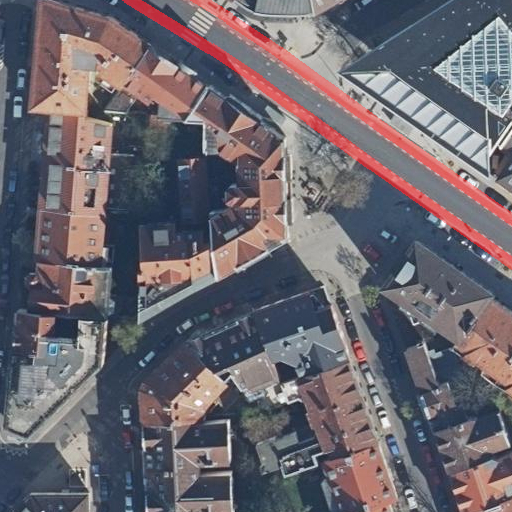
\includegraphics[width=0.35\textwidth]{Bilder/cut-example.jpg}
	\vspace{-10pt}
	% Das folgende ist ein Trick, um "Abbilgung x.y" in eine
	% eigene Zeile zu packen. Der Text zwischen [ und ] steht
	% im Abbildungsverzeichnis. Der Text darunter wird
	% tatsächlich angezeigt.
	\caption[Beispiel $512\times 512$-Ausschnitt aus Bike-Datensatz.]{\unskip}
	Beispiel $512\times 512$-Ausschnitt aus Bike-Datensatz mit roter Maske.
	\label{fig:cut-example}
\end{wrapfigure}

Jedes $10.000\times 10.000$-Pixel-Bild und die dazugehörige Maske wird -- um den gesamten Bildinhalt zu erhalten -- in \textit{auf}gerundet
$\left\lceil{\frac{10.000}{512}}\right\rceil^2 = 400$ Teile geschnitten. 
Die aufgerundeten 39 Ausschnitte, die nur partiell im Bild liegen, werden im überstehenden Bereich mit Schwarz ($RGB=(0,0,0)$) gefüllt.
Damit ergeben sich bei 143 Bildern $143 \cdot 400 = 57.200$ $512 \times 512$-Bildausschnitte. \\
Weiter werden alle Ausschnitte entfernt, die keine oder fast keine als Radweg annotierten Pixel beinhalten. 
Die Quote wird auf 1\% festgelegt. Sollte also ein Bildausschnitt weniger als 1\% Fahrradweg-Pixel beinhalten, 
wird es entfernt. Durch diese Maßnahme sinkt die Anzahl an Bildausschnitten von $57.200$ auf $10.181$ Bildausschnitte - 
dieser Anteil entspricht ca. 17,7\%. 
 
\autoref{fig:cut-example} zeigt beispielhaft ein auf $512\times 512$ Pixel zugeschnittenes Bild aus dem Bike-Datensatz 
mit der dazugehörigen Maske, die mit 50\% Transparenz in rot überlagert ist. Es ist zu erkennen, 
dass die Klassenimbalance noch recht stark ist, allerdings deutlich geringer, als in den ursprünglichen Bildern,
und dass auch trotzdem genügend Straßen ohne Radwege vorhanden sind und die Struktur und der Verlauf des Radweges 
bei der gewählten Ausschnittgröße weiterhin gut zu erkennen ist. 

\subsection{Training-Validation-Test-Split}

Zunächst werden die zerschnittenen Bilder aller Städte gemischt. Dann werden diese Ausschnitte disjunkt in 
Training-, Validation- und Test-Daten aufgeteilt. 
Damit sollten die unterschiedlichen Städte gleichermaßen in allen Teil-Datensätzen auftauchen, 
sodass der Test- und Validationdatensatz gut die Generalisierungsfähigkeit des Netzes überprüft. 
Durch die bereits höhere Zahl an Bildausschnitten (10.181 Stück) ist es eher unwahrscheinlich, 
dass eine ungleiche Verteilung der Städte vorkommt. Außerdem ist das Mischen wichtig, 
damit die Randausschnitte, die große schwarze Flächen beinhalten, anteilig gleich in 
jedem Teildatensatz repräsentiert sind, damit dies das Ergebnis nicht verfälscht, falls diese 
zum Beispiel nur in dem Validation- oder Testdatensatz vorkommen. 

\autoref{tab:bike-split} zeigt den im Folgenden verwendeten Trainings-Validation-Test-Split. 
Hierbei sind zwei Dinge zu bemerken, die nicht aus der Tabelle hervorgehen: 
Zunächst wurde der Testdatensatz abgespalten. Hierzu wurden 15\% vom Hannover-Datensatz und 
20\% von den jeweiligen Datensätzen der restlichen Städte als Testdatensatz abgespaltet. Da der Hannover-Datensatz so groß ist, wie die Datensätze der
restlichen Städte zusammen, läuft dies auf einen eher unkonventionellen Split von 17,5\% Testdaten hinaus. Diese Verteilung wurde so getroffen, 
um den Hannover-Datensatz etwas weniger zu gewichten, um im Test die Generalisierungsfähigkeit besser testen zu können
und den Einfluss der kleineren Städte auf die Generalisierungsfähigkeit zu erhöhen. Der Validation-Teildatensatz wurde danach aus 8\%, 
bzw. der Trainingsdatensatz aus 92\% vom Rest gebildet. \\
Der Trainingsdatensatz ist mit ca. 75\% der gesamten Daten eher groß gewählt, während der Validation-Datensatz eher klein gewählt ist. 
Nun kann ein größerer Validation-Datensatz dazu beitragen, die Hyperparameter besser zu optimieren. Das soll allerdings nicht Fokus der Arbeit sein.
Diese Entscheidung des großen Trainingsdatensatzes wurde getroffen,
um möglichst viele und unterschiedliche Bilder zum Training zu verwenden, da der Datensatz mit automatischer Synthese 
generiert wurde und daher qualitativ eher unvorteilhaft ist, wodurch eine höhere Anzahl an Trainingsdaten nötig wird.

\begin{table}
	\centering
	\begin{tabular}{l|l|l|l|l}
		& Training & Val. & Test & Summe \\
		\midrule
		Absolut & 7738 & 672 & 1771 & 10181 \\
		Anteil & 75,9 & 6,6 & 17,5 & 100 \\ 
	\end{tabular}
	\caption{Training-Validation-Test-Split des Bike-Datensatzes in gefilterten $512 \times 512$-Ausschnitten.}
	\label{tab:bike-split}
\end{table}


\subsection{Augmentation}

Die Bild-Augmentation wird nicht vor dem Training angewandt, um den Datensatz künstlich zu vergrößern, 
sondern während dem Training pseudo-zufällig mit festem Seed, um die Ergebnisse reproduzieren zu können.
Somit wird jedes Bild während des Trainings, bevor es in das Netz eingegeben wird zufällig augmentiert 
und dann eingegeben. Damit erhält ein und dasselbe Bild über die verschiedenen Epochen jedes Mal unterschiedliche 
Anpassungen auf Basis des Zufallsgenerators. Dies erhöht die Generalisierungsfähigkeit bzw. 
verringert die Gefahr von Overfitting. Das Netz sieht so viel mehr Varianten der Bilder. 
Nachteil ist, dass das Training länger dauert, da jedes Bild vor Eingabe bearbeitet wird. 
Dieser Nachteil ist vor allem evident, wenn mehrere Netze auf demselben Datensatz trainiert werden, da jedes Mal 
dieselben Augmentationen (da gleicher Seed) erneut vorgenommen werden müssen. Dieses Problem kann
durch eine Vorausberechnung der aufeinanderfolgenden Augmentationen behoben werden, worauf allerdings verzichtet wird. 

Jede der folgenden Augmentationen, wie beispielhaft zu sehen in \autoref{fig:augmentation}, wird in ihrem Wertebereich pseudo-zufällig angewandt. 
Sollte es die Veränderung erfordern, werden fehlende Bildteile mit Schwarz gefüllt. Schwarz wurde ausgewählt, da es ohnehin Bilder mit 
schwarzen Rändern im Datensatz gibt, weswegen das Netz hierbei mit nichts Neuem konfrontiert ist. 
\begin{enumerate}
	\item Rotation im Intervall von $[-90^\circ ; 90^\circ ]$. Eine Gradzahl wird für jedes Bild zufällig ausgewählt und angewandt. 
	Die dabei entstehenden leeren Bildbereiche werden mit Schwarz ($RGB = (0,0,0)$) gefüllt. 
	Diese Augmentation ist realistisch und nützlich, da Straßen in beliebiger Ausrichtung vorkommen und 
	eine natürliche Orientierung bei Bildern aus der Vogelperspektive nicht besteht.
	\item Horizontale Spiegelung. Es wird zufällig entschieden, ob ein Bild an der vertikalen Spiegelachse gespiegelt wird. 
	Diese Augmentation ist ebenfalls realistisch und hat gegenüber der Rotation den Vorteil keine schwarzen Flächen 
	einzuführen aber den Nachteil, nicht so viele neue Bilder erzeugen zu können. 
	\item Vertikale Spiegelung. Funktioniert wie die horizontale Spiegelung, allerdings wird an der horizontalen Achse gespiegelt. 
	Beide Spiegelungen können simultan auftreten, es gibt also vier Spiegelungs-Permutationen, 
	die mit gleicher Wahrscheinlichkeit auftreten.
	\item Horizontale Verschiebung im Intervall von $[-0,1 \cdot w; 0,1 \cdot w]$ Pixel entlang der horizontalen Achse,
	wobei $w$ die Breite des Bildes ist. Es wird eine zufällige Länge aus dem Intervall ausgewählt und verschoben; die 
	entstehenden Ränder werden mit Schwarz gefüllt. Auch diese Augmentation ist realistisch und erhöht lediglich 
	die Möglichkeit der Veränderung der Bilder. 
	\item Vertikale Verschiebung im Intervall von $[-0,1 \cdot h; 0,1 \cdot h]$ Pixel entlang der vertikalen Achse,
	wobei $h$ die Höhe des Bildes ist. Ansonsten ist die vertikale Verschiebung wie die horizontale Verschiebung.    
\end{enumerate} 

\autoref{fig:augmentation} zeigt eine beispielhafte Augmentierung des Bildes und der dazugehörigen Maske aus \autoref{fig:cut-example},
wobei eine horizontale Spiegelung\footnote{Die Spiegelachse ist hierbei \textit{vertikal}.},
eine Rotation um 13° und eine Verschiebung um 8\%, also $\lceil 0,08 \cdot 512 \rceil = 41$ Pixel, 
nach links dargestellt ist. Es ist keine vertikale Spieglung oder vertikale Verschiebung vorhanden.
Die Randbereiche, wofür aufgrund der Verschiebung und Rotation keine Daten vorhanden sind, sind mit Schwarz gefüllt. 

Die angewandten Augmentationen sind eher konservativ gewählt. An den Bildern wird kaum etwas verändert, 
außer die Pixel leicht umzusetzen. Dadurch würde ein augmentiertes Bild im Original-Datensatz nicht auffallen. 
Auf weitergehende Veränderungen wie Gamma-Korrektur, Helligkeitsanpassung, Zoom und Scherung wird hingegen verzichtet. 
Diese Veränderungen werden nicht vorgenommen, um mit dem Testdatensatz besser abschätzen zu können, 
wie gut die Erkennung der Radwege allgemein - unter optimalen Bedingungen - funktioniert, ohne zunächst auf 
maximale Generalsierungsfähigkeit zu untersuchen. Diese Abschätzung wird dann mithilfe des Testdatensatzes von 
Karlsruhe, welcher im Erscheinungsbild stark vom Bike-Testdatensatz abweicht, vorgenommen, 
indem die Ergebnisse für den Bike-Testdatensatz und den Karlsruhe-Datensatz verglichen werden. 

\begin{figure}
	\centering
	\begin{minipage}{.45\textwidth}
		\centering
		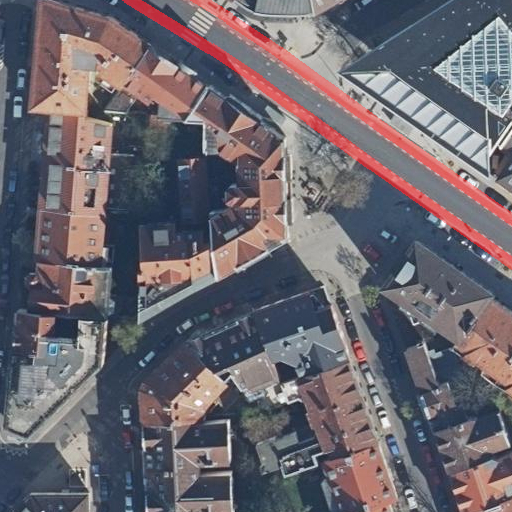
\includegraphics[width=.7\linewidth]{Bilder/cut-example.jpg} 
	\end{minipage}
	\begin{minipage}{.45\textwidth}
		\centering
		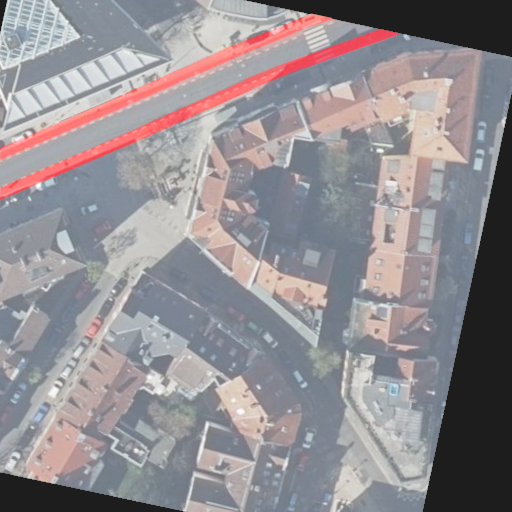
\includegraphics[width=.7\linewidth]{Bilder/augmentation-example.png} 
	\end{minipage}

	\caption{Beispielhafte Datenaugmentation mit Originalbild und Maske in Rot links 
	und augmentiertes (horizontale Spiegelung, Rotation, Verschiebung nach links) Bild 
	mit Maske in Rot rechts.  }
	\label{fig:augmentation}
\end{figure} 

% augmentation = {
% 	"rotation_range": 90,
% 	"width_shift_range": 0.1,
% 	"height_shift_range": 0.1,
% 	"fill_mode": "constant",
% 	"cval": 0,
% 	"horizontal_flip": "True",
% 	"vertical_flip": "True",
% 	"validation_split": 0.08

\section{Evaluationsmaße}

Dieses Kapitel bezieht alle Evaluationsmaße auf eine semantische Segmentierung, wobei jedem Pixel genau ein Output-Neuron 
zugeordnet ist und der Pixel als Fahrradweg bei Aktivierung bzw. als Hintergrundpixel bei fehlender Aktivierung klassifiziert wird --
es handelt sich also nicht um eine One-Hot-Kodierung.

Als eine direkte und intuitiv sehr anschauliche Metrik zum Bewerten der Modellperformanz bei Segmentierungsproblemen
kann \ac{IoU} herangezogen werden. \\ 
Problematisch an der \ac{IoU} ist, dass alle möglichen Klassifikationen ($tp$, $fp$, $fn$, $tn$)
gleich stark gewichtet werden, wobei die wahr-positiven $tp$ zunächst Priorität haben sollten, 
während die Fehler der falsch-positiven $fp$ und falsch-negativen $fn$ im Gleichgewicht bleiben sollten, 
sodass es nicht zu einer trivialen Klassifikation als rein positiv oder rein negativ kommt. \\
Ein weiteres Problem ist, dass die \ac{IoU} sehr streng und intolerant gegenüber leichter Verschiebung der Erkennung 
bewertet. Wenn ein Fahrradweg, der nur wenige Pixel breit ist, um die Hälfte der Breite verschoben segmentiert würde
aber ansonsten komplett dem Radweg entspricht, würde die \ac{IoU} bereits von 1 auf 0,5 sinken, obwohl \textit{qualitativ} 
der Weg exakt erkannt wurde. Diese Intoleranz gegenüber leichter lokaler Verschiebung ist insbesondere in dem 
in dieser Arbeit vorgestellten Bike-Datensatz aus \autoref{sec:bike-data} problematisch, 
da dieser über \ac{OSM} annotiert ist und für viele Straßen die Lage des zugehörigen Radwegs heuristisch über 
die Spuranzahl ermittelt wird. \\
Aufgrund der genannten Einschränkungen ist die \ac{IoU} ungeeignet als Verlustfunktion, kann jedoch als ein Maß 
in die Bewertung der Modellperformanz mit einfließen. 

Dice: löst ungleichgewichtsproblem aber keine toleranz zu verschiebung der radwege. 
Optimal für Hand-annotierter Datensatz

BCE klassenimbalance problem und weniger backing in roads stuff

kombinierte Maße (BCE + Dice ? ) manchmal gut wie research zeigt

\subsection{\acf{BIoU}} \label{sec:eval:biou}

Für den Spezialfall von semantischer Segmentierung zur Erkennung von Radwegen muss für die \textit{Quality} (vgl. \autoref{sec:evaluation-metrics:quality}) 
eine Berechnungsmöglichkeit ermittelt werden, um die Quality auf diskreten Rastern, also den Bildern und Masken, anwenden zu können.
Hierfür wird der Name der \textit{\acf{BIoU}} eingeführt, der fortan für die Quality mit Anwendung auf semantische Segmentierung verwendet wird.

Sei $P$ die Prediction der Segmentierungsmaske für ein Eingabebild, $Y$ die tatsächliche Segmentierungsmaske (Ground-Truth / Label)
und $P, Y \in \{0, 1\}^{w \times h}$, wobei $w$ und $h$ die Breite und Höhe des Eingabebildes darstellen.
Die Einträge mit Wert eins von $P$ und $Y$ sind Radweg, die Einträge mit Wert null Hintergrund. Einträge repräsentieren Pixel.
$B$ sei die Puffergröße in Pixeln. \\
Zunächst sei die Hilfsfunktion $dilate_B: \{0,1\}^{w \times h} \mapsto \{0,1\}^{w \times h}$ definiert als 
\newcommand{\norm}[1]{\left\lVert#1\right\rVert}
\begin{align}
	\label{eq:dilate} dilate_B(A) = \left( \begin{cases} 
		1 & \exists a_{kl} \in A: a_{kl} = 1 \land \norm{
			\begin{pmatrix} k \\ l \end{pmatrix} - \begin{pmatrix} i \\ j \end{pmatrix} }_2 \leq B \\
		0 & else 
	\end{cases} \right)_{ij}~.
\end{align}
Die Funktion $dilate_B$ bildet eine Matrix auf eine weitere derselben Ordnung ab, 
sodass alle Einträge gleich eins sind, die in der Eingabematrix eins sind. Zusätzlich sind alle Einträge eins, 
die im Umkreis von $B$ Pixel um eine Eins in der Eingabematrix liegen. Somit werden die positiven (Wert = 1)
Pixel der Eingabematrix um die Bufferzone erweitert.  \\
Damit lassen sich die gepufferten, fehlertoleranteren wahr-positiv $tp_B$, falsch-positiv $fp_B$ und 
falsch-negativ $fn_B$ Werte berechnen: 
\begin{align}
	\label{eq:buffering} {tp}_B = \norm{dilate_{B}(Y) \odot P}_{1,1} , \\
	fn_B = \norm{Y - (Y \odot dilate_{B}(P))}_{1,1} , \\
	{fp}_B = \norm{P}_{1,1} - {tp}_B .
\end{align}
Beispielhaft und intuitiv dargestellt für $tp_B$: Es sollen auch alle Eins-Pixel als wahr-positiv aufgefasst werden,
die leicht von der Ground-Truth abweichen, also sich noch in der Pufferzone befinden. 
Hierfür wird die Pufferzone um die Ground-Truth $Y$ gelegt und das Hadamard-Produkt mit der Predicition $P$ gebildet.
Da alle Matritzen als Einträge nur 0 oder 1 enthalten, findet durch das Hadamard-Produkt eine Art Verundung statt, 
sodass im Produkt nur Einträge eins sind, die in beiden Matritzen eins sind. Der Rest ist null. 
Durch die zuvor durchgeführte Pufferung mit $dilate_B$ sind allerdings auch Einträge gleich eins, die in $Y$ 
zuvor null waren. Hierdurch besitzt das Hadamard-Produkt mehr Einträge mit eins, als bei der Berechnung der \ac{IoU}.
Diese Zahl ist genau um die Anzahl an positiven Pixeln aus $P$ größer, die in der Pufferzone liegen. 
Schließlich wird mit der $1,1$-Höldernorm für Matritzen die Anzahl an Einsen gezählt, was dann $tp_B$ ergibt. \\
Die Formel für die \ac{BIoU} ist analog zur \ac{IoU}, bis auf die Verwendung der jeweils gepufferten 
Variablen:\footnote{\autoref{code:quality} zeigt die dazugehörige Python-Implementation.}
\begin{align}
	\label{eq:quality} BIoU = \frac{tp_B}{tp_B + fp_B + fn_B} ~.
\end{align}

Die \ac{BIoU} adressiert das Verschiebungs-Problem der \ac{IoU} mit einem Puffer zur relaxierteren Ermittlung der 
$tp$, $fp$ und $fn$. Hierbei ist allerdings die Puffergröße in Pixeln eine wichtige Stellschraube.  
Da ein Radweg im Mittel ca. 11,8 Pixel und eine Straßenfahrbahn ca. 17,6 Pixel breit ist (s. \autoref{sec:bike-data}), 
wird der Buffer als ganze Zahl auf das arithmetische Mittel $\frac{11,8 + 17,6}{2} = 14,7 \approx 15$ festgelegt. 
Dies erlaubt eine Verschiebung des Radwegs um eine volle Breite zzgl. einer Toleranz für die leicht variierende Radwegbreite, 
nicht aber um die Breite einer Straßenfahrbahn. Hiermit soll ein realistisches Bild der Performanz des Netzes 
bezgülich der qualitativen Erkennung der Radwege gezeichnet werden und wird ergänzend zur \ac{IoU}-Metrik 
als Bewertungsfunktion eingesetzt. \\
Als Verlustfunktion ist die \ac{BIoU} allerdings ungeeignet, da wie bei der \ac{IoU} die wahr-positiven $tp$ nicht 
stärker gewichtet werden, sodass das Netz nicht bevorzugt die wahr-positiven lernt. Des Weiteren ist die \ac{BIoU} aufgrund der 
in \autoref{eq:dilate} beschriebenen Dilate-Funktion nicht bekannt differenzierbar, was für die Verlustfunktion nötig ist. 
Gegebenenfalls kann eine Ableitung für die \ac{BIoU} gefunden werden, 
die Untersuchung dessen geht allerdings über den Umfang dieser Arbeit hinaus. 
Zuletzt wird das Verwenden der \ac{BIoU} als Loss-Funktion - unter der Prämisse, dass dies möglich ist - einen weiteren 
Hyperparameter - die Puffergröße - einführen, was weiter die Komplexität des Modells erhöht.  

\section{Architektur} \label{sec:architecture}

Im Folgenden werden die untersuchten Architekturen genauer beschrieben und ebenfalls begründet, 
warum die jeweiligen architektonischen Entscheidungen getroffen wurden. \\
In \autoref{sec:state-of-the-art-roads} wurde ausführlich der Stand der Technik und Wissenschaft 
im Bereich der Straßenerkennung und -extraktion mittels Computer-Vision-Modellen beschrieben. 
Aufgrund der Ähnlichkeit der Problemdomäne lässt sich vermuten, dass ähnliche Verfahren wie 
zum Erkennen von Straßen auch für das Erkennen von Fahrradwegen nützlich sein können. 
Die Problemdomänen sind ähnlich, da Fahrradwege auch Straßen sind und eben jene Eigenschaften, 
wie große Klassenimbalance zwischen Fahrradweg und Hintergrund, Beschattung durch andere Objekte,
Verdeckung durch z.B. Bäume und ähnliche Annotationsfehler   
teilen. Schwierigkeit ist, Fahrradwege von Straßen zu unterscheiden. \\
Die Radwege sollen, wie Straßen auch, mittels Image-Semantic-Segmentation von einem Computer-Vision-Modell 
markiert werden. Andere Klassifizierungsarten, wie die in \autoref{sec:aufgabenkategorien} beschriebene 
Objektdetektion würde zu grobe Bounding-Boxes um schräg verlaufende Radwege legen, sodass im Prinzip 
eine Straße markiert werden würde, die zwar einen Radweg hat, aber nicht klar wäre, wo dieser verläuft, 
bzw. ob ein Radweg in beide Richtungen existiert. Aus demselben Grund ergibt eine reine Klassifikation, 
ob ein Bild einen Radweg enthält oder nicht ebenfalls keinen Sinn. 
Auf der anderen Seite würde Instanz-Segmentierung keine weiteren relevanten Informationen hinzufügen, 
wonach semantische Segmentierung ausreicht, um das Problem zu lösen. \\
Wie bereits in \autoref{sec:state-of-the-art-roads} dargelegt sind alle relevanten Modelle zur 
Straßenerkennung basierend auf der U-Net-Archtiektur (vgl. \ref{sec:architekturkomponenten:unet}).
Folglich sollen die hier betrachteten Modelle ebenfalls als angepasste U-Nets entworfen werden. 
Insbesondere ermöglicht dies auch die Modelle zur Fahrradwegerkennung auf den verschiedenen 
in \autoref{sec:road-detection:roads-data} vorgestellten Datensätzen zur Straßenerkennung vorzutrainieren, 
was zu allgemein besseren Ergebnissen führen kann (s. \autoref{sec:transfer-learning}). 
Außerdem können so die erzielten Ergebnisse vom Pre-Training mit den öffentlichen Benchmarks verglichen werden,
um deren Ergebnisse zu validieren und früh Fehler in den eigenen Entscheidungen und Implementationen zu entdecken.

\renewcommand{\labelenumii}{\theenumii}
\renewcommand{\theenumii}{\theenumi.\arabic{enumii}.}

Zunächst soll so ein nur leicht modifiziertes U-Net, welches im Folgenden \textit{\acf{BUNet}} 
genannt wird, entworfen werden, welches als Baseline- und Vergleichs-Netz dienen soll und 
wovon es zwei Komplexitätsvarianten, das \ac{BUNet2} mit 2 Mio. Parametern und das \ac{BUNet15} 
mit 15 Mio. Parametern geben soll. \\
Dann soll eine zweite Klasse an U-Nets beschrieben werden, die verschiedene vortrainierte \acp{CNN} (s. \autoref{sec:pretrained-backbones}) 
als Backbones für ein U-Net verwendet, da \autoref{sec:state-of-the-art-roads} gezeigt hat, 
dass im Falle der Straßendetektion die Performanz eines Netzes stark verbessert werden kann, 
indem auf Techniken und Methoden von Modellen aus anderen Teilgebieten der Computer-Vision 
zurückgegriffen wird. 
Gegebenenfalls ist das auch für die Radwegerkennung möglich. Dazu sollen mehrere Backbones untersucht werden, 
da die gewählten Backbones jeweils gut für die Straßenerkennung funktioniert haben und sich 
herausstellen soll, ob es einen besonders guten Backbone für die Radwegerkennung gibt. 
Folgende Liste zeigt eine Übersicht über die Netze, während die nachfolgenden Abschnitte genauer 
den erläutern und begründen, warum ein Backbone gewählt wurde: 
\begin{enumerate}
	\item \textit{\acf{BUNet}}: Baseline Netz ohne Backbone.
	\begin{enumerate}
		\item \textit{\acf{BUNet2}}: Variante mit 2 Mio. Parameter.
		\item \textit{\acf{BUNet15}}: Variante mit 15 Mio. Parameter.
	\end{enumerate}
	\item Backbone-U-Nets
	\begin{enumerate}
		\item \textit{\acf{VBUNet}}: Baseline Netz mit Baseline-Backbone.
		\item \textit{\acf{RBUNet}}: Hoch-performant bei Straßenerkennung.
		\item \textit{\acf{DBUNet}}: Hoch-performant bei Straßenerkennung.
	\end{enumerate}
\end{enumerate} 

\subsection{Bike-U-Net} \label{sec:architecture:bike-u-net}

\autoref{fig:bike-unet-2} zeigt die verwendete Architektur für das \textit{\ac{BUNet2}}. 
Hierfür wurde das in \autoref{fig:u-net-architecture} 
dargestellte originale U-Net auf den vorliegenden Anwendungsfall angepasst.
Diese Anpassungen sind in der nachfolgenden Liste erklärt.

\begin{itemize}
	\item Zunächst werden Input-Bilder der Größe $width \times height \times 3$ verwendet. 
	Wobei $width$ und $height$ variabel in der Architektur sind, mit der Einschränkung, 
	dass diese Vielfache von 32 sein sollten, damit die mittlere Schicht nicht zu klein wird. 
	In jedem Fall wird ein Bild mit drei Kanälen (RGB) verwendet. 
	In der Abbildung ist exemplarisch $512 \times 512 \times 3$ gewählt. \\
	Der Output verwendet zunächst keine explizite One-Hot-Kodierung für Fahrradweg und Hintergrund, 
	sondern eine mit lediglich einem Output-Neuron, wobei keine Aktivierung einen Hintergrundpixel 
	und eine Aktivieriung ein Radweg-Pixel impliziert, wie in \autoref{sec:state-of-the-art-roads} beschrieben, 
	um eine intuitivere Bewertung zu ermöglichen. 
	\item Im Gegensatz zum originalen U-Net, wird bei den Convolutional-Layern Padding eingesetzt,
	um die Dimensionen der Feature-Maps nicht nach und nach zu verkleinern und so einen exakt symmetrischen Aufbau zu gewährleisten.
	Ebenso wurde bei den Up-Convolutions Padding eingefügt, um auch hier eine Verkleinerung der Feature-Maps zu verhindern.
	Diese Anpassung wurde eingesetzt, um kein Zuschneiden bei den Skip-Connections zu benötigen, was die Lokalisierung verbessern soll,
	und so bei den in \autoref{sec:state-of-the-art-roads} beschriebenen Netzen gewöhnlich ist.
	\item Im originalen U-Net beginnt der erste Convolutional-Block mit 64 Filtern, 
	welche sich jeden weiteren Block mit zum Mittel-Block verdoppeln, der dann 1024 Filter besitzt.
	Daraufhin halbieren sich die Filter mit jedem weiteren Decoder-Block wieder. \\
	Im Bike-U-Net-2 beginnen die Filter bei 16 und verdoppeln sich bis 256, was zu ungefähr 2 Mio. 
	trainierbaren Parametern führt. Die Zahl an Parametern ist somit weitaus geringer als im 
	Original-U-Net mit ca. 24 Mio. Parameter \cite{Ronneberger.18052015}. 
	Hiermit soll getestet werden, ob auch ein recheneffzienteres und kleineres U-Net gute Ergebnisse liefert, 
	und somit auch weniger Regularisierung notwendig ist. \\
	Da aber die in \autoref{sec:state-of-the-art-roads} beschriebenen Netze ebenfalls 15-25 Mio. Parameter haben, 
	soll ein weiteres U-Net mit mehr Parametern getestet werden. Das \textit{\ac{BUNet15}} hat 15 Mio. 
	Parameter\footnote{\autoref{fig:bike-unet-15} zeigt \ac{BUNet15}}. Dies wird erzielt, 
	indem die Filteranzahl ab dem zweiten Block dreimal höher ist als in \ac{BUNet2}. So sind hier 16 Filter in Block eins, 
	dann 96 Filter in Block zwei, die sich verdoppeln bis hin zu 768 Filtern im mittleren Block und danach wieder halbieren bis zum vorletzten Block. 
	Dabei hat der letzte Block wieder 16 Filter. 
	Der erste und letzte Block haben jeweils 16 Filter, da damit der Rechen- und Speicheraufwand erheblich reduziert werden kann.
	Bis auf die Filteranzahl und die daraus resultierende Tiefe der Feature-Maps, sind \ac{BUNet2} und Bike-U-Net-15 identisch.
	\item Auf jede Convolution-Schicht folgt eine Batch-Normalization-Schicht. 
	Dies hat mehrere Gründe: Zum einen übernimmt so das Netz selbst die Normalisierung und Standardisierung der Daten, 
	wodurch sich das beim Vorverarbeiten gespart werden kann und zum anderen kann von den in \autoref{sec:architekturkomponenten:batchnorm} 
	beschriebenen Vorteilen, wie schnellerem Training profitiert werden, 
	ohne, dass dafür zusätzlicher Aufwand betrieben werden muss und keine Nachteile entstehen.
	\item Zusätzlich zu den Batch-Normalization-Schichten werden pro Block eine Dropout-Schicht 
	nach der jeweils ersten Convolution-Schicht eingezogen. Diese sollen als 
    Hyperparameter eingebaut werden, um einfach kontrollierbar Regularisierung anzuwenden, 
	falls die Modelle Probleme mit Overfitting durch zu hohe Komplexität bekommen. 
	Aufgrund der eher wenigen Parameter wird dies aber gegebenenfalls nur beim \ac{BUNet15}, 
	oder überhaupt nicht nötig.
	\item Die Convolution-Schichten werden durch \ac{ELU} (s. \autoref{sec:activation:elu}) aktiviert, 
	anstatt durch \ac{ReLU}, wie im Original-U-Net. 
	Hierdurch können die meisten der in \autoref{sec:activation} herausgearbeiteten Vorteile von \ac{ReLU},
	wie Robustheit gegen das Vanishing-Gradient-Problem, genutzt werden. Jedoch wurde bereits im ursprünglichen U-Net-Paper 
	(\cite{Ronneberger.18052015}) beschrieben, dass Netzteile under \ac{ReLU} dauerhaft inaktiv werden (Dying-Neuron-Problem). 
	Deshalb wurde hier auf \ac{ELU} zurückgegriffen, da damit alle Netzteile aktiv bleiben sollen. 
	Nachteil ist hierbei, dass die Berechnung von \ac{ELU} etwas aufwendiger ist. 
	Das Problem von unbeschränkt großen positiven Aktivierungen unter denen sowohl \ac{ELU} als auch \ac{ReLU} leiden,
	wird in diesem Netz durch die wiederholte Batch-Normalisierung abgefedert.
	\item Für das Ouptut-Layer, nach der $1\times 1$-Convolution, wird die Sigmoid-Funktion verwendet. 
	Im Falle einer One-Hot-Kodierung würde hier Softmax herangezogen werden. 
\end{itemize}

\begin{figure}
	\centering
	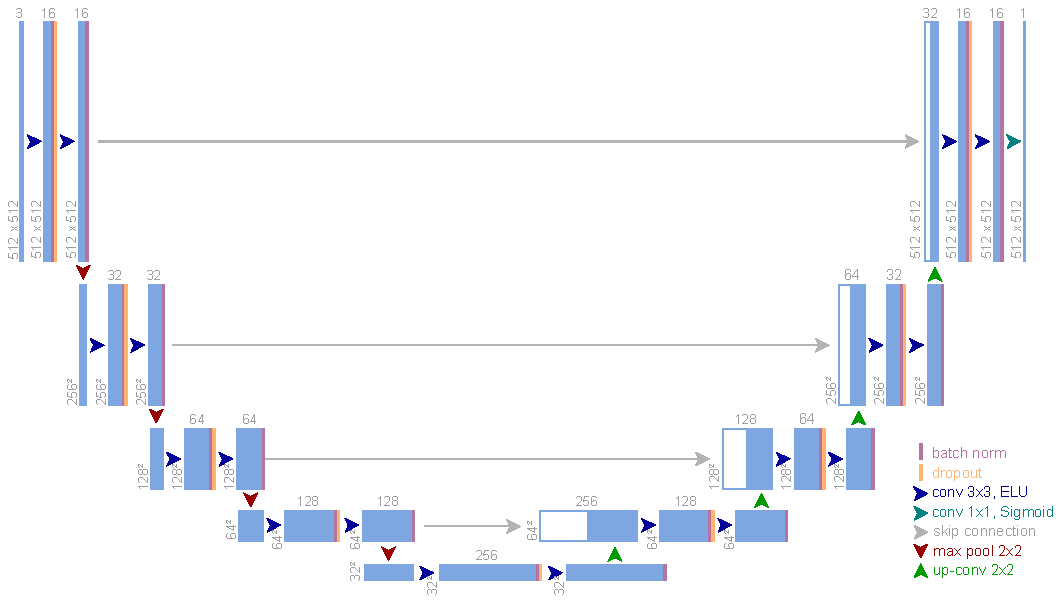
\includegraphics[width=1.\textwidth]{Bilder/own-unet-2mil.pdf} 
	\caption{Bike-U-Net-2 mit 1,946 Mio. Parametern.}
	\label{fig:bike-unet-2}
\end{figure} 

% HE INITIALIZATION

\subsection{Backbone-U-Nets}

Prinzipiell dienen die Convolution-Schichten aller in \autoref{sec:pretrained-backbones} beschriebenen vortrainierten Backbone-Netze 
der Feature-Erkennung und -Extraktion. Lediglich die letzten Schichten, die bei den beschriebenen Klassifikationsmodellen  
Fully-Connected-Schichten waren, sind für die Zuordnung der Features zu den Objektklassen 
im ImageNet-Datensatz notwendig. Werden diese Schichten mit einem Decoder-Teil, der den Encoder - hier 
also das vortrainierte Klassifikationsnetz - spiegelt, ersetzt, entsteht ein Modell zur semantischen Segmentierung. 
Weiter müssen lediglich an geeigneter Stelle Skip-Connections zwischen Encoder und Decoder eingefügt werden,
um die U-Net-Form nachzubilden. Im Folgenden werden die auf diese Weise konstruierten Netze beschrieben. 

\subsubsection{VGG16-Bike-U-Net}

\textit{\ac{VBUNet}} nutzt das in \autoref{sec:pretrained-backbones:vgg16} beschriebene Netz VGG16 
mit auf ImageNet vortrainierten Gewichten als Backbone. \\
Hierzu werden die drei Fully-Connected-Layer 
(und Soft-Max-Aktivierung) am Ende entfernt und mit drei neuen \textit{conv3-512}-Schichten ersetzt. 
Diese bilden den mittleren (\enquote{untersten}) Block im U-Net. Darauf folgt eine direkte Spieglung 
von VGG16 als Decoder mit abschließender $1\times 1$-Convolution. Im Gegensatz zum Bike-U-Net (s. \autoref{sec:architecture:bike-u-net}) 
und ursprünglichen U-Net (s. \autoref{sec:architekturkomponenten:unet}) wurden allerdings keine 
\textit{up-conv3}-Layer mit trainierbaren Gewichten zum Upsampling genutzt, sondern 2D-Upsampling-Layer, 
ohne trainierbaren Parameter. Diese Entscheidung wurde getroffen, um VGG16 besser nachzuempfinden, 
da hier Maxpool-Schichten zum Downsampling verwendet werden, die ebenfalls keine trainierbaren Parameter enthalten.
Weiter sind nach jeder nicht-vortrainierten Convolution-Schicht, also nach jeder, die nicht zu VGG16 gehören, 
Batch-Normalization-Layer eingezogen, aus den in \autoref{sec:architecture:bike-u-net} und \autoref{sec:architekturkomponenten:batchnorm}
genannten Gründen wie schnellerem Training, leichter Glättung und fehlender sonstiger Standardisierung und Normalisierung.
Die für U-Net charakteristischen Skip-Connections werden vor jeder Maxpool-Schicht außer der ersten eingesetzt 
und mit dem korrespondierenden Decoder-Block verbunden. Dies resultiert in genau vier Skip-Connections, 
wie im Bike-U-Net und originellen U-Net. Abgeschlossen wird durch eine Sigmoid-Aktivierung, so wie im Bike-U-Net. \\
VGG16-Bike-U-Net enthält 23,7 Mio. Parameter. Grob die Hälfte davon (14,7 Mio.) sind von VGG16. 

VGG16 wird als Backbone ausgewählt und getestet, da es als eine Art Basis- bzw. Standardversion der nachfolgenden 
Backbone-Netze aufgefasst werden kann, da diese auf VGG16 aufbauen und dieses - zumindest 
für den ImageNet-Datensatz - verbessern und nachvollzogen werden soll, ob diese Anpassungen dienlich sind 
für den konkreten Anwendungsfall der Radwegerkennung. Zudem ist VGG16 sehr beliebt als vortrainiertes 
Netz, weswegen es viele Vergleichsmöglichkeiten gibt. 
Des Weiteren wird VGG16 als Backbone in Research zum Pre-Training mit U-Nets eingesetzt (s. \autoref{sec:transfer-learning:backbones}), 
auf dessen Ergebnisse diese Arbeit aufbaut. 
Demnach ist es wiederum für Vergleichszwecke sinnvoll VGG16 als Backbone für die Radwegerkennung zu verwenden.   

\subsubsection{ResNet34-Bike-U-Net}

\textit{\ac{RBUNet}} nutzt das in \autoref{sec:pretrained-backbones:resnet} beschriebene Netz ResNet34 
mit auf ImageNet vortrainierten Gewichten als Backbone. \\
Hierzu wird die eine Fully-Connected-Layer am Schluss des Netzes entfernt und um einen Decoder ersetzt. 
Anders als bei \ac{VBUNet} ist der mittlere Block der U-Net-Struktur von ResNet34 
und nicht zusätzlich neu ergänzt. Grund dafür ist die höhere Anzahl an Parametern 
von ResNet34, welche ohne die Fully-Connected-Schicht bereits bei 24,4 Mio. liegt, im Gegensatz zu VGG16. 
Da der mittlere Block die meisten Parameter beinhaltet, wird keine weitere Vertiefung des Netzes vorgenommen,
um die Anzahl der Parameter nicht drastisch zu erhöhen. An Stelle dessen wird nach Ende der Convolution-Schichten von 
ResNet34 direkt mit dem Upsampling begonnen, welches wie bei \ac{VBUNet} mit Upsampling-Schichten 
bewerkstelligt wird. Auch wird im Widerspruch zu \ac{VBUNet} der Encoder - also ResNet34 - nicht gespiegelt, 
um eine Verdoppelung der Parameteranzahl zu vermeiden. Stattdessen wird ein einfacher, U-Net-ähnlicher Decoder
aus fünf Blöcken á Upsampling-Schicht und zwei Convolution-Schichten verwendet, wobei in jedem Block 
die Filter-Anzahl von 512 an bis schließlich 16 halbiert wird. Abgeschlossen wird wie bei \ac{VBUNet} und
\ac{BUNet} mit $1\times 1$-Convolution und Sigmoid-Aktivierung. Aus den gleichen Gründen wie bei \ac{VBUNet}
sind nach jeder Convolution-Schicht Batch-Normalization-Schichten eingezogen. 
Es erfolgt wiederum das Einsetzen von vier Skip-Connection nach U-Net-Vorbild ergänzend zu den 
Skip-Connections der Residuen-Blöcke an folgenden Stellen: 
nach der $7\times 7$-Convolution zu Beginn von ResNet34, 
am Ende der Blöcke mit 64 Filter, am Ende der Blöcke mit 128 Filtern 
und am Ende der Blöcke mit 256 Filtern. Im Decoder werden diese jeweils 
zu Beginn der ersten vier Decoder-Blöcke konkateniert. \\ 
ResNet34-Bike-U-Net enthält 24,4 Mio. Parameter. Davon sind 21,2 Mio. von ResNet34 und lediglich 3,2 Mio. 
vom Decoder, welcher somit eher unterrepräsentiert ist im Netz.  

ResNet34 wird als Backbone ausgewählt und getestet, aufgrund der hohen Präsenz von 
Residual-Blöcken in den leistungsstärksten Modellen 
zur Straßenerkennung aus \autoref{sec:state-of-the-art-roads} und insbesondere \autoref{tab:optimized-benchmarks}.
Es wird sich ebenfalls eine bessere Performanz dieses Modells bei der Radwegerkennung erhofft. 

\subsubsection{DenseNet121-Bike-U-Net}

\textit{\ac{DBUNet}} nutzt das in \autoref{sec:pretrained-backbones:densenet121} beschriebene Netz DenseNet121 
mit auf ImageNet vortrainierten Gewichten als Backbone. \\
Hierzu wird der Classification-Layer bestehend aus einer $7\times 7$-Average-Pool-Schicht 
und einer Fully-Connected-Layer entfernt und durch einen Decoder ersetzt. 
Wie schon bei \ac{RBUNet} erstreckt sich das DenseNet bis in den mittleren U-Net-Block. Beim \ac{DBUNet} 
liegt der Grund dafür allerdings nicht in der hohen Parameterzahl, sondern in der hohen sonstigen Komplexität 
des Netzes. So benötigt DenseNet121 trotz deutlich geringerer Parameterzahl für die Inferenz und das Training länger 
als sowohl \ac{RBUNet}, als auch \ac{VBUNet}. Vermutlich ist hierfür die große Tiefe von 64 Schichten, wovon 
60 Convolution-Schichten sind, verantwortlich. Um die Inferenz- und Trainingszeit nicht weiter zu belasten, 
ist der Decoder eher simpel gehalten, enthält also wenig Parameter. Für den Decoder wird die gleiche Architektur wie im \ac{RBUNet} verwendet.
Auch hier sind die Batch-Normalization-Schichten eingezogen. Der Unterschied besteht darin, 
dass die erste Convolution-Schicht anders als bei \ac{RBUNet} nicht von 512 Kanälen auf 256 abbildet, 
sondern von 1536 auf 256. Dies liegt an der Konkatenierung der DenseNet-Architektur. Wieder wird das 
Netz abgeschlossen durch eine $1\times 1$-Convolution gefolgt von einer Sigmoid-Aktivierung. 
Auch hier werden wieder vier Skip-Connections eingebaut, um die U-Net-Architektur nachzuahmen. 
Diese Skip-Connections sind im Falle von \ac{DBUNet} im Encoderteil nach der ersten $7 \times 7$-Convolution 
und dann jeweils nach jeder weiteren $1\times 1$-Convolution der DenseNet-Transition-Zonen eingesetzt. 
Im Decoder-Teil sind diese wie bei \ac{RBUNet} zu Beginn jedes Decoder-Blocks bis auf den letzten eingebaut. \\
DenseNet121-Bike-U-Net enthält 12,1 Mio. Parameter, wovon 6,9 Mio. zum DenseNet121 und 5,1 Mio. neu hinzugefügt 
wurden. Trotz doppelter bzw. sogar vierfacher Tiefe besteht \ac{DBUNet} nur aus ungefähr halb so vielen 
Parametern wie \ac{RBUNet} und \ac{VBUNet}. 

DenseNet121 wird als Backbone ausgewählt, wegen der guten Ergebnisse von Dense-U-Net-121 aus \autoref{sec:state-of-the-art-roads}. 
Darüber hinaus werden zusammen mit VGG16 und ResNet34 Netze mit verhältnismäßig flacher, mitteltiefer und tiefer 
Architektur getestet, was eine Vielfalt an Architekturen abbildet.

\section{Hyperparameter}

\subsubsection{Batch-Size:}

Der Vorteil einer kleineren Batch-Size ist, dass das Netz besser lernt die Feinheiten der Daten abzubilden. 
Der Vorteil einer görßeren Batch-Size ist, dass das Netz schneller trainiert. 
Da allerdings Batch-Norm (vgl. \autoref{sec:architecture}) angewandt wird, würde eine Batch-Size von 1 (wie im originellen U-Net) keinen 
Sinn ergeben, da die Daten im Pre-Processing nicht normalisiert werden (vgl. \autoref{sec:pre-processing}), wodurch Batch-Norm alle 
Normalisierung übernimmt. Wenn das allerdings auf nur ein Bild angewandt wird, ist keine gute Normalisierung über den ganzen Datensatz zu erwarten. 
Eine große Batch-Size, wie z.B. 16, ist allerdings sehr ressourcenintensiv, da alle Elemente des Batches simultan in den Speicher geladen und verarbeitet 
werden müssen. \\
Als Kompromiss wird eine Batch Size von 4 festgehalten. Durch die zufälligen Batches ist eine angemessene Normalisierung zu erwarten.

\subsubsection{Dropout-Rate:}

Dropout soll dem Overfitting, was aufgrund der wenigen Trainingsdaten auftreten kann, entgegen wirken. 
Die Rate, mit der die Dropout-Layer Neuronen auf null setzen, wird nicht als ein konstanter Wert für das ganze Netz festgelegt, 
sondern nimmt im Encoder-Teil sukzessive zu und ab dem Decoder-Teil gespiegelt sukzessive ab, siehe \autoref{tab:dropout}. 
Das soll eine hohe Dropout-Rate im Mittelteil des Netzes ermöglichen, während die Rate in den äußeren Schichten eher niedrig ist. 
Dies ist erwünscht, damit in den äußeren Schichten, möglichst alle Inputs eingefangen werden bzw. die Outputs richtig lokalisiert werden. 
In den äußeren Schichten mit eher weniger Filtern und damit weniger Parametern stellt Overfitting ein geringeres Problem dar. 
Für die mittleren Layer mit ausgeprägten Feature-Maps, vielen Filtern und Parametern jedoch ein größeres Problem, weswegen hier ein eher größerer
Dropout erwünscht ist.     

\begin{table}[ht]
	\centering
	\begin{tabular}{r|ll|ll|l|ll|ll}
		\textbf{Block} & 1 & 2 & 3 & 4 & 5  & 6 & 7 & 8 & 9 \\
		\midrule
		\textbf{Rate} & 0,1 & 0,1 & 0,2 & 0,2 & 0,3 & 0,2 & 0,2 & 0,1 & 0,1 \\ 
	\end{tabular}
	\caption{Dropout-Raten der unterschiedlichen Blöcke in \ac{BUNet}.}
	\label{tab:dropout}
\end{table}

\subsubsection{Learning-Rate:}

Als Learning-Rate wird ein Faktor von $0,0001$ angesetzt. Dieser Wert wird in einigen verwandten Problemen mit U-Nets genutzt, 
weswegen der Wert auch hier zu Beginn verwendet wird. Falls das Training damit sehr langsam ist oder nicht konvergiert, 
kann der Wert angepasst werden. Durch einen Scheduler wird während des Trainings die Learning-Rate bei stagnierendem Fortschritt 
herabgesetzt, was in \autoref{sec:training} genauer erläutert ist. 

\section{Training} \label{sec:training}

Der Validation-Datensatz wird genutzt, um nach jeder Trainingsepoche den Verlust dieses Datensatzes zu bestimmen. 
Verbessert sich der Validation-Verlust nach fünf Epochen nicht, wird die Lernrate um Faktor 10 verringert. 
Verbessert sich der Validation-Verlust nach sieben Epochen nicht, wird der beste Stand, mit der Epoche mit geringstem 
Validation-Verlust, wiederhergestellt und das Training vorzeitig beendet.  

Am Ende jeder Epoche wird der Trainingsdatensatz gemischt, sodass in der nächsten Epoche neue zufällige 
Batches mit neuer Augmentierung entstehen. 

\section{Pre-Training auf Straßendatensätzen} \label{sec:pre-training-roads}

< Hier Beschreiben wie wir das (Pre-)Training auf dem Straßendatensatz machen > 

\section{Testkonzeption}

< Hier unsere Testreihen für das ERgebniskapitel beschreiben > 


% \begin{algorithm}
% 	\caption{Algorithmus zum Propagieren und Akkumulieren von Knotenwerten.}\label{lst:prop}
% 	\begin{algorithmic}[1]
% 		\Procedure{Reduce}{$G = (V,E)$} \Comment{$\forall v \in V: value(v) = weight(type(v))$}
% 			\State $sortedNodes \gets topoSort(G)$
% 			\For{$v \in sortedNodes$}\Comment{iteration in topological order}
% 				\If{$v \in R$} 
% 					\State $succ \gets successor(v)$ \Comment{$d^+_G(v) = 1$}
% 					\State $value(succ) \gets value(succ) + value(v)$
% 				\EndIf
% 			\EndFor
% 		\EndProcedure
% 	\end{algorithmic}
% \end{algorithm}

% Nun da alle Knoten die neuen kumulierten Werte haben, lassen sich die reduzierbaren Knoten $r \in R$ entfernen. 

% \mathchardef\mhyphen="2D

% \begin{algorithm}
% 	\caption{Algorithmus zum Kopieren nötiger Kanten von reduzierten Knoten.}\label{lst:reduce}
% 	\begin{algorithmic}[1]
% 		\Procedure{Reduce}{$G = (V,E), C = (F, E_F)$} \Comment{$E_F = \emptyset$}
% 			\State $sortedNodes \gets topoSort(G)$
% 			\For{$v \in sortedNodes$}\Comment{iteration in topological order}
% 				\If{$v \in F$} 
% 					\For{$succ \in successors(v)$}\Comment{$d^+_G(v) \neq 1$}
% 						\If{$succ \in F$}
% 							\State $E_F \gets E_F \cup \{(v, succ)\}$ \Comment{copy $fork \rightarrow fork$}
% 						\EndIf
% 					\EndFor
% 				\Else \Comment{$v \in R$}
% 					\State $succ \gets successor(v)$ \Comment{$d^+_G(v) = 1$}
% 					\For{$pred \in predecessors(v)$}
% 						\If{$pred \in F \land succ \in R$}
% 							\State $E \gets E \cup \{(pred, succ)\}$\Comment{connect $fork \rightarrow non \mhyphen fork$}
% 						\ElsIf {$pred \in F \land succ \in F$}
% 							\State $E_F \gets E_F \cup \{(pred, succ)\}$ \Comment{copy $fork \rightarrow fork$}
% 						\EndIf
% 					\EndFor
% 				\EndIf
% 			\EndFor\label{euclidendwhile}
% 		\EndProcedure
% 	\end{algorithmic}
% \end{algorithm}

% \pagebreak % manueller seitenumbruch

% \section{Gänzliche Einsparung gemeinsamer Teilgraphen} \label{sec:skip_entirely}

% \begin{wrapfigure}{l}{0.35\textwidth}
% 	\centering
% 	\vspace{-30pt} % Manchmal möchte man den oberen Abstand selbst anpassen
% 	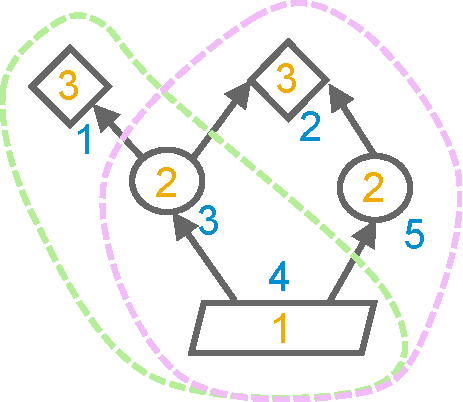
\includegraphics[width=0.30\textwidth]{Bilder/problem_illustration.pdf}
% 	\vspace{-10pt}
% 	% Das folgende ist ein Trick, um "Abbilgung x.y" in eine
% 	% eigene Zeile zu packen. Der Text zwischen [ und ] steht
% 	% im Abbildungsverzeichnis. Der Text darunter wird
% 	% tatsächlich angezeigt.
% 	\caption[Minimalbeispiel zur Teilgraph-Überspringungs-Problematik. Legende wie in \autoref{fig:trans_closures}.]{\unskip}
% 	Minimalbeispiel zur Teilgraph-Überspringungsproblematik. Legende wie in Abb. \ref{fig:trans_closures}.
% 	\label{fig:prob_illu}
% \end{wrapfigure}

% Leider lassen sich bei dem Vergleich zweier Submodelle gemeinsame Teilgraphen nicht gänzlich einsparen, indem der Similarity-Wert über Forks hinaus propagiert wird, um so jedem Knoten im Graph die Summe aller Knotenwerte unter ihm zuzuordnen, da ein gemeinsamer Teilgraph über mehrere Forks betreten werden kann (z.B. der Teilgraph der Schnittmenge von grün und lila in \autoref{fig:trans_closures} kann über Knoten 6 und 5 betreten werden) und nur der maximale Teilgraph gezählt werden darf - ansonsten würde es zu einer doppelten Wertung eines oder mehrerer Knoten kommen. Auch ist die Maximalität  des gemeinsamen Teilgraphen nur mit erheblichen Rechenaufwand, der dem Prinzip des Auslassens entgegensteht, zu überprüfen. Der Graph aus \autoref{fig:prob_illu} ist zur Veranschaulichung geeignet: Es ist schwierig Knoten 4 mit Wert 1 genau einmal zu zählen. Wird Knoten 3 betreten und der restliche Teilgraph (Knoten 4) übersprungen, so wird der Wert 3 zur Similarity addiert.

\chapter{Implementierung} 

Diese Kapitel beschäftigt sich mit der konkreten und detaillierten technischen Beschreibung 
der in Kapitel 3 \textit{Konzeption} vorgestellten Vorhaben, sodass die Experimente und deren Ergebnisse 
reproduziert werden können.


\section{Bewertungsmaße und Kostenfunktion} \label{sec:eval}


Als eine direkte und intuitiv sehr anschauliche Metrik zum Bewerten der Modellperformanz bei Segmentierungsproblemen
kann \ac{IoU} herangezogen werden. \\ 
Problematisch an der \ac{IoU} ist, dass alle möglichen Klassifikationen ($tp$, $fp$, $fn$, $tn$)
gleich stark gewichtet werden, wobei die wahr-positiven $tp$ zunächst Priorität haben sollten, 
während die Fehler der falsch-positiven $fp$ und falsch-negativen $fn$ im Gleichgewicht bleiben sollten, 
sodass es nicht zu einer trivialen Klassifikation als rein positiv oder rein negativ kommt. \\
Ein weiteres Problem ist, dass die \ac{IoU} sehr streng und intolerant gegenüber leichter Verschiebung der Erkennung 
bewertet. Wenn ein Fahrradweg, der nur wenige Pixel breit ist, um die Hälfte der Breite verschoben segmentiert würde, 
aber ansonsten komplett dem Radweg entspricht, würde die \ac{IoU} bereits von 1 auf 0,5 sinken, obwohl \textit{qualitativ} 
der Weg exakt erkannt wurde. Diese Intoleranz gegenüber leichter lokaler Verschiebung ist insbesondere in dem 
in dieser Arbeit vorgestellten BikeSat-Datensatz aus \autoref{sec:bike-data} problematisch, 
da dieser über \ac{OSM} annotiert ist und für viele Straßen die Lage des zugehörigen Radwegs geschätzt über 
die Spuranzahl ermittelt wird. \\
Das Problem lässt sich nicht umgehen, wenn dilatierte Bilder (vgl. \autoref{sec:eval:biou} \textit{BIoU}) verwendet werden.
Werden die Bilder dilatiert, ist die IoU auf diesen dilatierten Bildern gleich oder größer als auf den originalen Bildern. 
Diese neue dilatierte IoU erhöht aber auch die Anzahl an absolut Falsch-Positiven, was bei der BIoU nicht geschieht, 
weswegen gilt: $IoU \leq IoU_{dilatiert} \leq BIoU$. Allerdings ist die dilatierte IoU sehr schwierig zu interpretieren.
Während die IoU die strikte Überdeckung von Prediction zu Ground-Truth misst und die BIoU die gepufferte, also 
die Frage, ob die Prediction grob in der Nähe der Ground-Truth positioniert ist, beantwortet, misst die dilatierte IoU die strikte 
Überdeckung, als ob die Prediction und Ground-Truth umfangreicher, also die Radwege breiter wären. 
Diese Information ist neben der IoU und BIoU aber nicht sonderlich hilfreich, weswegen darauf verzichtet wird. \\ 
Aufgrund der genannten Einschränkungen ist die \ac{IoU} ungeeignet als Verlustfunktion, kann jedoch als ein Maß 
in die Bewertung der Modellperformanz mit einfließen. 

Dice gewichtet die $tp$ mehr als die \ac{IoU}. Damit wird das Ungleichgewichtsproblem vermindert und Dice ist 
besser geeignet als Verlustfunktion gegenüber der \ac{IoU}. Wie die \ac{IoU} hat Dice allerdings keine Toleranz 
gegenüber leichter Verschiebung der Radwege. Auf einem handannotierten Datensatz funktioniert Dice besser. 
Aufgrund der Beliebtheit von Dice in der semantischen Segmentierung 
wird ein guter Vergleich mit anderen Modellen ermöglicht. 
Aus diesen Gründen wird Dice für die Radwegerkennung als Verlustfunktion herangezogen.

\acf{BCE} wird für das originelle U-Net eingesetzt, ist aber in neueren U-Nets durch Dice abgelöst. 
Auch für das Problem der Radwegerkennung wird BCE nicht eingesetzt, da wie im originellen U-Net eine Weight-Map erstellt werden müsste, 
um das Klassenimbalanceproblem der BCE auszugleichen, was aber einen zu hohen Implementationsaufwand bedeuten würde, im Gegensatz zu 
Dice, welches ohne weiteren Aufwand funktioniert. 

\section{Implementation der Architekturen} \label{sec:arch-impl}

\subsection{Bike-U-Net} \label{sec:arch-impl:bunet}

Die konkrete Implementation der \acp{BUNet} erzielt die Vorgaben aus der Auflistung aus \autoref{sec:architecture:bike-u-net}. 
Nachfolgende Auflistung beschreibt detailliert, wie die \acp{BUNet} \ac{BUNet2} und \ac{BUNet15} umgesetzt sind.  

\begin{figure}
	\centering
	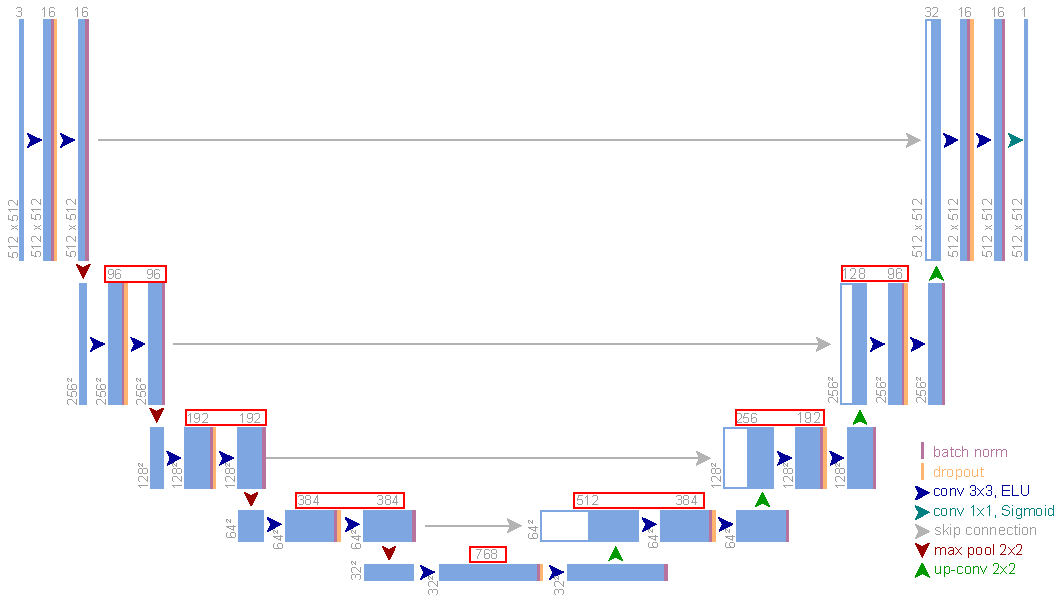
\includegraphics[width=1.\textwidth]{Bilder/own-unet-15mil-marked.pdf} 
	\caption{Bike-U-Net-15 mit 15,165 Mio. Parametern. Die geänderten Convolution-Filteranzahlen sind mit roten Kasten markiert.}
	\label{fig:bike-unet-15}
\end{figure} 

\begin{itemize}
	\item Zunächst werden Input-Bilder der Größe $width \times height \times 3$ verwendet. 
	Wobei $width$ und $height$ variabel in der Architektur sind, mit der Einschränkung, 
	dass diese Vielfache von 32 sein sollen, damit die mittlere Schicht nicht zu klein wird. 
	In jedem Fall wird ein Bild mit drei Kanälen (RGB) verwendet. 
	In der Abbildung ist exemplarisch $512 \times 512 \times 3$ gewählt. \\
	Der Output verwendet lediglich ein Output-Neuron pro Input-Pixel, wobei keine Aktivierung einen Hintergrundpixel 
	und eine Aktivieriung einen Radweg-Pixel impliziert, wie in \autoref{sec:state-of-the-art-roads} beschrieben. 
	\item Bei den Convolutional-Layern wird Padding eingesetzt,
	um die Dimensionen der Feature-Maps nicht nach und nach zu verkleinern und so einen exakt symmetrischen Aufbau zu gewährleisten.
	Ebenso wurde bei den Up-Convolutions Padding eingefügt, um auch hier eine Verkleinerung der Feature-Maps zu verhindern.
	Diese Anpassung wurde eingesetzt, um kein Zuschneiden bei den Skip-Connections zu benötigen, was die Lokalisierung verbessern soll,
	und so bei den in \autoref{sec:state-of-the-art-roads} beschriebenen Netzen gewöhnlich ist.
	\item 
	Im Bike-U-Net-2 beginnen die Filter bei 16 und verdoppeln sich bis 256, was zu ungefähr 2 Mio. 
	trainierbaren Parametern führt. Die Zahl an Parametern ist somit weitaus geringer als im 
	Original-U-Net (vgl. \autoref{sec:architekturkomponenten:unet}). \\
    Das \textit{\acf{BUNet15}} hat 15 Mio. Parameter (\autoref{fig:bike-unet-15} zeigt \ac{BUNet15}). Dies wird erzielt, 
	indem die Filteranzahl ab dem zweiten Block dreimal höher ist als in \ac{BUNet2}. So sind hier 16 Filter in Block eins, 
	dann 96 Filter in Block zwei, die sich verdoppeln bis hin zu 768 Filtern im mittleren Block und danach wieder halbieren bis zum vorletzten Block. 
	Dabei hat der letzte Block wieder 16 Filter. 
	Der erste und letzte Block haben jeweils 16 Filter, da damit der Rechen- und Speicheraufwand erheblich reduziert werden kann.
	Bis auf die Filteranzahl und die daraus resultierende Tiefe der Feature-Maps, sind \ac{BUNet2} und Bike-U-Net-15 identisch.
	\item Auf jede Convolution-Schicht folgt eine Batch-Normalization-Schicht. 
	\item Zusätzlich zu den Batch-Normalization-Schichten werden pro Block eine Dropout-Schicht 
	nach der jeweils ersten Convolution-Schicht eingezogen. Diese eröffnen den in \autoref{sec:hyperparameter:dropout} 
    beschriebenen Hyperparameter \textit{Dropout-Rate}.
	\item Die Convolution-Schichten werden durch \ac{ELU} (s. \autoref{sec:activation:elu}) aktiviert, 
	anstatt durch \ac{ReLU}, wie im Original-U-Net. 
	Hierdurch können die meisten der in \autoref{sec:activation} herausgearbeiteten Vorteile von \ac{ReLU},
	wie Robustheit gegen das Vanishing-Gradient-Problem, genutzt werden.  
	Um das Dying-Neuron-Problem zu adressieren, welches zu den in \autoref{sec:architekturkomponenten:unet} genannten Problemen führt, 
	wird auf \ac{ELU} (s. \autoref{sec:activation:elu}) zurückgegriffen, da damit alle Netzteile aktiv bleiben sollen. 
	Nachteil ist hierbei, dass die Berechnung von \ac{ELU} etwas aufwendiger ist. 
	Das Problem von unbeschränkt großen positiven Aktivierungen unter denen sowohl \ac{ELU} als auch \ac{ReLU} leiden,
	wird in diesem Netz durch die wiederholte automatische Standardisierung und Normalisierung durch die Batch-Norm-Schichten abgefedert.
	\item Für das Ouptut-Layer, nach der $1\times 1$-Convolution, wird die Sigmoid-Funktion verwendet. 
\end{itemize}

\subsection{VGG16-Bike-U-Net}

\textit{\ac{VBUNet}} nutzt das in \autoref{sec:pretrained-backbones:vgg16} beschriebene Netz VGG16 
mit auf ImageNet vortrainierten Gewichten als Backbone. \\
Hierzu werden die drei Fully-Connected-Layer 
(und Soft-Max-Aktivierung) am Ende entfernt und mit drei neuen \textit{conv3-512}-Schichten ersetzt. 
Diese bilden den mittleren (\enquote{untersten}) Block im U-Net. Darauf folgt eine direkte Spiegelung 
von VGG16 als Decoder mit abschließender $1\times 1$-Convolution. Im Gegensatz zum Bike-U-Net (s. \autoref{sec:architecture:bike-u-net}) 
und ursprünglichen U-Net (s. \autoref{sec:architekturkomponenten:unet}) werden allerdings keine 
\textit{Up-Conv3}-Layer mit trainierbaren Gewichten zum Upsampling genutzt, sondern 2D-Upsampling-Layer, 
ohne trainierbare Parameter. Diese Entscheidung wird getroffen, um VGG16 besser nachzuempfinden, 
da hier Maxpool-Schichten zum Downsampling verwendet werden, die ebenfalls keine trainierbaren Parameter enthalten.
Weiterhin sind nach jeder nicht-vortrainierten Convolution-Schicht, also nach jeder, die nicht zu VGG16 gehören, 
Batch-Normalization-Layer eingezogen, aus den in \autoref{sec:architecture:bike-u-net} und \autoref{sec:architekturkomponenten:batchnorm}
genannten Gründen wie schnellerem Training, leichter Glättung und fehlender sonstiger Standardisierung und Normalisierung.
Die für U-Net charakteristischen Skip-Connections werden vor jeder Maxpool-Schicht außer der ersten eingesetzt 
und mit dem korrespondierenden Decoder-Block verbunden. Dies resultiert in genau vier Skip-Connections, 
wie im Bike-U-Net und originellen U-Net. Abgeschlossen wird durch eine Sigmoid-Aktivierung, so wie im Bike-U-Net. \\
VGG16-Bike-U-Net enthält 23,7 Mio. Parameter. Grob die Hälfte davon (14,7 Mio.) sind von VGG16. 

\subsection{ResNet34-Bike-U-Net}

\textit{\ac{RBUNet}} nutzt das in \autoref{sec:pretrained-backbones:resnet} beschriebene Netz ResNet34 
mit auf ImageNet vortrainierten Gewichten als Backbone. 
Hierzu wird die eine Fully-Connected-Layer am Schluss des Netzes entfernt und mit einem Decoder ersetzt. 
Anders als bei \ac{VBUNet} ist der mittlere Block der U-Net-Struktur von ResNet34 
und nicht zusätzlich neu ergänzt. Grund dafür ist die höhere Anzahl an Parametern 
von ResNet34, welche ohne die Fully-Connected-Schicht bereits bei 24,4 Mio. liegt, im Gegensatz zu VGG16. 
Da der mittlere Block die meisten Parameter beinhaltet, wird keine weitere Vertiefung des Netzes vorgenommen,
um die Anzahl der Parameter nicht drastisch zu erhöhen. Anstelle dessen wird nach Ende der Convolution-Schichten von 
ResNet34 direkt mit dem Upsampling begonnen, welches wie bei \ac{VBUNet} mit Upsampling-Schichten 
bewerkstelligt wird. Auch wird im Widerspruch zu \ac{VBUNet} der Encoder - also ResNet34 - nicht gespiegelt, 
um eine Verdoppelung der Parameteranzahl zu vermeiden. Stattdessen wird ein einfacher, U-Net-ähnlicher Decoder
aus fünf Blöcken á Upsampling-Schicht und zwei Convolution-Schichten verwendet, wobei in jedem Block 
die Filter-Anzahl von 512 an bis schließlich 16 halbiert wird. Abgeschlossen wird wie bei \ac{VBUNet} und
\ac{BUNet} mit $1\times 1$-Convolution und Sigmoid-Aktivierung. Aus den gleichen Gründen wie bei \ac{VBUNet}
sind nach jeder Convolution-Schicht Batch-Normalization-Schichten eingezogen. 
Es erfolgt wiederum das Einsetzen von vier Skip-Connection nach U-Net-Vorbild ergänzend zu den 
Skip-Connections der Residuen-Blöcke an folgenden Stellen: 
nach der $7\times 7$-Convolution zu Beginn von ResNet34, 
am Ende der Blöcke mit 64 Filter, am Ende der Blöcke mit 128 Filtern 
und am Ende der Blöcke mit 256 Filtern. Im Decoder werden diese jeweils 
zu Beginn der ersten vier Decoder-Blöcke konkateniert. \\ 
ResNet34-Bike-U-Net enthält 24,4 Mio. Parameter. Davon sind 21,2 Mio. von ResNet34 und lediglich 3,2 Mio. 
vom Decoder, welcher somit eher unterrepräsentiert ist im Netz.  

\subsection{DenseNet121-Bike-U-Net}

\textit{\ac{DBUNet}} nutzt das in \autoref{sec:pretrained-backbones:densenet121} beschriebene Netz DenseNet121 
mit auf ImageNet vortrainierten Gewichten als Backbone.
Hierzu wird der Classification-Layer bestehend aus einer $7\times 7$-Average-Pool-Schicht 
und einer Fully-Connected-Layer entfernt und durch einen Decoder ersetzt. 
Wie schon bei \ac{RBUNet} erstreckt sich das DenseNet bis in den mittleren U-Net-Block. Beim \ac{DBUNet} 
liegt der Grund dafür allerdings nicht in der hohen Parameterzahl, sondern in der hohen sonstigen Komplexität 
des Netzes. So benötigt DenseNet121 trotz deutlich geringerer Parameterzahl für die Inferenz und das Training länger 
als sowohl \ac{RBUNet}, als auch \ac{VBUNet}. Vermutlich ist hierfür die große Tiefe von 64 Schichten, wovon 
60 Convolution-Schichten sind, verantwortlich. Um die Inferenz- und Trainingszeit nicht weiter zu belasten, 
ist der Decoder eher simpel gehalten, enthält also wenig Parameter. Für den Decoder wird die gleiche Architektur wie im \ac{RBUNet} verwendet.
Auch hier sind die Batch-Normalization-Schichten eingezogen. Der Unterschied besteht darin, 
dass die erste Convolution-Schicht anders als bei \ac{RBUNet} nicht von 512 Kanälen auf 256 abbildet, 
sondern von 1536 auf 256. Dies liegt an der Konkatenierung der DenseNet-Architektur. Wieder wird das 
Netz abgeschlossen durch eine $1\times 1$-Convolution gefolgt von einer Sigmoid-Aktivierung. 
Auch hier werden wieder vier Skip-Connections eingebaut, um die U-Net-Architektur nachzuahmen. 
Diese Skip-Connections sind im Falle von \ac{DBUNet} im Encoderteil nach der ersten $7 \times 7$-Convolution 
und dann jeweils nach jeder weiteren $1\times 1$-Convolution der DenseNet-Transition-Zonen eingesetzt. 
Im Decoder-Teil sind diese wie bei \ac{RBUNet} zu Beginn jedes Decoder-Blocks bis auf den letzten eingebaut. \\
DenseNet121-Bike-U-Net enthält 12,1 Mio. Parameter, wovon 6,9 Mio. zum DenseNet121 und 5,1 Mio. neu hinzugefügt 
wurden. Trotz doppelter bzw. sogar vierfacher Tiefe besteht \ac{DBUNet} nur aus ungefähr halb so vielen 
Parametern wie \ac{RBUNet} und \ac{VBUNet}. 


% Zunächst wird eine Basisimplementation gegeben, die den Algorithmus zur Subproblemerzeugung und Similarity-Berechnung aus \autoref{sec:alg_comp} umsetzt und diesen dann auf Geschwindigkeit optimiert.

% \section{Basisimplementation}

% \begin{algorithm}
% 	\caption{Vereinfachter Algorithmus zum Erstellen der Subprobleme aus den Submodellen}\label{lst:create_sub}
% 	\begin{algorithmic}[1]
% 		\Procedure{Create Subproblems}{$F$} 
% 			\For{$S \in atomicSubmodels$}
% 				\State $S.graph \gets calculateGraph(S)$
% 				\State $S.graph \gets reduceGraph(S.graph, F)$
% 			\EndFor \Comment{$n := |atomicSubmodels|$}
% 			\While{$|atomicSubmodels| \neq 0$} \Comment{$O(\frac{n(n+1)}{2}) \cdot O(t_{sim}) = O(n^2 \cdot t_{sim})$}
% 				\State $M \gets selectOne(atomicSubmodels)$
% 				\State $M.set \gets \emptyset$
% 				\While{$complexity(M) < minSubproblemComplexity$}
% 					\State $highestSim \gets -1$					
% 					\For{$S \in atomicSubmodels$}
% 						\State $sim \gets computeSim(M, S)$
% 						\If{$sim > highestSim$}
% 							\State $mostSimilar \gets S$
% 							\State $highestSim \gets sim$
% 						\EndIf
% 					\EndFor
% 					\State $M \gets M \cup mostSimilar$
% 					\State $M.set \gets M.set \cup mostSimilar.set$
% 					\State $atomicSubmodels \gets atomicSubmodels \setminus mostSimilar$
% 				\EndWhile
% 				\State $subproblems \gets subproblems \cup \{M\}$
% 			\EndWhile		
% 		\EndProcedure
% 	\end{algorithmic}
% \end{algorithm}


\chapter{Ergebnisse} \label{sec:results}

Das Kapitel stellt die Ergebnisse der Tests der verschiedenen Modelle dar. Außerdem 
wird eine Übersicht über die benötigte Trainingszeit für die Modelle gegeben. 

\section{Benötigte Trainingszeit}

\begin{itemize}
    \item Eine Epoche des Pre-Trainings auf dem Combined-Straßendatensatz dauert zwischen 40 und 50 Minuten. 
    \item Eine Epoche des Trainings auf dem BikeSat-Datensatz dauert zwischen 10 und 17 Minuten. 
    \item Die Netze konvergieren nach circa 33-57 Epochen auf beiden Datensätzen. 
    \item Das Training wird immer vorzeitig vor dem Ablaufen der 100 Epochen beendet.
    \item Der zeitliche Mehraufwand durch die Bild-Augmentierung während des Trainings (vgl. \autoref{sec:pre-processing}) 
    liegt im Schnitt bei 3 min 30s pro Epoche für beide Augmentierungsmethoden (Basic-Augmentation und Color-Augmentation).  
\end{itemize}

\section{Pre-Training-Ergebnisse zur Straßenerkennung}

\begin{table}[ht]
	\centering
	\begin{tabular}{l|c|c}
		Modell & \ac{IoU} & \ac{BIoU} \\
		\midrule
        BUNet2 & 57,13 & 76,71 \\ 
        BUNet15 & 60,75 & 80,80 \\ 
        VBUNet & \textbf{64,26} & \textbf{85,64} \\ 
        RBUNet & 61,45 & 83,86 \\ 
        DBUNet & 62,56 & 84,46 \\ 
        
	\end{tabular}
	\caption{Ergebnisse des Pre-Trainings der Modelle auf der Testpartition des Combined-Datensatzes in Prozent.}
	\label{tab:results-roads}
\end{table}

\begin{figure}
	\centering
	\begin{minipage}{.41\textwidth}
		\centering
		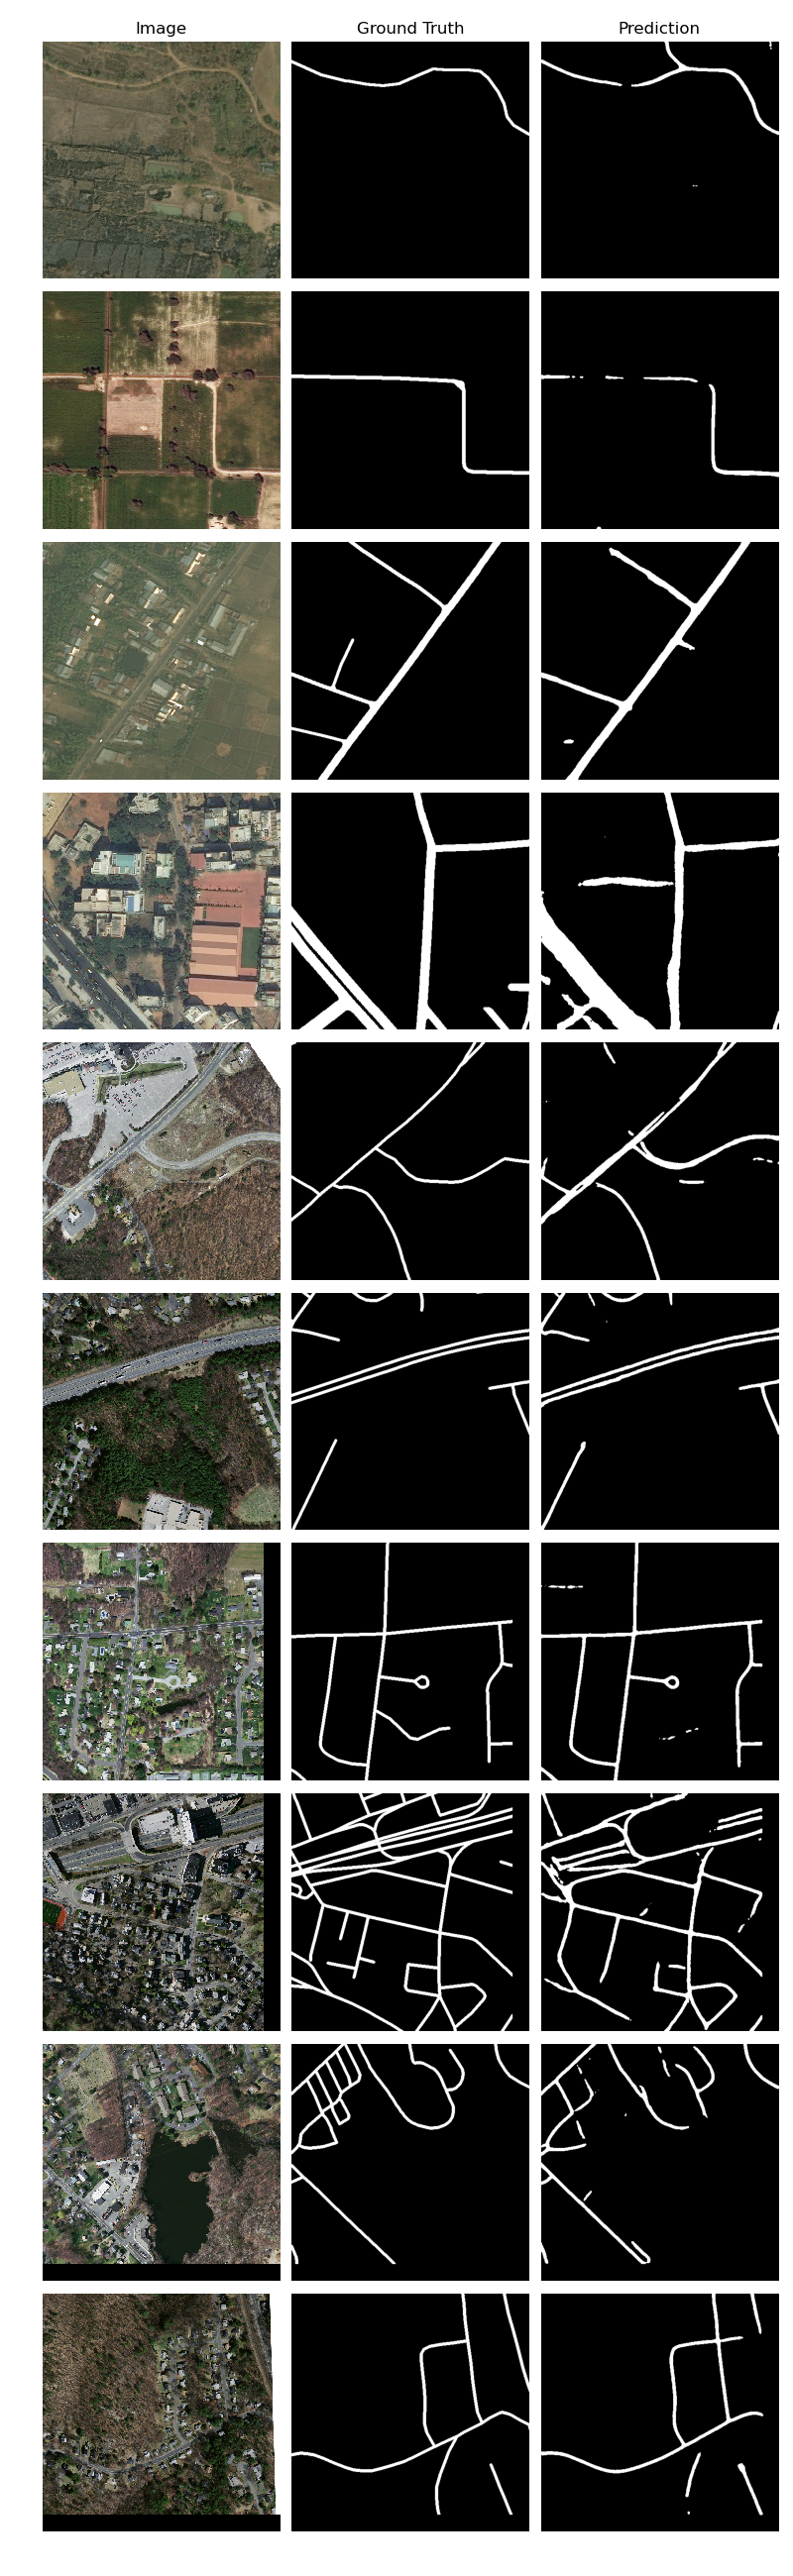
\includegraphics[width=1.\linewidth]{Bilder/Samples-Combined/bunet2.png}
	\end{minipage}
	\begin{minipage}{.41\textwidth}
		\centering
		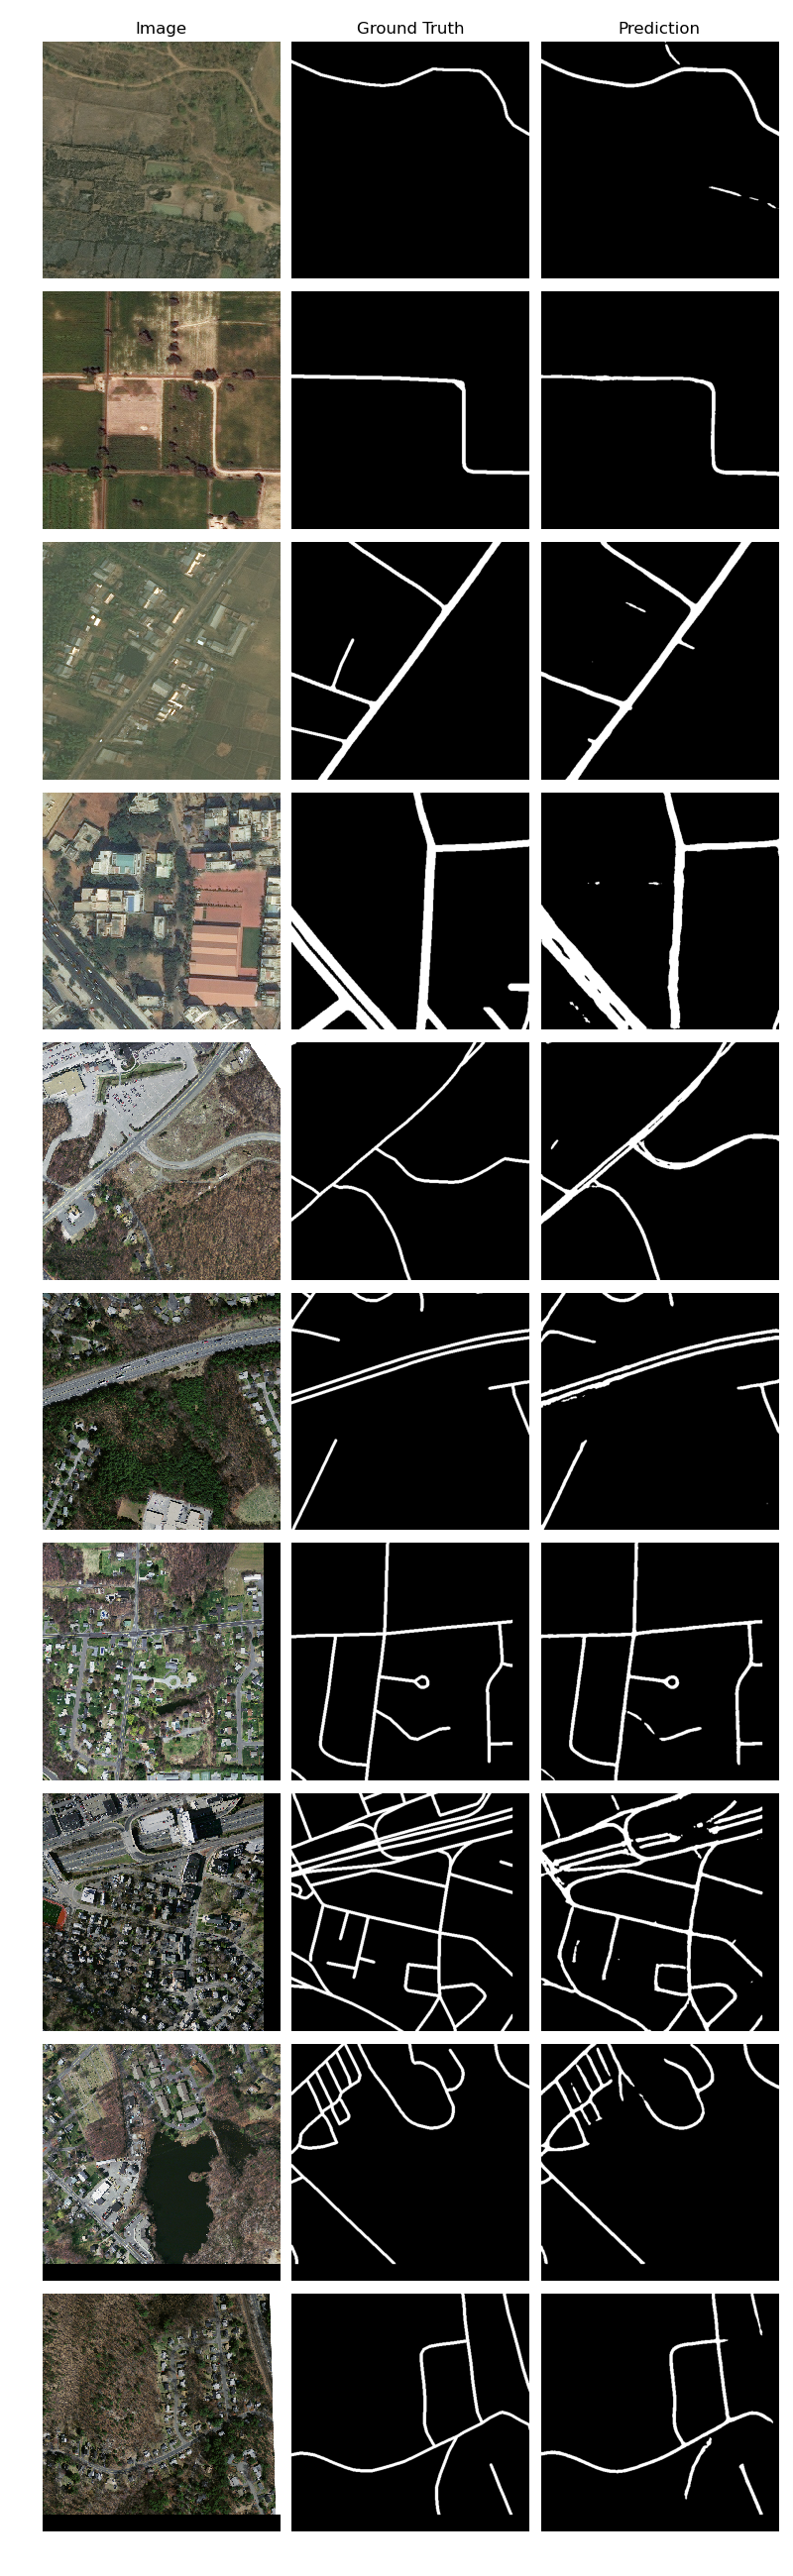
\includegraphics[width=1.\linewidth]{Bilder/Samples-Combined/vbunet.png}
	\end{minipage}

	\caption{Beispiel-Predictions des $BUNet2$ (links) und $VBUNet$ (rechts) auf dem Combined-Datensatz.}
	\label{fig:combined-samples-bune2-vbunet}
\end{figure}

\autoref{tab:results-roads} zeigt die Test-Ergebnisse der Modelle nach Training auf dem Combined-Datensatz 
(vgl. \autoref{sec:pre-training-roads}) in Prozent. Pro Spalte ist das höchste Ergebnis hervorgehoben. 
\ac{BUNet2} und \ac{BUNet15} sind von Grund auf trainiert, während \ac{VBUNet}, \ac{RBUNet} und \ac{DBUNet} einen auf 
ImageNet vortrainierten Encoder aufweisen. Die \ac{BIoU} verwendet wie bei der Radwegerkennung und wie in \autoref{sec:eval:biou} 
festgelegt eine Puffergröße von 15 Pixeln. 

\autoref{fig:combined-samples-bune2-vbunet} zeigt ausgewählte Beispielpredictions des \ac{BUNet2} (links) und 
des \ac{VBUNet}.\footnote{Weitere Beispiele anderer Netze in \autoref{sec:pred-combined}.}

\section{Ergebnisse der Radwegerkennung}

\begin{table}[ht]
	\centering
	\begin{tabular}{l|cc|cc|cc|cc}
		& \multicolumn{4}{c|}{Basic Augmentation} & \multicolumn{4}{c}{Color Augmentation} \\
        & \multicolumn{2}{c|}{BikeSat} & \multicolumn{2}{c|}{Karlsruhe} & \multicolumn{2}{c|}{BikeSat} & \multicolumn{2}{c}{Karlsruhe} \\
		Modell & \ac{IoU} & \ac{BIoU} & \ac{IoU} & \ac{BIoU} & \ac{IoU} & \ac{BIoU} & \ac{IoU} & \ac{BIoU} \\
		\midrule
        BUNet2$^*$ & 23,54 & 47,71 & 01,30 & 34,80 &  27,47 & 55,19 & 12,69 & 47,53 \\
        BUNet2$^l$ & 24,48 & 51,77 & 02,19 & 12,11 &  28,06 & 57,21 & 08,54 & 39,19 \\
        BUNet2$^r$ & 25,35 & 51,27 & 09,36 & 47,57 &  25,95 & 53,73 & 04,56 & 25,97 \\
		\midrule

        BUNet15$^*$ & 27,93 & 56,55 & \textbf{21,52} & \textbf{59,25} &  30,80 & 59,99 & 06,84 & 33,23 \\
        BUNet15$^l$ & 28,14 & 57,14 & 16,47 & 54,17 &  30,98 & 60,50 & 07,47 & 30,20 \\
        BUNet15$^r$ & 28,22 & 57,26 & 10,17 & 53,81 &  29,95 & 59,46 & 08,23 & 26,82 \\
		\midrule

        VBUNet$^*$ & 30,45 & 61,48 & 09,69 & 37,84 &  \textbf{31,71} & \textbf{61,32} & 09,29 & 31,15 \\
        VBUNet$^l$ & \underline{\textbf{32,24}} & \textbf{62,93} & 12,85 & 54,91 &  21,91 & 45,88 & 03,19 & 23,25 \\
        VBUNet$^r$ & \textbf{31,84} & 61,51 & 17,53 & \textbf{61,51} &  25,65 & 51,82 & 10,74 & 32,31 \\
		\midrule

        RBUNet$^*$ & 29,11 & 60,53 & 11,74 & 32,80 &  \underline{\textbf{33,54}} & \underline{\textbf{65,02}} & \textbf{23,24} & \textbf{65,71} \\
        RBUNet$^l$ & 30,98 & 60,51 & \underline{\textbf{24,67}} & \underline{\textbf{65,27}} &  29,32 & 59,83 & 09,67 & 53,08 \\
        RBUNet$^r$ & 31,31 & \underline{\textbf{63,55}} & \textbf{18,21} & 55,53 &  29,42 & 59,58 & \underline{\textbf{34,66}} & \underline{\textbf{68,26}} \\
		\midrule

        DBUNet$^*$ & 30,76 & 61,78 & 07,14 & 45,97 &  \textbf{32,24} & \textbf{64,77} & 14,64 & 50,02 \\
        DBUNet$^l$ & 31,55 & 62,38 & 17,47 & 55,20 &  29,64 & 60,47 & 14,83 & 51,19 \\
        DBUNet$^r$ & \textbf{32,12} & \textbf{62,99} & 14,03 & 51,73 &  30,30 & 61,24 & 17,43 & \textbf{62,28} \\
        
	\end{tabular}
	\caption{Ergebnisse der Modelle auf der Testpartition des BikeSat-Datensatzes und dem Karlsruhe-Datensatz
	für beide Augmentierungsmethoden. 
    In Prozent.}
	\label{tab:results}
\end{table}

\autoref{tab:results} zeigt die Test-Ergebnisse der Modelle nach Training (s. \autoref{sec:training} für Details) auf dem BikeSat-Datensatz 
(s. \autoref{sec:bike-data}) für jede Augmentierungsmethode (Basic- u. Color-Augmentation) während des Trainings in Prozent. 
Zusätzlich zeigt die Tabelle die Test-Ergebnisse auf allen 196 $512{\times}512$-Ausschnitten 
des Karlsruhe-Datensatz (s. \autoref{sec:karlsruhe}) in Prozent. Der Karlsruhe-Datensatz in dieser Tabelle
enthält auch Ausschnitte, die \textit{keine} Radwege enthalten. \\ 
Pro Spalte sind die höchsten drei Ergebnisse hervorgehoben und das höchste unterstrichen.
Die \ac{BIoU} hat eine Puffergröße von 15 Pixeln, wie in \autoref{sec:eval:biou} festgelegt.\\


\begin{table}[ht]
	\centering
	\begin{tabular}{l|cc|cc|cc}
        & \multicolumn{2}{c|}{\textcolor{gray}{BikeSat}} & \multicolumn{2}{c|}{\textcolor{gray}{Karlsruhe}} & \multicolumn{2}{c}{Wolfsburg} \\
		Modell & \textcolor{gray}{\ac{IoU}} & \textcolor{gray}{\ac{BIoU}} & \textcolor{gray}{\ac{IoU}} & \textcolor{gray}{\ac{BIoU}} & \ac{IoU} & \ac{BIoU} \\
		\midrule
        BUNet2$^*$ & \textcolor{gray}{27,47} & \textcolor{gray}{55,19} & \textcolor{gray}{12,69} & \textcolor{gray}{47,53} &  28,44 & 57,30 \\
        BUNet2$^l$ & \textcolor{gray}{28,06} & \textcolor{gray}{57,21} & \textcolor{gray}{08,54} & \textcolor{gray}{39,19} &  29,92 & 59,64 \\
        BUNet2$^r$ & \textcolor{gray}{25,95} & \textcolor{gray}{53,73} & \textcolor{gray}{04,56} & \textcolor{gray}{25,97} &  28,62 & 57,98 \\
		\midrule

        BUNet15$^*$ & \textcolor{gray}{30,80} & \textcolor{gray}{59,99} & \textcolor{gray}{06,84} & \textcolor{gray}{33,23} &  30,68 & 61,86 \\
        BUNet15$^l$ & \textcolor{gray}{30,98} & \textcolor{gray}{60,50} & \textcolor{gray}{07,47} & \textcolor{gray}{30,20} &  31,31 & 61,71 \\
        BUNet15$^r$ & \textcolor{gray}{29,95} & \textcolor{gray}{59,46} & \textcolor{gray}{08,23} & \textcolor{gray}{26,82} &  30,99 & 60,84 \\
		\midrule

        VBUNet$^*$ & \textcolor{gray}{\textbf{31,71}} & \textcolor{gray}{\textbf{61,32}} & \textcolor{gray}{09,29} & \textcolor{gray}{31,15} &  \textbf{32,90} & \textbf{66,08} \\
        VBUNet$^l$ & \textcolor{gray}{21,91} & \textcolor{gray}{45,88} & \textcolor{gray}{03,19} & \textcolor{gray}{23,25} &  22,79 & 50,18 \\
        VBUNet$^r$ & \textcolor{gray}{25,65} & \textcolor{gray}{51,82} & \textcolor{gray}{10,74} & \textcolor{gray}{32,31} &  27,53 & 56,97 \\
		\midrule

        RBUNet$^*$ & \textcolor{gray}{\underline{\textbf{33,54}}} & \textcolor{gray}{\underline{\textbf{65,02}}} & \textcolor{gray}{\textbf{23,24}} & \textcolor{gray}{\textbf{65,71}} &  \underline{\textbf{34,42}} & \textbf{67,74} \\
        RBUNet$^l$ & \textcolor{gray}{29,32} & \textcolor{gray}{59,83} & \textcolor{gray}{09,67} & \textcolor{gray}{53,08} &  30,80 & 63,30 \\
        RBUNet$^r$ & \textcolor{gray}{29,42} & \textcolor{gray}{59,58} & \textcolor{gray}{\underline{\textbf{34,66}}} & \textcolor{gray}{\underline{\textbf{68,26}}} &  31,17 & 63,47 \\
		\midrule

        DBUNet$^*$ & \textcolor{gray}{\textbf{32,24}} & \textcolor{gray}{\textbf{64,77}} & \textcolor{gray}{14,64} & \textcolor{gray}{50,02} &  \textbf{33,70} & \underline{\textbf{68,48}} \\
        DBUNet$^l$ & \textcolor{gray}{29,64} & \textcolor{gray}{60,47} & \textcolor{gray}{14,83} & \textcolor{gray}{51,19} &  31,02 & 63,21 \\
        DBUNet$^r$ & \textcolor{gray}{30,30} & \textcolor{gray}{61,24} & \textcolor{gray}{\textbf{17,43}} & \textcolor{gray}{\textbf{62,28}} &  31,48 & 64,48 \\
        
	\end{tabular}
	\caption{Ergebnisse der Modelle auf dem Wolfsburg-Datensatz mit farbverändernden Augmentierungen (Color-Aug.). In Prozent.
	(Die Ergebnisse von BikeSat und Karlsruhe entsprechen \autoref{tab:results} und sind zur einfacheren Vergleichbarkeit erneut aufgeführt.)}
	\label{tab:results-wolfsburg}
\end{table}

\autoref{tab:results-wolfsburg} ergänzt \autoref{tab:results} um die Ergebnisse auf dem Wolfsburg-Datensatz für 
Training mit Color-Augmentation. Zur besseren Übersichtlichkeit sind die Ergebnisse für Basic-Aug. hier ausgespart, 
da diese weniger interessant sind. 
\begin{enumerate}
	\item Es fällt auf, dass sowohl die \ac{IoU} als auch die \ac{BIoU} für alle Modelle
	auf dem Wolfsburg-Datensatz besser ist, als auf der Testpartition des BikeSat-Datensatzes.  
	Selbiges gilt für den Vergleich von Wolfsburg mit Karlsruhe, bis auf die Modelle VBUNet$^l$ und 
	RBUNet$^r$, die auf dem Karlsruhe-Datensatz in IoU sowie BIoU höhere Werte erzielen, als auf dem Wolfsburg-Datensatz.
	\item Über alle Datensätze performt RBUNet$^*$ am besten. Es liefert über alle sechs Maßzahlen Top-3-Ergebnisse wobei es 
	in für drei davon am besten performt. 
	\item Darüber hinaus ist auffällig, wie viel schlechter die vortrainierten Varianten der VBUNet-Architektur performen. 
	Während VBUNet$^*$ auf dem BikeSat- und Wolfsburg-Datensatz solide Ergebnisse liefert, liegen VBUNet$^l$ und VBUNet$^r$ 
	weit unterhalb. Bei der IoU 10 Prozentpunkte, bei der BIoU bis zu 16 Prozentpunkte.
	\item Generell performen die Netze der \ac{BUNet2}-Architektur schlechter als die der \ac{BUNet15}-Architektur.
	\item Interessanterweise performen die vortrainierten Modelle der Backbone-Architekturen auf dem BikeSat- und 
	Wolfsburg-Datensatz konstant schlechter als die nicht vortrainierten. Die rechtsseitig vortrainierten zeigen 
	allerdings bessere Performance auf dem Karlsruhe-Datensatz als die anderen Modelle der jeweiligen Backbone-Archtiektur.\\
	Für Modelle der BUNet-Architektur sind die Ergebnisse recht ähnlich und es ist keine schlechtere Performance
	zu beobachten. 
\end{enumerate}


\subsection{Beispiel-Predictions ausgewählter Netze}

\autoref{fig:bikesat-samples-bunet2-s-vbunet-l} zeigt ausgewählte Beispielpredictions des $BUNet2^*$ (a) und 
des $VBUNet^l$ (b) auf dem BikeSat-Datensatz bei Training mit Basic-Augmentation.\footnote{Weitere Beispiele anderer Netze in \autoref{sec:pred-bikesat}.}

\autoref{fig:ka-samples-rbunet-l-rbunet-s} zeigt ausgewählte Beispielpredictions des $RBUNet^l$ (a) und 
des $RBUNet^*$ (b) auf dem Karlsruhe-Datensatz bei Training mit Basic-Augmentation.\footnote{Weitere Beispiele anderer Netze in \autoref{sec:pred-karlsruhe}.}

\autoref{fig:ka-samples-rbunet-l-rbunet-s-color} zeigt ausgewählte Beispielpredictions des $RBUNet^l$ (a) und 
des $RBUNet^*$ (b) auf dem Karlsruhe-Datensatz bei Training mit Color-Augmentation.

\autoref{fig:wolfsburg-samples-rbunet-l-rbunet-s-color} zeigt ausgewählte Beispielpredictions des $RBUNet^l$ (a) und 
des $RBUNet^*$ (b) auf dem Wolfsburg-Datensatz bei Training mit Color-Augmentation.

\begin{figure}[h]
	\centering
	\begin{subfigure}{.4\textwidth}
		\centering
		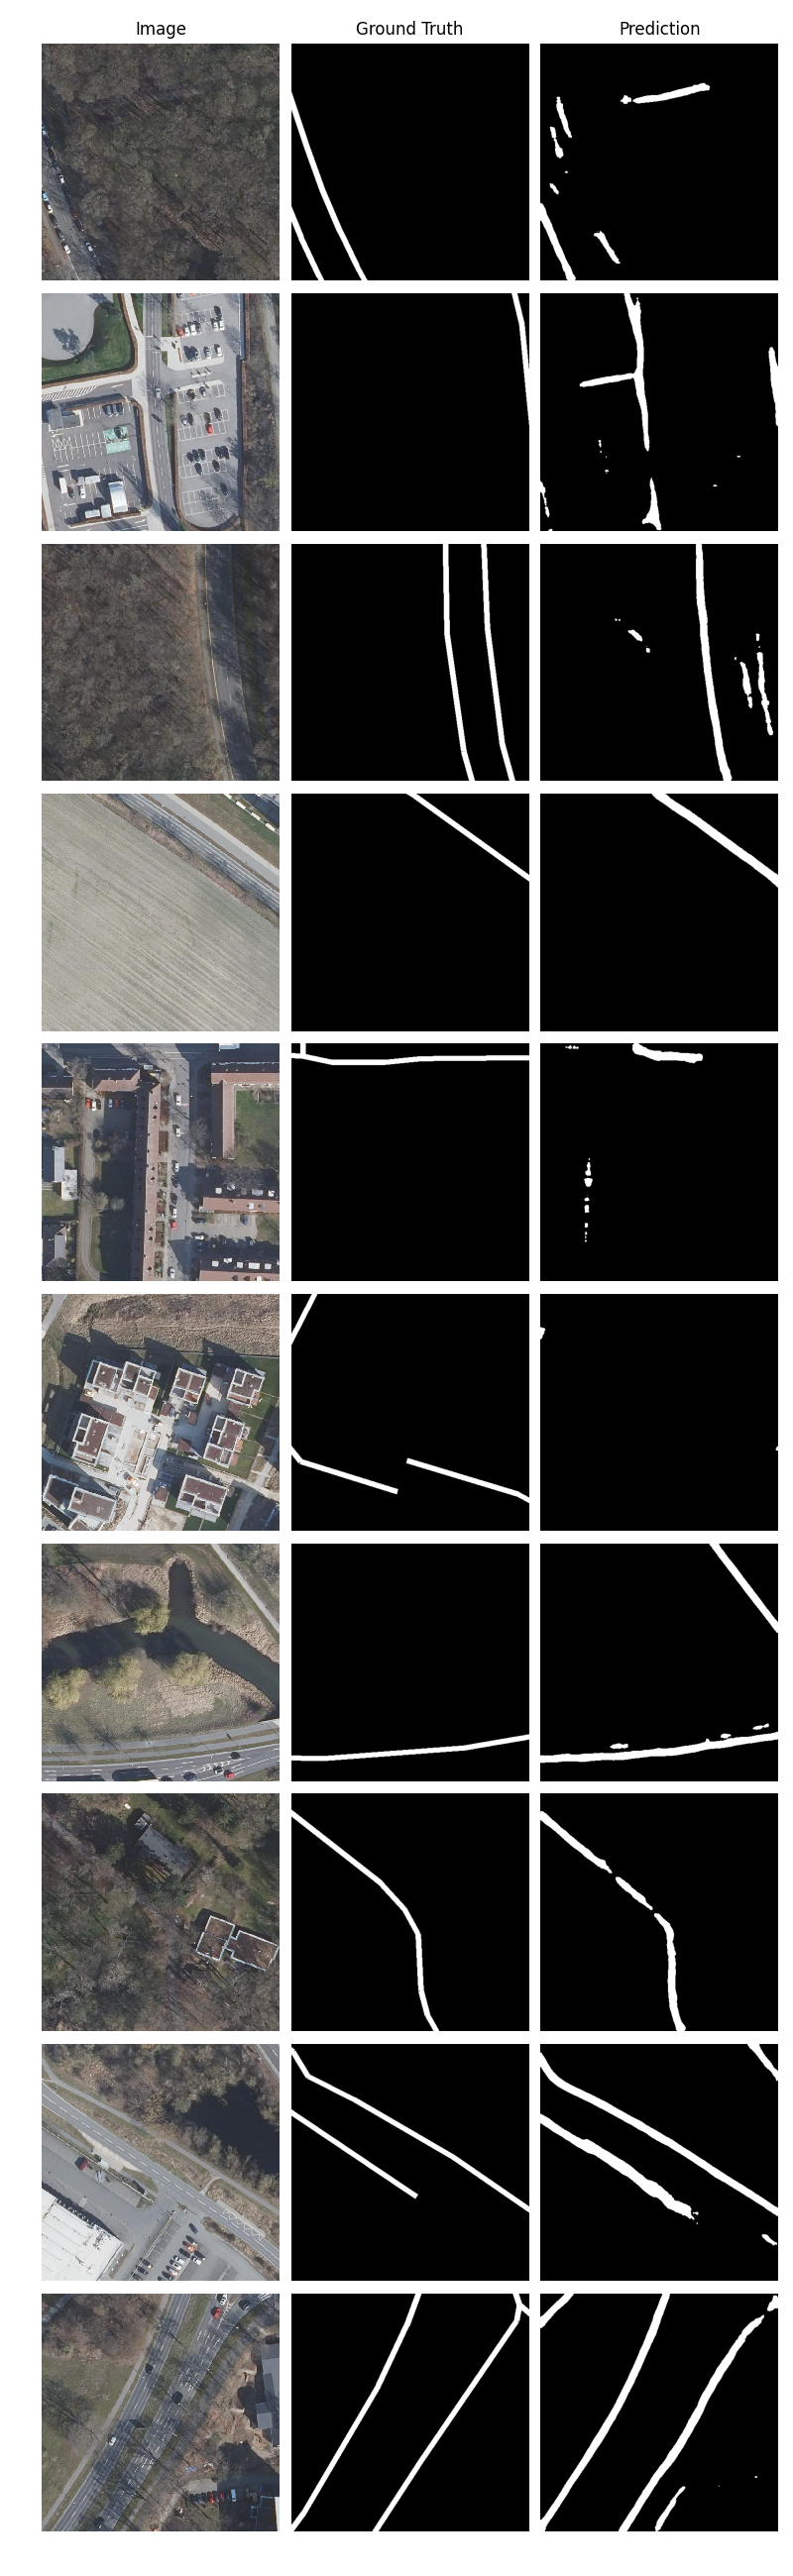
\includegraphics[width=1.\linewidth]{Bilder/Samples-Bikesat/bunet2-s.png}
		\caption{}
	\end{subfigure}
	\begin{subfigure}{.4\textwidth}
		\centering
		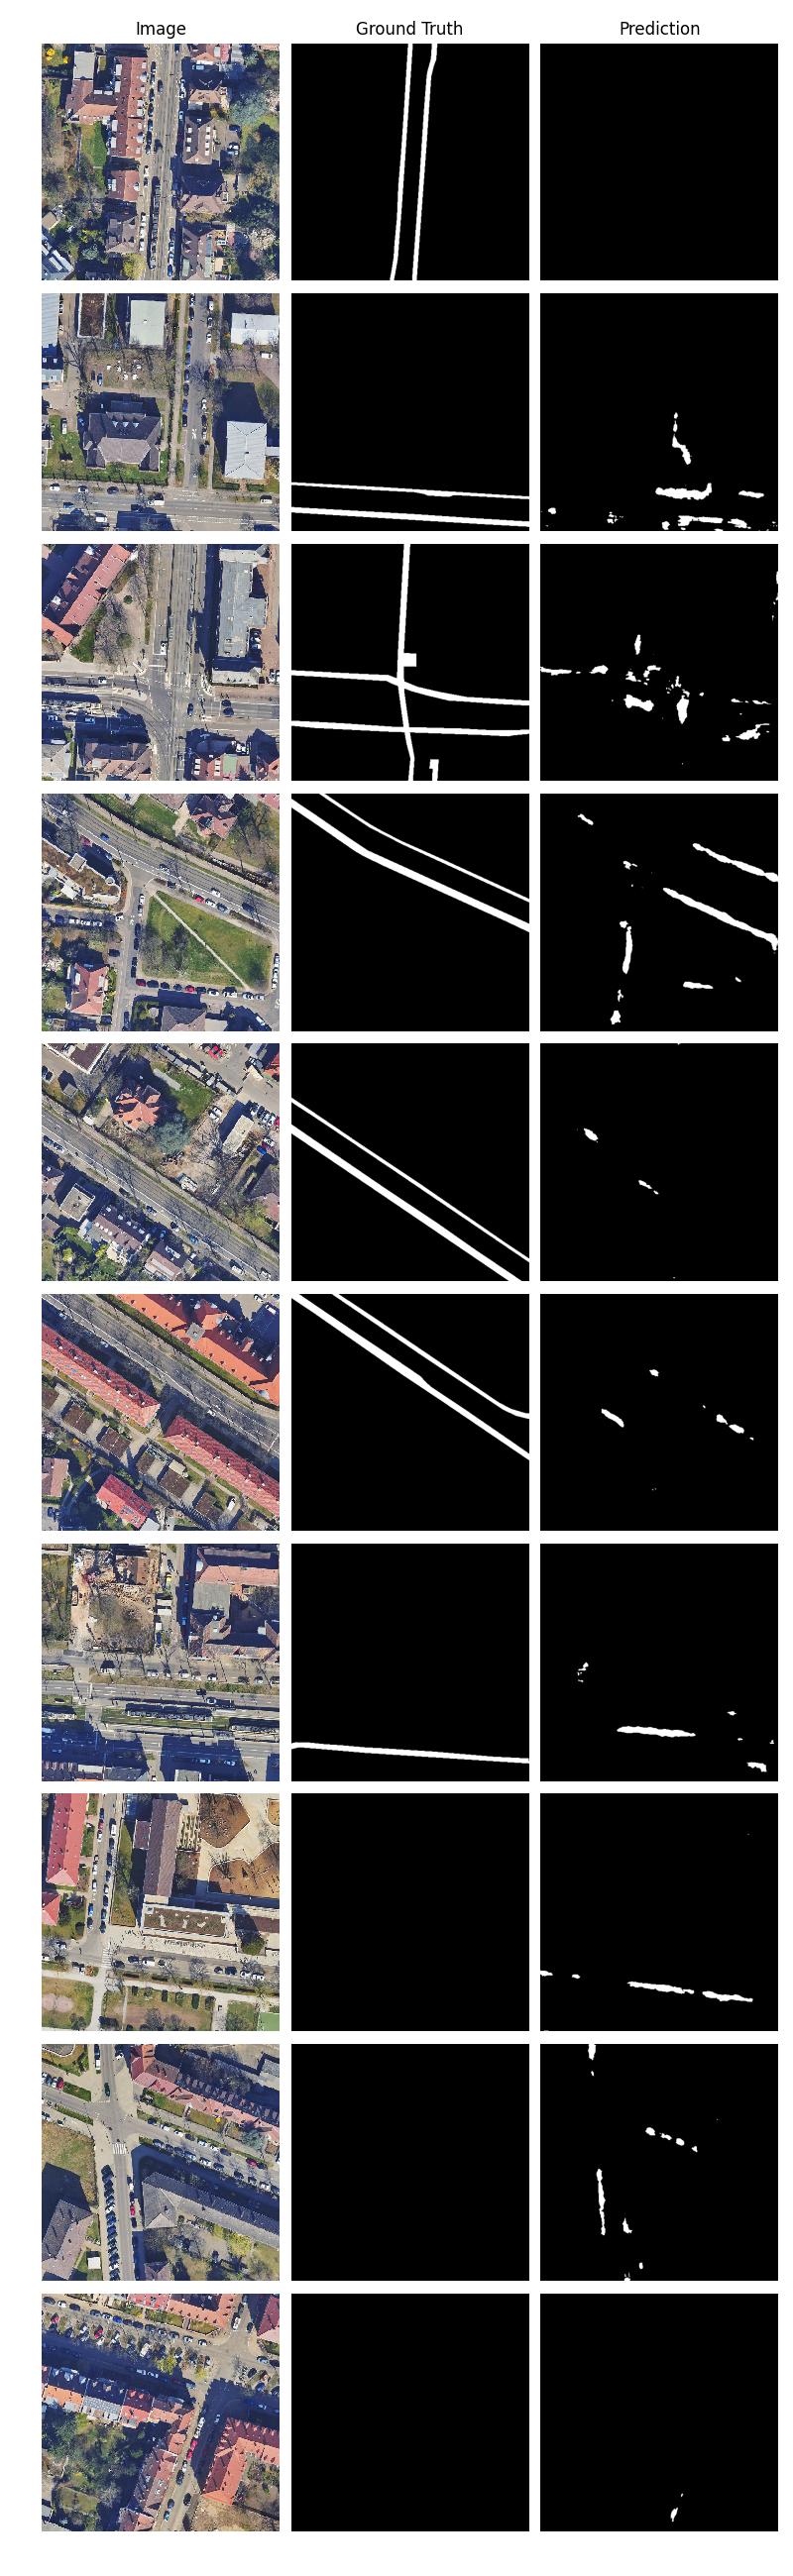
\includegraphics[width=1.\linewidth]{Bilder/Samples-Bikesat/vbunet-l.png}
		\caption{}
	\end{subfigure}

	\caption{Beispiel-Predictions des $BUNet2^*$ (a) und $VBUNet^l$ (b) auf dem BikeSat-Datensatz trainiert mit \textit{Basic}-Augmentation.}
	\label{fig:bikesat-samples-bunet2-s-vbunet-l}
\end{figure}

\begin{figure}[h]
	\centering
	\begin{subfigure}{.4\textwidth}
		\centering
		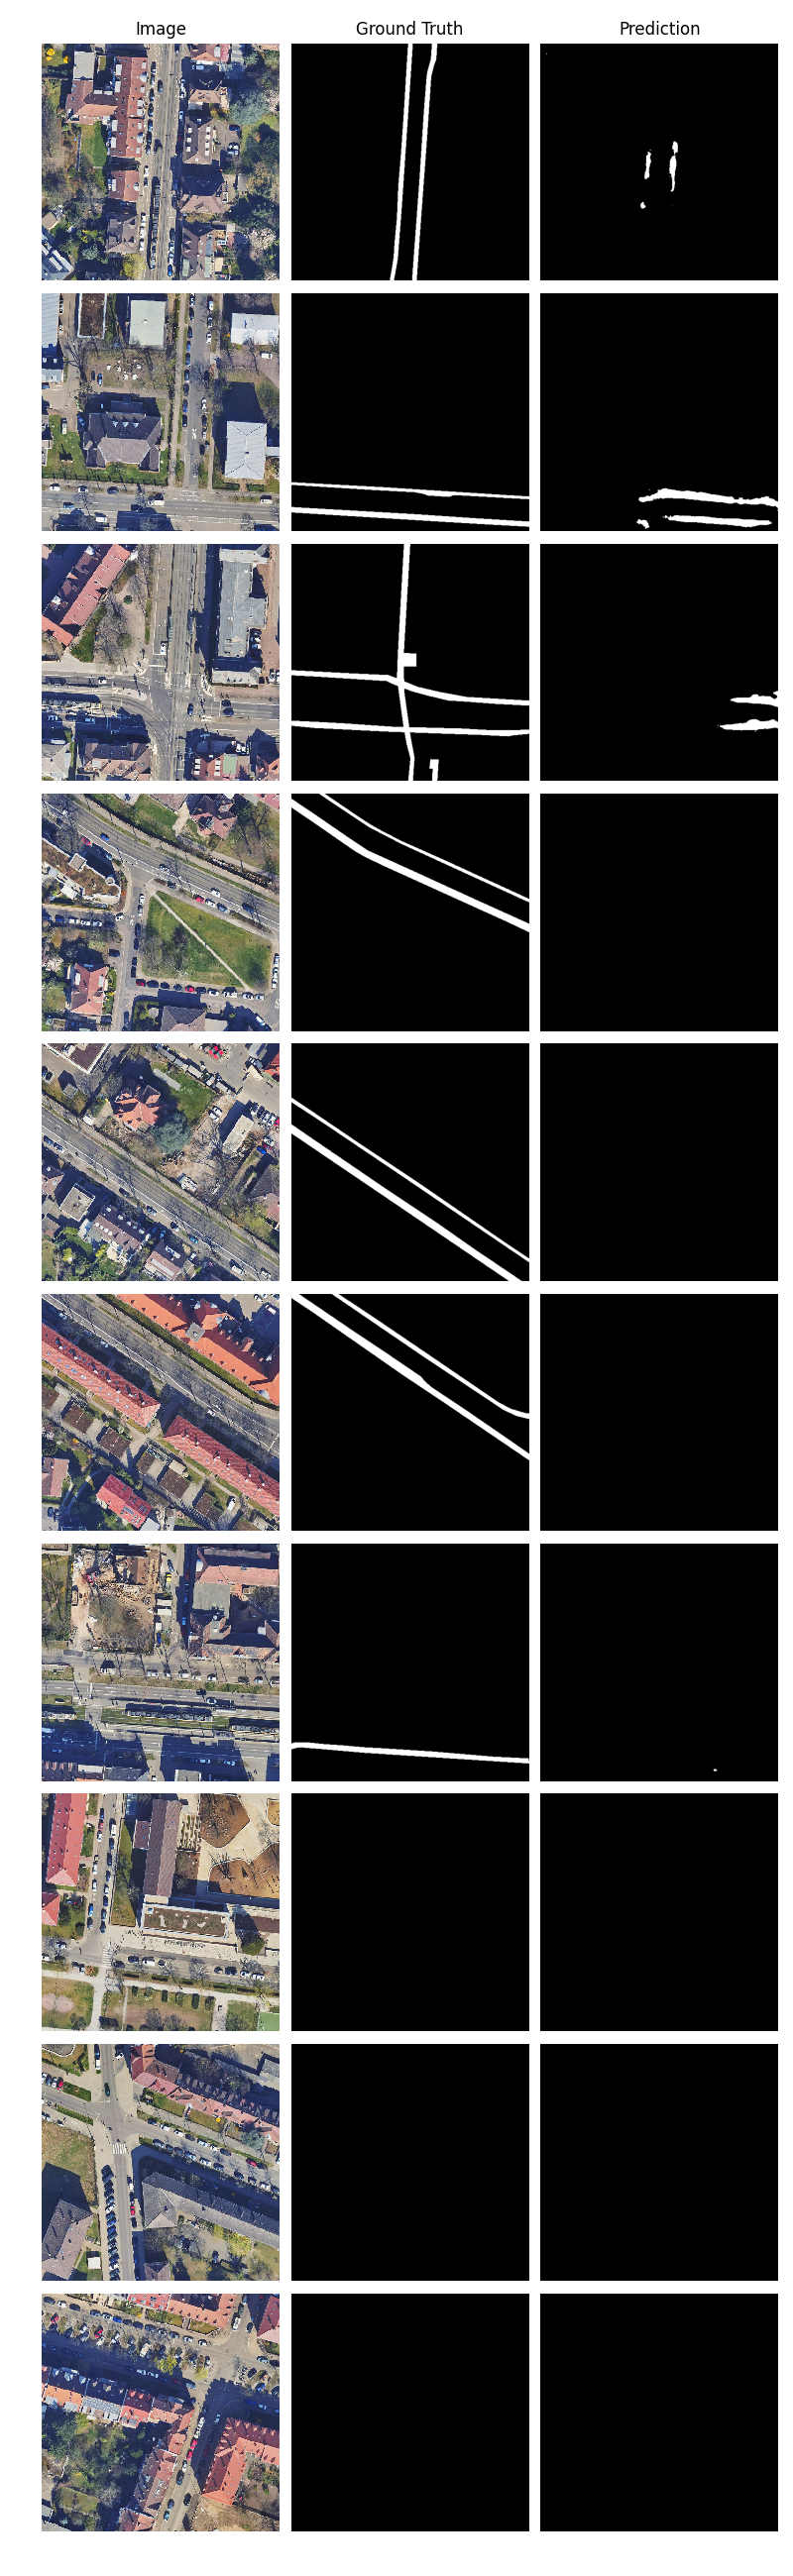
\includegraphics[width=1.\linewidth]{Bilder/Samples-KA/rbunet-l.png}
		\caption{}
	\end{subfigure}
	\begin{subfigure}{.4\textwidth}
		\centering
		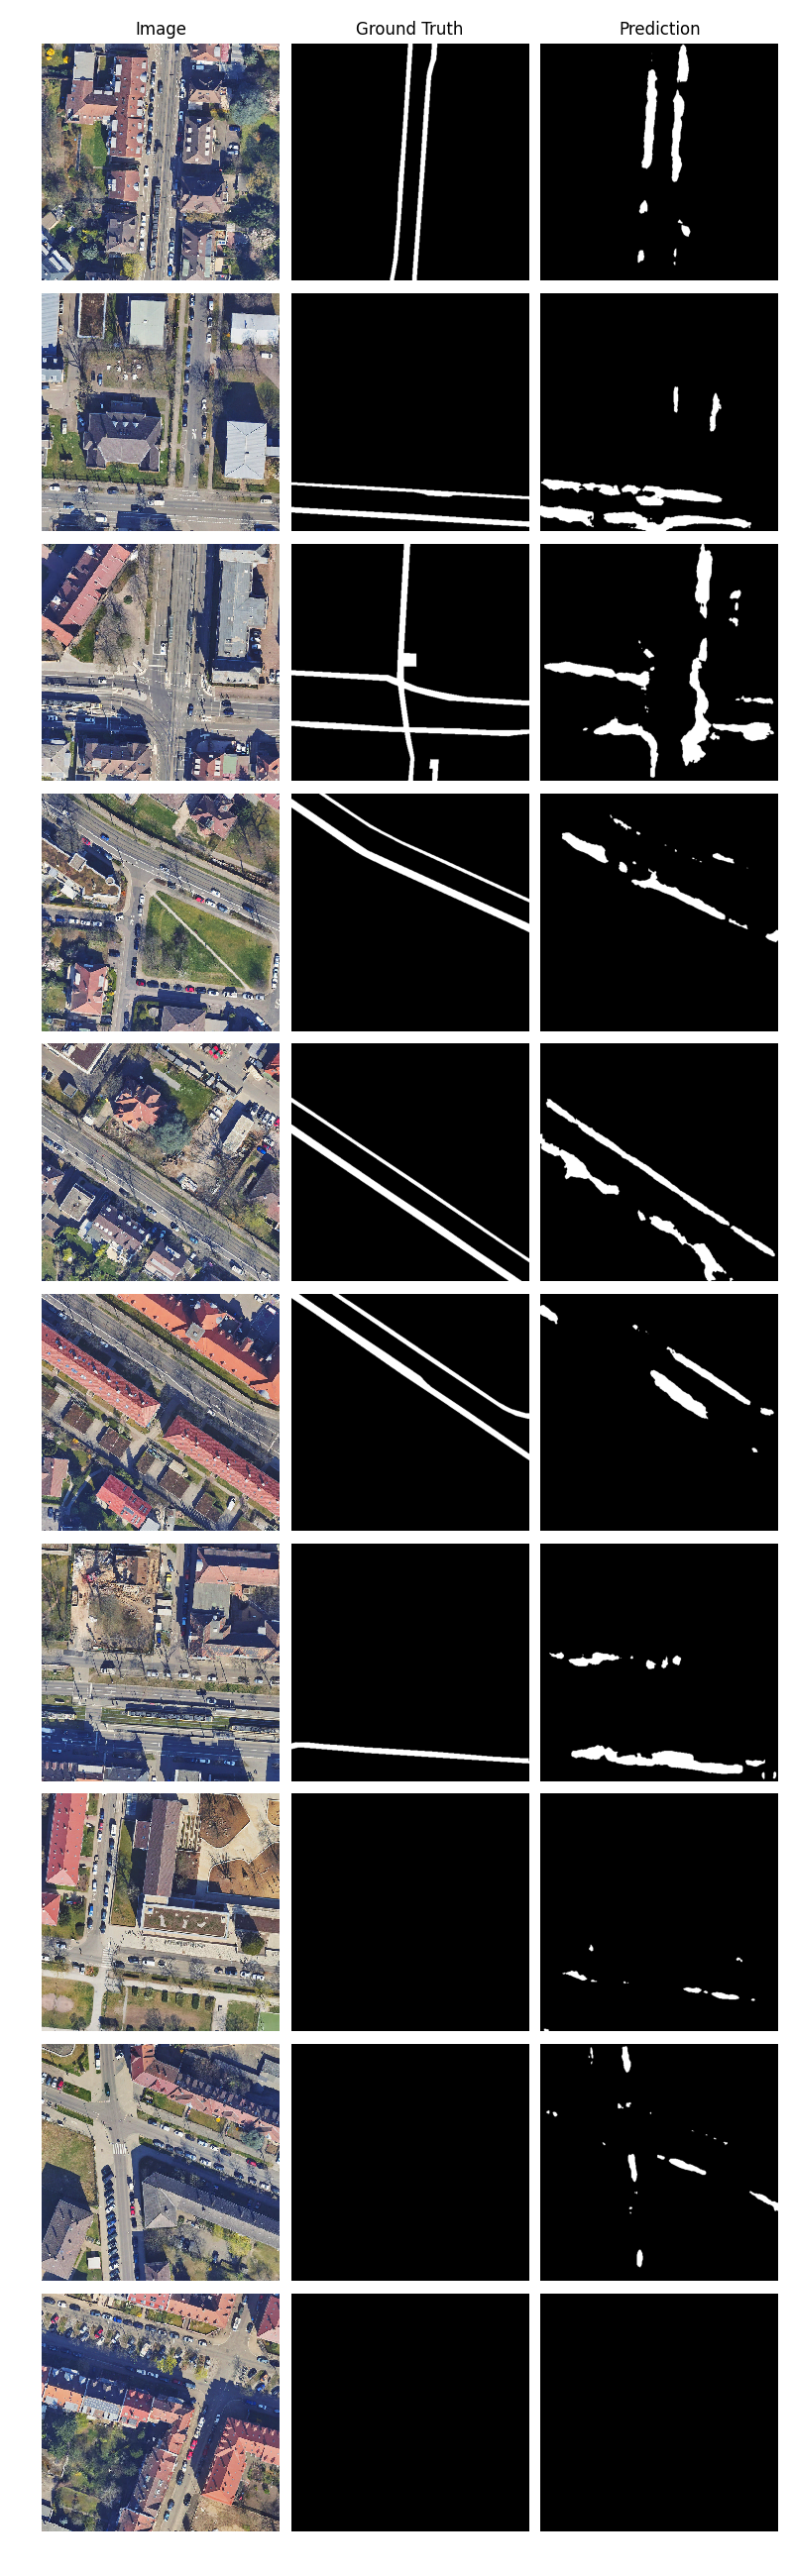
\includegraphics[width=1.\linewidth]{Bilder/Samples-KA/rbunet-s.png}
		\caption{}
	\end{subfigure}

	\caption{Beispiel-Predictions des $RBUNet^l$ (a) und $RBUNet^*$ (b) auf dem Karlsruhe-Datensatz trainiert mit \textit{Basic}-Augmentation.}
	\label{fig:ka-samples-rbunet-l-rbunet-s}
\end{figure}


\begin{figure}[h]
	\centering
	\begin{subfigure}{.4\textwidth}
		\centering
		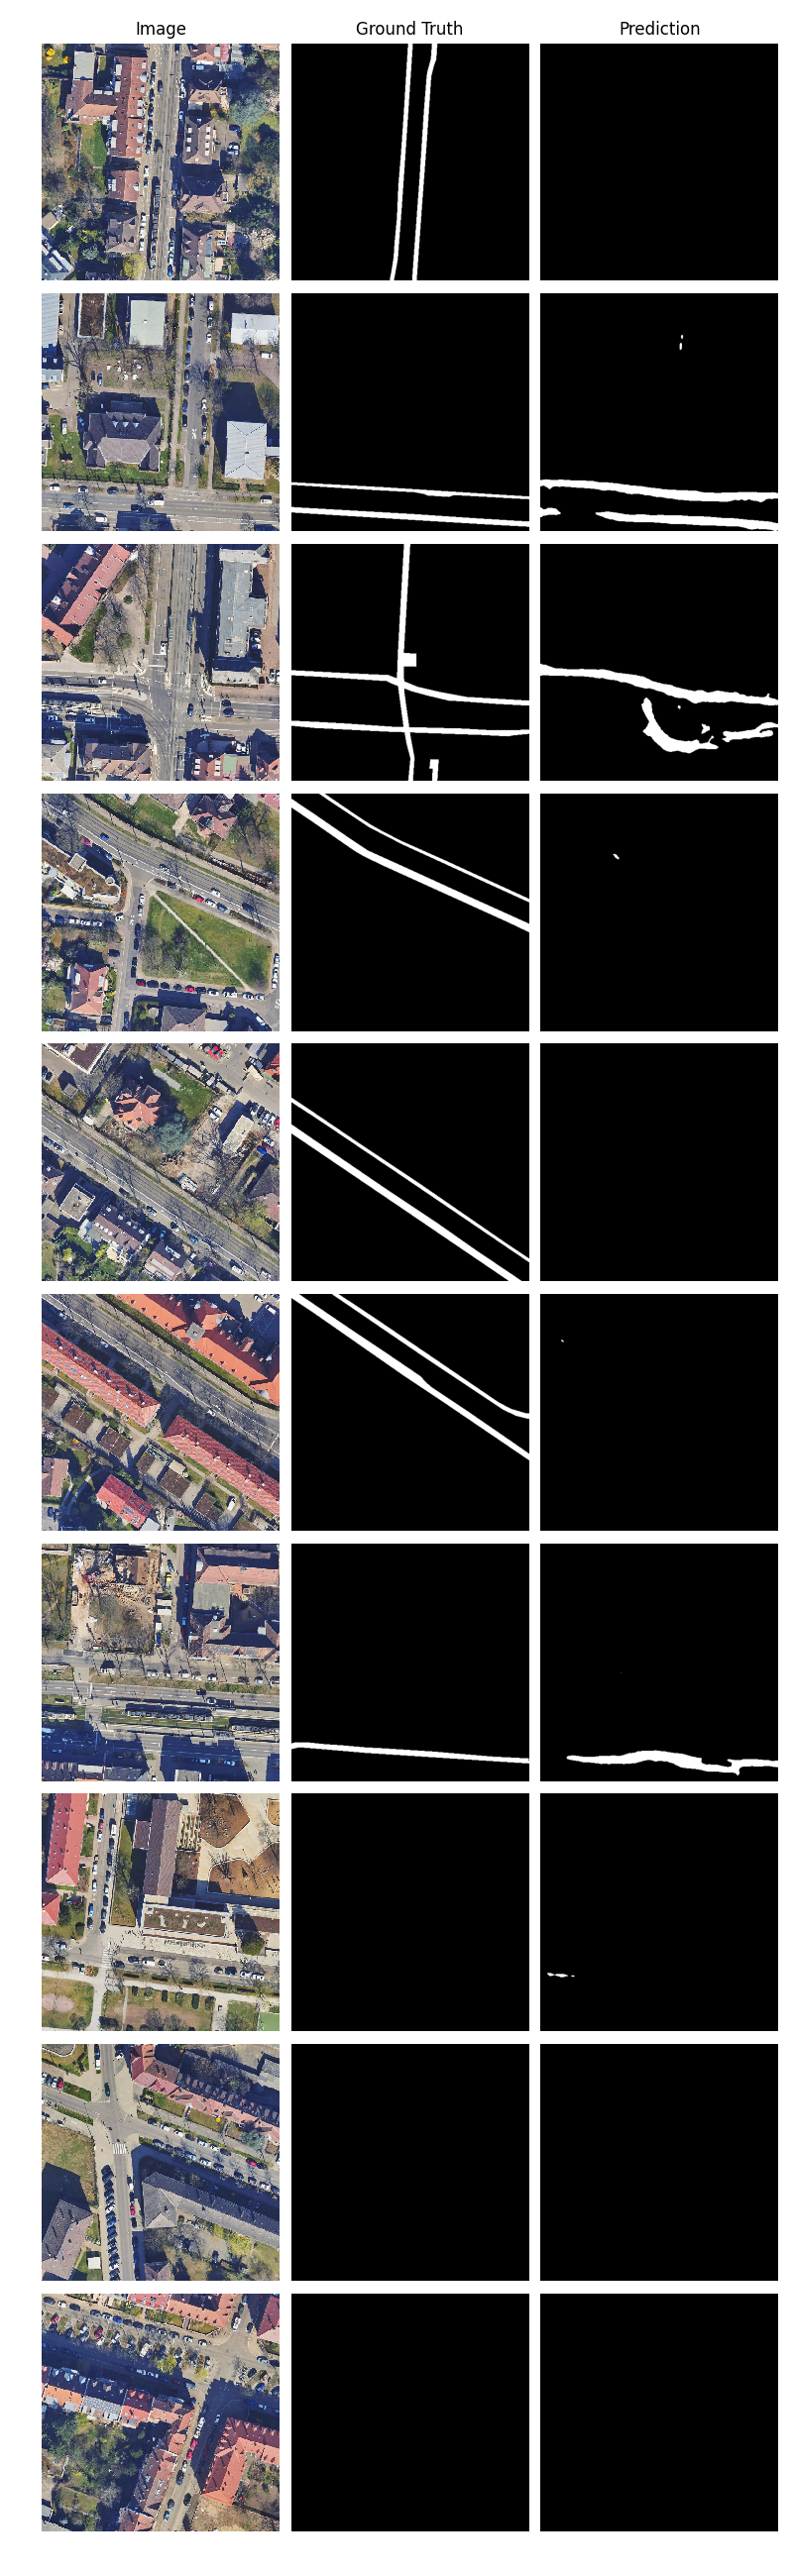
\includegraphics[width=1.\textwidth]{Bilder/karlsruhe-color-samples/rbunet-l.png}
		\caption{}
	\end{subfigure}
	\begin{subfigure}{.4\textwidth}
		\centering
		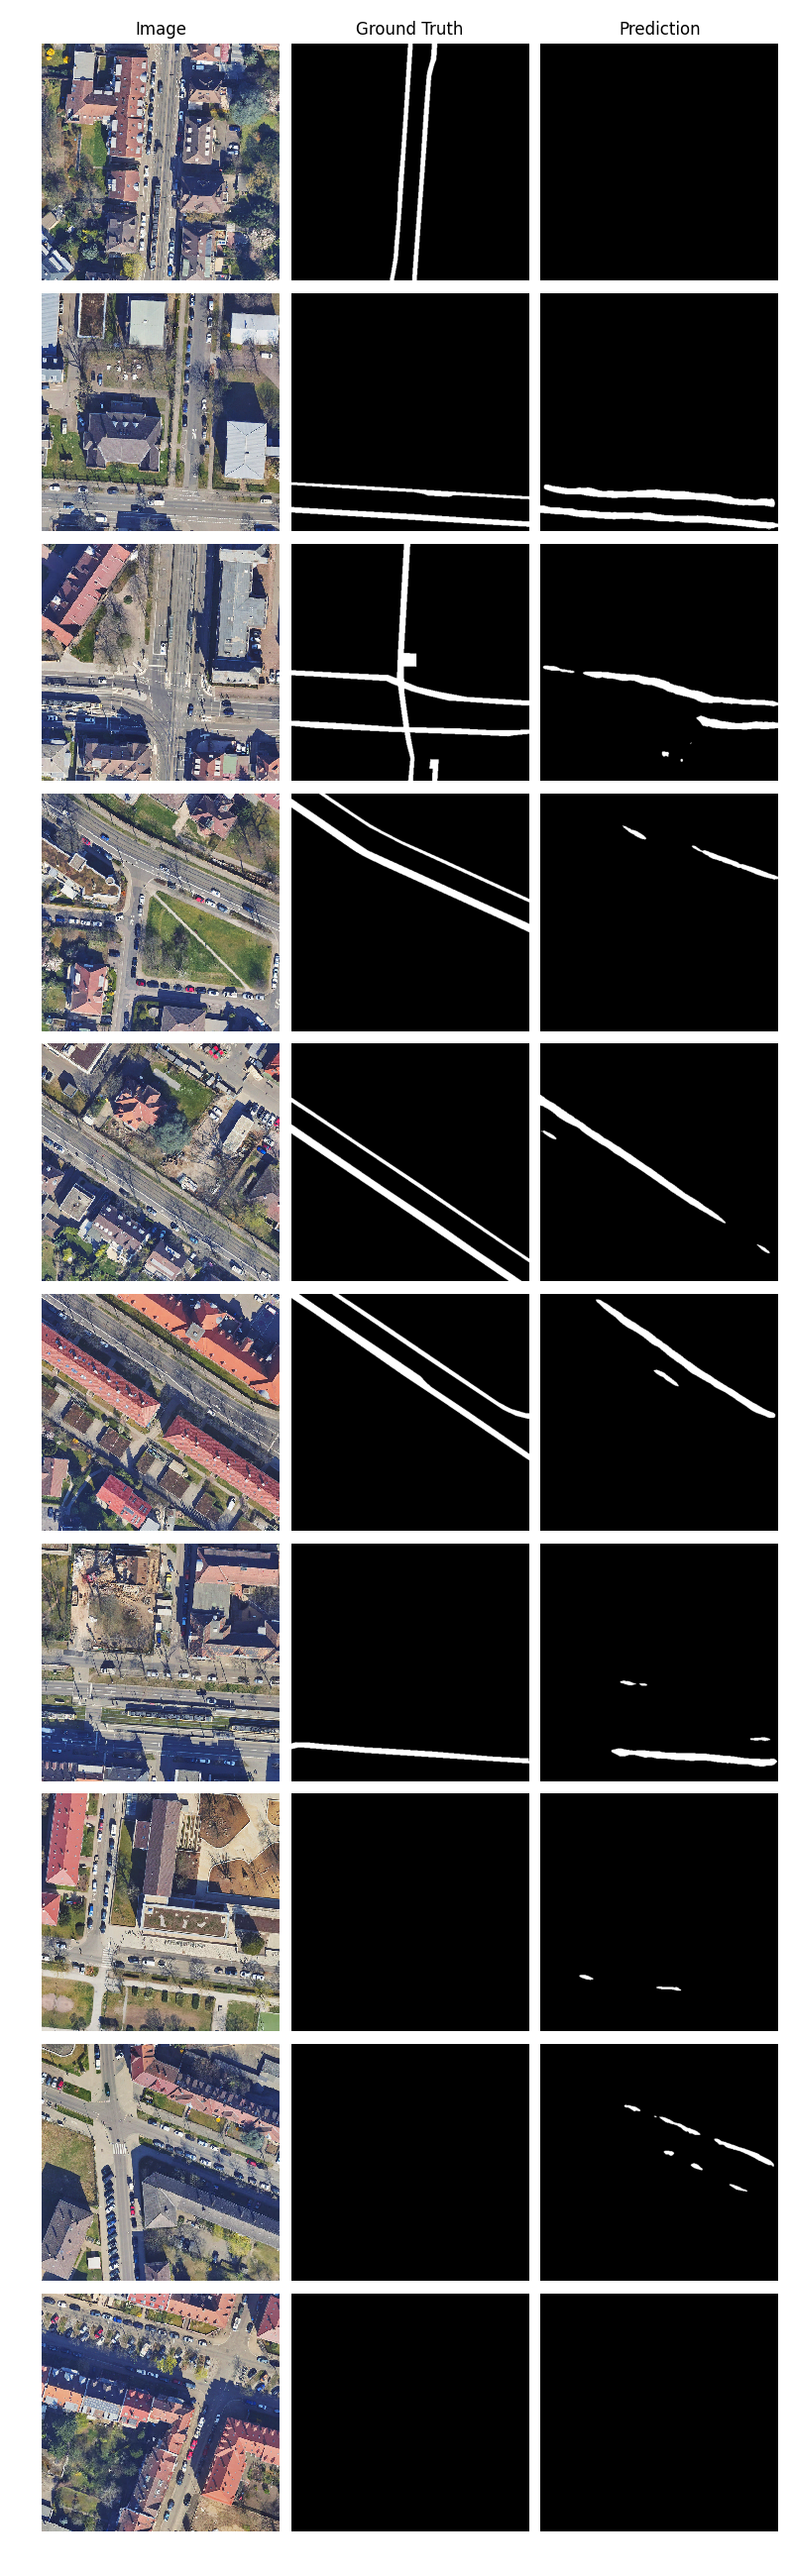
\includegraphics[width=1.\textwidth]{Bilder/karlsruhe-color-samples/rbunet-s.png}
		\caption{}
	\end{subfigure}
	\caption{Beispiel-Predictions des $RBUNet^l$ (a) und $RBUNet^*$ (b) auf dem Karlsruhe-Datensatz trainiert mit \textit{Color}-Augmentation.}
	\label{fig:ka-samples-rbunet-l-rbunet-s-color}
\end{figure}


\begin{figure}[h]
	\centering
	\begin{subfigure}{.4\textwidth}
		\centering
		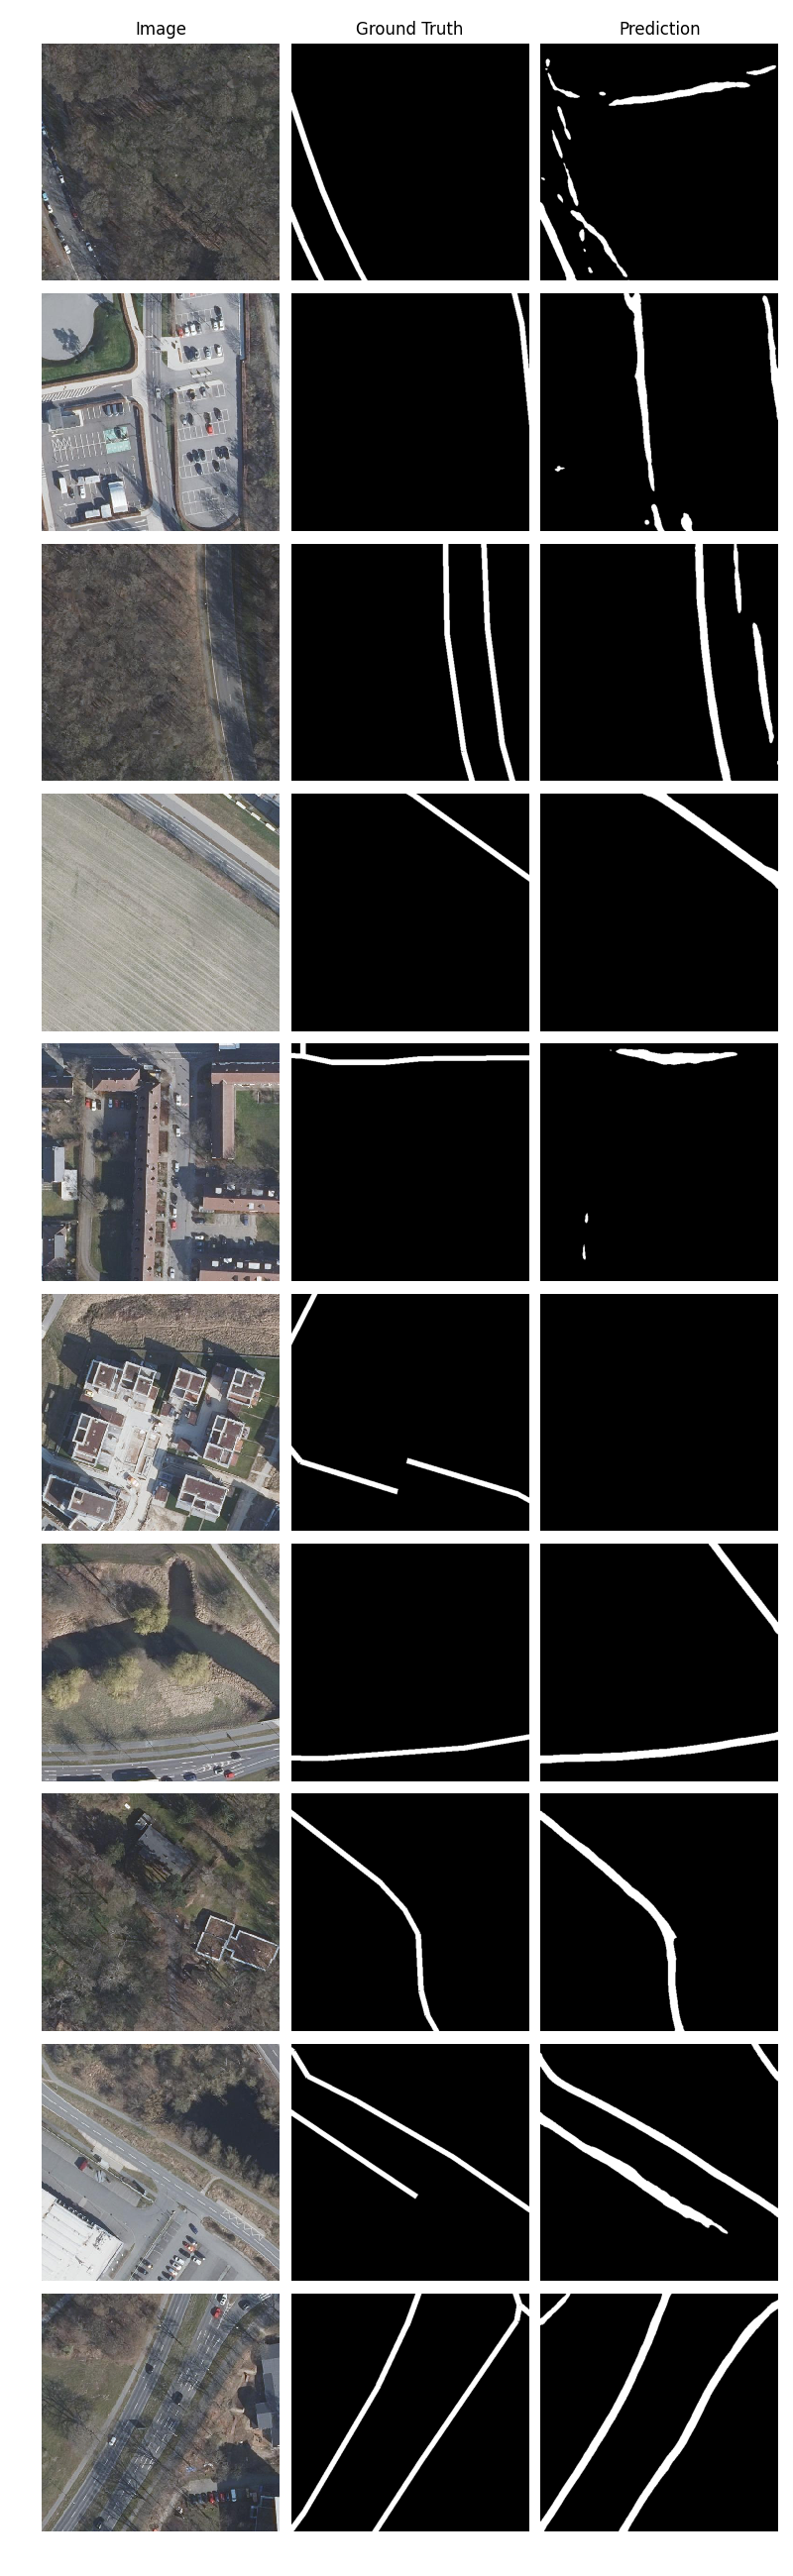
\includegraphics[width=1.\textwidth]{Bilder/wolfsburg-color-samples/rbunet-l.png}
		\caption{}
	\end{subfigure}
	\begin{subfigure}{.4\textwidth}
		\centering
		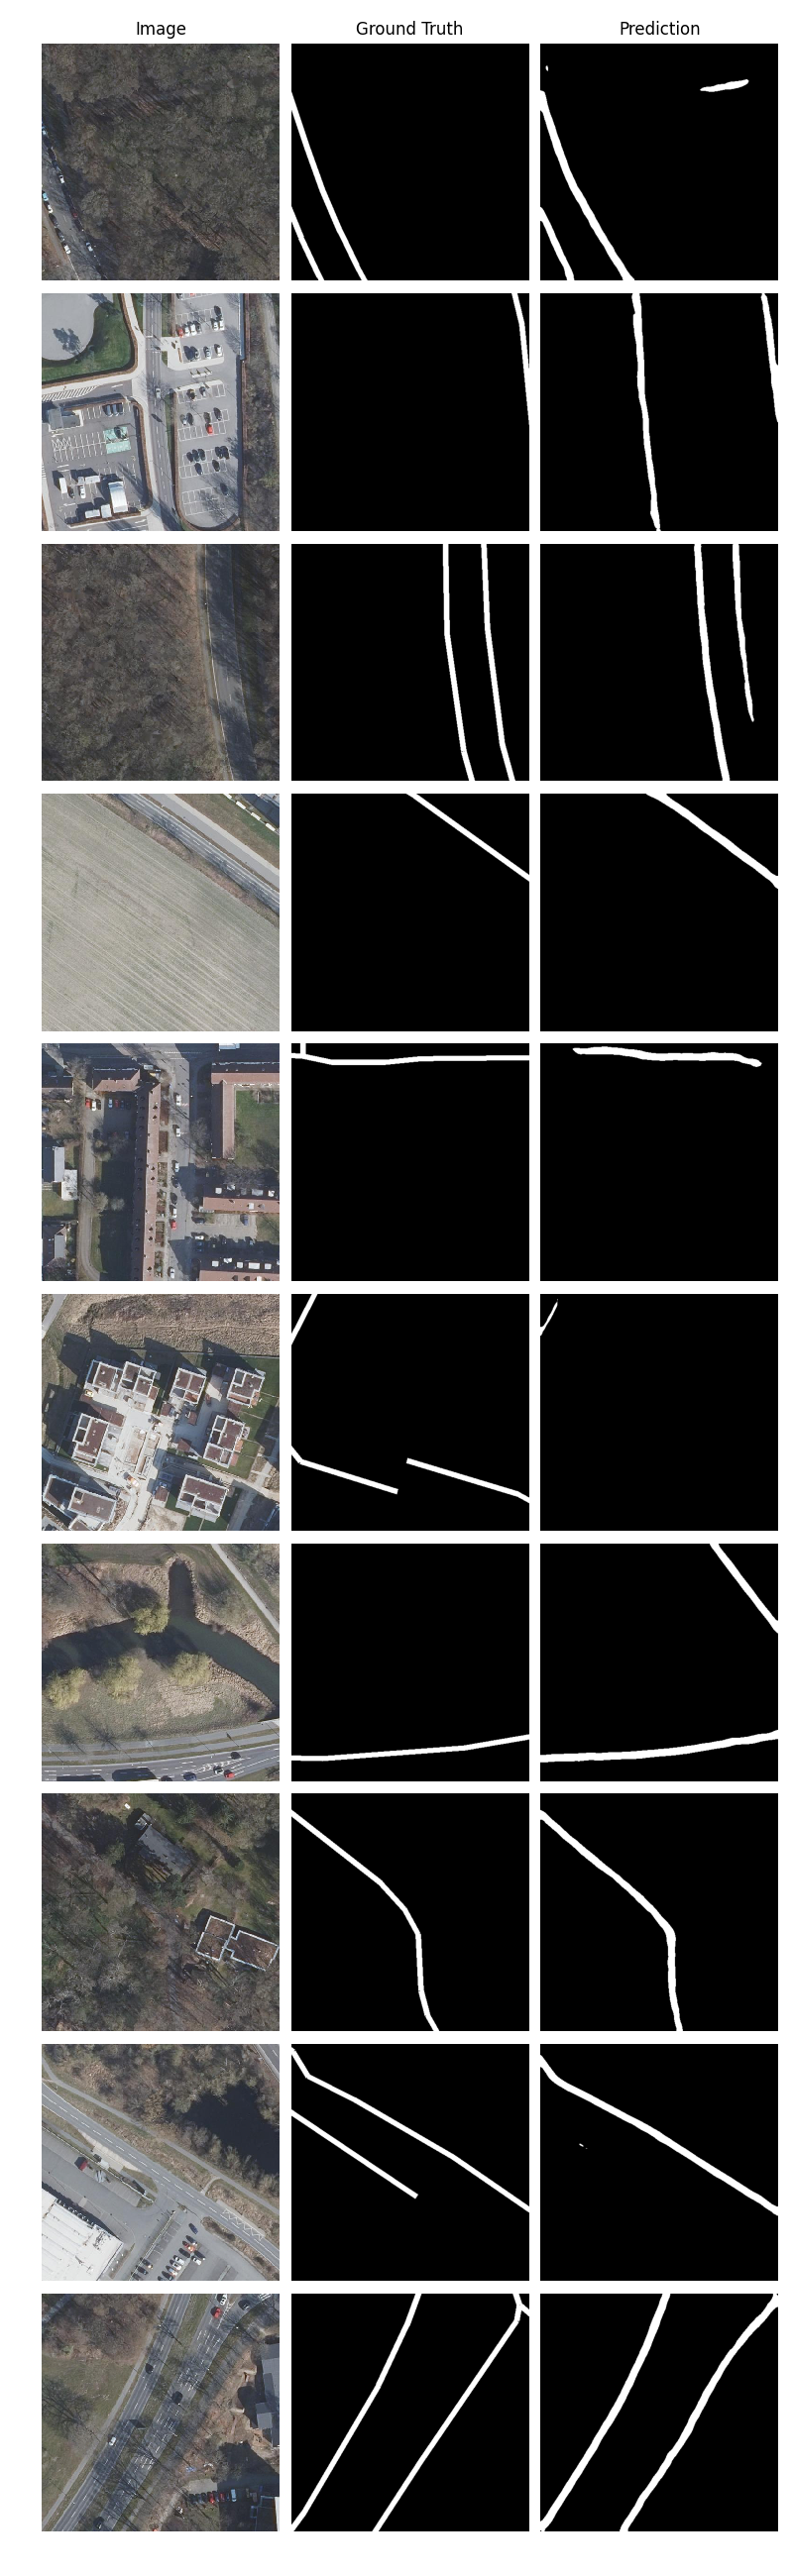
\includegraphics[width=1.\textwidth]{Bilder/wolfsburg-color-samples/rbunet-s.png}
		\caption{}
	\end{subfigure}
	\caption{Beispiel-Predictions des $RBUNet^l$ (a) und $RBUNet^*$ (b) auf dem Wolfsburg-Datensatz trainiert mit \textit{Color}-Augmentation.}
	\label{fig:wolfsburg-samples-rbunet-l-rbunet-s-color}
\end{figure}


\subsection{Ergebnisse auf gefiltertem Karlsruhe-Datensatz}

\begin{table}[ht]
	\centering
	\begin{tabular}{l|cc|cc}
		& \multicolumn{2}{c|}{Basic Aug.} & \multicolumn{2}{c}{Color Aug.} \\ 
		Modell & \ac{IoU} & \ac{BIoU}  & \ac{IoU} & \ac{BIoU}  \\
		\midrule
        BUNet2$^*$ & 02,78 & 07,31  &  14,19 & 27,43 \\
        BUNet2$^l$ & 04,23 & 09,90  &  15,15 & 29,35 \\
        BUNet2$^r$ & 01,94 & 04,67  &  10,45 & 21,33 \\
		\midrule

        BUNet15$^*$ & 07,85 & 17,12  &  16,72 & 37,16 \\
        BUNet15$^l$ & 05,59 & 10,17  &  19,11 & 42,00 \\
        BUNet15$^r$ & 04,94 & 10,06  &  16,41 & 33,52 \\
		\midrule

        VBUNet$^*$ & \underline{\textbf{23,80}} & \underline{\textbf{50,45}} &  \underline{\textbf{22,44}} & \underline{\textbf{47,20}} \\
        VBUNet$^l$ & 11,34 & 22,89 &  07,65 & 18,50 \\
        VBUNet$^r$ & \textbf{22,93} & 38,69 &  20,99 & 39,28 \\
		\midrule

        RBUNet$^*$ & \textbf{20,97} & \textbf{48,42} &  \textbf{21,12} & \textbf{46,11} \\
        RBUNet$^l$ & 04,62 & 08,19 &  18,76 & 34,47 \\
        RBUNet$^r$ & 11,58 & 20,49 &  14,93 & 27,59 \\
		\midrule

        DBUNet$^*$ & 17,52 & \textbf{43,53} &  20,82 & \textbf{45,16} \\
        DBUNet$^l$ & 09,73 & 25,43 &  18,74 & 32,97 \\
        DBUNet$^r$ & 19,77 & 36,33 &  \textbf{22,14} & 44,96 \\
        
	\end{tabular}
	\caption{Ergebnisse der Modelle auf dem Karlsruhe-Datensatz, wobei Bilder mit leeren Masken entfernt wurden. 
    In Prozent.}
	\label{tab:results-ka-small}
\end{table}

\autoref{tab:results-ka-small} zeigt die Test-Ergebnisse der Modelle aus \autoref{tab:results} 
auf allen 49 $512{\times}512$-Ausschnitten des Karlsruhe-Datensatz (s. \autoref{sec:karlsruhe}), 
\textit{die Radwegen enthalten}, in Prozent. 
Ein Ausschnitt enthält einen Radweg, wenn in der zugehörigen Label-Maske mindestens ein Pixel als Radweg annotiert ist. \\
Pro Spalte sind die höchsten drei Ergebnisse hervorgehoben und das höchste unterstrichen.
Die \ac{BIoU} hat eine Puffergröße von 15 Pixeln, wie in \autoref{sec:eval:biou} festgelegt.

\subsection{Ergebnisse bei fehlender Annotation}

Wie in \autoref{sec:bike-data} und \ref{sec:karlsruhe} beschrieben, wurde der BikeSat-Datensatz automatisch 
annotiert und der Karlsruhe-Datensatz von Menschen. Die Netze sind mit dem BikeSat-Datensatz trainiert. 
Wie bereits in \autoref{sec:bike-data} erwähnt, erhält die Datengrundlage zum BikeSat-Datensatz 
in einer von Menschen gesichteten und bewerteten Stichprobe \textbf{722} von \textbf{724} realen Radwegen.
Es fehlen also zwei Radwege. 

Die manuell von Menschen annotierten Bilder des Karlsruhe-Datensatzes zeigen dagegen eine höhere 
Fehlerquote. Die bestehenden Label sind zwar genauer platziert, aber dafür weniger vollständig. 
Hier ist bei einer Sichtung der Daten aufgefallen, dass ca. 15\% der Radwege nicht annotiert sind. 
Das hat aber keine Auswirkung auf das Training, da der Karlsruhe-Datensatz nur zum Testen verwendet wird.
\autoref{fig:annotation-mistake} zeigt ausgewählte Predictions (b)-(d) 
zu einem Ausschnitt aus dem Karlsruhe-Datensatz, bei dem bei der manuellen Annotation 
Radwege in der Straße, die von links unten nach rechts oben verläuft, übersehen wurden. 
In den Ausschnitten (c) und (d) sind die Radwege trotzdem erkannt, während es aber auch 
Beispiele wie (b) gibt, worin die querenden Radwege nicht getroffen sind. Ausschnitte (c) 
und (d) zeigen allerdings, dass die Netze Radwege erkennen können, die ein Mensch übersieht.
Es war allerdings kein Netz in der Lage für den gegebenen Bildausschnitt alle Radwege korrekt 
zu erkennen. \\
Was außerdem auffällig ist, ist, dass in Bild (c) der Radweg rechts unten genau getroffen ist 
(vgl. menschliche Annotation aus (a)), während in Bild (c) und (d) der Gehweg neben dem eigentlichen 
Radweg annotiert ist. Zudem fällt in (d) ein grober Fehler des Netzes auf, da hier klar Teile des 
blauen Dachs auf der rechten Bildseite annotiert sind.

\begin{figure}
	\centering
	\begin{subfigure}{.45\textwidth}
		\centering
		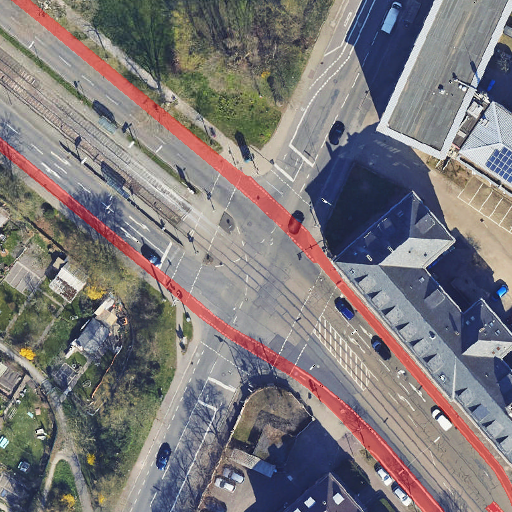
\includegraphics[width=1.\linewidth]{Bilder/annotation-mistake/overlayed.png}
		\caption{}
	\end{subfigure}
	\begin{subfigure}{.45\textwidth}
		\centering
		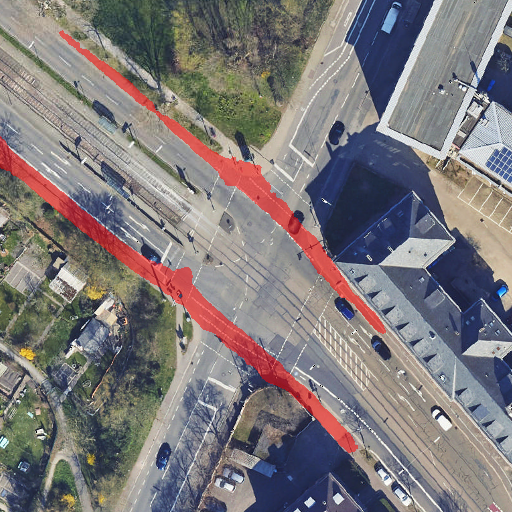
\includegraphics[width=1.\linewidth]{Bilder/annotation-mistake/straight-dbunet-r.png}
		\caption{}
	\end{subfigure} 
	\begin{subfigure}{.45\textwidth}
		\centering
		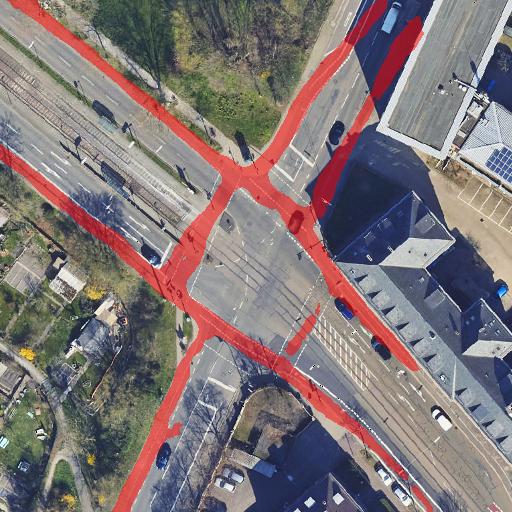
\includegraphics[width=1.\linewidth]{Bilder/annotation-mistake/fitting-vbunet-r.png}
		\caption{}
	\end{subfigure}
	\begin{subfigure}{.45\textwidth}
		\centering
		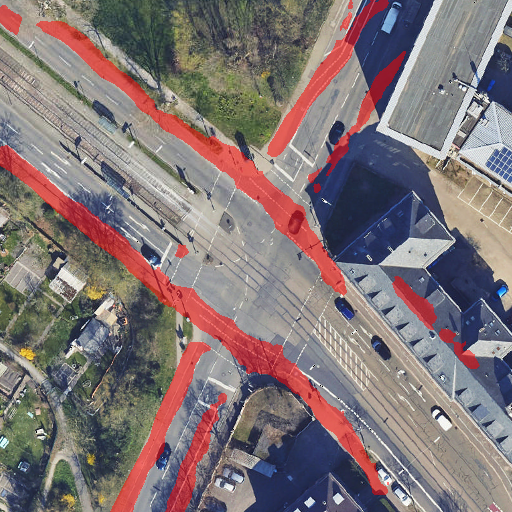
\includegraphics[width=1.\linewidth]{Bilder/annotation-mistake/full-vbunet-s.png}
		\caption{}
	\end{subfigure}

	\caption{(a) zeigt ein manuell annotierten Ausschnitt aus dem Karlsruhe-Datensatz, wobei Radwege 
	fälschlicherweise nicht annotiert sind. Abbildungen (b), (c) und (d) zeigen die Predictions von \ac{DBUNet}$^r$,
	\ac{VBUNet}$^r$, bzw. \ac{VBUNet}$^*$.}
	\label{fig:annotation-mistake}
\end{figure}

% networks tested with karlsruhe test data set  

% testing ./../Models/Double-Data\backbones\bike_mapper_pre-train-scratch-densenet121_Aug_IoU3076_q6178.h5
% iou: 0.07135618478059769, quality:0.45967867970466614

% testing ./../Models/Double-Data\backbones\bike_mapper_pre-train-scratch-resnet34_Aug_IoU2911_q6053.h5
% iou: 0.11737822741270065, quality:0.3280484974384308

% testing ./../Models/Double-Data\backbones\bike_mapper_pre-train-scratch-vgg16_Aug_IoU3045_q6148.h5
% iou: 0.09694375097751617, quality:0.3783626854419708

% testing ./../Models/Double-Data\pre-train\bike_mapper_pre-train-freeze-left_Aug_IoU2448_q5177.h5
% iou: 0.020918812602758408, quality:0.1211065948009491

% testing ./../Models/Double-Data\pre-train\bike_mapper_pre-train-freeze-right_Aug_IoU2535_q5127.h5
% iou: 0.09364935010671616, quality:0.47571051120758057

% testing ./../Models/Double-Data\pre-train\bike_mapper_triple-param_pre-train-freeze-left_Aug_IoU2814_q5714.h5
% iou: 0.1647404581308365, quality:0.5417148470878601

% testing ./../Models/Double-Data\pre-train\bike_mapper_triple-param_pre-train-freeze-right_Aug_IoU2822_q5726.h5
% iou: 0.10167630761861801, quality:0.5381019115447998

% testing ./../Models/Double-Data\road-pre-trained-backbones\bike_mapper_pre-train-densenet121freeze-left_Aug_IoU3155_q6238.h5
% iou: 0.17469285428524017, quality:0.5520145893096924

% testing ./../Models/Double-Data\road-pre-trained-backbones\bike_mapper_pre-train-densenet121freeze-right_Aug_IoU3212_q6299.h5
% iou: 0.14031212031841278, quality:0.5172706246376038

% testing ./../Models/Double-Data\road-pre-trained-backbones\bike_mapper_pre-train-resnet34freeze-left_Aug_IoU3098_q6051.h5
% iou: 0.24674279987812042, quality:0.6527144312858582

% testing ./../Models/Double-Data\road-pre-trained-backbones\bike_mapper_pre-train-resnet34freeze-right_Aug_IoU3131_q6355.h5
% iou: 0.18207795917987823, quality:0.5552724599838257

% testing ./../Models/Double-Data\road-pre-trained-backbones\bike_mapper_pre-train-vgg16freeze-left_Aug_IoU3224_q6293.h5
% iou: 0.12852726876735687, quality:0.5490880012512207

% testing ./../Models/Double-Data\road-pre-trained-backbones\bike_mapper_pre-train-vgg16freeze-right_Aug_IoU3184_q6151.h5
% iou: 0.175296351313591, quality:0.6151095628738403

% testing ./../Models/Double-Data\bike_mapper_scratch_Aug_IoU2354_q4771.h5
% iou: 0.013092363253235817, quality:0.3479517698287964

% testing ./../Models/Double-Data\bike_mapper_scratch_triple-param_Aug_IoU2793_q5655.h5
% iou: 0.21523651480674744, quality:0.5924956798553467


\chapter{Diskussion}

Im Folgenden werden die zuvor präsentierten Ergebnisse diskutiert. Zunächst werden die beobachteten Phänomene 
bei der Straßenerkennung betrachtet und daraufhin die bei der Radwegerkennung.

\section{Straßenerkennung}

Die Ergebnisse der Straßenerkennung können als gut im Vergleich zur Literatur eingeordnet werden. 
Das beste Modell ist hierbei das \ac{VBUNet}, welches mit einer Test-IoU von 64,26\% mit den 
performantesten Modellen aus \autoref{sec:state-of-the-art-roads} mithalten kann. Hier wurden 
Spitzenwerte von 67,10 und 65,60\% auf dem Massachusetts- bzw. Deep-Globe-Datensatz erzielt. 
Die Hyperparameter dieser Modelle sind auf das jeweilige Problem optimiert, während das VBUNet nicht optimiert ist. 
Dafür sind die Ergebnisse sehr gut. \\  
Was überraschend ist, ist, dass im Pre-Training in dieser Arbeit 
das VBUNet die besten Ergebnisse erzielt, während in der Literatur die besten Modelle ResNet-Derivate sind. 
Das kann daran liegen, dass in der Literatur die Modelle isoliert auf dem Massachusetts- und Deep-Globe-Datensatz 
trainiert werden. In dieser Arbeit sind alle Netze hingegen auf der Vereinigung der beiden Datensätze trainiert. 
Die beiden Datensätze stellen allerdings sehr unterschiedliche Landschaften dar. 
Möglicherweise funktioniert also ResNet, welches eine viel höhere Komplexität als VGG aufweist, besser 
als Spezialisierung auf einer der beiden Landschaften, ist also besonders angepasst auf die jeweilige Landschaft, 
während VGG mit der geringeren Komplexität besser Straßen generalisieren kann und deshalb robuster ist. 
Eine weitere, simplere Erklärung ist, dass in dieser Arbeit die Netze lediglich mit einem Satz 
an Hyperparametern und einem festen Seed genau ein mal trainiert sind. Außerdem sind die Ergebnisse 
nicht mit einer Kreuzvalidierung überprüft.
Es kann also lediglich eine schlechte Besetzung der Hyperparameter und Startwerte für das ResNet und eine 
gute für VGG vorliegen. \\
Der Erwartung entsprechend kann BUNet2 mit der eher geringen Parameteranzahl von 2 Mio. Parametern nicht 
mit der Leistung der restlichen Netze konkurrieren. BUNet15 zeigt, dass BUNet2 schlicht eine zu geringe 
Komplexität aufweist, um die Straßen so gut wie die komplexeren Netze segmentieren zu können. 
Trotzdem ist die Leistung nicht schlecht. Mit nur einem Bruchteil der Parameter der übrigen Netze
kann BUNet2 zumindest vergleichbare Ergebnisse erzeugen. \\
Während BUNet15 und BUNet2 bis auf die Parameteranzahl identisch sind, weswegen sich ein Unterschied in der 
Performance auf den Komplexitätsunterschied zurückführen lässt, ist bei dem Performance-Unterschied 
zwischen BUNet15 und den Backbone-Architekturen, insbesondere RBUNet und DBUNet, unklar, ob die kleine 
Differenz von wenigen Prozenten in der IoU bzw. der BIoU in der unterschiedlichen Architektur oder dem 
Pre-Training der Backbone-Architekturen auf ImageNet begründet ist. Eventuell ist RBUNet z.B. die schlechtere 
Architektur, erzielt aber bessere Ergebnisse als BUNet15 aufgrund des Pre-Trainings auf ImageNet. 
Ob das der Fall ist, kann nur durch weitere Experimente geklärt werden, die BUNet15 mit den nicht vortrainierten 
Backbone-Netzen vergleicht. In jedem Fall scheint aber das Pre-Training auf ImageNet nur geringe 
Performance-Verbesserungen herbeizuführen. 

\subsection{BIoU für die Straßenerkennung}

\begin{wrapfigure}{r}{0.40\textwidth}
	\centering
	\vspace{-20pt} % Manchmal möchte man den oberen Abstand selbst anpassen
	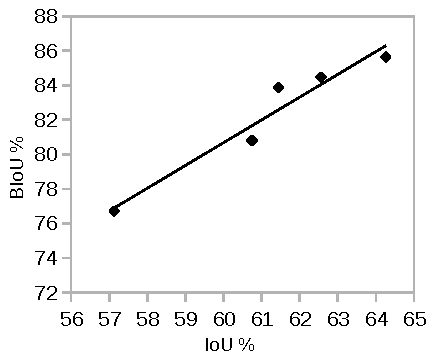
\includegraphics[width=0.35\textwidth]{Bilder/iou-biou-correlation.pdf}
	\vspace{-5pt}
	% Das folgende ist ein Trick, um "Abbilgung x.y" in eine
	% eigene Zeile zu packen. Der Text zwischen [ und ] steht
	% im Abbildungsverzeichnis. Der Text darunter wird
	% tatsächlich angezeigt.
	\caption[BIoU der Modelle der Straßenerkennung aufgetragen über deren IoU.]{\unskip}
	BIoU über IoU in Prozent (Straßenerkennung). Pos. Korrelation mit $r = 0,9707$. 
	\label{fig:iou-biou-corr}
	% \vspace{-20pt}
\end{wrapfigure}

Im Gegensatz zu den Radweg-Datensätzen bei der Maskenerstellung des Straßendatensatzes keinerlei Schätzung 
über die Lage der Wege eingesetzt worden. Die Masken sind also überwiegend deckungsgleich mit den tatsächlichen 
Straßen im Input-Bild, während bei den Radwegen manche Radwege grob versetzt positioniert sind. 
Deswegen muss die BIoU bei der Straßenerkennung keine komplette Verschiebung der Prediction zur Ground-Truth ausgleichen, 
sondern glättet lediglich die IoU im Randbereich der Straßen. Daher ist die Straßenerkennung geeignet, 
um zu untersuchen, ob die BIoU erwartungsgemäß arbeitet. \autoref{fig:iou-biou-corr} zeigt die Testergebnisse der 
Straßenerkennung mit der BIoU in Prozent aufgetragen über der IoU in Prozent für die jeweiligen Modelle. 
Es herrscht eine starke positive Korrelation zwischen der IoU und BIoU mit Korrelationskoeffizient $r = 0,9707$. 
Die starke Korrelation spricht für die vorangegangene Annahme, dass im Falle der Straßendetektion die BIoU 
ungerade Predictions glättet und fairer bewertet, bzw. näher an dem ist, wie ein Mensch die Performanz der 
Netze wahrnimmt. Die sehr streng bewertende IoU gibt einen schlechten Eindruck von der Leistungsfähigkeit des Netzes. 
Aus den Beispielpredictions der Straßenerkennung erhält ein menschlicher Beobachter nicht den Eindruck, 
dass nur circa 60\% der Straßen richtig erkannt worden sind, sondern eher im Bereich von 80\% oder mehr. 
Damit beweist sich die BIoU, als ein Maß, welches im Falle der Straßenerkennung lediglich die IoU so anhebt, 
dass eine zu schmal oder zu breit gezeichnete Predicition mit rauen Kanten als (qualitativ) korrekt in 
die Bewertung einfließt.  

\section{Radwegerkennung}

Die Ergebnisse für die Radwegerkennung (vgl. \autoref{tab:results}) zeigen, dass die Ergebnisse der 
Radwegerkennung statistisch signifikant\footnote{
	$p = 1,887\cdot 10^{-8}$ für IoU und $p = 3,77\cdot 10^{-7}$ für BIoU
	des einseitigen Zweistichproben-Welch-Test zwischen der Straßenerkennung 
	und der Radwegerkennung für Basic-Aug. 
} schlechter sind, als die der Straßenerkennung. Hierfür gibt es folgende Gründe:
\begin{enumerate}
	\item Das Problem der Radwegerkennung ist schwerer. Für die Radwegerkennung fällt es selbst Menschen schwer 
	diese auf Satellitenbildern zu erkennen. Für Fahrradstreifen am Straßenrand ist das noch gut möglich, 
	aber für oft überdeckte und überschattete Fahrradwege neben der Straße, die zum Beispiel durch einen Grünstreifen 
	von der Straße getrennt sind und mit dem Fußweg verbunden sind, ist schwierig festzustellen, ob ein Radweg 
	vorhanden ist, oder ob es sich nur um einen Gehweg handelt. Außerdem weisen Radwege weitaus 
	heterogenere Beläge auf, als städtische Straßen. Für Radwege kommen Asphalt, unterschiedlich farbene Pflastersteine,
	Schotter, rot oder grün gefärbter Asphalt und andere Untergründe zum Einsatz, 
	während die allermeisten Straßen in der Stadt aus Asphalt bestehen.
	Weiterhin gibt es viel weniger Radwege als Straßen, wodurch in den Trainingsdaten eine große Imabalance 
	und generell weniger Beispiele vorhanden sind, als in einem ähnlich großen Datensatz für die Straßenerkennung. 
	Auch unterscheiden sich Radwege zwischen Ländern und selbst Städten eines Landes weitaus stärker, als Straßen.
	\item Die automatisch generierten Annotationen sind überwiegend (ca. zu 83\%; vgl. \autoref{sec:quality-of-masks})
	auf dem Niveau einer Annotation durch Menschen, allerdings könnte der Anteil der Annotationen, die schlichtweg
	falsch sind, die Ergebnisse stark beeinträchtigen. Um diese Hypothese zu verifizieren sind weitere 
	Experimente mit einem besser annotierten Datensatz notwendig. Ein durch Menschen annotierter Datensatz 
	muss dafür klar definieren, was die Labelnden als Radweg anerkennen, da bei Radwegen auf Luftbildern 
	nicht unbedingt ein allgemeiner Konsens besteht, was als Radweg zu markieren zählt. Durch menschliche Annotation 
	kann aber zumindest ausgeschlossen werden, dass Pixel als Radweg annotiert sind, die eine Wiese oder ein Gebäude zeigen.
	\item Möglicherweise ist die semantische Segmentierung zum Erkennen der Radwege eine zu detaillierte Methode. 
	Um die Forschungsfrage dieser Arbeit -- existiert ein Radweg an dieser Straße und wenn ja, in welche Richtung -- 
	zu beantworten, ist die semantische Segmentierung der Radwege übermäßig. Die semantische Segmentierung 
	schafft mehr Informationen, als benötigt werden. Das bietet zwar auch Vorteile, dass zum Beispiel der Radweg 
	auf einem Luftbild als solcher eingefärbt werden kann, aber verlangt auch weitaus genauere Annotationen. \\
	Eine Alternative Herangehensweise kann sein, das Problem so zu modellieren, dass die Modelle direkt einen Graphen
	an Radwegen extrahieren, anstatt zuerst die zum Radweg gehörigen Pixel zu annotieren und die Graphenextraktion 
	in einem externen Schritt vorzunehmen. Dabei können als Label direkt die Graphen aus \ac{OSM} verwendet werden 
	und die Rad\textit{streifen} müssen nicht verschoben werden. Das Problem hierbei ist, zu Kodieren, ob 
	ein Radweg rechtsseitig oder linksseitig vorliegt, da die Definition von rechts- und linksseitig abhängt  
	von dem von \ac{OSM} willkürlich gewählten Verlauf der Straße. Hierfür könnte der Begriff von links- und 
	rechtsseitig transformiert werden in östlich und nördlich, bzw. in westlich und südlich von der Straße.    
\end{enumerate}
Obwohl die Radwegerkennung nicht so gute Ergebnisse liefert, wie die Straßenerkennung, und die Ergebnisse 
für die Radwegerkennung durchaus Verbesserungspotential bieten, lässt sich aus der Arbeit 
schließen, dass es möglich ist, andere Strukturen der städtischen Infrastruktur aus Luftbildern zu erkennen, 
als Straßen. 

\subsection{Ergebnisse auf Karlsruhe gegenüber BikeSat und Wolfsburg}

Aus allen Experimenten geht hervor, dass die Performance auf dem (ungefilterten und gefilterten) Karlsruhe-Datensatz deutlich schlechter ist, 
als auf dem BikeSat- und Wolfsburg-Datensatz. Außerdem hat die Color-Aug. keine Verbesserung gegenüber 
Basic-Aug. hervorgerufen. Auch ist der Wolfsburg-Datensatz, der eine andere Stadt, bei gleicher Optik der Bilder, 
zeigt, als der BikeSat-Datensatz, gleich auf mit dem BikeSat-Datensatz. Wolfsburg weist aber eine sehr ähnliche 
Infrastruktur zu den anderen Städten aus Niedersachsen (BikeSat) auf. Daraus lässt sich schließen, 
dass für die schlechte Performance auf dem Karlsruhe-Datensatz wahrscheinlich nicht die Optik der Bilder verantwortlich 
ist, sondern die sehr unterschiedliche Infrastruktur der Fahrradwege oder das allgemeine Stadtbild. 
So hat Karlsruhe beispielsweise deutlich mehr Fahrradstreifen am Straßenrand als die niedersächsischen Städte. 
Diese Beobachtung beantwortet die Forschungsfrage, ob Ergebnisse auf Städten unterschiedlicher Infrastrukturen 
übertragbar sind. So ist eine Übertragung bedingt möglich, aber es liegt nahe, dass mit Performance-Einbußen zu rechnen ist, 
die die Stärke des Unterschieds der Infrastrukturen widerspiegeln. 
Um diese These zu belegen, bedarf es jedoch weiterer Experimente mit mehr Städten. Eventuell ist dann 
auch eine Proportionalität zwischen Performance-Einbußen auf für das Modell unbekannten Städten und der Stärke 
des Unterschieds der Städte erkennbar. Insofern eine Quantifizierung des Unterschieds der Städte gelingt. 

Die signifikant bessere BIoU von Wolfsburg im Gegensatz zu BikeSat wird darauf zurückgeführt, dass 
Wolfsburg eine sehr ähnliche Fahrrad-Infrastruktur aufweist, wie der BikeSat-Datensatz, aber weniger 
Samples beinhaltet, die schwierig als Radweg zu erkennen sind. Außerdem ist der Unterschied nur gering, 
da der Unterschied in IoU keine statistische Signifikanz erreicht. 

% schlechtere Ergebnisse als Straßenkennung, was probleme ? 
% warum karslrueh so viel schlechterbiou
% warum wolfsburg besser ? 
% Wolfsburg doch eher ungeeignet weil zu ähnlich 
% experimente mit anderen städten
% color augmentation nicht viel grebracht -> liegt wohl an stadtbild
% netze eher konservativ wie karlsrueh prediction zeigt
% warum gefilterter schlechter?

effizienz des pretraining 
warum wenig unterschiede zwischen den netzen

\subsection{Effektivität des Fine-Tunings}



\subsection{BIoU für Radwegerkennung}

\subsection{Gefilterter Straßendatensatz}

\newcommand{\overbar}[1]{\mkern 8mu\overline{\mkern-8mu#1\mkern-8mu}\mkern 8mu}

Sei $K_{fil} \subset K_{unfil}$ mit $|K_{fil}| = 49; ~|K_{unfil}| = 196$ der gefilterte Kalrsruhe-Datensatz 
als Teilmenge vom ungefilterten Karlsruhe-Datensatz $K_{unfil}$. Wobei gefiltert bedeutet, dass 
keine leere Ground-Truth-Maske existiert, alle Bilder also einen Radweg enthalten.
Die Ergebnisse aus \autoref{tab:results} und \autoref{tab:results-ka-small} mit der Visualisierung aus 
\autoref{fig:iou-biou-corr-ka} zeigen, dass die BIoU auf dem gefilterten Datensatz $K_{fil}$ signifikant 
schlechter ist, als auf dem ungefilterten. Da die BIoU als aritmethisches Mittel der BIoU-Werte der einzelnen Bilder 
berechnet wird und die Predictions auf den Bildern von $K_{fil} \cap K_{unfil} = K_{fil}$ gleich ausfallen, 
lässt sich aus den durchschnittlichen Ergebnissen den beiden Datensätze die durchschnittliche BIoU auf den leeren Bildern 
$K_{leer} := K_{unfil} \setminus K_{fil};~ |K_{leer}| = |K_{unfil}| - |K_{fil}| = 147$ über   
\begin{align}
	\overbar{BIoU_{K_{unfil}}} = \frac{|K_{fil}| \cdot \overbar{BIoU_{K_{fil}}} + |K_{leer}| \cdot \overbar{BIoU_{K_{leer}}}}{|K_{unfil}|} \nonumber \\
	\label{eq:ka-empty}  \implies \overbar{BIoU_{K_{leer}}} = \frac{|K_{unfil}| \cdot \overbar{BIoU_{K_{unfil}}} - |K_{fil}| \cdot \overbar{BIoU_{K_{fil}}}}{|K_{leer}|} \\ 
	= \frac{196 \cdot \overbar{BIoU_{K_{unfil}}} - 49 \cdot \overbar{BIoU_{K_{fil}}}}{147} \nonumber
\end{align}
berechnen. Das ergibt \\ 
$\overbar{BIoU_{K_{leer}, basic}} = 56,36\%$ und \\ 
$\overbar{BIoU_{K_{leer}, color}} = 45,19\%$
für Basic-Aug. bzw. Color-Aug. Verglichen mit \\ 
$\overbar{BIoU_{K_{fil}, basic}} = 48,16\%; ~\overbar{BIoU_{K_{unfil}, basic}} = 23,58\%$ und \\
$\overbar{BIoU_{K_{fil}, color}} = 42,68\%; ~\overbar{BIoU_{K_{unfil}, color}} = 35,14\%$
sind die Werte also höher. Weiterhin gilt $\forall (x, y) \in K_{leer}: BIoU(Prediction_m(x), y) \in \{0; 1\}$ für alle Modelle $m$. 
Das liegt daran, dass die Ground-Truth $y$ per Definition von $K_{leer}$ stets leer ist, woraus folgt, dass die Kardinalität der 
Schnittmenge mit der Prediction für einen Input $x$ immer $0$ ist. Das heißt, die BIoU ist immer $0$, es sei denn 
das Modell $m$ annotiert keine Pixel als Radwege, dann ist die Kardinalität der Vereinigungsmenge auch $0$ und 
die BIoU per Definition gleich $1$. Selbige Schlussfolgerung gilt analog für die IoU. \\ 
Aus den Werten für $BIoU_{K_{leer}}$ folgt, dass in circa der Hälfte der Fälle die Modelle keinen einzigen Pixel 
(fälschlicherweise) als Radweg annotieren. Zusammen mit den Beispiel-Predictions aus \autoref{sec:example-preds} 
liegt die Vermutung sehr nahe, dass in der anderen Hälfte der Fälle nur sehr wenige Pixel von den Modellen 
fälschlicherweise als Radweg erkannt wurden. Daraus lässt sich eine sehr gute True-Negative-Rate und 
geringe False-Positive-Rate schließen, 
für deren Bewertung die ausgewählten Maßzahlen IoU und BIoU äußerst ungeeignet sind. Insofern lässt sich 
also ein gutes Ergebnis verzeichnen, dass die Modelle nicht jegliche Straßen mit Radwegen versehen und 
korrekt gelernt haben, was keine Radwege sind, obwohl die Modelle während des Trainings mit dem BikeSat-Datensatz 
nur Beispiele eingegeben bekommen haben, die Radwege enthalten. Es folgt, dass die Modelle eher hesitent sind,
Pixel als Radwege zu annotieren.  
\chapter{Fazit}

Abschließend lässt sich zusammenfassen, dass die Radwegerkennung auf dem BikeSat und Wolfsburg-Datensatz 
ausreichend gut funktioniert hat, aber auf Städten anderer Infrastruktur, wie Karlsruhe, eher mangelhaft.
Die Übertragbarkeit von Ergebnissen zwischen unterschiedlichen Städten und Ländern ist daher, zumindest 
für den Fall der Radwegerkennung, eher schwierig. Mit dem BikeSat-, Wolfsburg- und Karlsruhe-Datensatz 
sind allerdings Datensätze geschaffen, die weiter für die Radwegerkennung aus Luftbildern verwendet 
werden können, um z.B. andere Herangehensweisen zu untersuchen. Die Datensätze sind dabei vom Umfang 
vergleichbar mit Benchmark-Datensätzen der Straßenerkennung. \\
Außerdem zeigt die Arbeit, dass Erkennung von feineren Strukturen der Infrastruktur von Städten als Straßen 
möglich ist. Für die bessere und intuitivere Einordnung von Ergebnissen der semantischen Segmentierung, 
bei denen die exakte Position weniger relevant ist, zeigt sich die in dieser Arbeit aus der Quality entwickelte \ac{BIoU} 
als nützliches Werkzeug und Bewertungsmaß, welches im praktischen Einsatz die Erwartungen erfüllt. \\
Das überwachte Pre-Training auf Straßendatensätzen und unterschiedliche Modellarchitekturen 
erzeugen keine signifikanten Unterschiede in der Performance. 

Als Zukunftsausblick können auf Basis dieser Arbeit andere Infrastruktur-Elemente in Städten erkannt werden, 
wie Busspuren, Gehwege, Parkplätze am Straßenrand oder sonstiges. 
Möglicherweise kann mit dem direkten Extrahieren der Graphen von z.B. Radwegen einige Probleme mit dem automatischen 
Annotieren der Datensätze umgangen werden und somit bessere Ergebnisse erzielt werden. 
Auch könnte ein unüberwachtes Pre-Training auf einem sehr großen Datensatz mit sehr vielen unterschiedlichen 
Städten einen Vorteil bringen. Außerdem kann untersucht werden, wie viel Einfluss die unterschiedliche 
Infrastruktur hat, und inwiefern diese die Ergebnisse verschlechtert. 
Des Weiteren sollte beachtet werden, dass die Datensätze zur Radwegerkennung in dieser Arbeit 
eine \ac{GSD} von 20 $\frac{cm}{Pixel}$ aufweisen, weswegen auf Zoom-Augmentierung verzichtet wird. 
Sollten unterschiedliche \acp{GSD} in zukünftigen Arbeiten verwendet werden, sollte diese Augmentierung 
untersucht werden. 


% ---- Literaturverzeichnis
\cleardoublepage
\renewcommand*{\chapterpagestyle}{plain}
\pagestyle{plain}
\pagenumbering{Roman}                   % Römische Seitenzahlen
\setcounter{page}{\numexpr\value{savepage}+1}
\printbibliography[title=Literaturverzeichnis]

% ---- Anhang
\appendix
\chapter{Anhang}

\section{Architekturen}

\begin{figure}
	\centering
	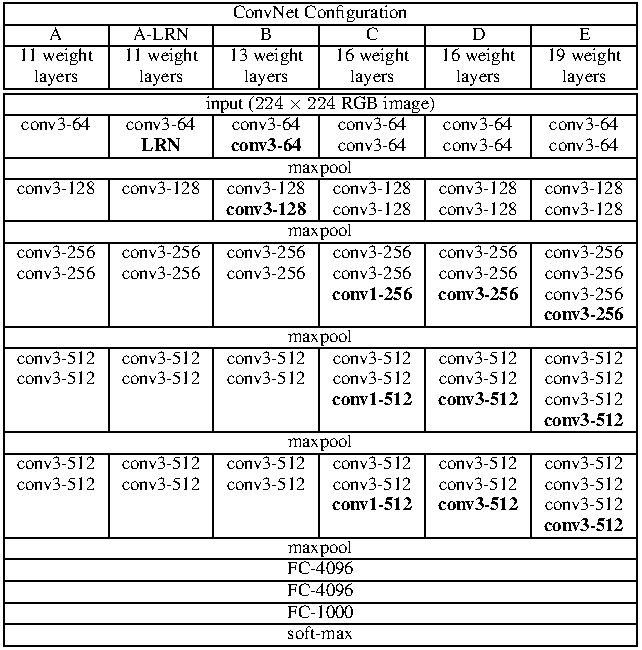
\includegraphics[width=0.8\textwidth]{Bilder/vgg16-architecture.pdf} 
	\caption{Die ursprünglichen VGG-Architekturen. Spalte D zeigt VGG16 wie in \autoref{sec:pretrained-backbones:vgg16} beschrieben. Abb. aus \cite{Simonyan.04092014}.}
	\label{fig:vgg16-architecture}
\end{figure} 

\begin{figure}
	\centering
	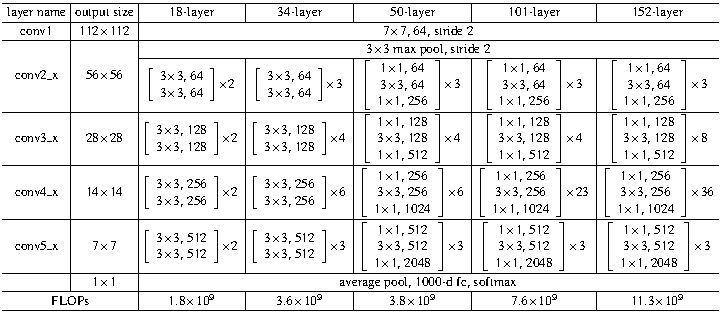
\includegraphics[width=0.8\textwidth]{Bilder/resnet34-architecture.pdf} 
	\caption{Die ursprünglichen ResNet-Architekturen. Zwischen jeweils zwei Convolutional-Layer befindet sich eine Skip-Connection \cite{He.10122015}.}
	\label{fig:resnet34-architecture}
\end{figure} 

\begin{figure}
	\centering
	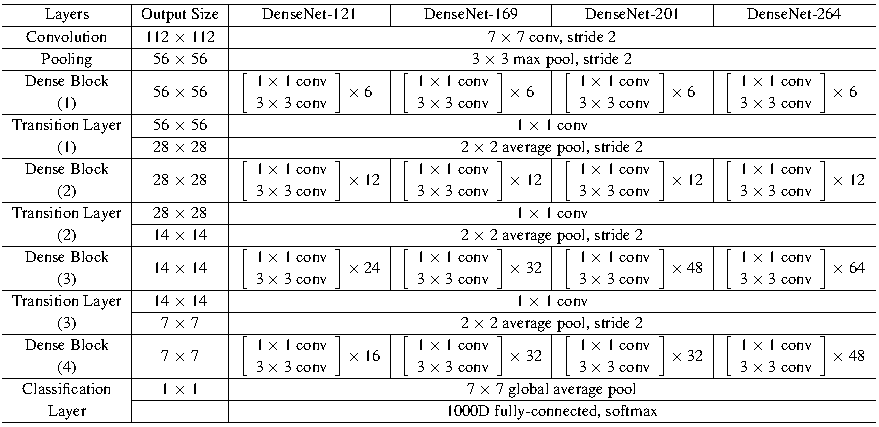
\includegraphics[width=0.8\textwidth]{Bilder/densenet121-architecture.pdf} 
	\caption{Die ursprünglichen DenseNet-Architekturen \cite{Huang.25082016}.}
	\label{fig:densenet121-architecture}
\end{figure} 

\pagebreak

\section{Quelltext-Implementation}

\lstinputlisting[
	label=code:quality,    % Label; genutzt für Referenzen auf dieses Code-Beispiel
	caption=Implementation des Quality-Maßes in Python zur Verwendung im Training und Testen von Keras-Modellen.,
	captionpos=b,               % Position, an der die Caption angezeigt wird t(op) oder b(ottom)
	style=EigenerPythonStyle,   % Eigener Style der vor dem Dokument festgelegt wurde
	firstline=1,                % Zeilennummer im Dokument welche als erste angezeigt wird
	lastline=50                 % Letzte Zeile welche ins LaTeX Dokument übernommen wird
]{Quellcode/quality.py}

\pagebreak 

\section{Beispiel-Predictions Combined}


\begin{figure}
	\centering
	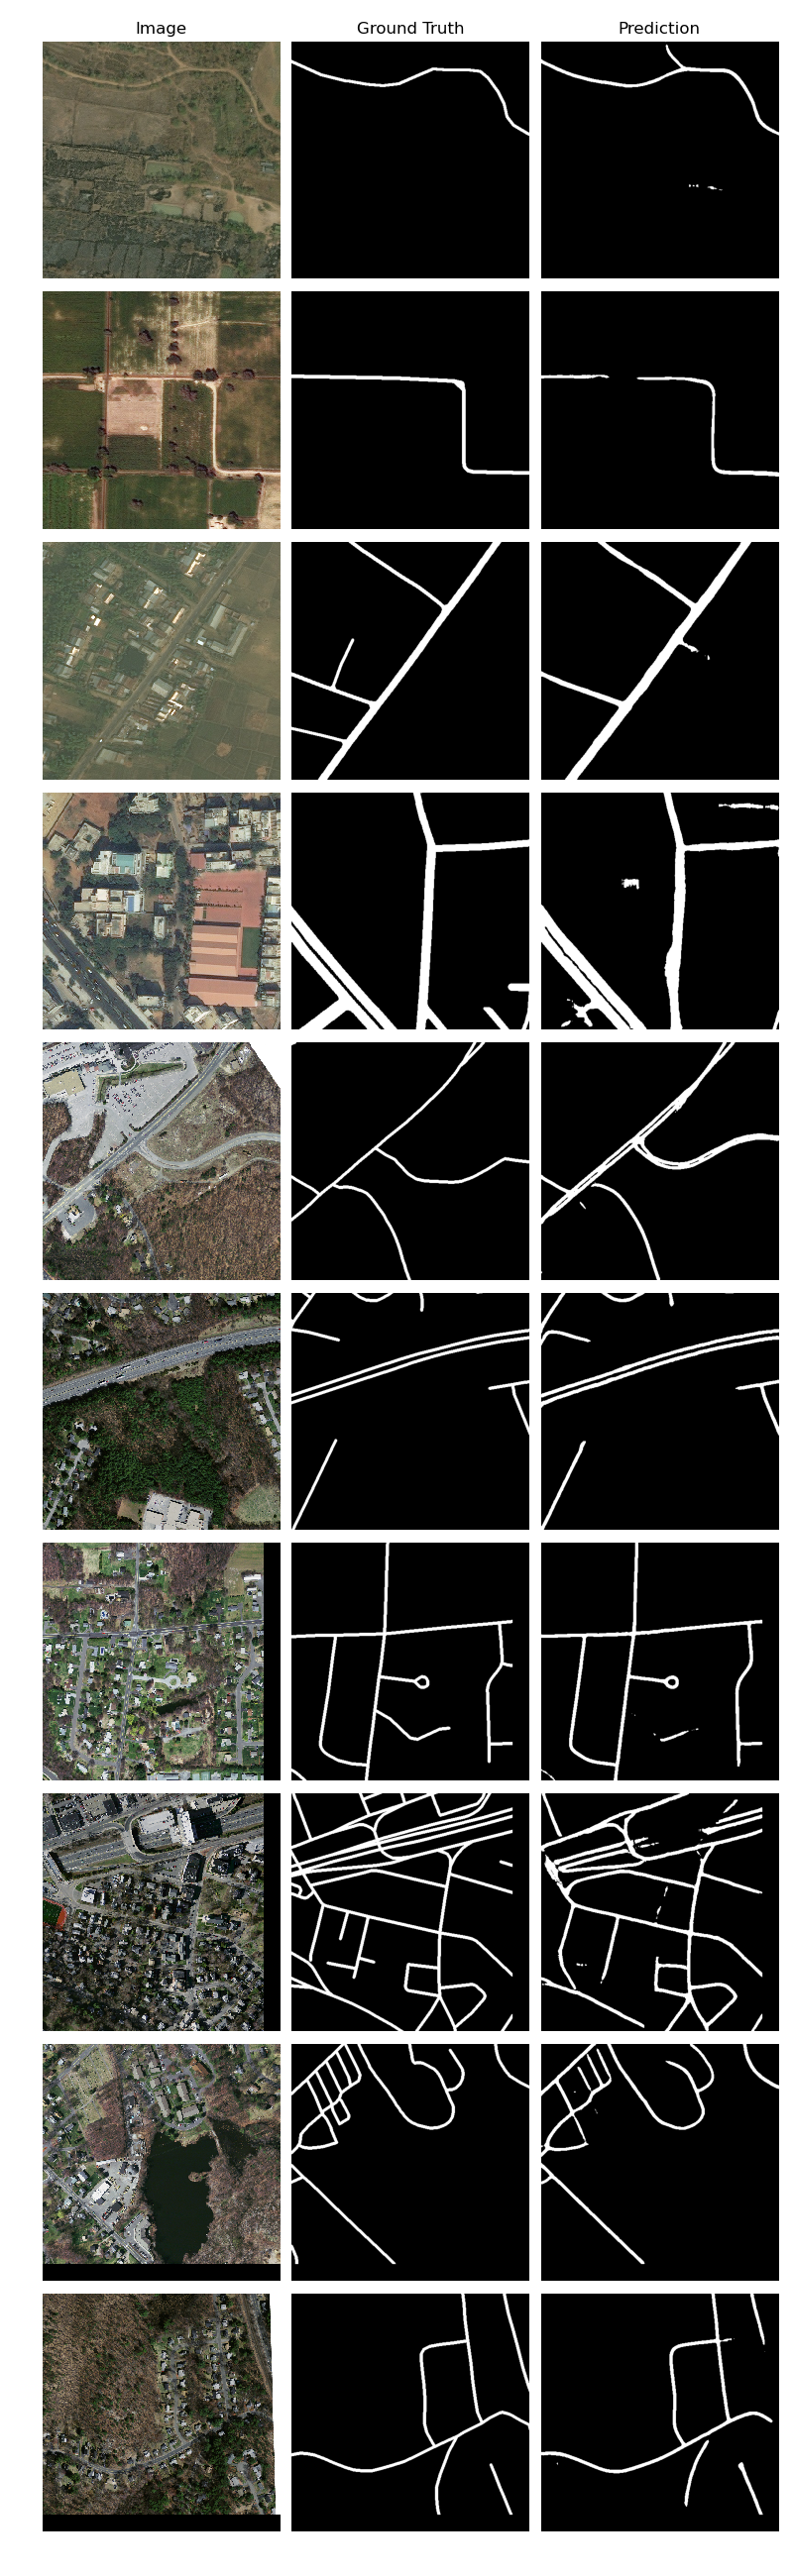
\includegraphics[width=.41\textwidth]{Bilder/Samples-Combined/bunet15.png}
	\caption{Beispiel-Predictions des $BUNet15$ auf dem Combined-Datensatz.}
	\label{fig:combined-samples-bunet15}
\end{figure}

\begin{figure}
	\centering
	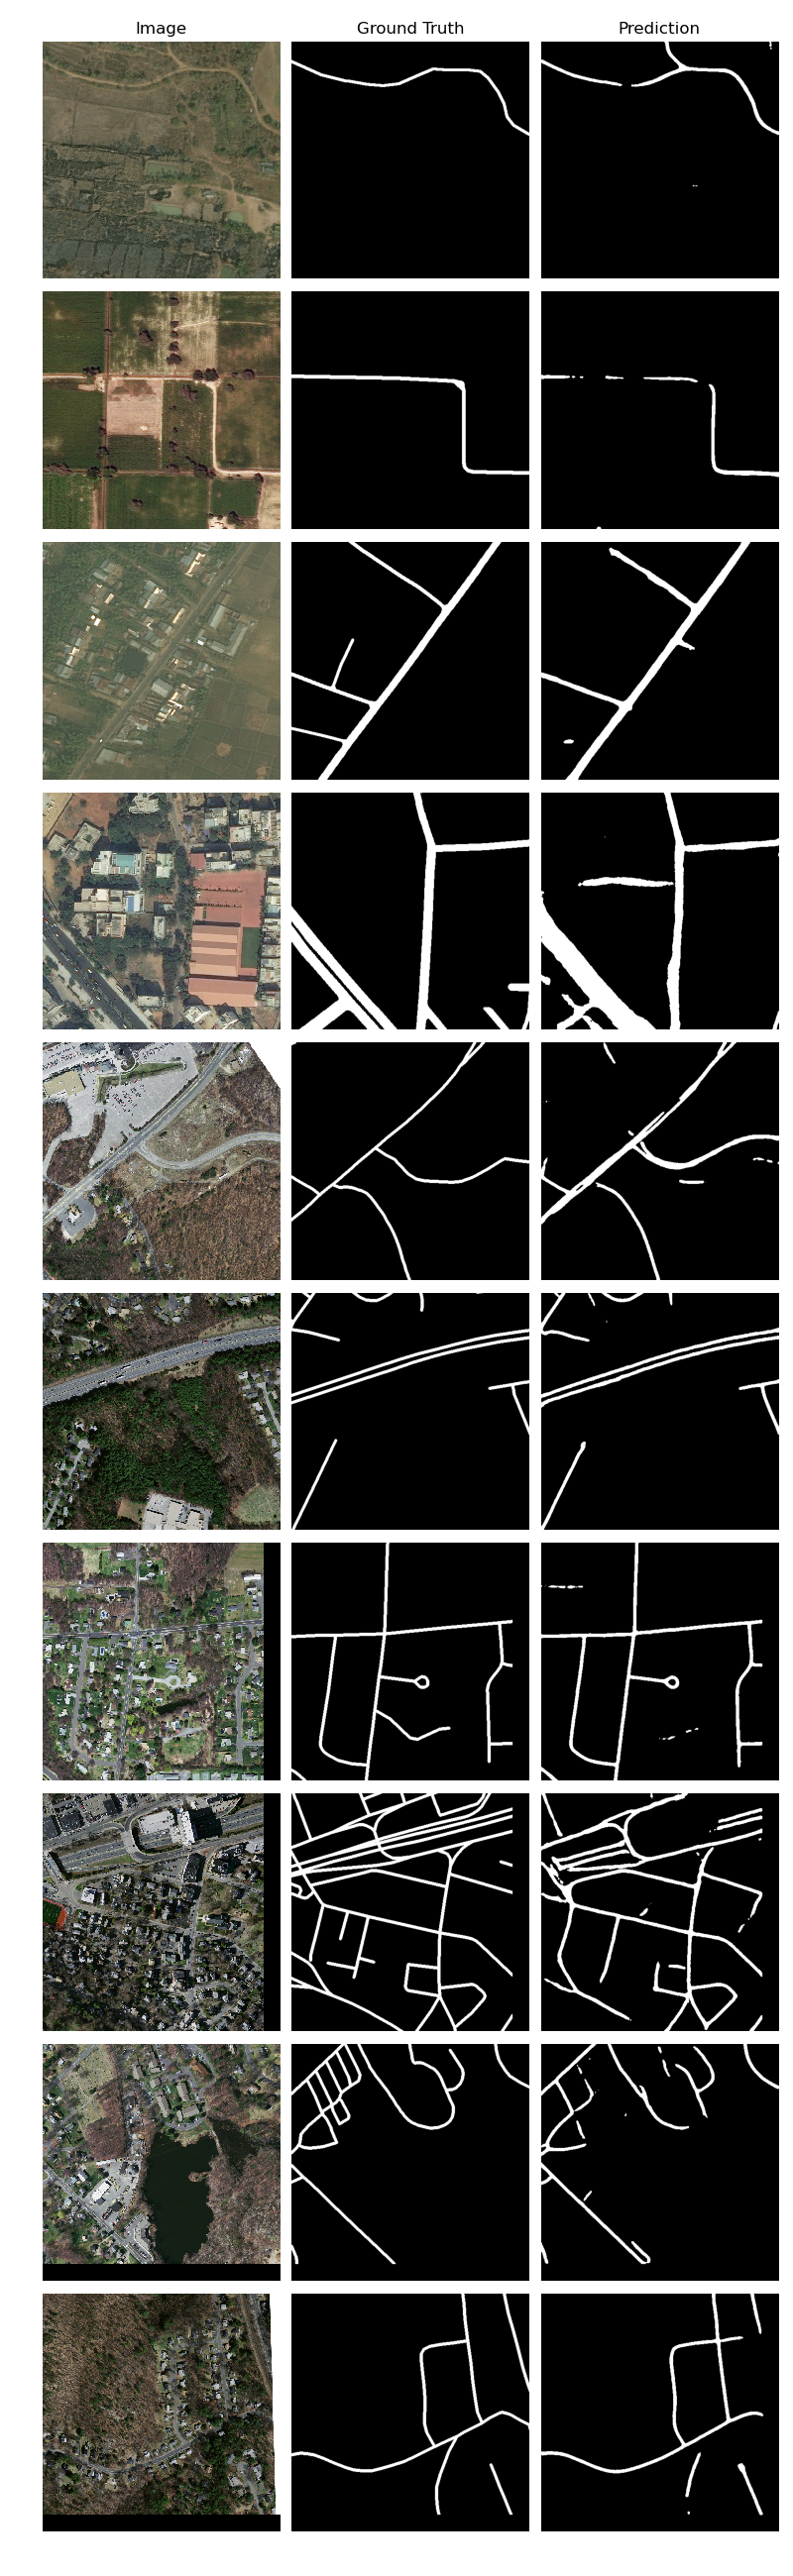
\includegraphics[width=.41\textwidth]{Bilder/Samples-Combined/bunet2.png}
	\caption{Beispiel-Predictions des $BUNet2$ auf dem Combined-Datensatz.}
	\label{fig:combined-samples-bunet2}
\end{figure}

\begin{figure}
	\centering
	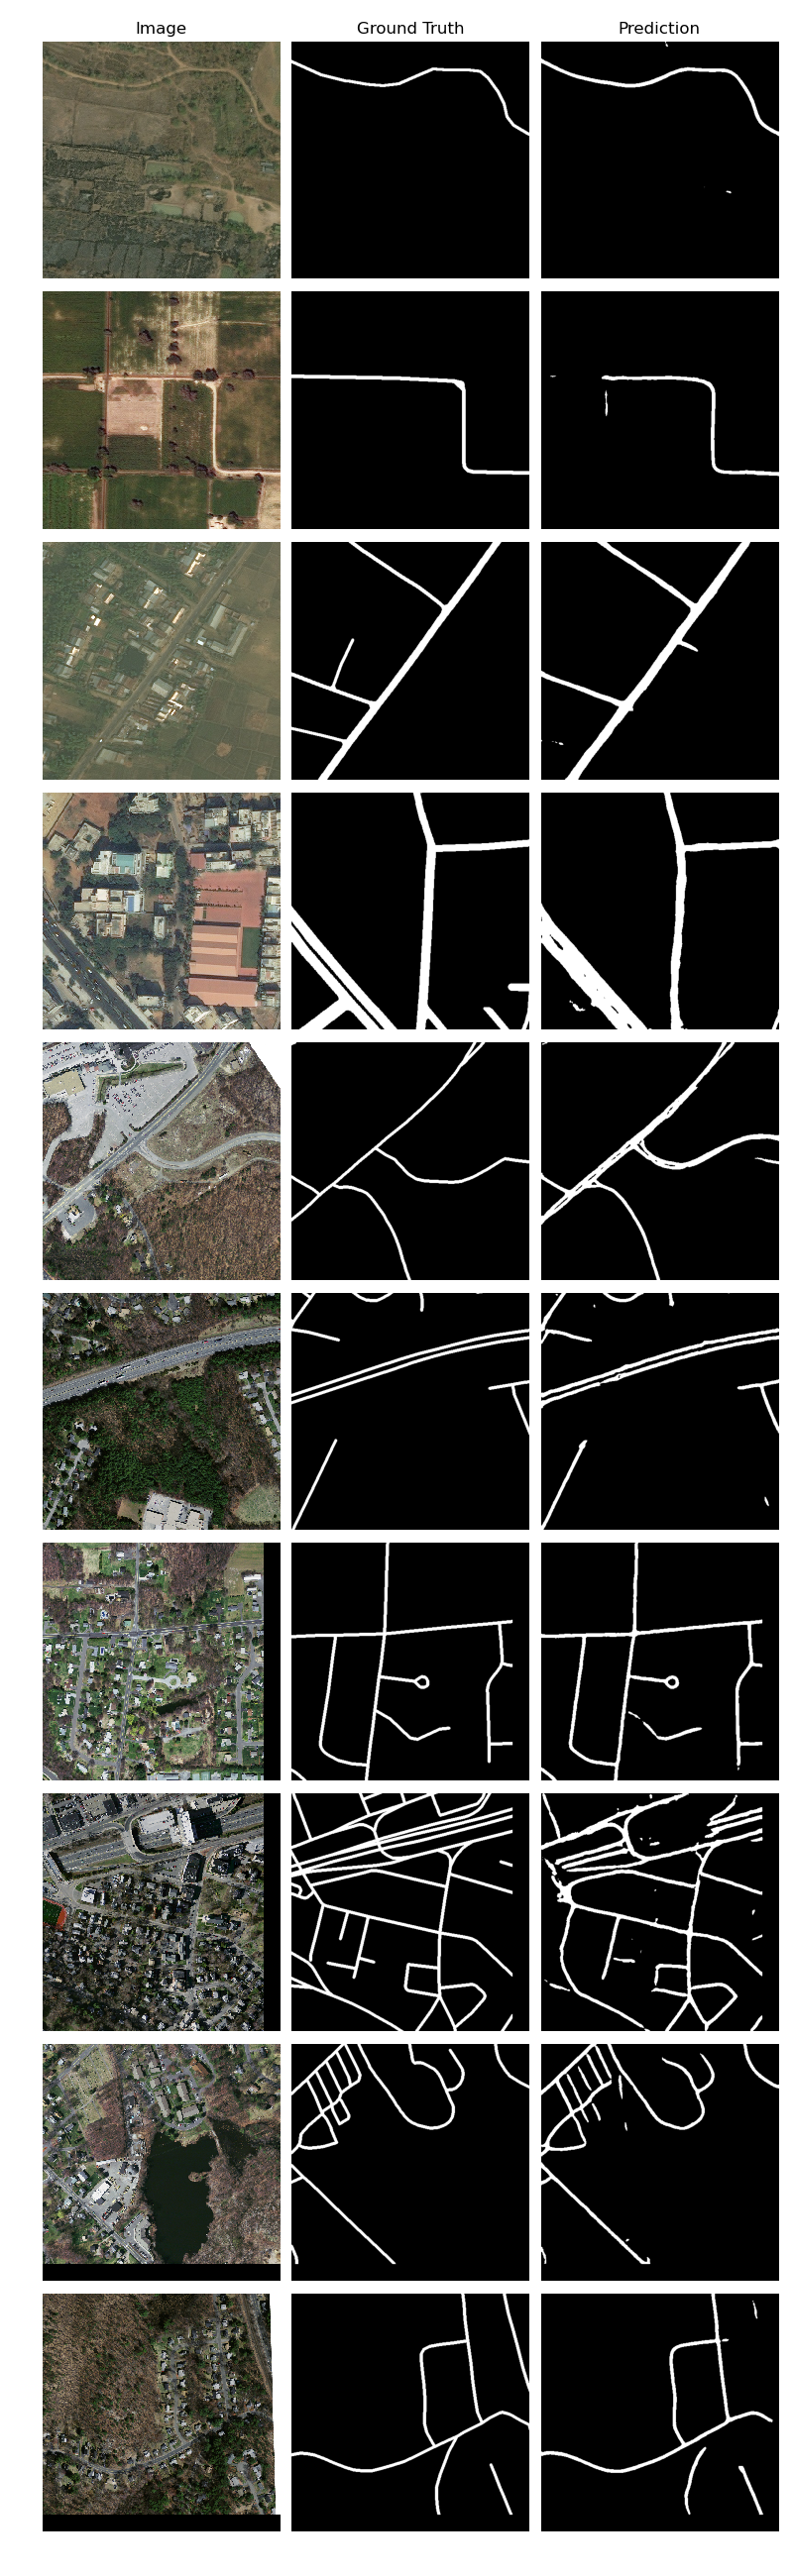
\includegraphics[width=.41\textwidth]{Bilder/Samples-Combined/dbunet.png}
	\caption{Beispiel-Predictions des $DBUNet$ auf dem Combined-Datensatz.}
	\label{fig:combined-samples-dbunet}
\end{figure}

\begin{figure}
	\centering
	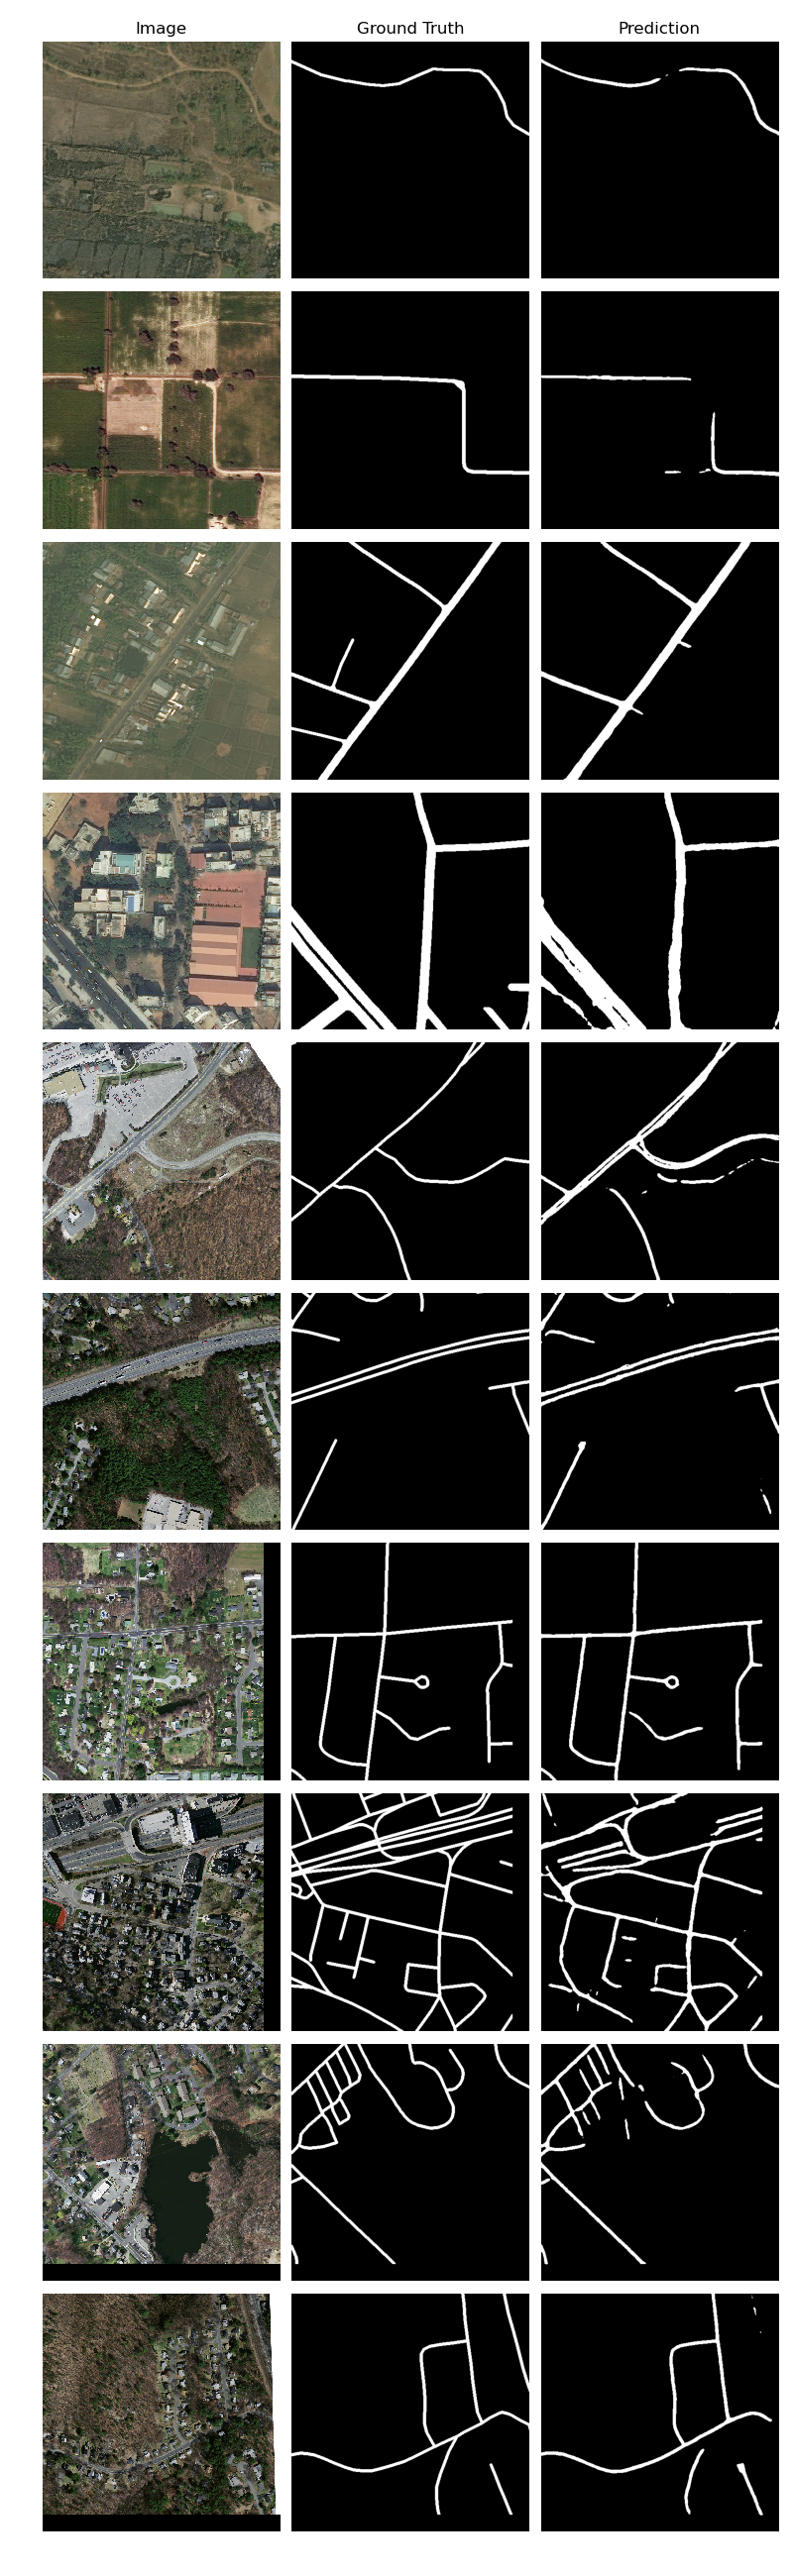
\includegraphics[width=.41\textwidth]{Bilder/Samples-Combined/rbunet.png}
	\caption{Beispiel-Predictions des $RBUNet$ auf dem Combined-Datensatz.}
	\label{fig:combined-samples-rbunet}
\end{figure}

\begin{figure}
	\centering
	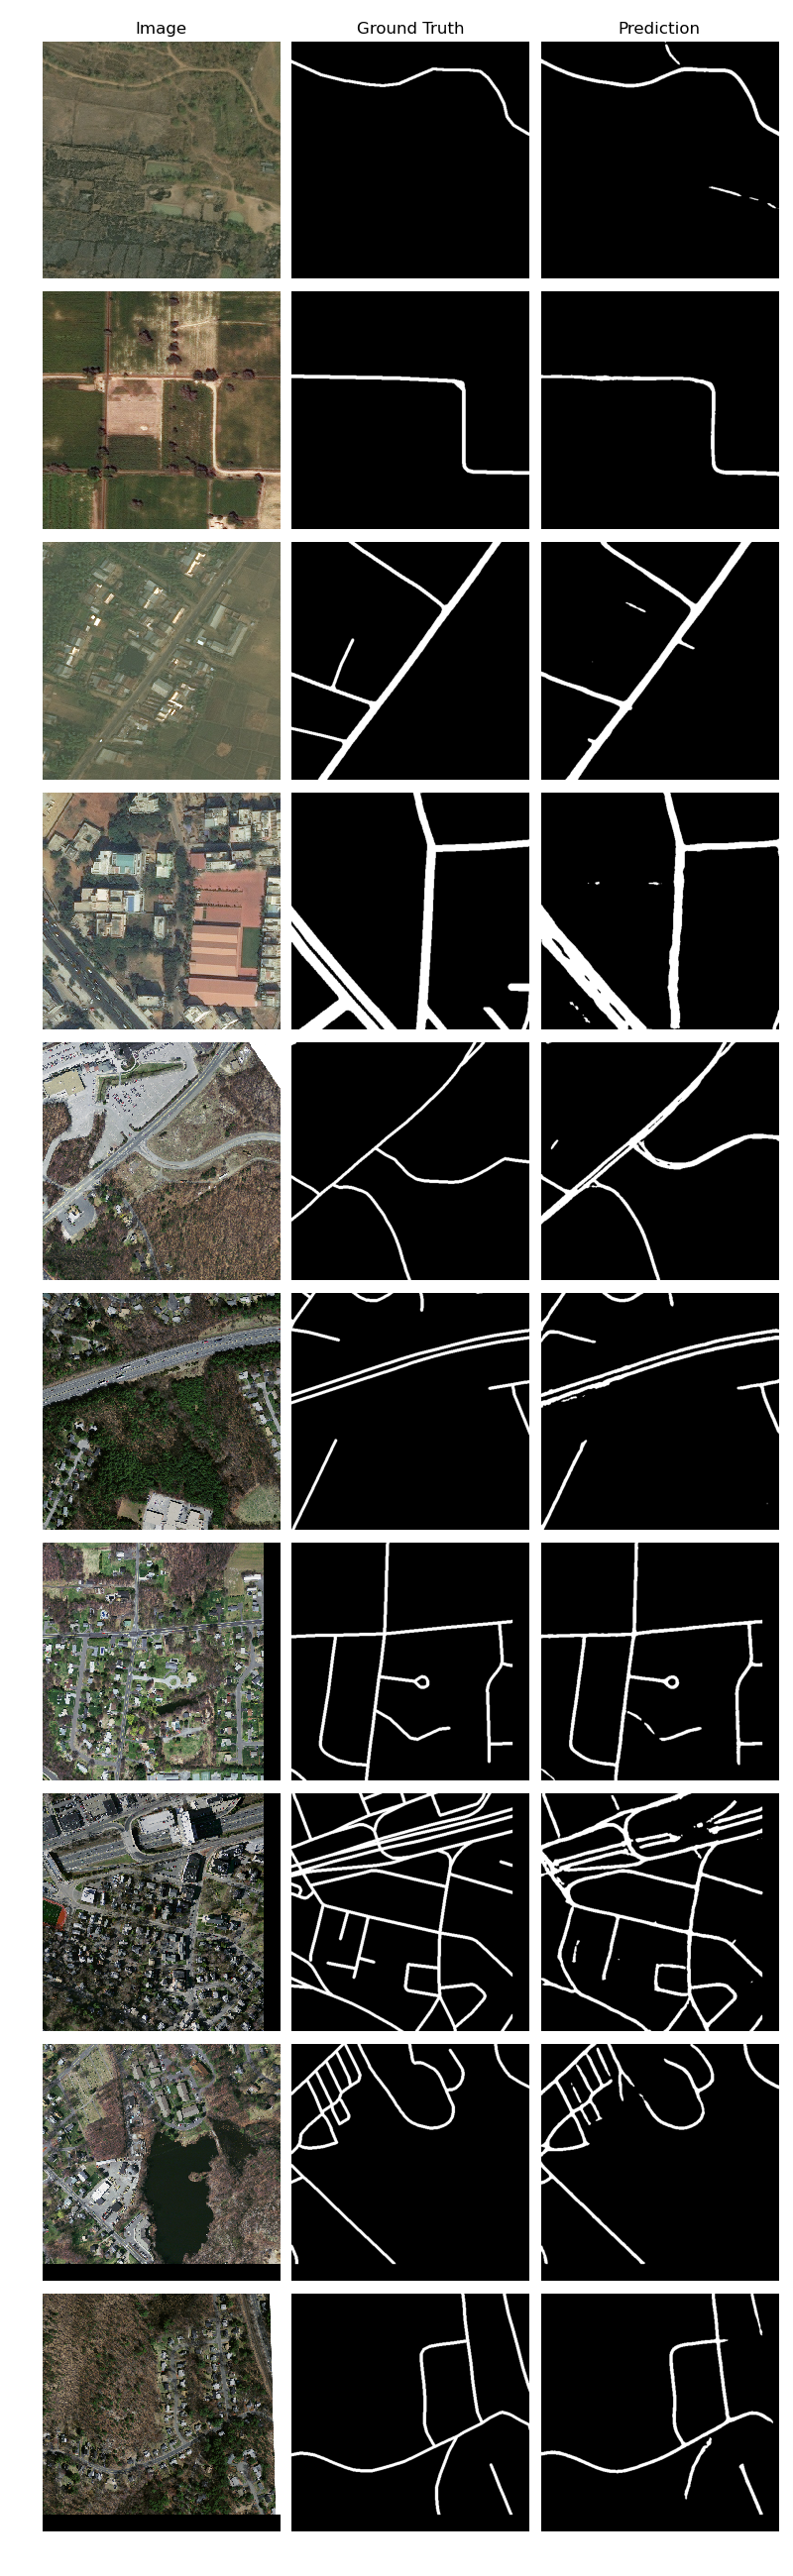
\includegraphics[width=.41\textwidth]{Bilder/Samples-Combined/vbunet.png}
	\caption{Beispiel-Predictions des $VBUNet$ auf dem Combined-Datensatz.}
	\label{fig:combined-samples-vbunet}
\end{figure}

\pagebreak 



\section{Beispiel-Predictions BikeSat}

\begin{figure}
	\centering
	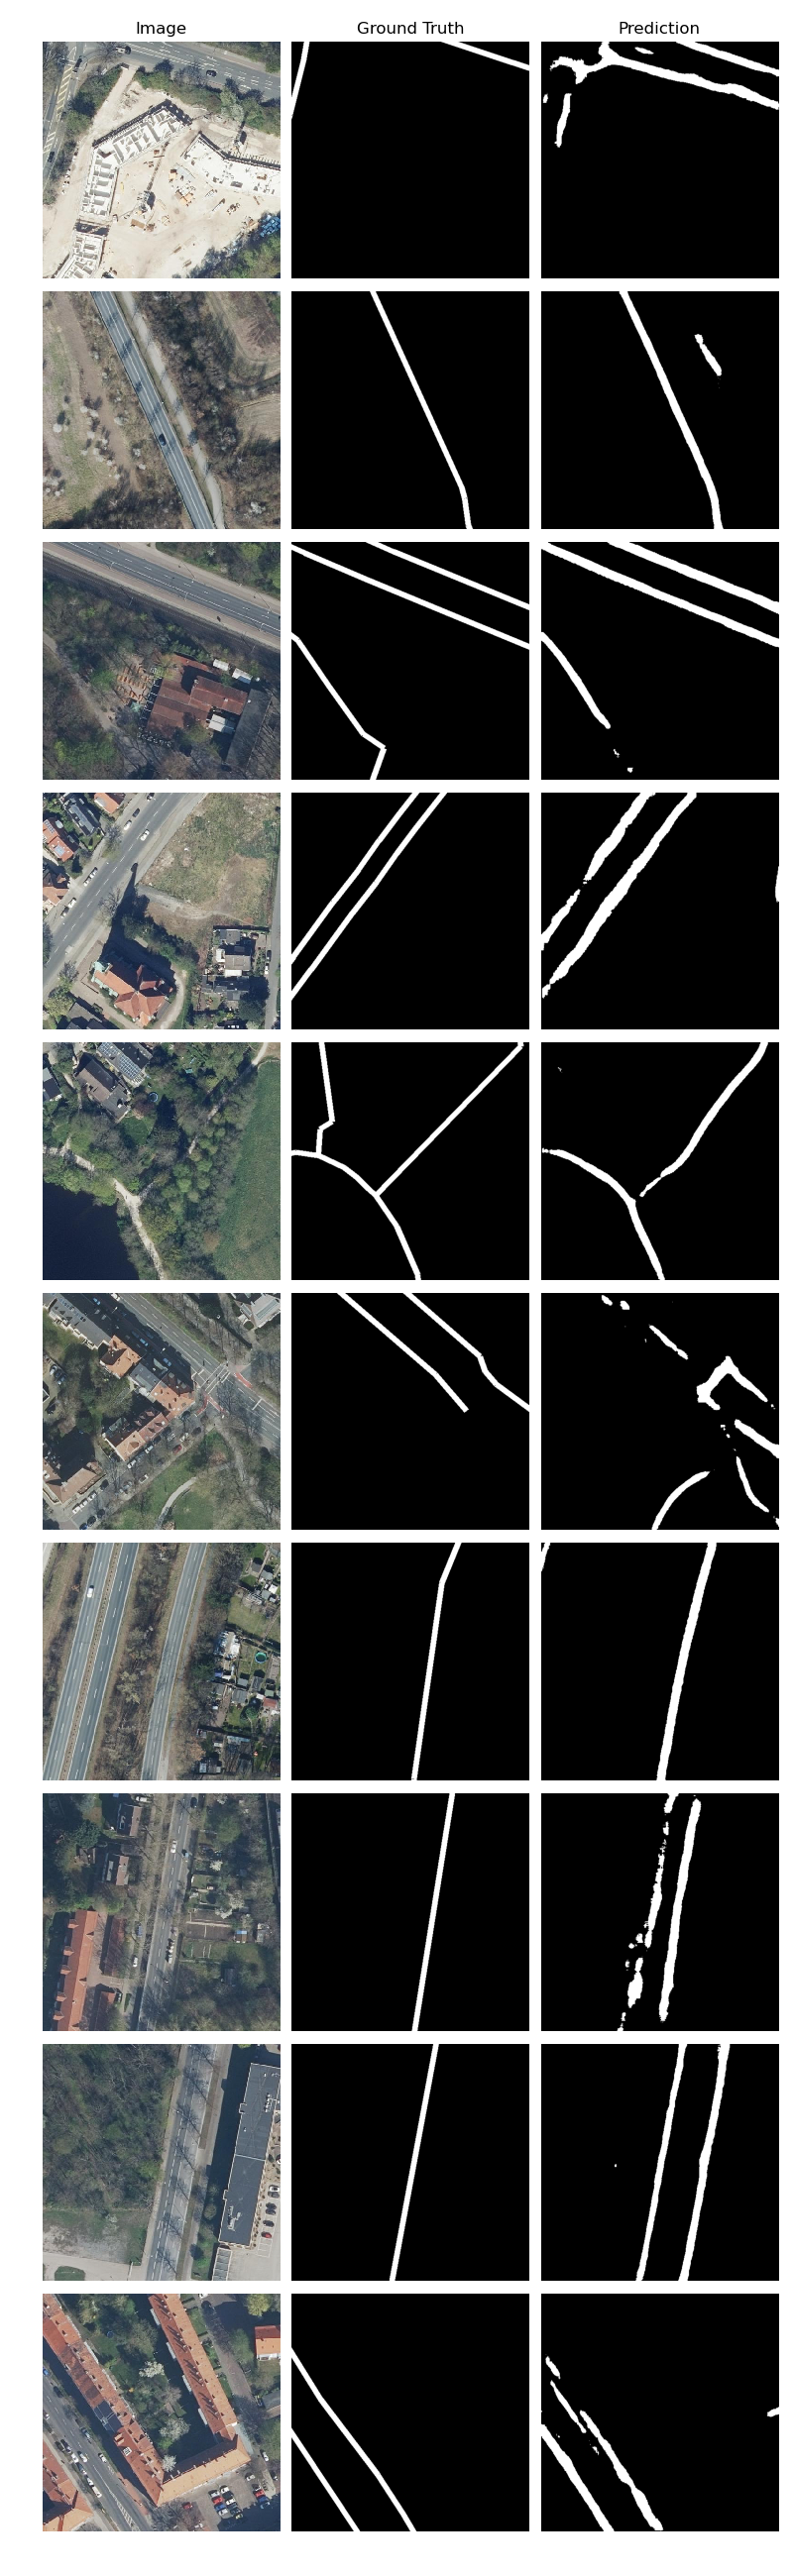
\includegraphics[width=.41\textwidth]{Bilder/Samples-BikeSat/bunet15-l.png} 
	\caption{Beispiel-Predictions des $BUNet15^l$ auf dem BikeSat-Datensatz.}
	\label{fig:bikesat-samples-bunet15-l}
\end{figure}

\begin{figure}
	\centering
	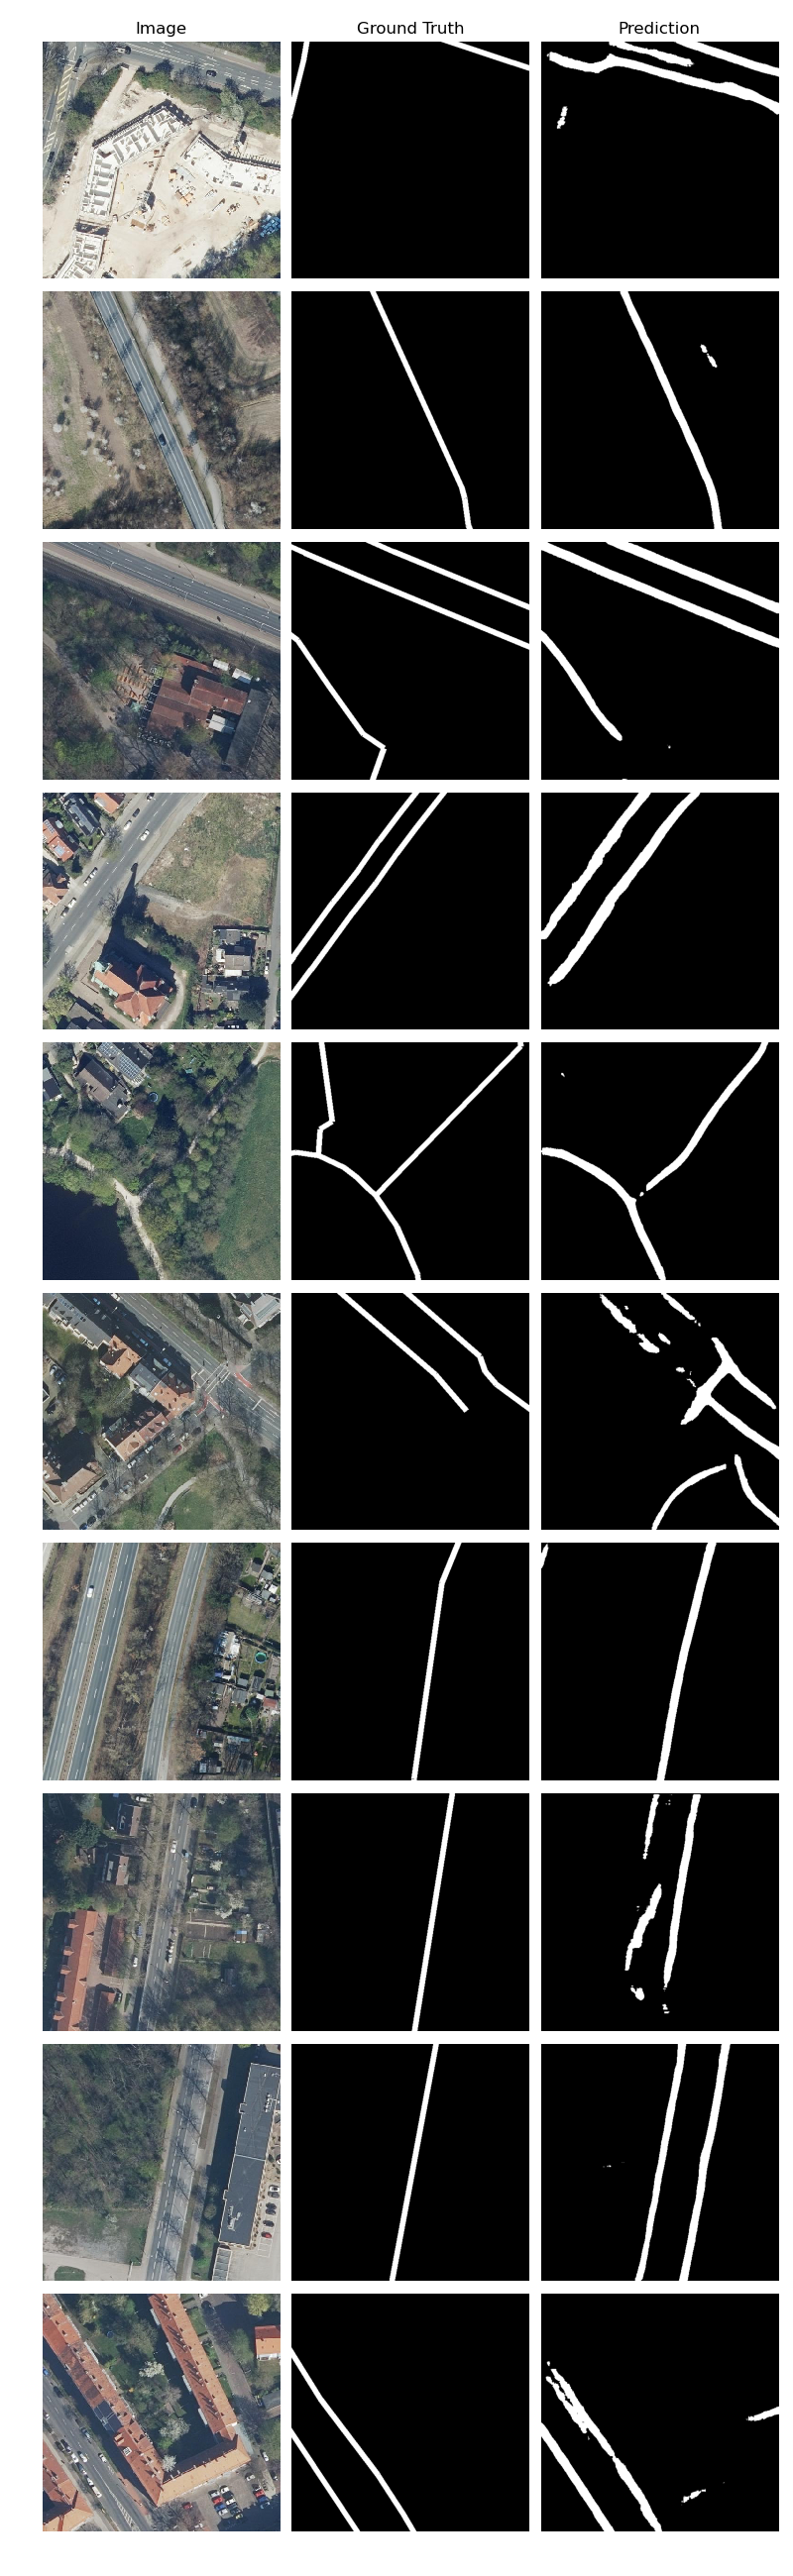
\includegraphics[width=.41\textwidth]{Bilder/Samples-BikeSat/bunet15-r.png} 
	\caption{Beispiel-Predictions des $BUNet15^r$ auf dem BikeSat-Datensatz.}
	\label{fig:bikesat-samples-bunet15-r}
\end{figure}

\begin{figure}
	\centering
	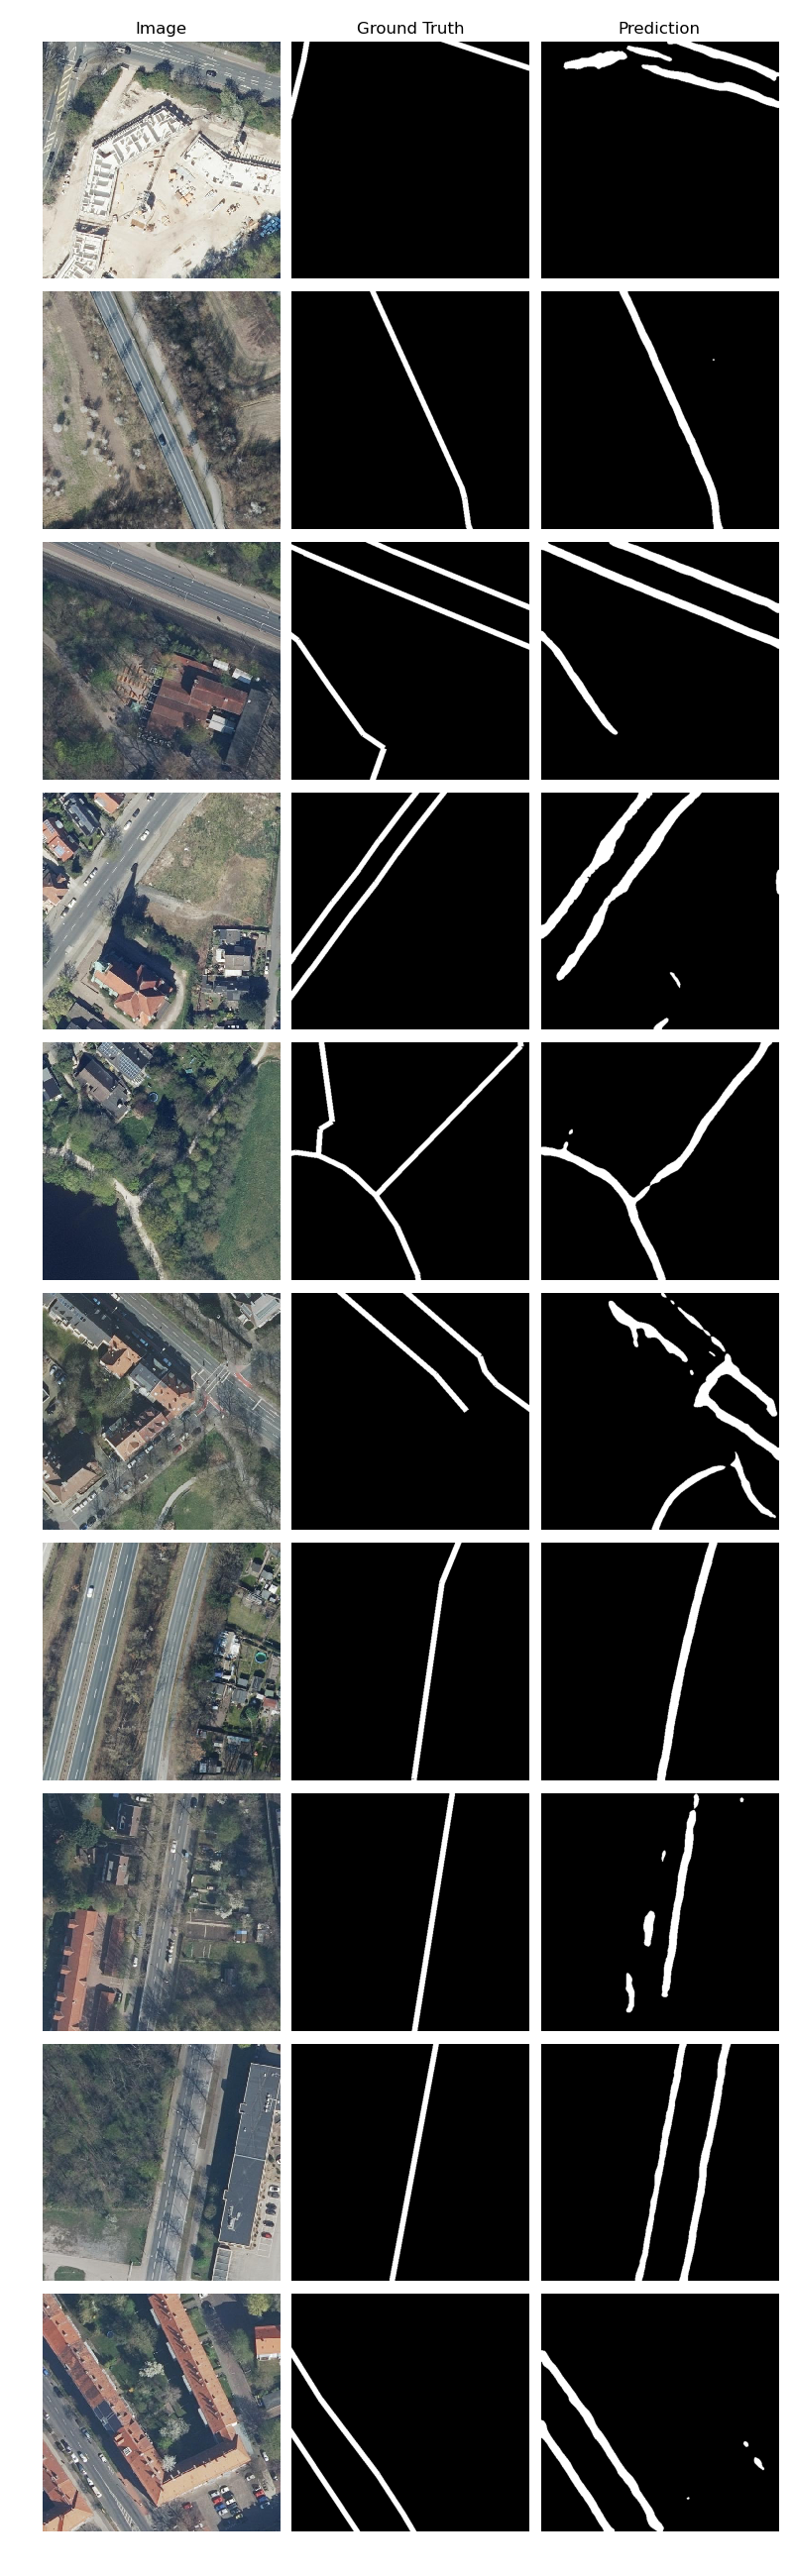
\includegraphics[width=.41\textwidth]{Bilder/Samples-BikeSat/bunet15-s.png} 
	\caption{Beispiel-Predictions des $BUNe15t^*$ auf dem BikeSat-Datensatz.}
	\label{fig:bikesat-samples-bunet15-s}
\end{figure}

\begin{figure}
	\centering
	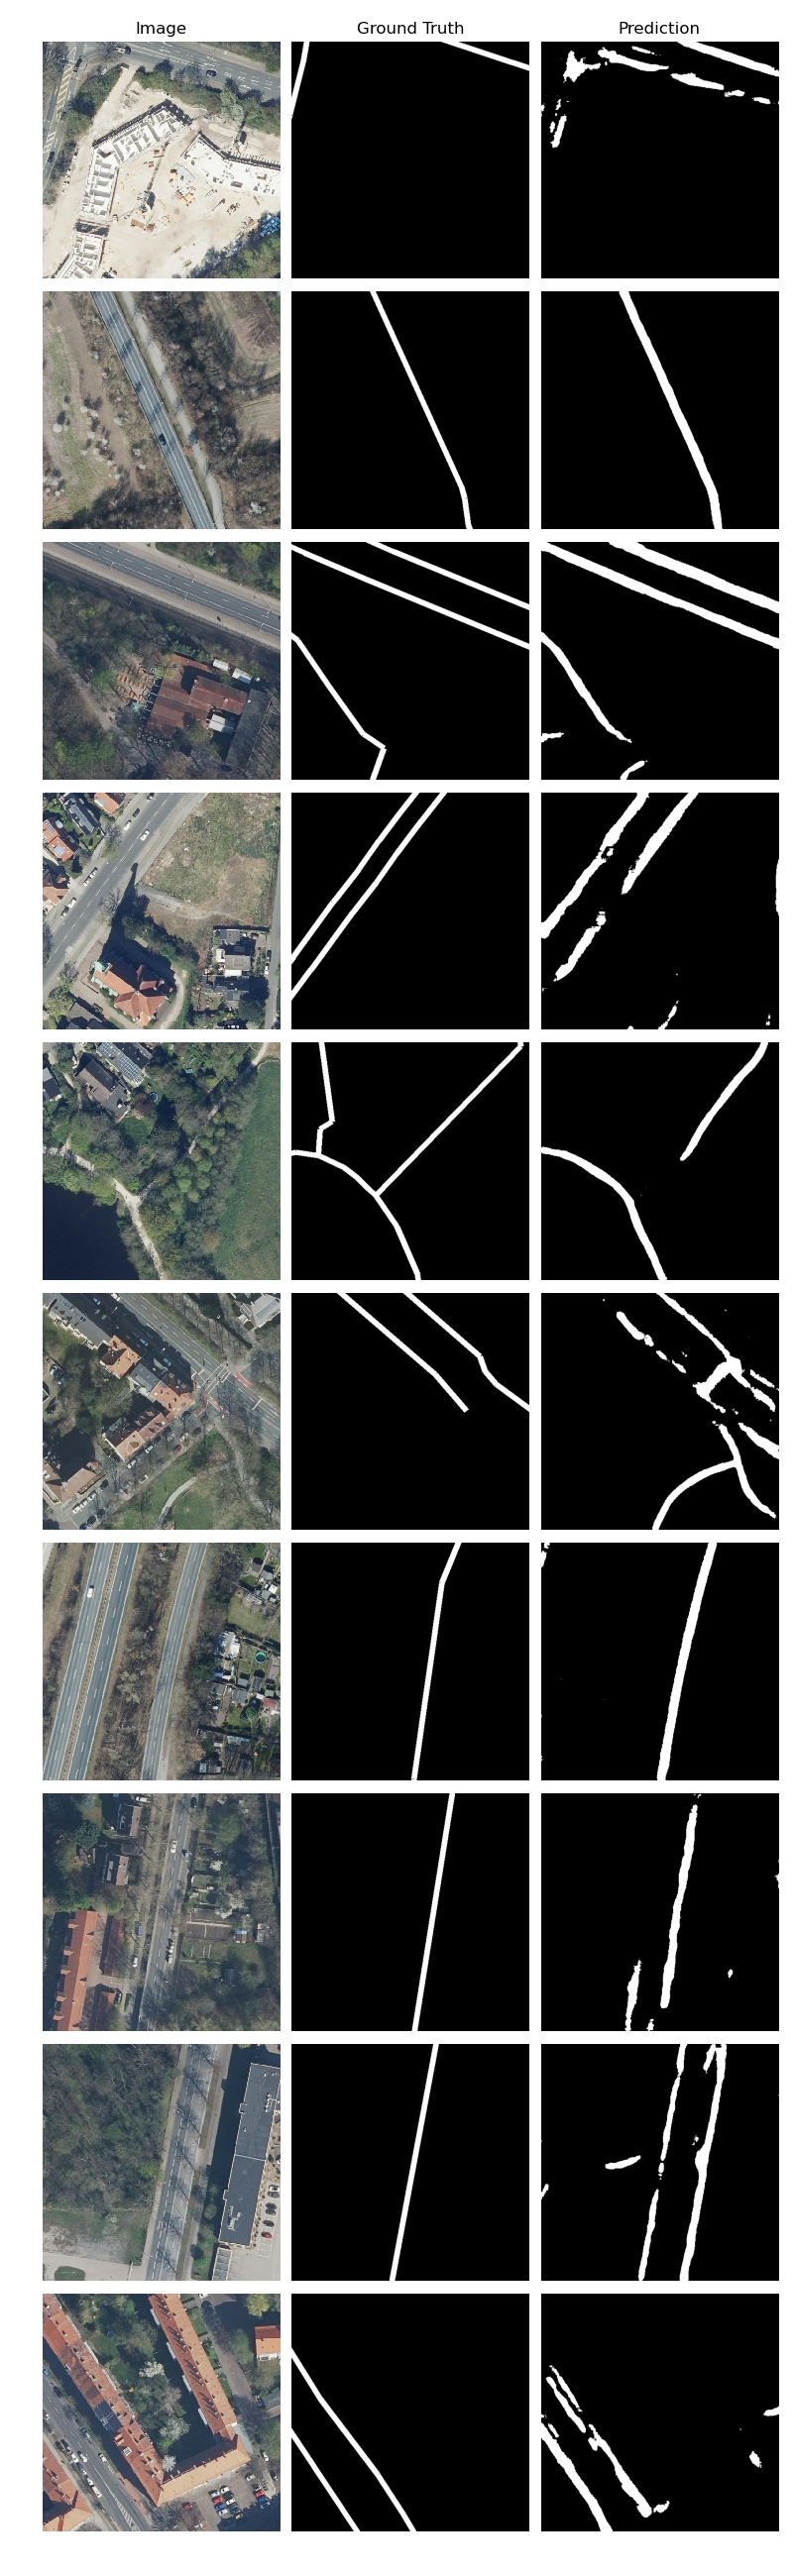
\includegraphics[width=.41\textwidth]{Bilder/Samples-BikeSat/bunet2-l.png} 
	\caption{Beispiel-Predictions des $BUNet2^l$ auf dem BikeSat-Datensatz.}
	\label{fig:bikesat-samples-bunet2-l}
\end{figure}

\begin{figure}
	\centering
	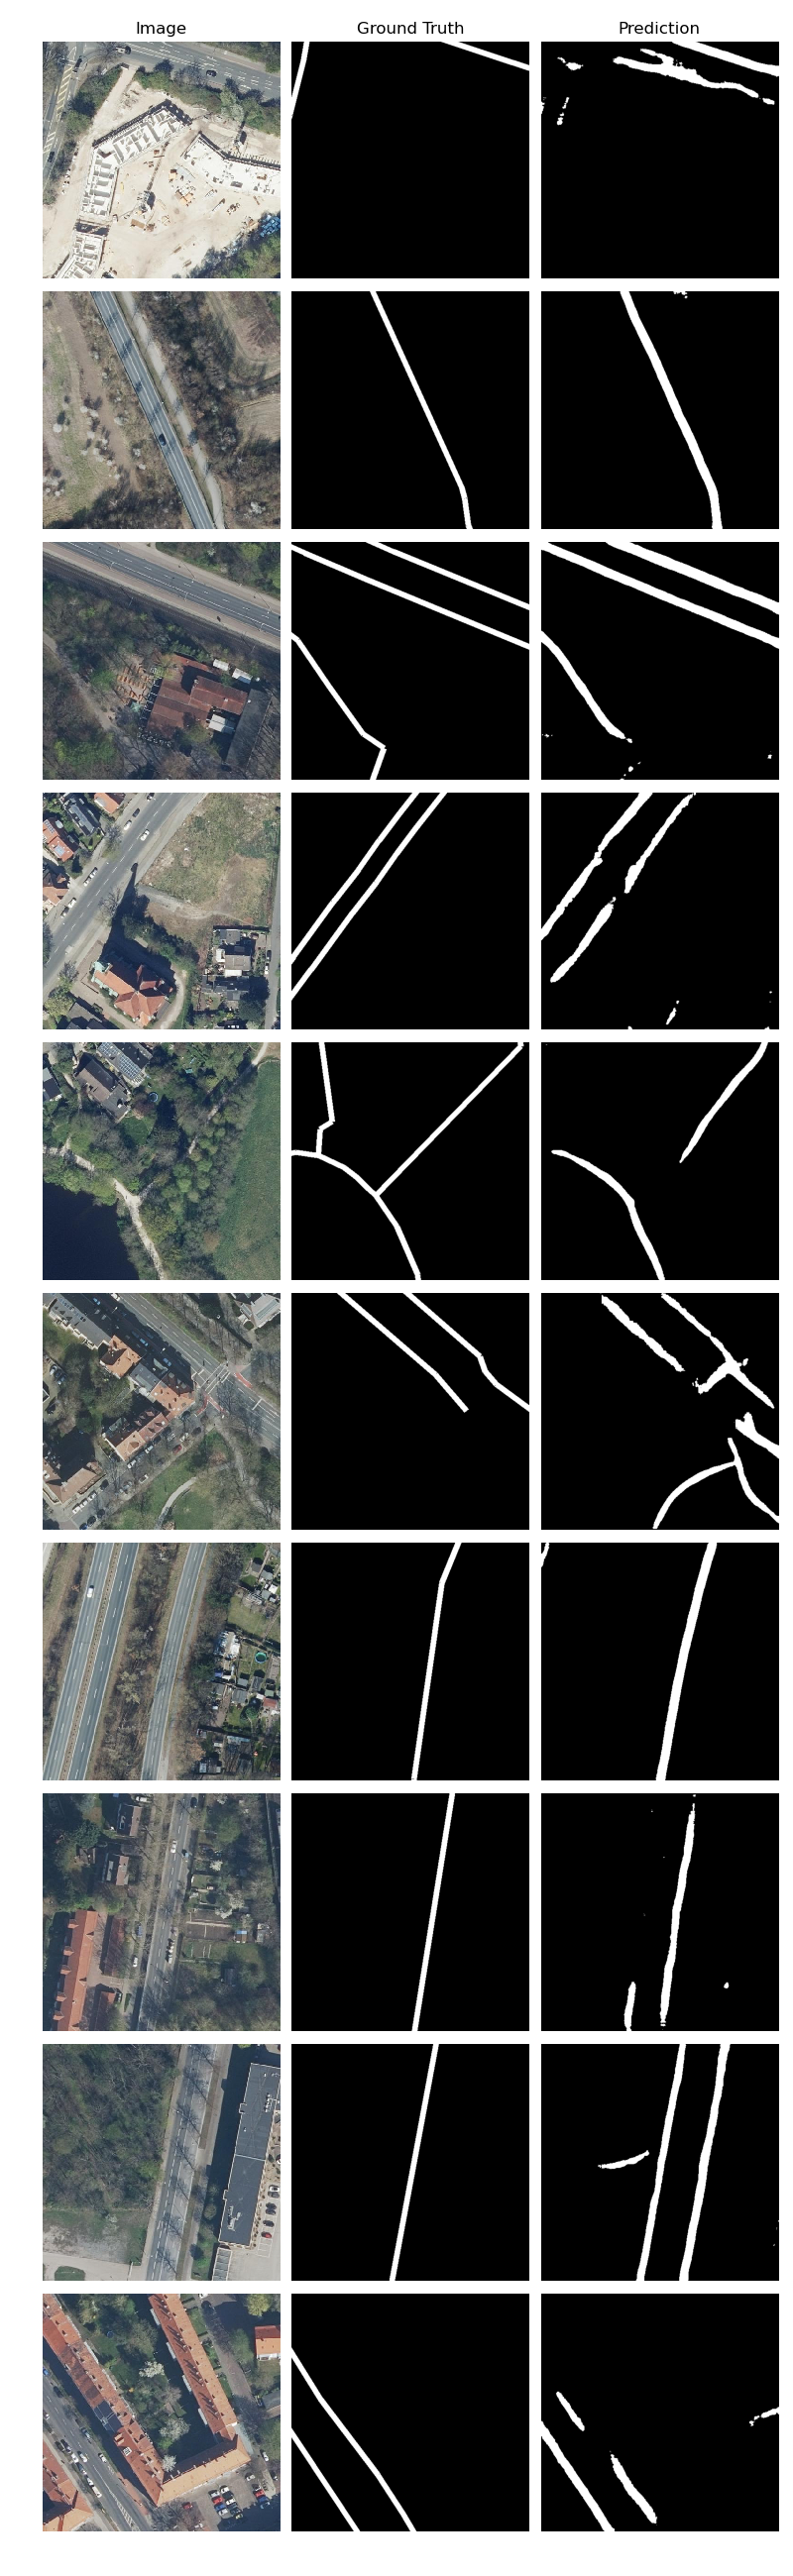
\includegraphics[width=.41\textwidth]{Bilder/Samples-BikeSat/bunet2-r.png} 
	\caption{Beispiel-Predictions des $BUNet2^r$ auf dem BikeSat-Datensatz.}
	\label{fig:bikesat-samples-bunet2-r}
\end{figure}

\begin{figure}
	\centering
	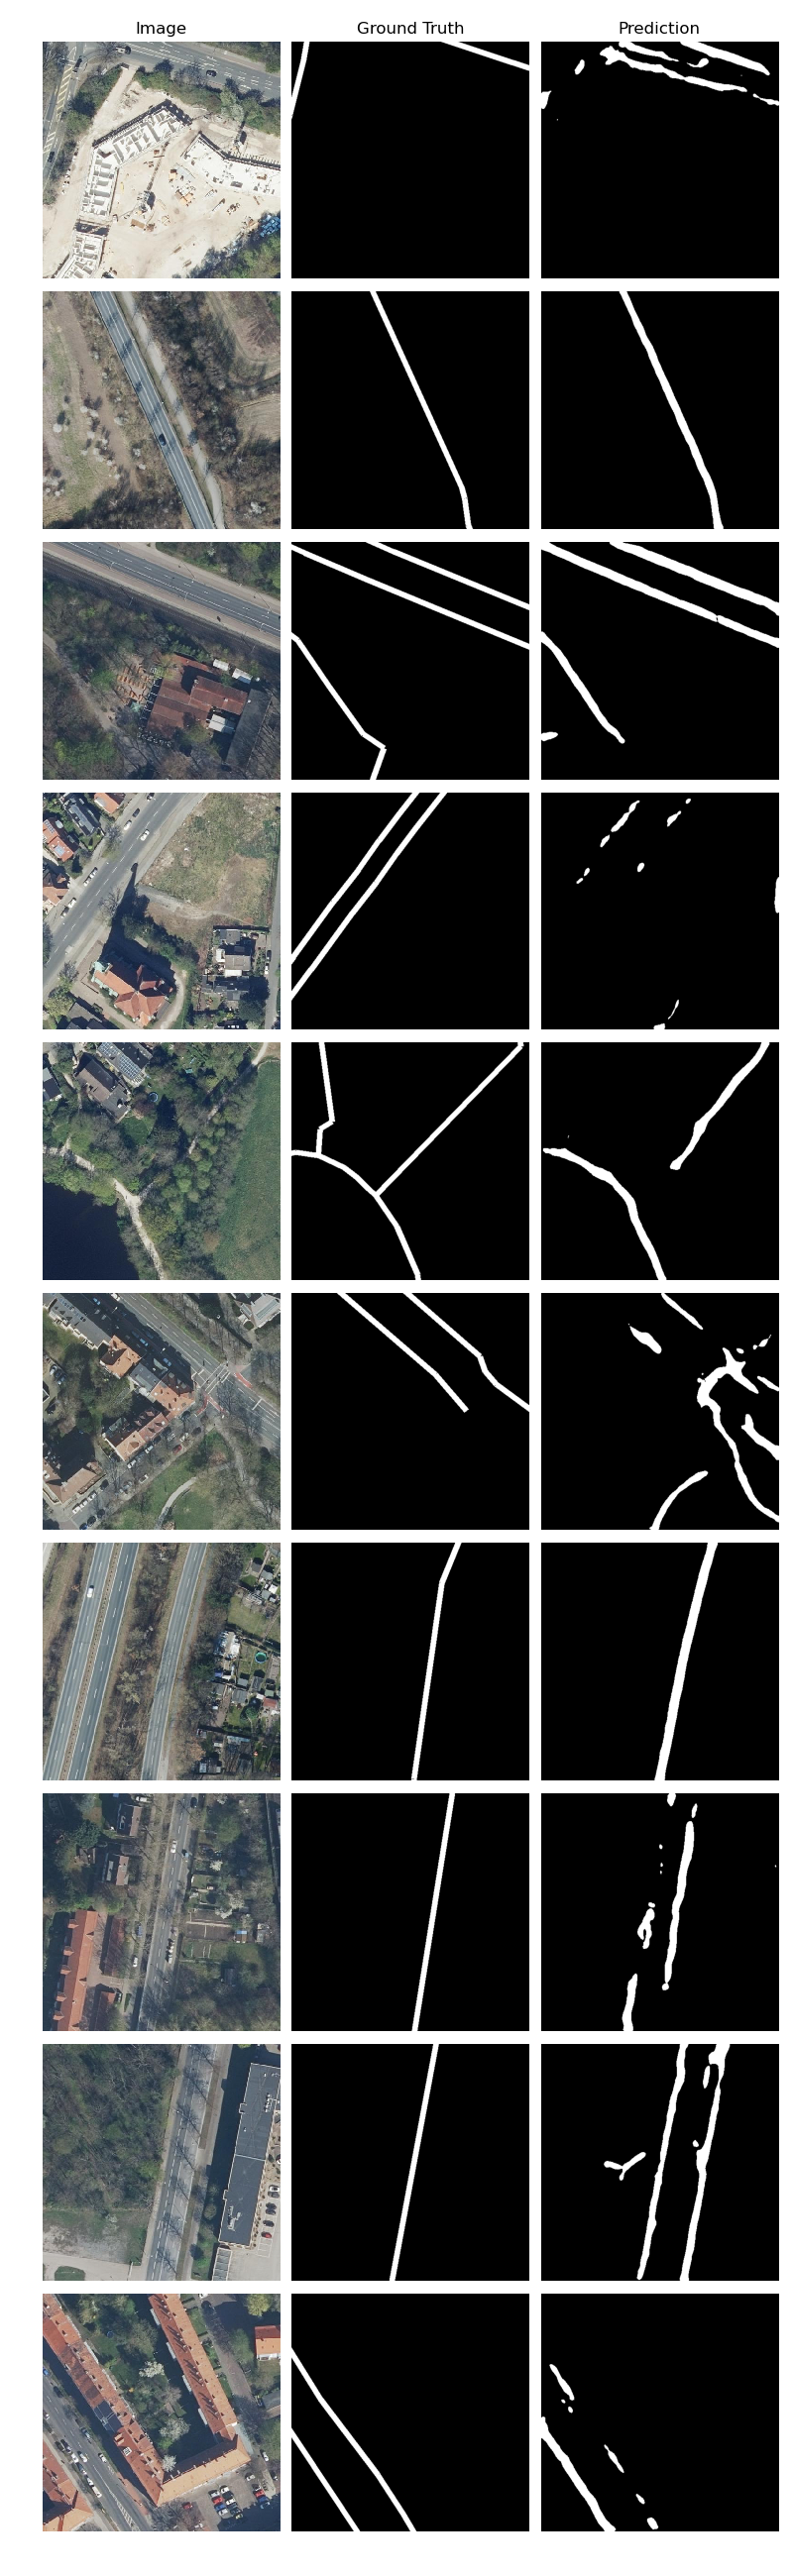
\includegraphics[width=.41\textwidth]{Bilder/Samples-BikeSat/bunet2-s.png} 
	\caption{Beispiel-Predictions des $BUNet2^*$ auf dem BikeSat-Datensatz.}
	\label{fig:bikesat-samples-bunet2-s}
\end{figure}

\begin{figure}
	\centering
	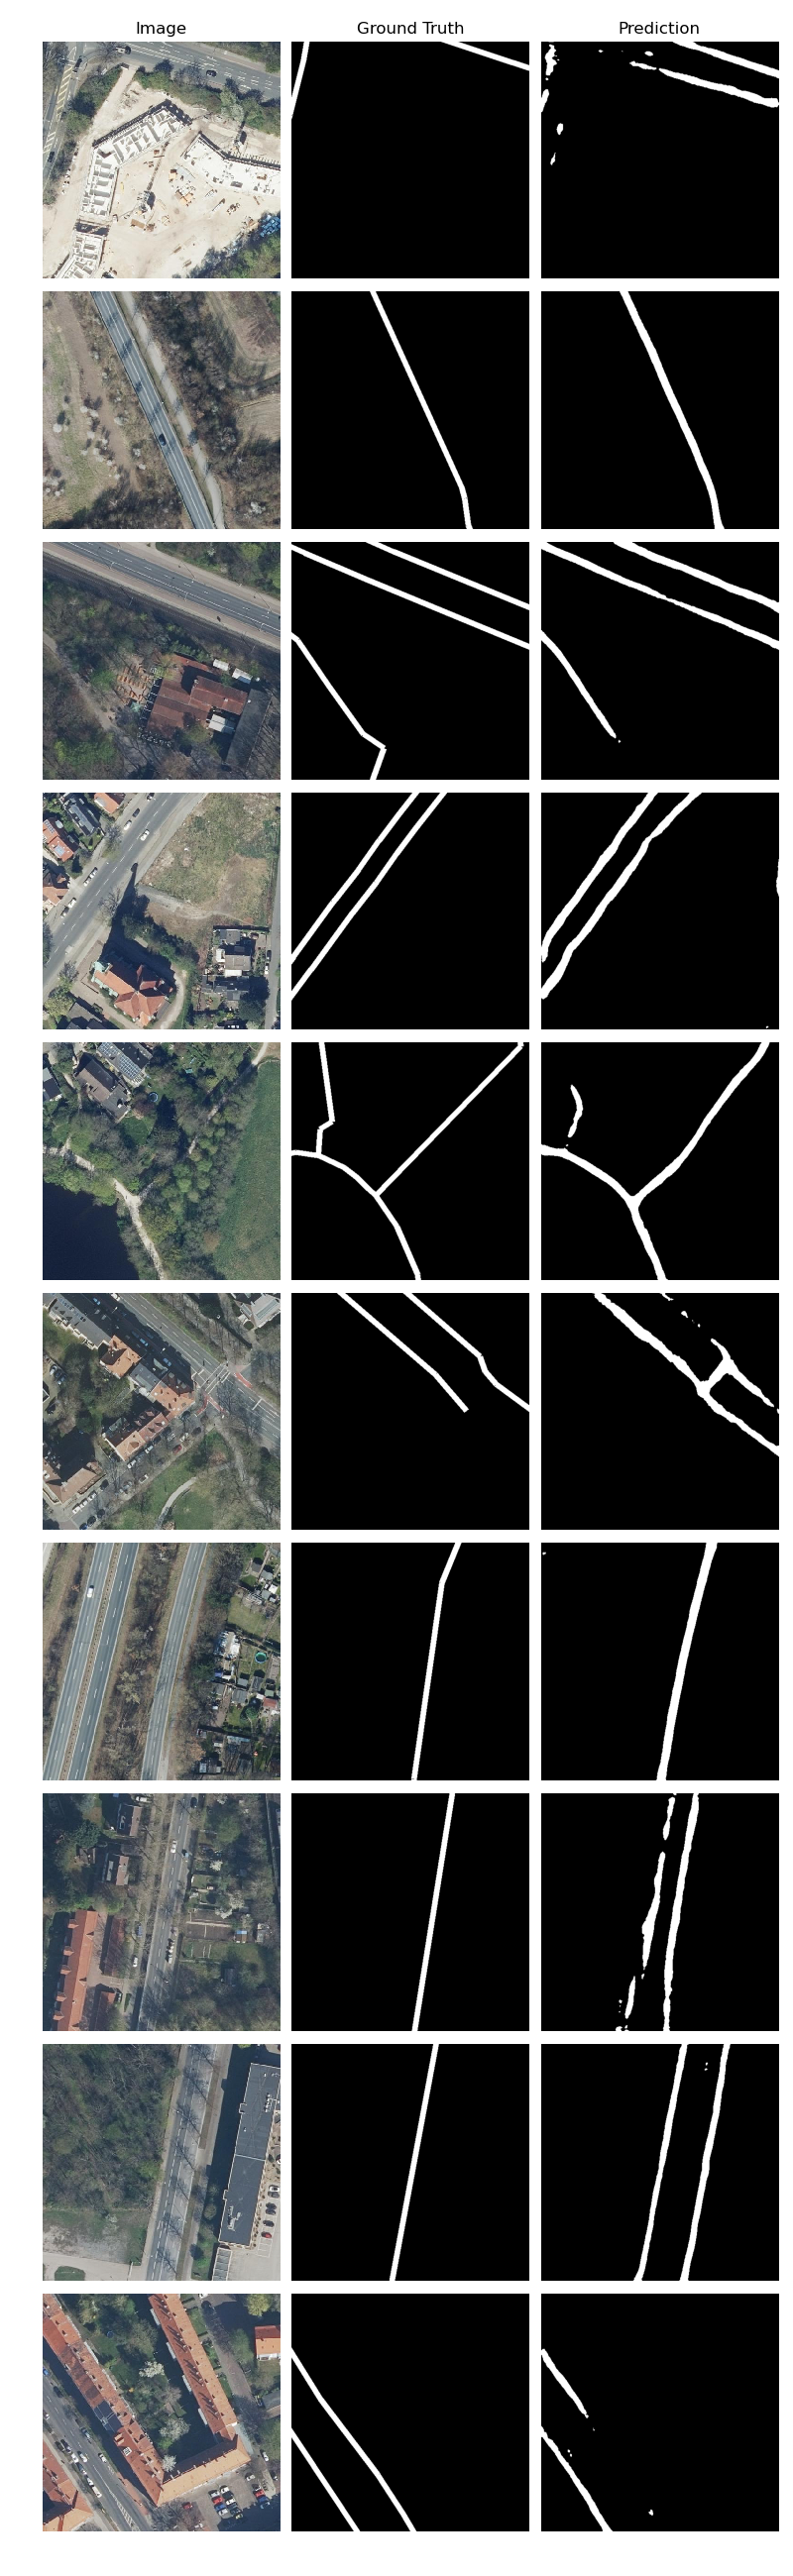
\includegraphics[width=.41\textwidth]{Bilder/Samples-BikeSat/dbunet-l.png} 
	\caption{Beispiel-Predictions des $DBUNet^l$ auf dem BikeSat-Datensatz.}
	\label{fig:bikesat-samples-dbunet-l}
\end{figure}

\begin{figure}
	\centering
	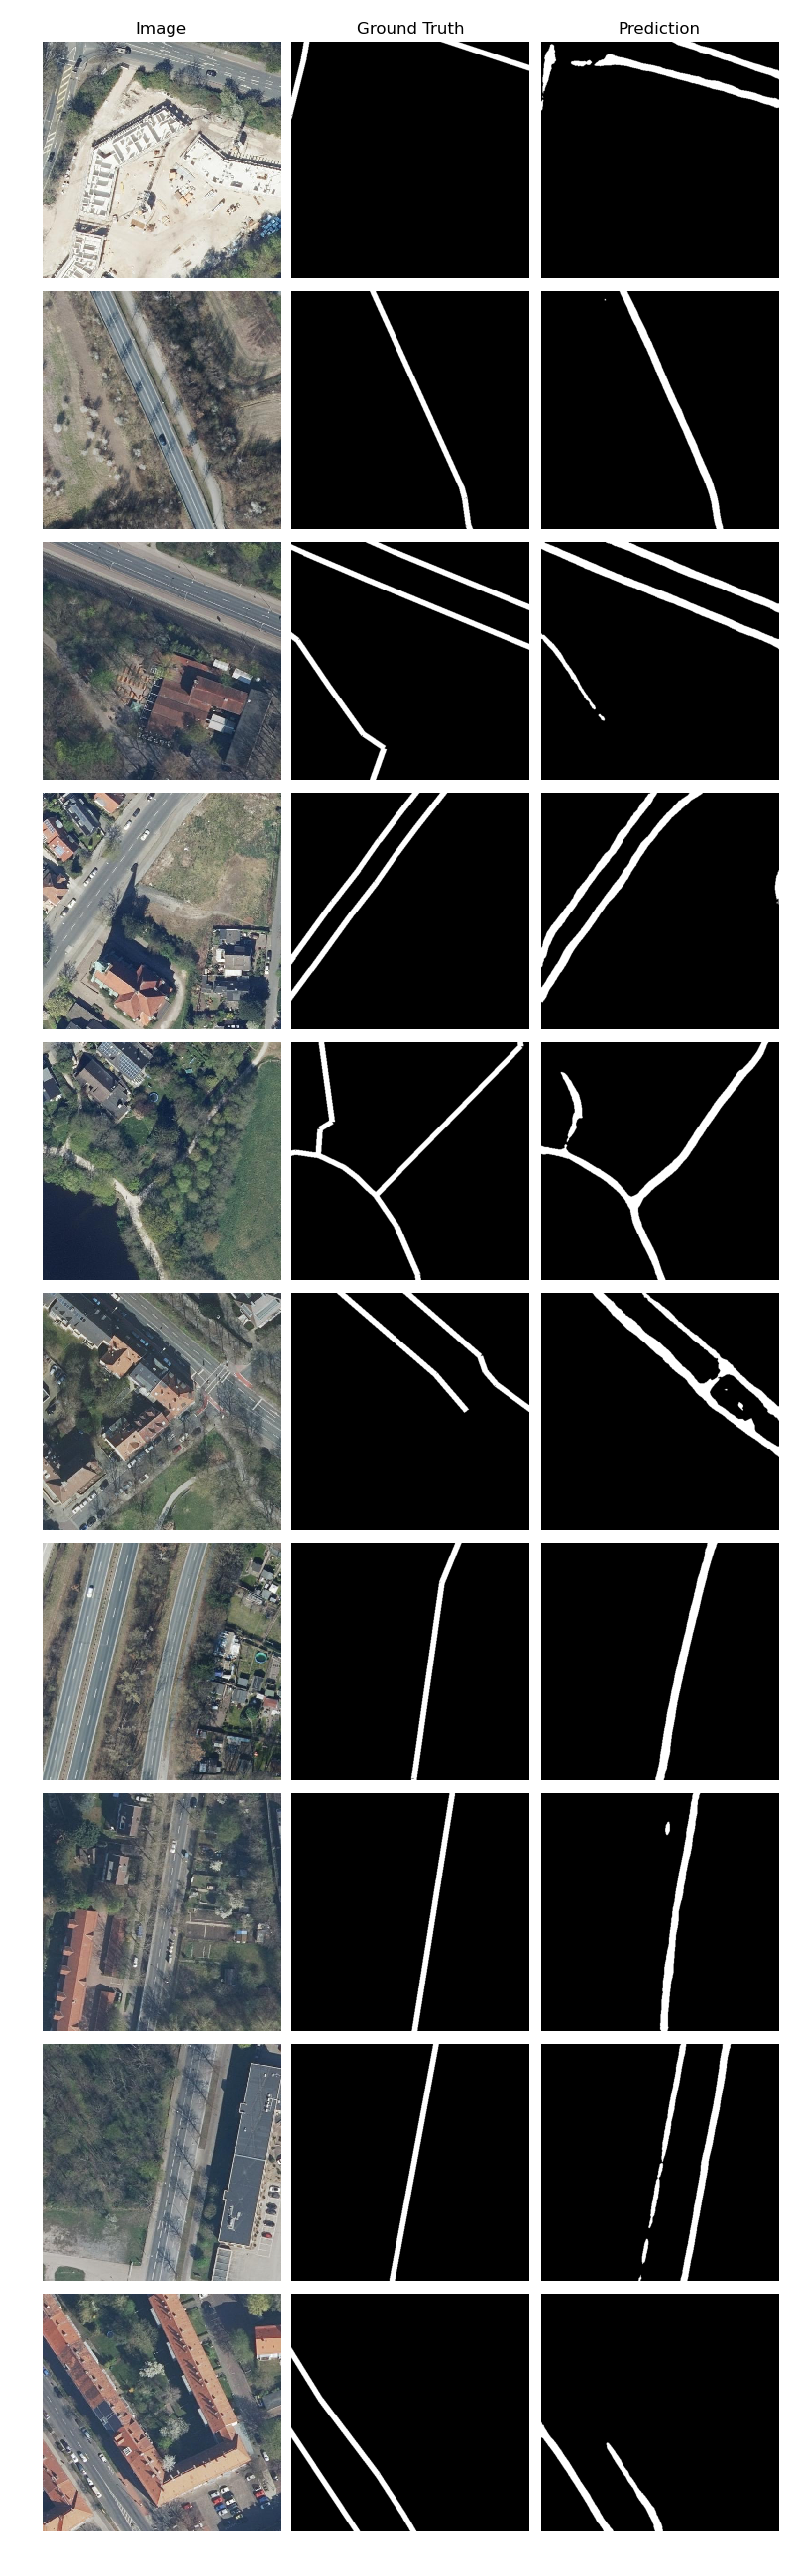
\includegraphics[width=.41\textwidth]{Bilder/Samples-BikeSat/dbunet-r.png} 
	\caption{Beispiel-Predictions des $DBUNet^r$ auf dem BikeSat-Datensatz.}
	\label{fig:bikesat-samples-dbunet-r}
\end{figure}

\begin{figure}
	\centering
	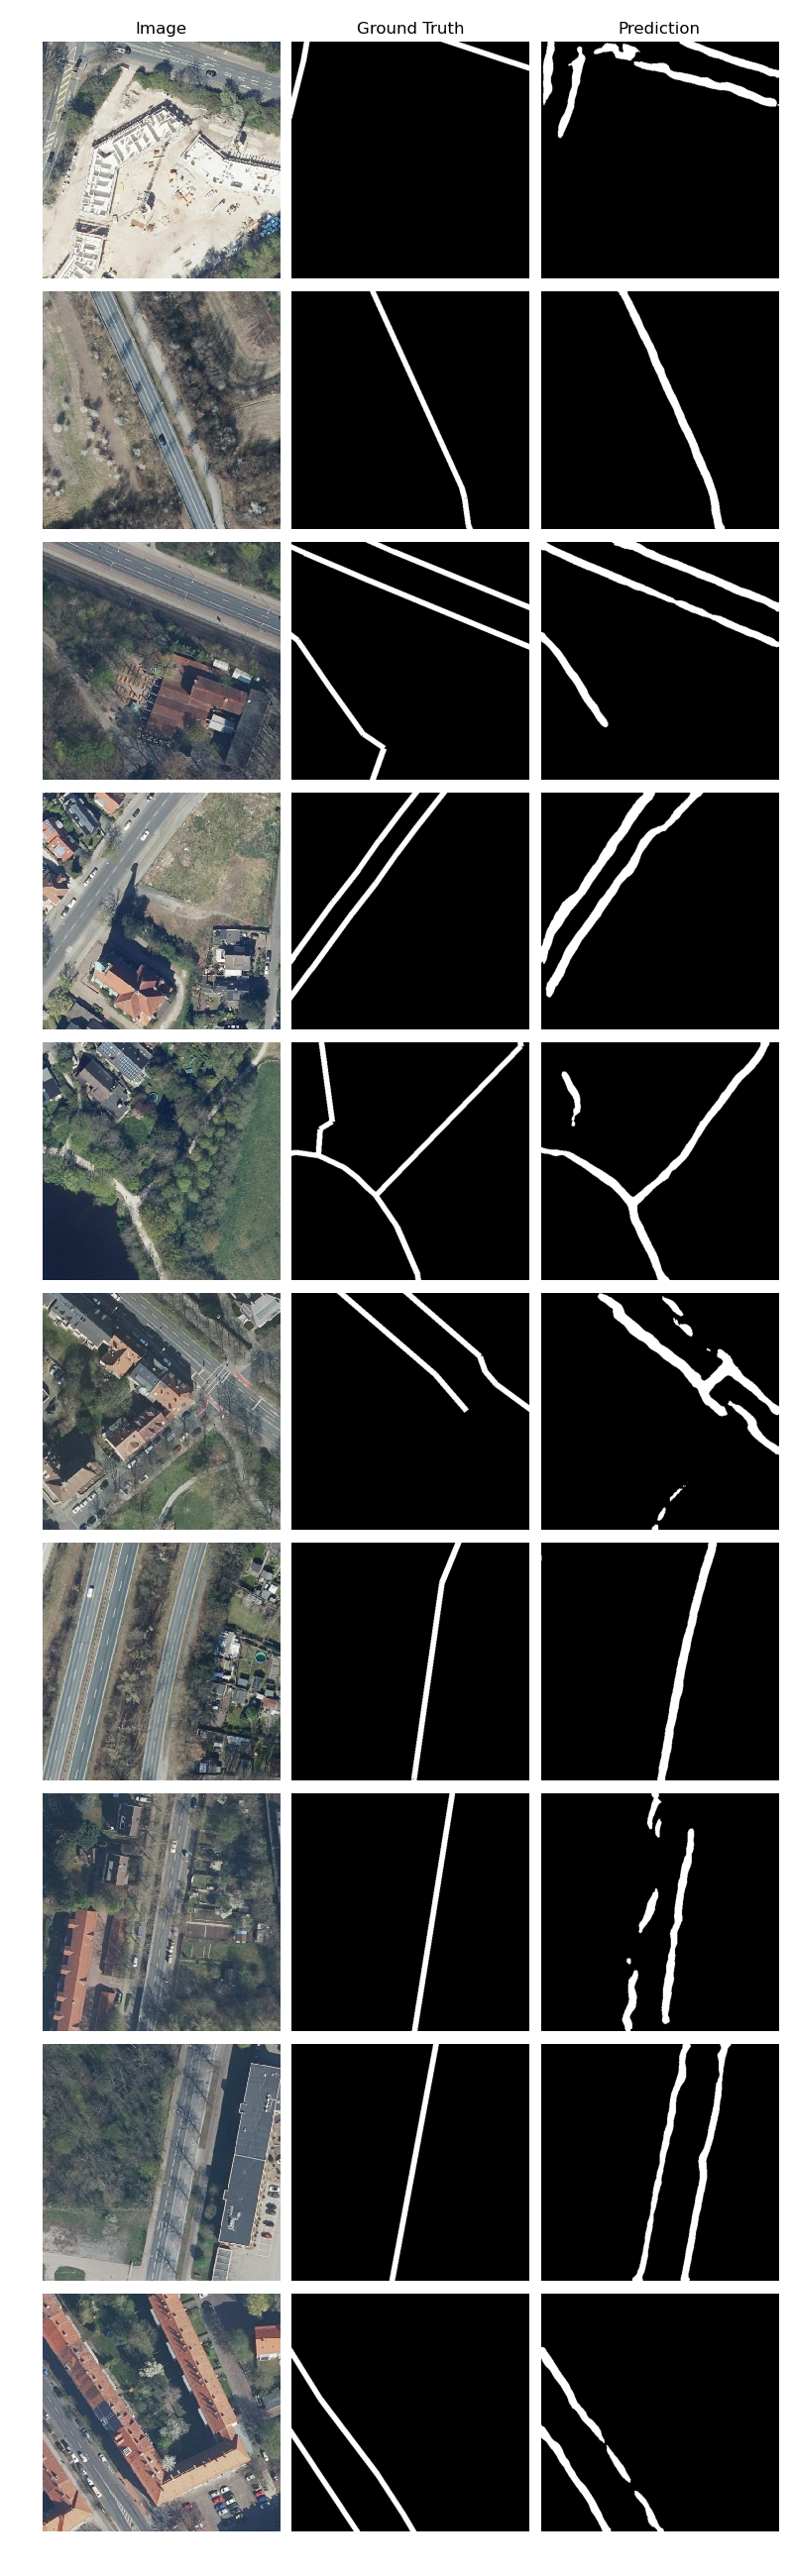
\includegraphics[width=.41\textwidth]{Bilder/Samples-BikeSat/dbunet-s.png} 
	\caption{Beispiel-Predictions des $DBUNet^*$ auf dem BikeSat-Datensatz.}
	\label{fig:bikesat-samples-dbunet-s}
\end{figure}

\begin{figure}
	\centering
	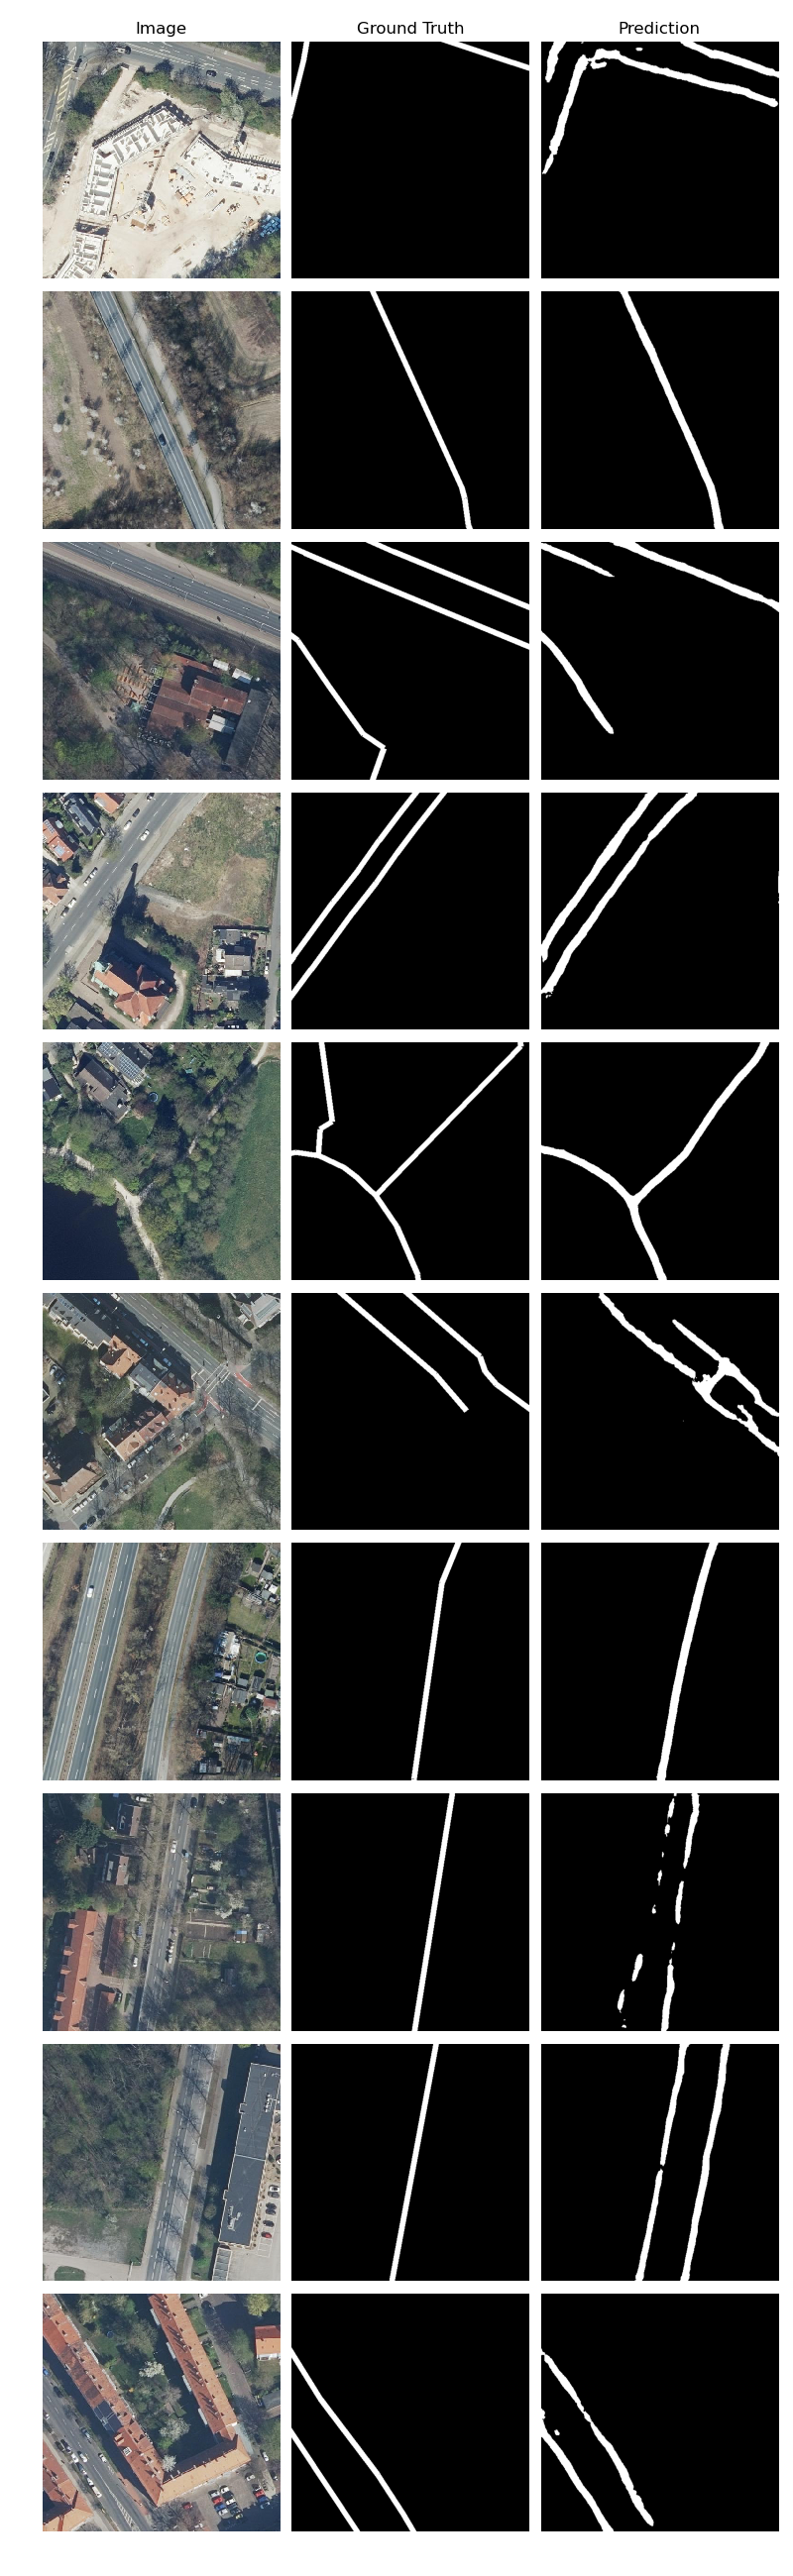
\includegraphics[width=.41\textwidth]{Bilder/Samples-BikeSat/rbunet-l.png} 
	\caption{Beispiel-Predictions des $RBUNet^l$ auf dem BikeSat-Datensatz.}
	\label{fig:bikesat-samples-rbunet-l}
\end{figure}

\begin{figure}
	\centering
	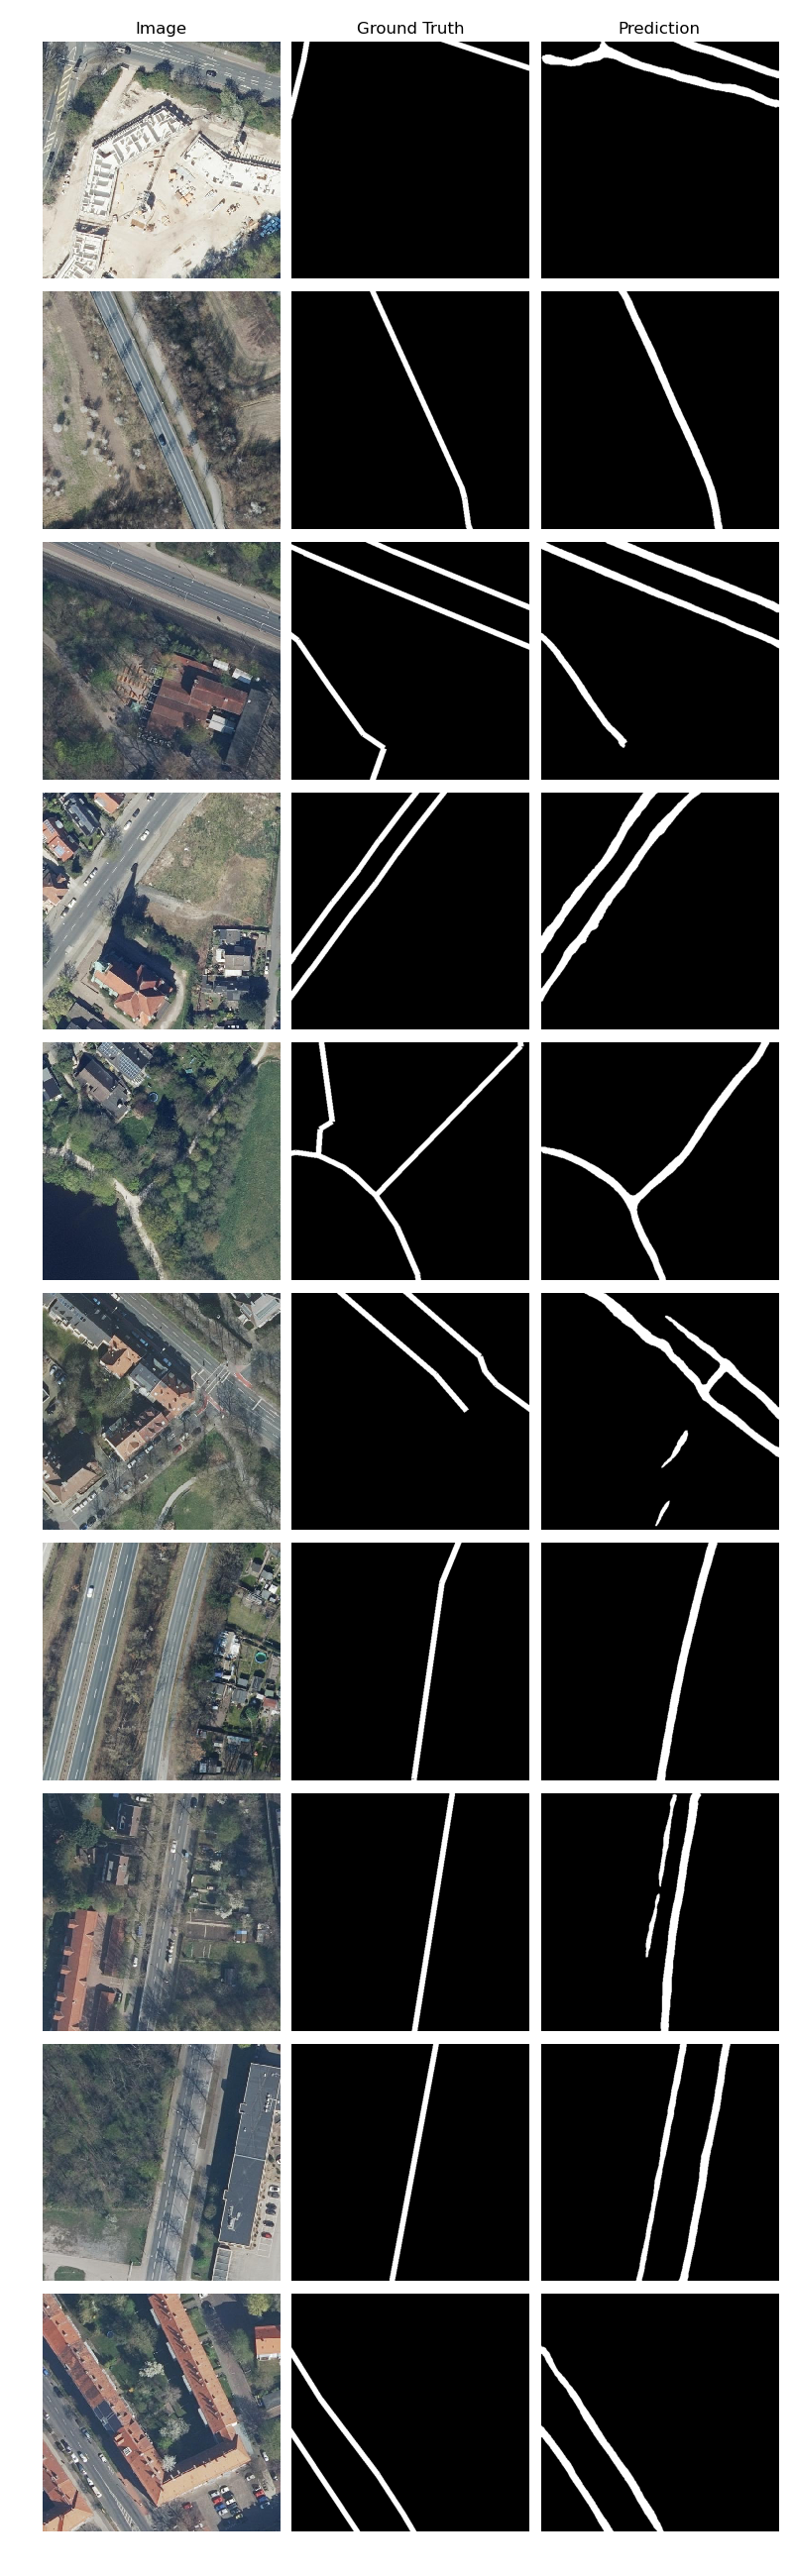
\includegraphics[width=.41\textwidth]{Bilder/Samples-BikeSat/rbunet-r.png} 
	\caption{Beispiel-Predictions des $RBUNet^r$ auf dem BikeSat-Datensatz.}
	\label{fig:bikesat-samples-rbunet-r}
\end{figure}

\begin{figure}
	\centering
	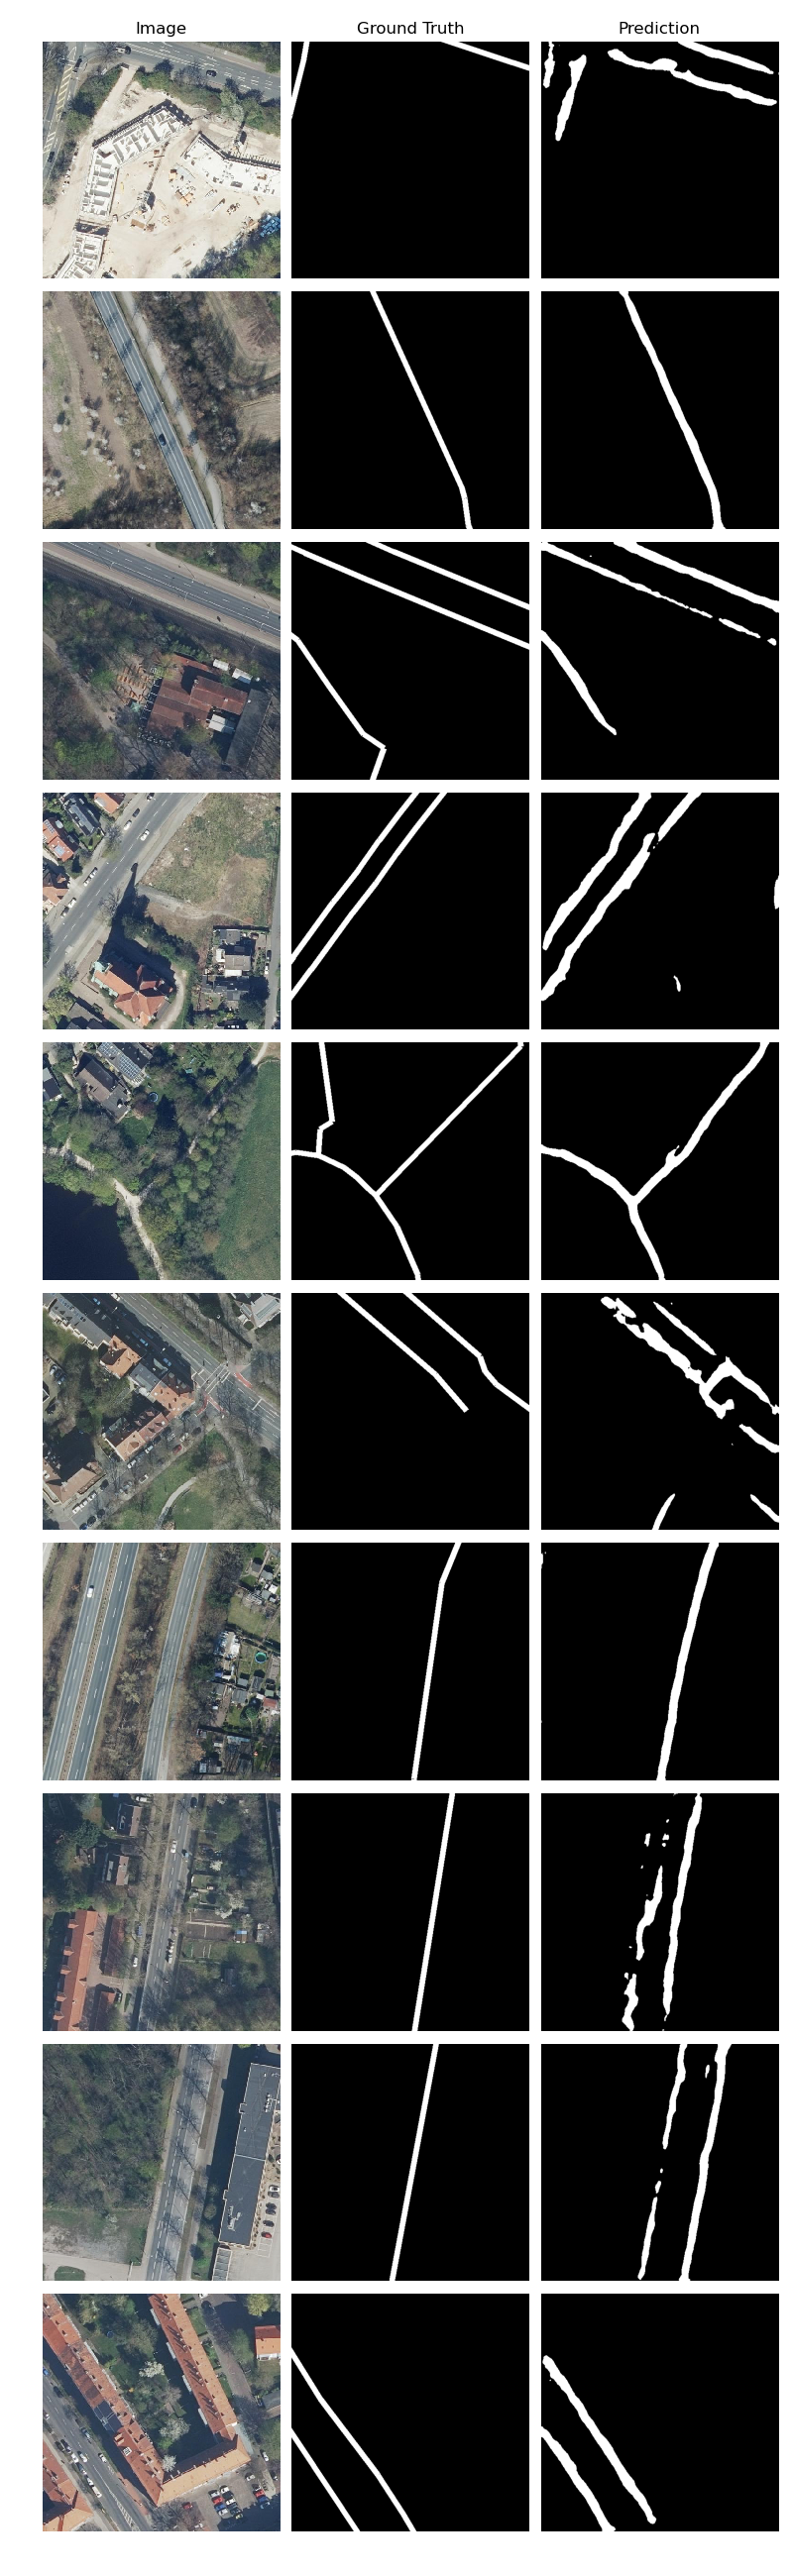
\includegraphics[width=.41\textwidth]{Bilder/Samples-BikeSat/rbunet-s.png} 
	\caption{Beispiel-Predictions des $RBUNet^*$ auf dem BikeSat-Datensatz.}
	\label{fig:bikesat-samples-rbunet-s}
\end{figure}

\begin{figure}
	\centering
	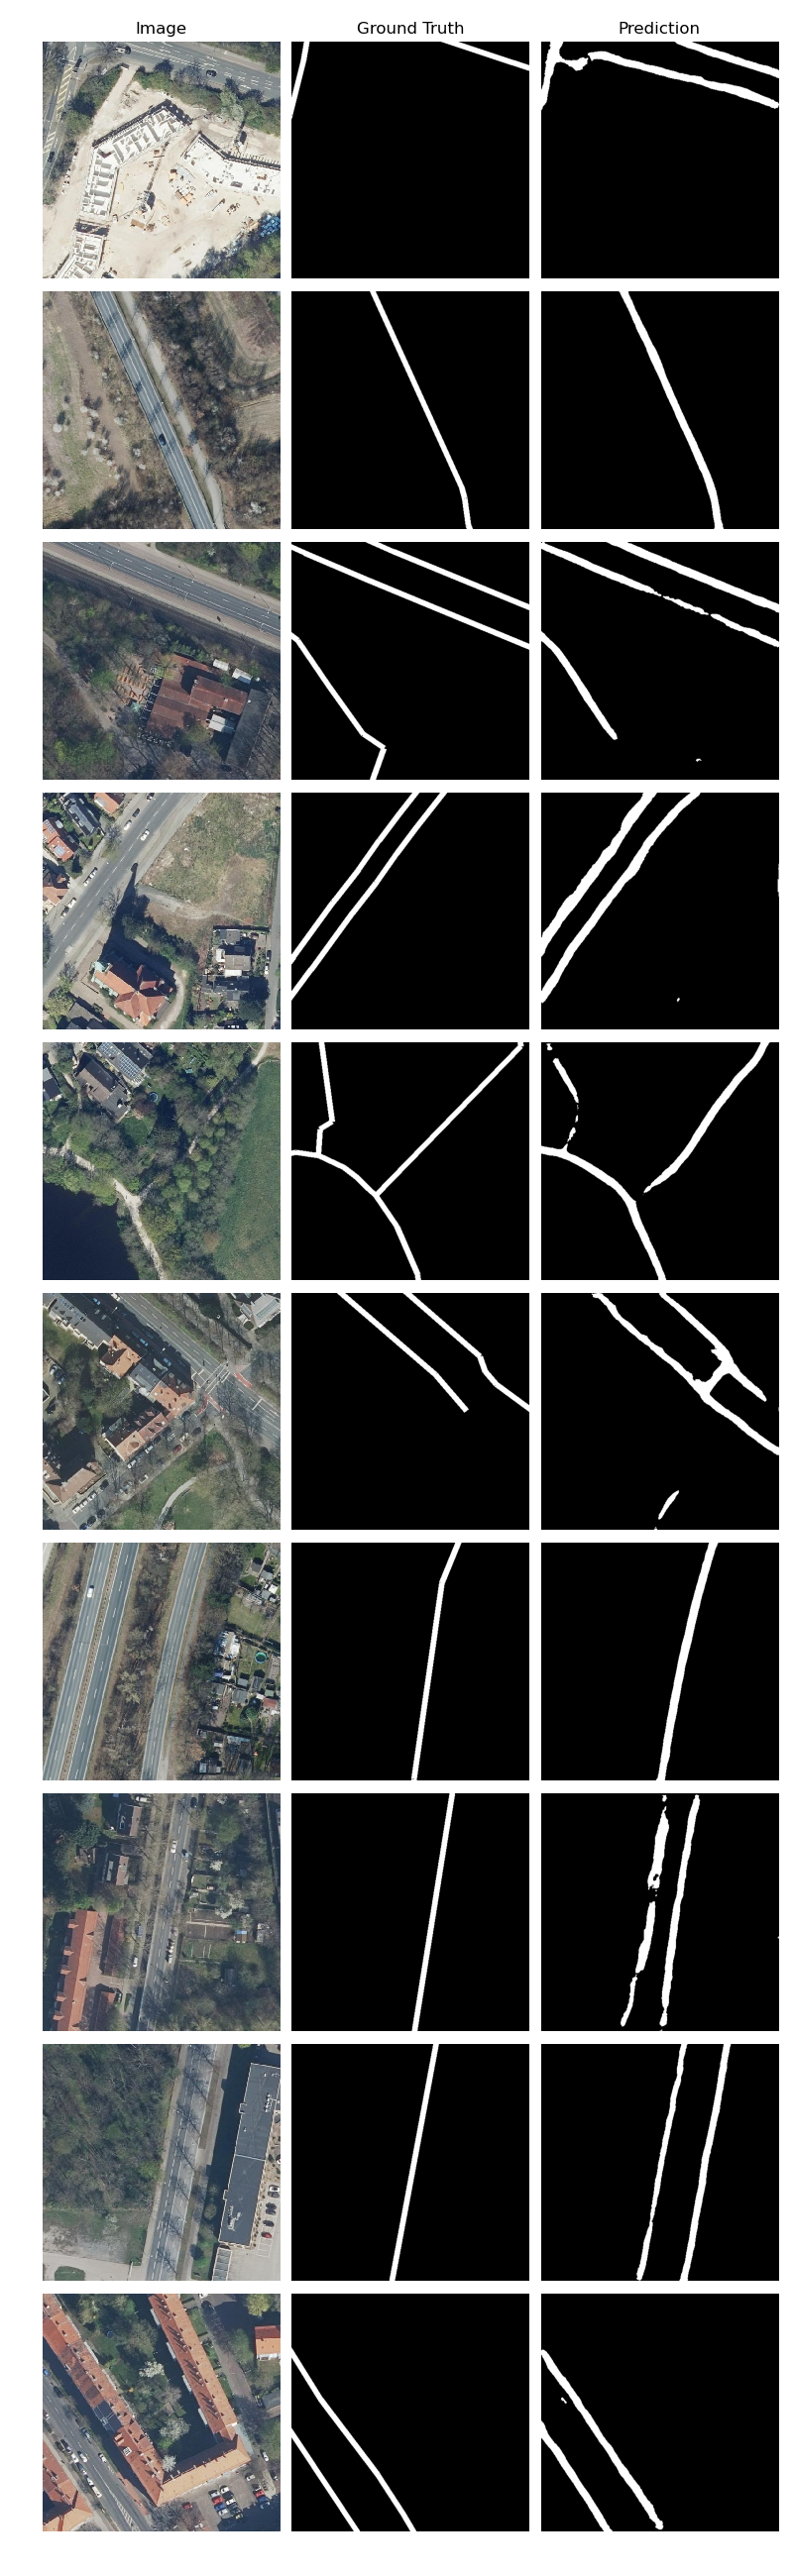
\includegraphics[width=.41\textwidth]{Bilder/Samples-BikeSat/vbunet-l.png} 
	\caption{Beispiel-Predictions des $VBUNet^l$ auf dem BikeSat-Datensatz.}
	\label{fig:bikesat-samples-vbunet-l}
\end{figure}

\begin{figure}
	\centering
	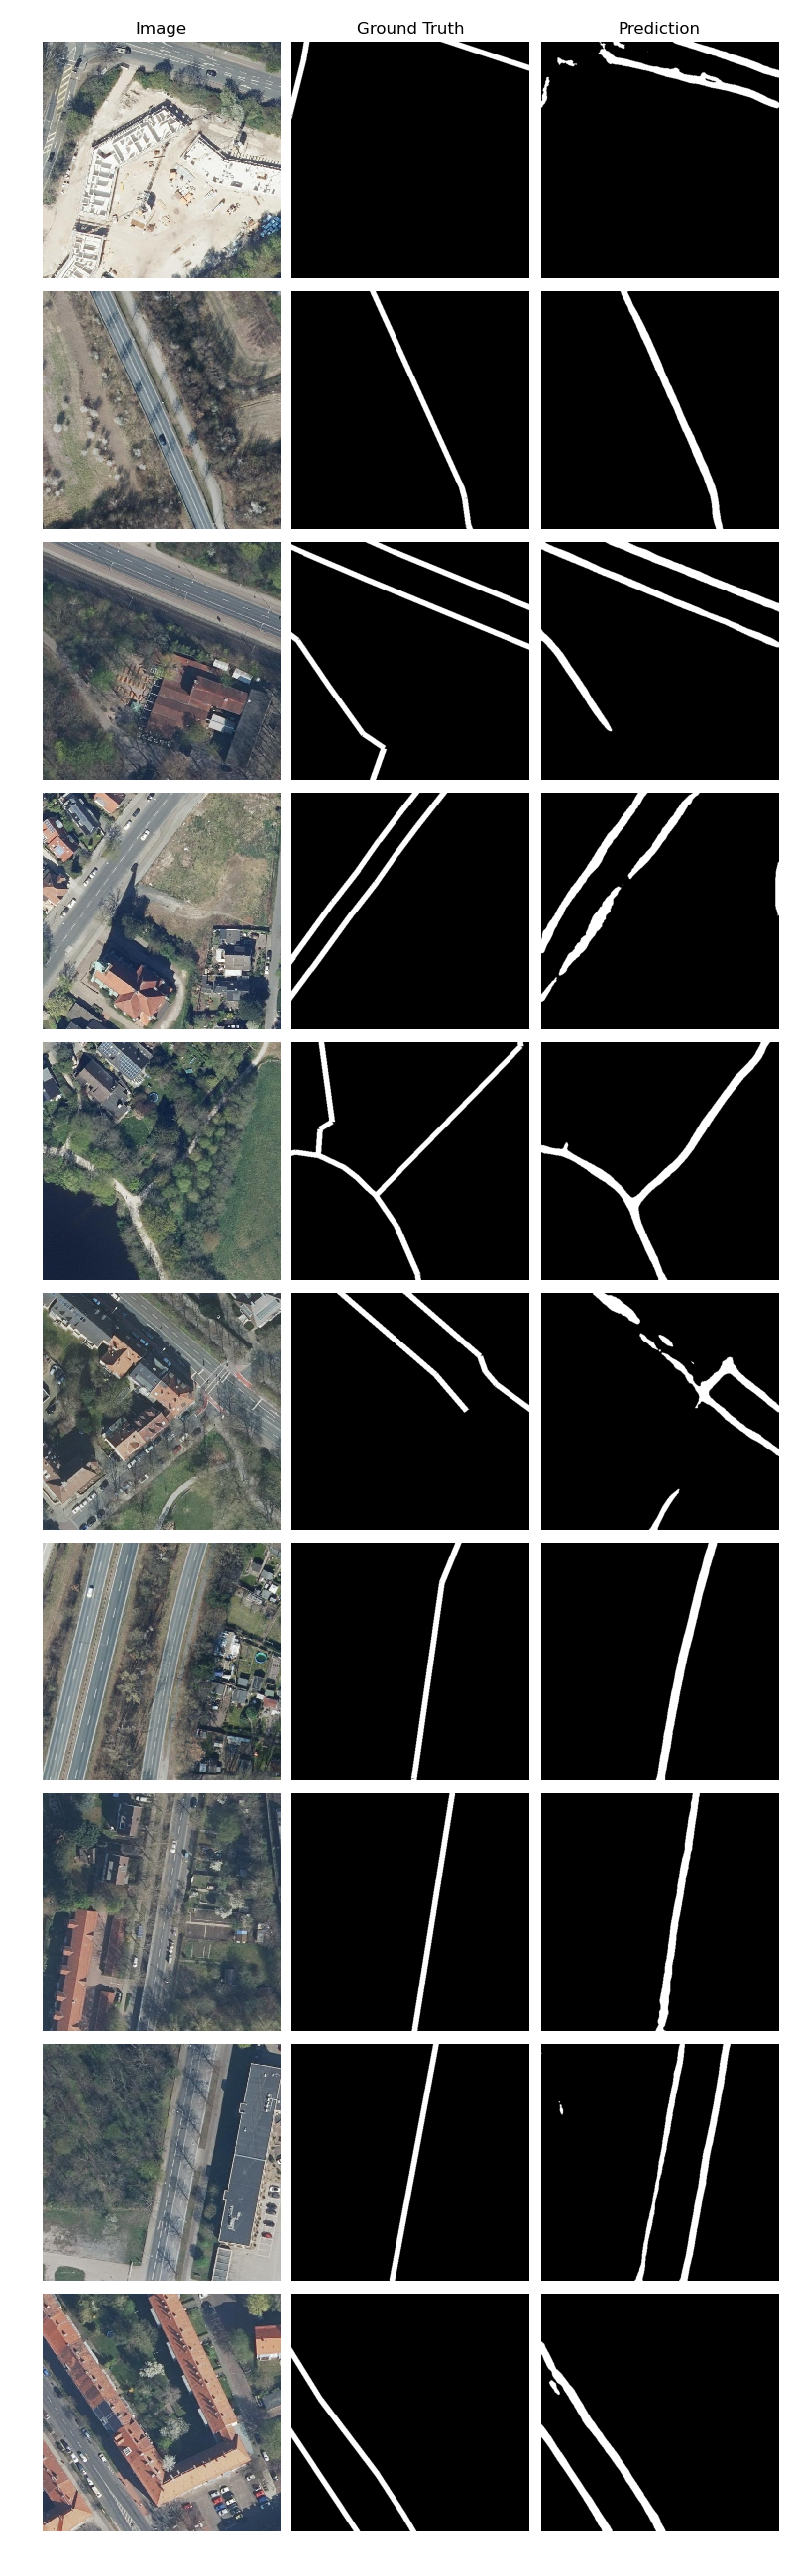
\includegraphics[width=.41\textwidth]{Bilder/Samples-BikeSat/vbunet-r.png} 
	\caption{Beispiel-Predictions des $VBUNet^r$ auf dem BikeSat-Datensatz.}
	\label{fig:bikesat-samples-vbunet-r}
\end{figure}

\begin{figure}
	\centering
	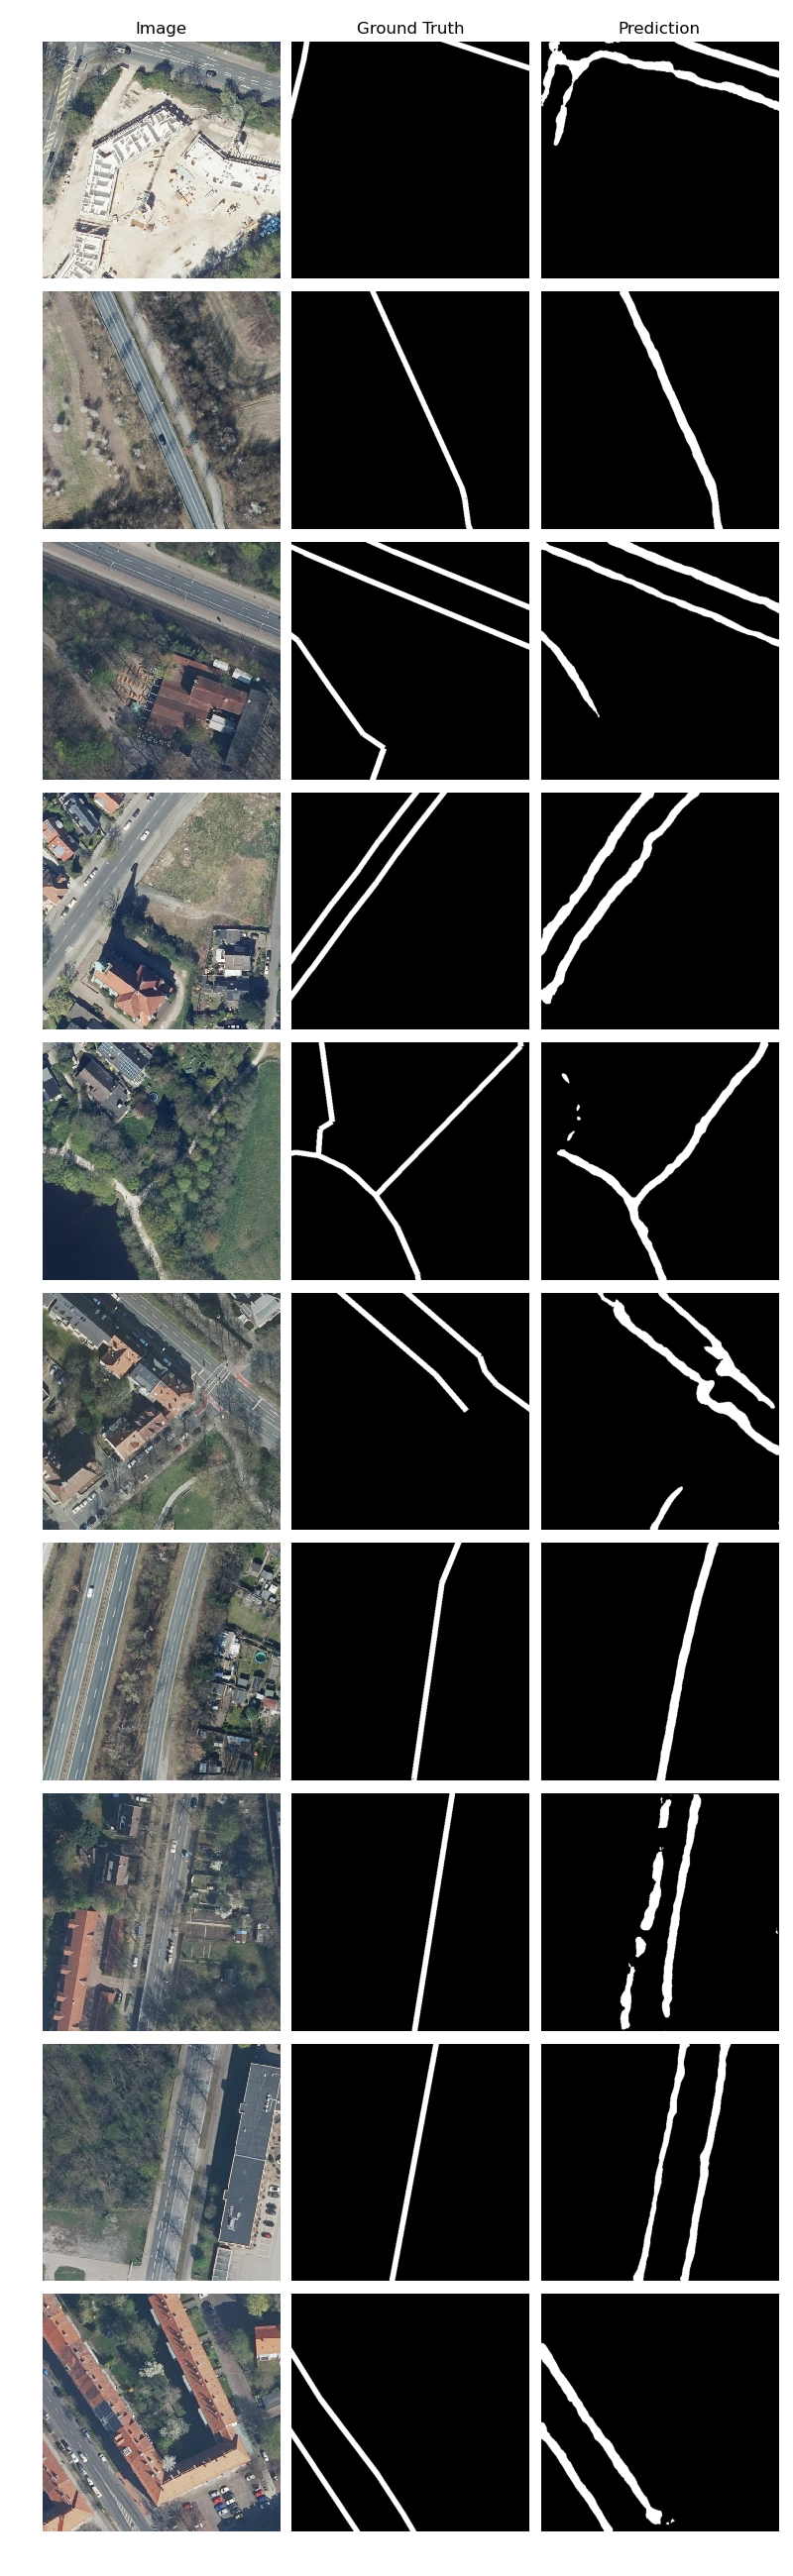
\includegraphics[width=.41\textwidth]{Bilder/Samples-BikeSat/vbunet-s.png} 
	\caption{Beispiel-Predictions des $VBUNet^*$ auf dem BikeSat-Datensatz.}
	\label{fig:bikesat-samples-vbunet-s}
\end{figure}

\pagebreak 


\section{Beispiel-Predictions Karlsruhe}

\begin{figure}
	\centering
	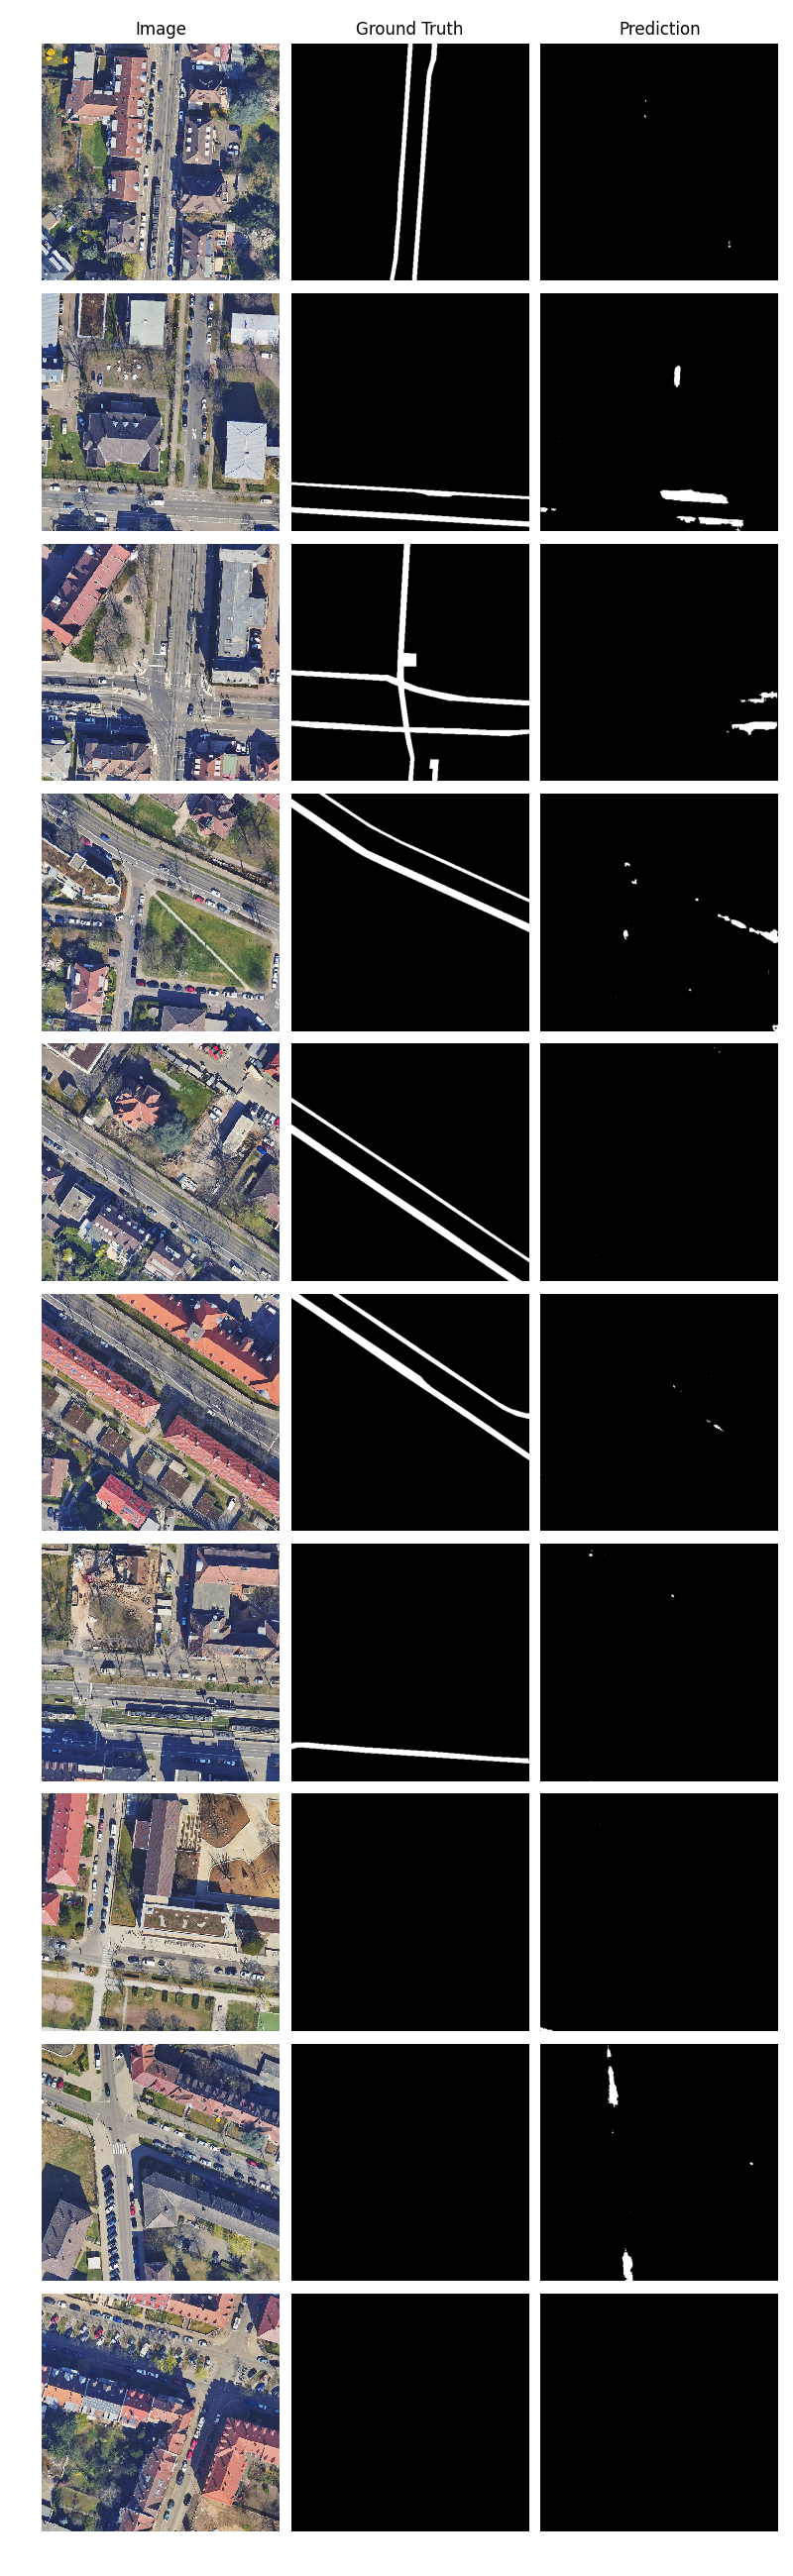
\includegraphics[width=.41\textwidth]{Bilder/Samples-KA/bunet2-l.png} 
	\caption{Beispiel-Predictions des $BUNet2^l$ auf dem Karlsruhe-Datensatz.}
	\label{fig:ka-samples-bunet2-l}
\end{figure}

\begin{figure}
	\centering
	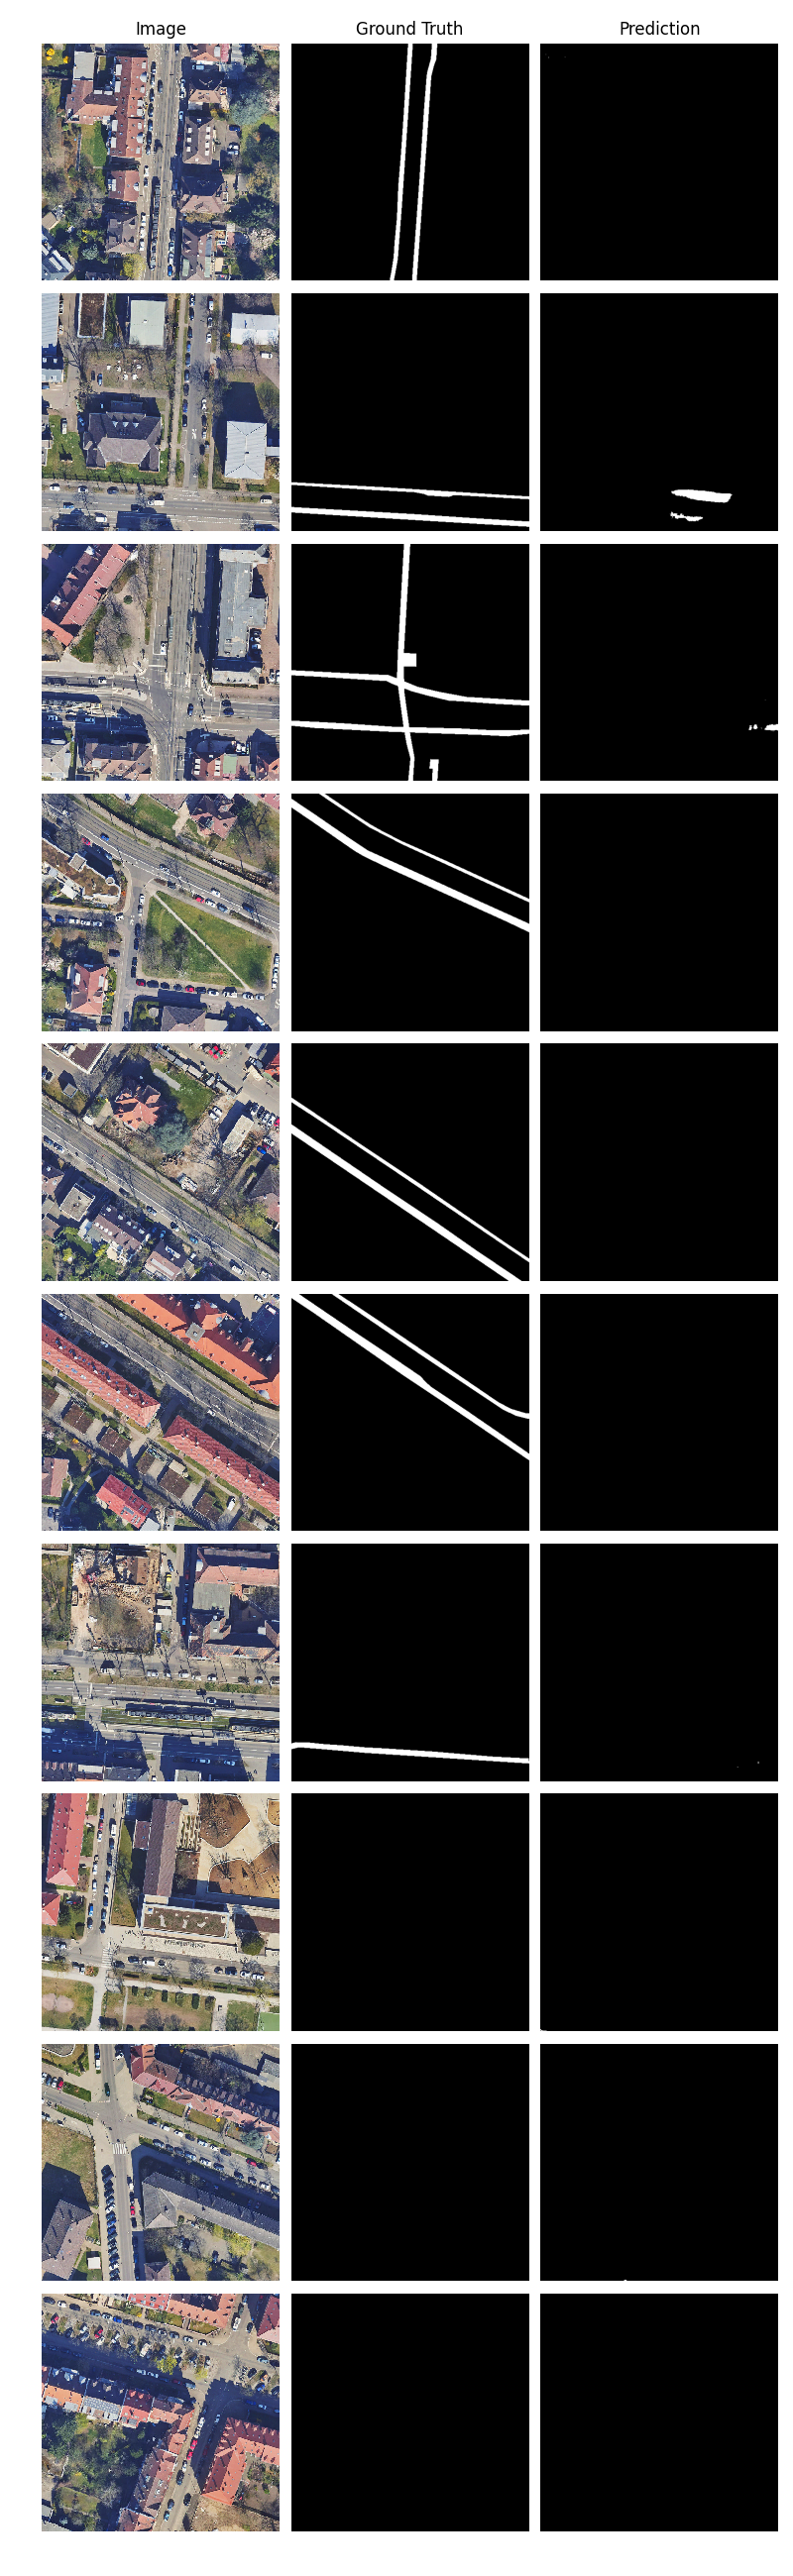
\includegraphics[width=.41\textwidth]{Bilder/Samples-KA/bunet2-r.png} 
	\caption{Beispiel-Predictions des $BUNet2^r$ auf dem Karlsruhe-Datensatz.}
	\label{fig:ka-samples-bunet2-r}
\end{figure}

\begin{figure}
	\centering
	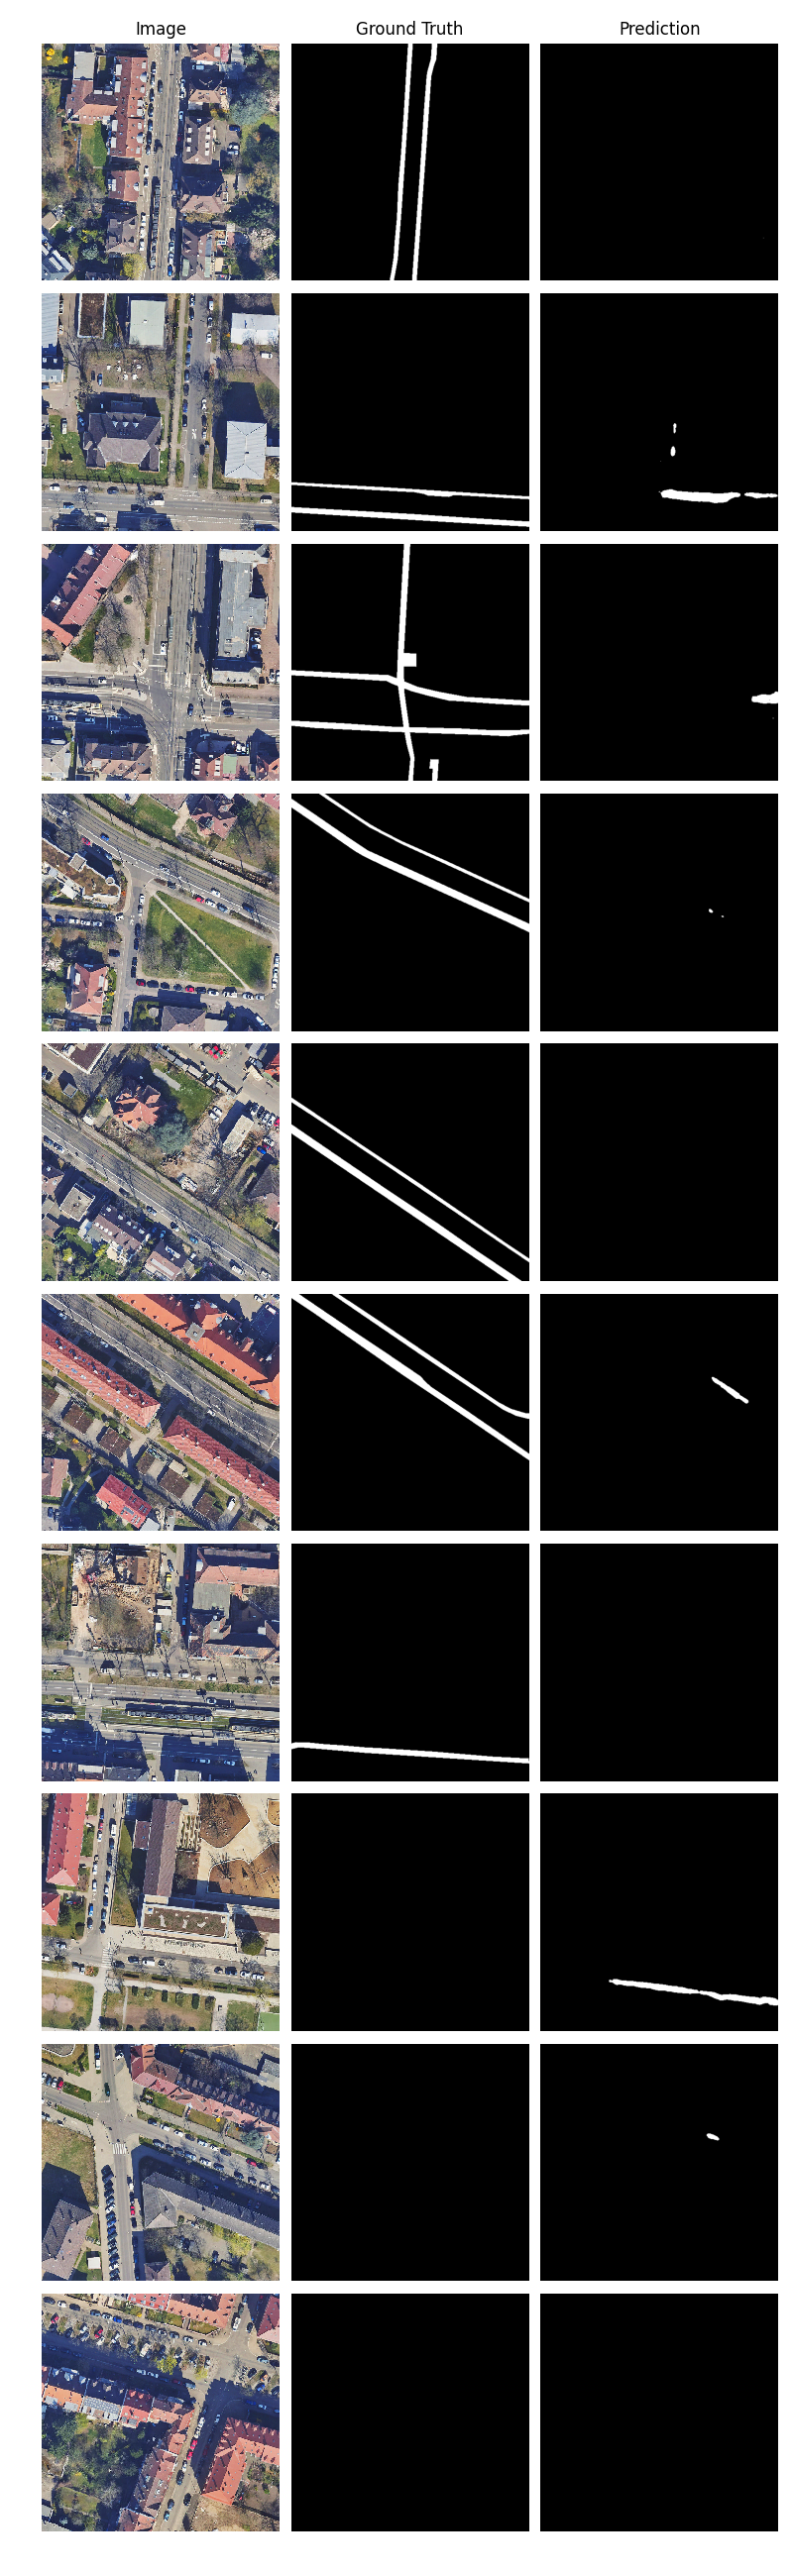
\includegraphics[width=.41\textwidth]{Bilder/Samples-KA/bunet2-s.png} 
	\caption{Beispiel-Predictions des $BUNet2^*$ auf dem Karlsruhe-Datensatz.}
	\label{fig:ka-samples-bunet2-s}
\end{figure}

\begin{figure}
	\centering
	\includegraphics[width=.41\textwidth]{Bilder/Samples-KA/bunet15-l.png} 
	\caption{Beispiel-Predictions des $BUNet15^l$ auf dem Karlsruhe-Datensatz.}
	\label{fig:ka-samples-bunet15-l}
\end{figure}

\begin{figure}
	\centering
	\includegraphics[width=.41\textwidth]{Bilder/Samples-KA/bunet15-r.png} 
	\caption{Beispiel-Predictions des $BUNet15^r$ auf dem Karlsruhe-Datensatz.}
	\label{fig:ka-samples-bunet15-r}
\end{figure}

\begin{figure}
	\centering
	\includegraphics[width=.41\textwidth]{Bilder/Samples-KA/bunet15-s.png} 
	\caption{Beispiel-Predictions des $BUNet15^*$ auf dem Karlsruhe-Datensatz.}
	\label{fig:ka-samples-bunet15-s}
\end{figure}

\begin{figure}
	\centering
	\includegraphics[width=.41\textwidth]{Bilder/Samples-KA/dbunet-l.png} 
	\caption{Beispiel-Predictions des $DBUNet^l$ auf dem Karlsruhe-Datensatz.}
	\label{fig:ka-samples-dbunet-l}
\end{figure}

\begin{figure}
	\centering
	\includegraphics[width=.41\textwidth]{Bilder/Samples-KA/dbunet-r.png} 
	\caption{Beispiel-Predictions des $DBUNet^r$ auf dem Karlsruhe-Datensatz.}
	\label{fig:ka-samples-dbunet-r}
\end{figure}

\begin{figure}
	\centering
	\includegraphics[width=.41\textwidth]{Bilder/Samples-KA/dbunet-s.png} 
	\caption{Beispiel-Predictions des $DBUNet^*$ auf dem Karlsruhe-Datensatz.}
	\label{fig:ka-samples-dbunet-s}
\end{figure}

\begin{figure}
	\centering
	\includegraphics[width=.41\textwidth]{Bilder/Samples-KA/rbunet-l.png} 
	\caption{Beispiel-Predictions des $RBUNet^l$ auf dem Karlsruhe-Datensatz.}
	\label{fig:ka-samples-rbunet-l}
\end{figure}

\begin{figure}
	\centering
	\includegraphics[width=.41\textwidth]{Bilder/Samples-KA/rbunet-r.png} 
	\caption{Beispiel-Predictions des $RBUNet^r$ auf dem Karlsruhe-Datensatz.}
	\label{fig:ka-samples-rbunet-r}
\end{figure}

\begin{figure}
	\centering
	\includegraphics[width=.41\textwidth]{Bilder/Samples-KA/rbunet-s.png} 
	\caption{Beispiel-Predictions des $RBUNet^*$ auf dem Karlsruhe-Datensatz.}
	\label{fig:ka-samples-rbunet-s}
\end{figure}

\begin{figure}
	\centering
	\includegraphics[width=.41\textwidth]{Bilder/Samples-KA/vbunet-l.png} 
	\caption{Beispiel-Predictions des $VBUNet^l$ auf dem Karlsruhe-Datensatz.}
	\label{fig:ka-samples-vbunet-l}
\end{figure}

\begin{figure}
	\centering
	\includegraphics[width=.41\textwidth]{Bilder/Samples-KA/vbunet-r.png} 
	\caption{Beispiel-Predictions des $VBUNet^r$ auf dem Karlsruhe-Datensatz.}
	\label{fig:ka-samples-vbunet-r}
\end{figure}

\begin{figure}
	\centering
	\includegraphics[width=.41\textwidth]{Bilder/Samples-KA/vbunet-s.png} 
	\caption{Beispiel-Predictions des $VBUNet^*$ auf dem Karlsruhe-Datensatz.}
	\label{fig:ka-samples-vbunet-s}
\end{figure}
%\clearpage
%\pagenumbering{Roman}  % römische Seitenzahlen für Anhang

\newpage
\end{document}
